\documentclass[uplatex,dvipdfmx]{jlreq}

\usepackage{jlreq-deluxe}
\usepackage[noalphabet,hiragino-highsierra-pron]{pxchfon}
\usepackage[T1,LGR]{fontenc}
\usepackage{stix2}
\usepackage{roboto}
\usepackage[scale=0.95]{roboto-mono}

\usepackage[fleqn,tbtags]{mathtools} % 数式関連 (w/ amsmath)
\usepackage[table,dvipdfmx]{xcolor}
\usepackage[dvipdfmx]{graphicx}
\usepackage{ascmac} %screen/itembox/shadebox環境が使用できる．
\usepackage{float} % 表・図の[H]配置指定に必要
\usepackage{placeins} % \FloatBarrierで図表が節をまたがないようにする
\usepackage{longtable} % 1ページに収まらない表をページをまたいで表示するために必要
\usepackage{siunitx} % \SI{}{}による単位表記に必要
\usepackage{pgfgantt}
\usepackage{tikz}
\usetikzlibrary{arrows.meta,fit,positioning}

\usepackage[dvipdfmx]{hyperref}
\hypersetup{%
 bookmarksnumbered=true,%
 colorlinks=true,%
 linkcolor=black,
 citecolor=blue,
 urlcolor=blue}
\usepackage[dvipdfmx]{pxjahyper} % (u)pLaTeXのときは必要
\usepackage{listings,plistings}
\renewcommand{\lstlistingname}{コード} % キャプションの接頭辞を「Listing」から「コード」に変更
\lstset{%
	aboveskip=0pt,
	belowskip=0pt,
	language=C++, % Arduinoのスケッチの関数も多くカバーできる．
	morekeywords={ },
	numbers=left,          % 行番号を左に表示
	numberstyle=\small,    % 行番号のフォントサイズ
	stepnumber=1,          % 行番号を何行おきに表示するか
	numbersep=10pt,        % 行番号とコードの間の距離
	backgroundcolor={},% 
	basicstyle={\small\ttfamily},% 
	keywordstyle=\color{blue}\bfseries,
	commentstyle=\color{red},
	frame=single,
	breaklines=true}

\newcommand{\mcbf}[1]{{\mcfamily\bfseries #1}}
\newcommand{\gtbf}[1]{{\sffamily\bfseries #1}}
\renewcommand\UrlFont{\color{blue}\rmfamily}

\usepackage{hira-stix} % ヒラギノフォント＆STIX2 代替フォント定義（Warning回避）

\begin{document}

\begin{titlepage}
\vspace*{1cm}
\centering
\Huge\textsf{回転機構のレーザー受光と楽器間無線通信による同期・輪唱システム}\\[2cm]
\Large\textsf{情報工学科 2年}\\
\Large\textsf{24G1059}\\[5pt]
\huge\textsf{佐藤　涼菜}

\vspace*{1cm}
\Large\sffamily
\begin{itembox}[c]{チーム40}
\centering
\begin{tabular}{ll}
宇井 祐真（24G1021）&
梅野 大誠（24G1026）\\
山口 侑希（24G1136）&
薄井 悠希（25G1020）\\
菊池 侑人（25G1041）&\\
\end{tabular}
\end{itembox}

\vspace*{1cm}
\Large\textsf{\today}
\end{titlepage}
\clearpage

%% 以降本文
\section{はじめに}
\label{sec:hajimeni}
\subsection{社会的背景・課題・本稿の目的}

近年，動画配信サイトやストリーミングサービスの普及によって，誰もが手軽に音楽コンテンツを視聴できる環境が整っている．特に日本では，ゲームやアニメなどのサブカルチャーを起点とした音楽コンテンツが数多く生み出されており，独自の文化として定着している．
一方で，このようなデジタル配信の消費形態は，実際に会場へ足を運んで演奏を体感するライブイベントやコンサートとの相乗効果を生み，市場規模の拡大にも寄与している\cite{cul}\cite{live}．たとえば，博報堂の谷口による分析では，ストリーミングサービスの利用者がサービス内で新たに好みのアーティストを複数発掘し，そのアーティストたちを一度に鑑賞できるライブやフェスへ参加するという行動の流れが形成されつつあり，さらにライブでの体験を通じて別のアーティストと出会うことで，再びストリーミングでの視聴に戻るという音楽消費サイクルが生まれていると指摘されている\cite{taniguchi2019}．すなわち，デジタル配信とライブイベントは互いの顧客を送客し合う関係にあり，この循環が音楽市場全体の拡大を後押ししていると考えられる．実際に，一般社団法人コンサートプロモーターズ協会が実施したライブ市場調査によれば，2025年におけるライブ市場の年間売上高は6443億円，入場者数は5999万人にのぼり，デジタル配信の普及以降もライブ市場は堅調に拡大を続けている\cite{acpc}．図\ref{fig:live_market}に示すように，国内のライブ・コンサート市場における年間売上額は2010年の1280億円から2019年の3665億円まで，10年間でおよそ2.9倍に拡大している．2020年には新型コロナウイルス感染症の影響により，会場に人を集めること自体が困難となった結果，年間売上額は779億円まで急落した．しかし，行動制限の緩和とともに市場は急速に回復し，2022年には3984億円，2023年には5140億円，そして2025年には過去最高となる6443億円を記録している．この推移から，ライブ会場に足を運ぶという体験に対する需要は，一時的な外的要因によって落ち込むことはあっても，長期的には一貫して拡大する傾向にあると言える．

\begin{figure}[tb]
  \centering
  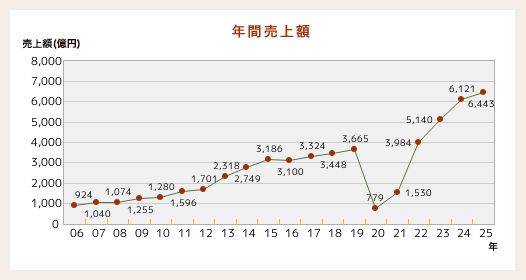
\includegraphics[width=0.7\linewidth]{figs/acpc_sales_transition.png}
  \caption{国内ライブ・コンサート市場における年間売上額の推移（一般社団法人コンサートプロモーターズ協会「基礎調査推移表」より)}
  \label{fig:live_market}
\end{figure}

デジタル配信が普及していく中で，なぜデジタル配信では代替できない価値がライブ会場に存在するのだろうか．その理由の一つとして，ライブ演出に用いられる音響や照明，ライブ参加者自身が感じる振動といった複数の物理的刺激が挙げられる．これらの刺激は，観客一人ひとりに個別に届けられるのではなく，同じ空間にいる観客全員に同時に共有されるという性質を持つ．その結果，観客同士が同じ体験を共有しているという感覚，すなわち空間全体としての一体感が形成される．換言すれば，ライブ会場における没入感とは，ユーザが音楽を聴くだけでとどまらない，物理的，視覚的な技術を同じ空間で同時に受け取ることによって生まれる体験だと考えられる．
この仮説は，複数の研究によっても裏付けられている．ライブ演奏とデジタル配信を直接比較した実証研究によっても裏付けられている．
Kreuzerら（2025）は，同一のクラシック音楽コンサートを，会場で聴取する条件と映像配信で視聴する条件とで比較する実験を行った．その結果，没入感や社会的なつながりの感覚を含む複数の評価軸において，ライブ条件の方が配信条件よりも有意に高い評価を得ることを示した\cite{Kreuzer2025}．すなわち，同じ演奏内容・同じ音質であっても，同じ空間を他の観客と共有しているという感覚そのものが，没入感を左右する独立した要因であり，これは録画・配信技術の高度化だけでは補えないことを意味する．したがって，音そのものの再現性だけでなく，ライブ体験に固有の空間的フィードバックを組み込むことで没入感の高い演奏体験の実現に有効であると考える．

また，Natalia Cooperら（2018）は，仮想現実（VR）環境における体験の再現度を高めるため，視覚情報のみでは表現が難しい感覚を，音や触覚など別の感覚を用いた代替フィードバックとして提示する実験を行った．その結果，視覚刺激のみを提示した場合と比較して，音や触覚といった複数の異なる刺激を組み合わせて提示した場合の方が，利用者の没入感・関与感が有意に高まることを明らかにした\cite{Natalia2018}．つまり，複数の感覚情報を同時に提示する多感覚的フィードバックは，ユーザの体験における没入感の向上に有効であると考える．また，Human-Computer Interaction（HCI）分野の知見も同様の傾向を支持している．Martinら（2024）は，ライブコンサート環境を対象とした研究において，観客が演奏を受動的に聴取するだけでなく，能動的に体験へ参加することが，会場全体の活気や観客の感情の高まりに寄与すると結論づけた\cite{Martin}．よって，ユーザ自身が能動的に関与できる仕組みもまた，システムの没入感を高める要因として重要であると考える．

一方，音楽を自動で演奏する自動演奏技術の分野では，デジタル技術の発展により高精度な同期や楽曲再現が可能になっている．たとえば，Yamahaが提供するDisklavier ENSPIREシリーズは，光学センサとサーボモータを用いて演奏情報を高精度に再現するとともに，鍵盤が実際に動作する様子をユーザへ視覚的にフィードバックを行う機能を備えている\cite{yamaha}．しかし，この視覚的フィードバックは，ピアノの鍵盤という限られた範囲でのみ提示されるものであり，その場に居合わせたユーザ１人のみが確認できる情報にとどまる．したがって，複数人が同じ空間にいる状況を想定すると，自動演奏技術によって提示される視覚的フィードバックは，空間全体には行き渡らないという限界を抱えていると言える．

以上を踏まえると，現状の自動演奏技術は，演奏そのものの精度は高い一方で，前述した「多感覚的フィードバック」と「空間全体への共有」という，没入感を高めるうえで重要な要素を十分には満たせていないという課題が生じる．特に，Kreuzerらの知見が示すとおり，同じ場を共有しているという空間的なフィードバックは，音質や演奏精度をいくら高めても代替できない，ライブ体験に固有の要素である．したがって，デジタル配信や高精度な自動演奏技術がどれほど発展しても，この空間的フィードバックを欠いたままでは，ライブ会場に匹敵する高い没入感を得ることはできないと結論づけられる．そこで本稿では，自動演奏技術に，ライブ体験に共通するこの空間的フィードバックを付加した楽器間通信システム「回転機構のレーザー受光と楽器間無線通信による同期・輪唱システム」を提案する．本システムは，ユーザの動作を検知する指揮デバイス，指揮デバイスからの情報に応じ回転する観覧車型の中継機デバイス，そして中継機からのレーザー光を受光し演奏を行う楽器デバイスによって構成される．指揮デバイスによるユーザの能動的な動作，観覧車型デバイスによる空間全体への視覚的なフィードバックの共有，そして高精度な音色の演奏による聴覚的な刺激を組み合わせることで，従来の自動演奏技術では実現が難しかった，会場全体を巻き込む没入感の高い演奏体験の提供を目指す．

\subsection{類似技術・先行研究}

本節では，本システムの独自性を明確にするため，音楽に視覚的なフィードバックを付加する既存技術を整理し，それぞれの特徴と限界を検討する．

第一に，DMX512信号（以下，DMX信号と表記する）を用いた照明制御システムが挙げられる．DMX信号とは，舞台照明の操作卓と調光機との間でデータをやり取りするための通信規格であり，現在では舞台演出やコンサートにおいて，音楽に合わせた光量制御を行う目的で広く利用されている\cite{sekine2021}．このシステムは，音楽という聴覚的な刺激に加えて光という視覚的な刺激を提示することで，観客の没入感を高めることができる．しかし，DMX信号による照明制御は，あらかじめプログラムされた演出を再生する仕組みであるため，観客はその光の変化を一方的に受け取る，すなわち受動的に認識する立場にとどまる．前節で述べたとおり，能動的な関与が没入感を高める要因の一つであることを踏まえると，観客が演奏そのものに関与できないDMX信号による演出には限界があると言える．この課題に対し，本提案では指揮デバイスを導入し，利用者が指揮という身体動作を通じて演奏そのものを能動的に制御できるようにすることで，身体的な関与に基づく没入感の向上を狙う．

第二に，物理的な操作によって音楽を制御するタンジブル・インターフェースの例として，ReacTableが挙げられる．ReacTableは，卓型のディスプレイ上に複数の物理モジュールを配置し，その配置や動きに応じて音を合成するシンセサイザの一種であり，利用者は身体的な物理操作を通じて演奏を制御するとともに，ディスプレイに表示される視覚的な情報によって演奏状態のフィードバックを受け取ることができる\cite{reactable}．しかし，この視覚的フィードバックはディスプレイという限られた表示領域内で完結しており，操作を行う利用者本人以外の第三者や，会場全体へフィードバックを共有する仕組みとしては設計されていない．そこで本提案では，指揮デバイスに加えて観覧車型の中継機デバイスを導入する．観覧車型デバイスが演奏情報に応じて回転する様子を，利用者本人だけでなく周囲にいる第三者も視認できるようにすることで，演奏状態の把握や共有を空間全体に広げ，多感覚的なフィードバックを実現することを狙う．

以上のように，DMX信号による照明制御は観客の能動的な関与を欠き，ReacTableのような既存のタンジブル・インターフェースは視覚的フィードバックが個人の操作範囲内にとどまるという，それぞれ異なる限界を抱えている．本提案は，指揮デバイスによる能動的な演奏制御という既存研究の知見と，観覧車型デバイスによる空間共有性という要素を組み合わせることで，これら二つの課題を同時に解決し，空間全体への多感覚的なフィードバックを通じて，利用者の没入感および関与感を高めることを目指す．

\section{作成したシステムの概要}
本節では，作成したシステムの概要について説明する．本システムは，ユーザの能動的な動作と連動した観覧車型中継機デバイスの回転およびレーザの発光を通じて，演奏空間全体に多感覚なフィードバックを与えることで，従来の自動演奏技術における演奏インターフェースでは得られない高い没入感をユーザに提供することを目的として設計されている．
本システムは，指揮デバイス，観覧車型の中継機デバイス，楽器デバイスという３つのデバイスから構成される．
% まず，本システムの全体の構成図を図\ref{zentai}に示す．ユーザが指揮デバイスに取り付けられたボタンを押下すると，同期開始情報が無線通信によって中継機デバイスおよび楽器デバイスへ送信され，中継機デバイスが作動を開始する．
演奏開始後，ユーザがスライド式可変抵抗器を操作したうえで指揮デバイスを振ると，加速度センサが振り動作を検知し，中継機デバイスが

ここからは各デバイスの概要について説明する．

\begin{figure}[h]
    \centering
     \centering
    \includegraphics[width=15cm]{./figs/zentai.png}
    \caption{全体の構成図}
    \label{zentai}
\end{figure}
    
    

\subsection{指揮デバイス}
\subsubsection{概要}
まず，指揮デバイスについて説明する．指揮デバイスのシステム構成図を図\ref{fig:sys_siki}に示す．本デバイスは，演奏全体を統括するデバイスであり，主に以下の３つの機能を有する．
第一の機能は，演奏開始トリガーの送信である．ユーザが指揮デバイスに搭載されたタクトスイッチを押下すると，中継機デバイスと楽器デバイスへ演奏開始トリガーを送信する．さらに，中継機デバイスの回転が開始される．

第二の機能は，楽曲のBPM変更である．ユーザがスライド式可変抵抗器を操作した後，デバイスを振ると新しい設定BPM情報が中継機デバイスへ送信される．これにより，中継機デバイスのモータ回転速度がこの値に追従して変化する．そして，その回転に伴うレーザーの通過光を介して各楽器デバイスに情報が伝達され，BPMの変更される．また，楽曲のBPMは5段階に分けて変更できる．

第三の機能は，楽曲の音量変更である．ユーザがスライド式可変抵抗器を操作した後，デバイスを振ると音量情報が各楽器デバイスへマルチキャスト送信されることで，音量が変更される．また，BPMと同様に音量も5段階に分けて変更できる．ここからは，外部設計と内部設計について説明をする．

\begin{figure}[h] % h:ここ, t:上, b:下, p:独立ページ
    \centering % 中央揃え
    \includegraphics[width=0.8\columnwidth]{figs/siki_sys4.png} % 横幅を列幅の80%に指定
    \caption{指揮デバイスのシステム構成図} % 図の説明
    \label{fig:sys_siki} % 本文中で参照するためのラベル
\end{figure}



\subsubsection{外部設計}
本節では指揮デバイスの外部設計について説明する．まず，本デバイスを構成する部品について表\ref{table:siki}に示す．デジタル3軸加速度センサは指揮デバイスの動きの検知に使用し，スライド式可変抵抗器はBPMおよび音量変更に使用される．
当初はデバイスの電力供給源として$\SI{9}{V}$のアルカリ電池を外部電源として使用することを検討していたが，電池なしでも正常動作が確認できたため，軽量化のためPCとのUSB接続から電力を供給するように変更した．Arduino内蔵の電圧レギュレータにより$\SI{5}{V}$および$\SI{3.3}{V}$ を生成し，各モジュールへ安定した電力を供給する．
また，指揮デバイスの回路図を図\ref{fig:kairo_siki} に示す．加速度センサにはGY-291（ADXL345）を用いており，I2C通信によりArduinoと接続する．CSピンをArduinoの$\SI{3.3}{V}$に接続することでI2Cモードに設定し，さらに SDOピンをGNDに接続することでI2Cアドレスを0x53に固定している．また，SDAピンおよびSCLピンはそれぞれデータ通信線およびクロック信号線としてArduinoのA4，A5ピンに接続している．加えて，加速度が内部設定した閾値を超過した場合には，INT1 ピンから Arduino の D2 ピンへ割り込み信号が出力される．
これにより，指揮デバイスの振り動作を検知し，モータ制御用 Arduino との UDP 通信を開始する．

さらに，演奏開始および終了信号の送信に用いるボタン入力判定回路を実装する．ボタンの誤判定を防止するため10k$\Omega$のプルアップ抵抗を用いた回路を構成する．
ボタンが押されていない状態では，入力ピン D3 はプルアップ抵抗を介して 5 V に接続されるため HIGH 状態となる．
一方，ボタン押下時には回路が GND に短絡され，入力電位が LOW に遷移する．指揮デバイスのプログラムでは D3 ピンの状態変化を常時監視することで，
演奏開始および終了操作を判定する．




\begin{table}[H]
    \centering
    \caption{指揮デバイスの構成部品}
    \label{table:siki}
    \begin{tabular}{lll} \hline
        Arduino UNO R4 WiFi& - & 1 \\ \hline
        スライド式可変抵抗器 10 kΩ &-& 2 \\ \hline
        デジタル3軸加速度センサ & GY-291 & 1 \\ \hline
        タクトスイッチ & DTS-63 & 1 \\ \hline
        抵抗器　10k$\Omega$ & - & 1 \\ \hline
        % 外部電源 9 V &-& 1 \\ \hline
        ジャンパーワイヤー & - & 適宜 \\ \hline
    \end{tabular}
\end{table}



\begin{figure}[htbp] % h:ここ, t:上, b:下, p:独立ページ
        \centering % 中央揃え
        
\includegraphics[width=0.8\columnwidth]{figs/kairo_siki.png} % 横幅を列幅の80%に指定
        \caption{指揮デバイスの回路図} % 図の説明
        \label{fig:kairo_siki} % 本文中で参照するためのラベル
\end{figure}
% また，指揮デバイスの電力供給源として$\SI{9}{V}$の乾電池を外部電源として使用する．

%%回路の説明もう少しいる？
%%実際の指揮デバイス
図〜〜〜に実際に作成した指揮デバイスを示す．実際の指揮棒のようにユーザが片手で振って操作できるよう，細長い筒状の外装を採用した．また，内部にはブレッドボードに加速度センサ，スライド式可変抵抗器，タクトスイッチを設置する．デバイスのユーザビリティを向上させるため，ユーザが操作するスライダー部分やボタンは外部へ露出させる構造を採用し，さらにデバイスの先端部に加速度センサを設置することで操作時の重心を安定させる．

%%%%%%%%%ソフトウェア
\subsubsection{内部設計}
本節では，指揮デバイスの内部設計について説明する．
まず，指揮デバイスにおけるシーケンス図を図\ref{fig:jou_siki}に示す．
ユーザが指揮デバイスを上下に振ると加速度センサが動作を検知しArduinoに送信される．この時，値が閾値を超過した場合，
観覧車デバイスと無線通信を開始し観覧車デバイスが送信した演奏情報を基に回転する．
また，ボタンを押下した時，各楽器デバイスへ楽曲の初期BPMおよび音量情報が送信されることで演奏が開始される．

\begin{figure}[htbp] % h:ここ, t:上, b:下, p:独立ページ
        \centering % 中央揃え
        
\includegraphics[width=0.9\columnwidth]{figs/siki_jou5.pdf} % 横幅を列幅の90%に指定
        \caption{指揮デバイスのシーケンス図} % 図の説明
        \label{fig:jou_siki} % 本文中で参照するためのラベル
\end{figure}

%%あとは通信？？？へけ？？？







\subsection{中継機デバイス}

\subsection{楽器デバイス}
果たしてデバイスなのか＿＿＿
\section{システム実装}
\label{sec:jissou}

\subsection{チーム構成と役割分担}
\label{sec:jissou_team}
本プロジェクトは6名で実施した．役割分担は，作業分解構造（WBS）に基づき，楽曲表現系（ハードウェア全般）を山口・佐藤，楽器系（音色合成・発音機能）を梅野・薄井，通信系（通信同期制御）を宇井・菊池がそれぞれペアで担当する構成とした．
このうち報告者(佐藤)は，ハードウェア面については指揮デバイスの作成，楽器デバイスの受光部回路の作成，および結合テスト時における全体的な調整を担当した．また，ソフトウェア面では，中継機デバイスのLEDMatrixに現在のBPMを表示するDisplayモジュール（Display.h，Display.cpp）の実装を担当した．Displayモジュールのプログラム全文は付録に示す．


\iffalse
計画時に策定した実装フェーズ・テストフェーズのスケジュールを，WBSに基づき週単位に要約したガントチャートを図\ref{fig:gantt_plan}に示す．
期間は2026年5月22日から6月30日までの6週間であり，W1を5月22日の週とする．実装フェーズでは3週目の途中までに各担当の単体作業を完成させ，単体テストは各項目の完成後に順次実施し，3週目以降に結合テストへ移行して4週目末までに全結合テストを完了させる計画とした．6週目は，遅延が生じた場合に結合テストまでを完了させるための予備期間である．

\begin{figure}[htbp]
    \begin{center}
    \begin{ganttchart}[y unit title=0.4cm,
    y unit chart=0.5cm,
    vgrid,hgrid,
    title label anchor/.style={below=-1.6ex},
    title left shift=.05,
    title right shift=-.05,
    title height=1,
    title/.append style={fill=yellow!10},
    progress label text={},
    bar height=0.7,
    group right shift=0,
    group top shift=.6,
    group height=.3]{1}{18}
    %labels
    \gantttitle{6 Weeks（2026/5/22〜6/30）}{18} \\
    \gantttitle{W1}{3}
    \gantttitle{W2}{3}
    \gantttitle{W3}{3}
    \gantttitle{W4}{3}
    \gantttitle{W5}{3}
    \gantttitle{W6}{3}\\
    %tasks
    \ganttbar[bar/.append style={fill=orange!40}]{指揮デバイスの実装/山口・佐藤}{1}{6} \\%elem0
    \ganttbar[bar/.append style={fill=orange!40}]{中継機・受光部の実装/山口・佐藤}{1}{6} \\%elem1
    \ganttbar[bar/.append style={fill=orange!40}]{LEDマトリクス制御の実装/山口・佐藤}{1}{6} \\%elem2
    \ganttbar[bar/.append style={fill=green!40}]{楽器・譜面の実装/梅野・薄井}{1}{6} \\%elem3
    \ganttbar[bar/.append style={fill=green!40}]{音色再現・発音機能の実装/梅野・薄井}{1}{7} \\%elem4
    \ganttbar[bar/.append style={fill=cyan!40}]{通信同期制御の実装/宇井・菊池}{4}{9} \\%elem5
    \ganttbar[bar/.append style={fill=blue!40}]{単体テスト/全員}{4}{12} \\%elem6
    \ganttbar[bar/.append style={fill=blue!40}]{結合テスト/全員}{7}{15} \\%elem7
    \ganttbar[bar/.append style={fill=red!40}]{予備期間/全員}{16}{18}%elem8

    %relations
    \ganttlink{elem0}{elem6}
    \ganttlink{elem3}{elem6}
    \ganttlink{elem5}{elem6}
    \ganttlink{elem6}{elem7}
    \ganttlink{elem7}{elem8}
    \end{ganttchart}
    \end{center}
    \caption{計画時のスケジュール（実装フェーズ・テストフェーズの週単位要約）}
    \label{fig:gantt_plan}
\end{figure}

\fi

また，計画当初のガントチャートを図\ref{fig:gantt_zissou}，最終的な実績のガントチャートを図\ref{fig:gantt_final}に示す．
図\ref{fig:gantt_final}は，WBSの各タスクについて，実際に作業を行った期間と作業達成率を日単位で示したものである．
ハードウェア面については，部品の変更や仕様の変更などによって大幅に作業が遅延した．この遅延により，プロジェクト全体として遅延傾向になったと考える．


\begin{figure}[htbp]
    \centering
    \includegraphics[width=\textwidth]{figs/GC_honto_zissou.png}
    \caption{計画書時点のガントチャート（上段：実装，下段：テスト）}
    \label{fig:gantt_zissou}
\end{figure}


% \begin{figure}[htbp]
%     \centering
%     \includegraphics[width=\textwidth]{figs/GC_decide_test.png}
%     \caption{計画書時点のガントチャート(テスト)}
%     \label{fig:gantt_test}
% \end{figure}


\begin{figure}[htbp]
    \centering
    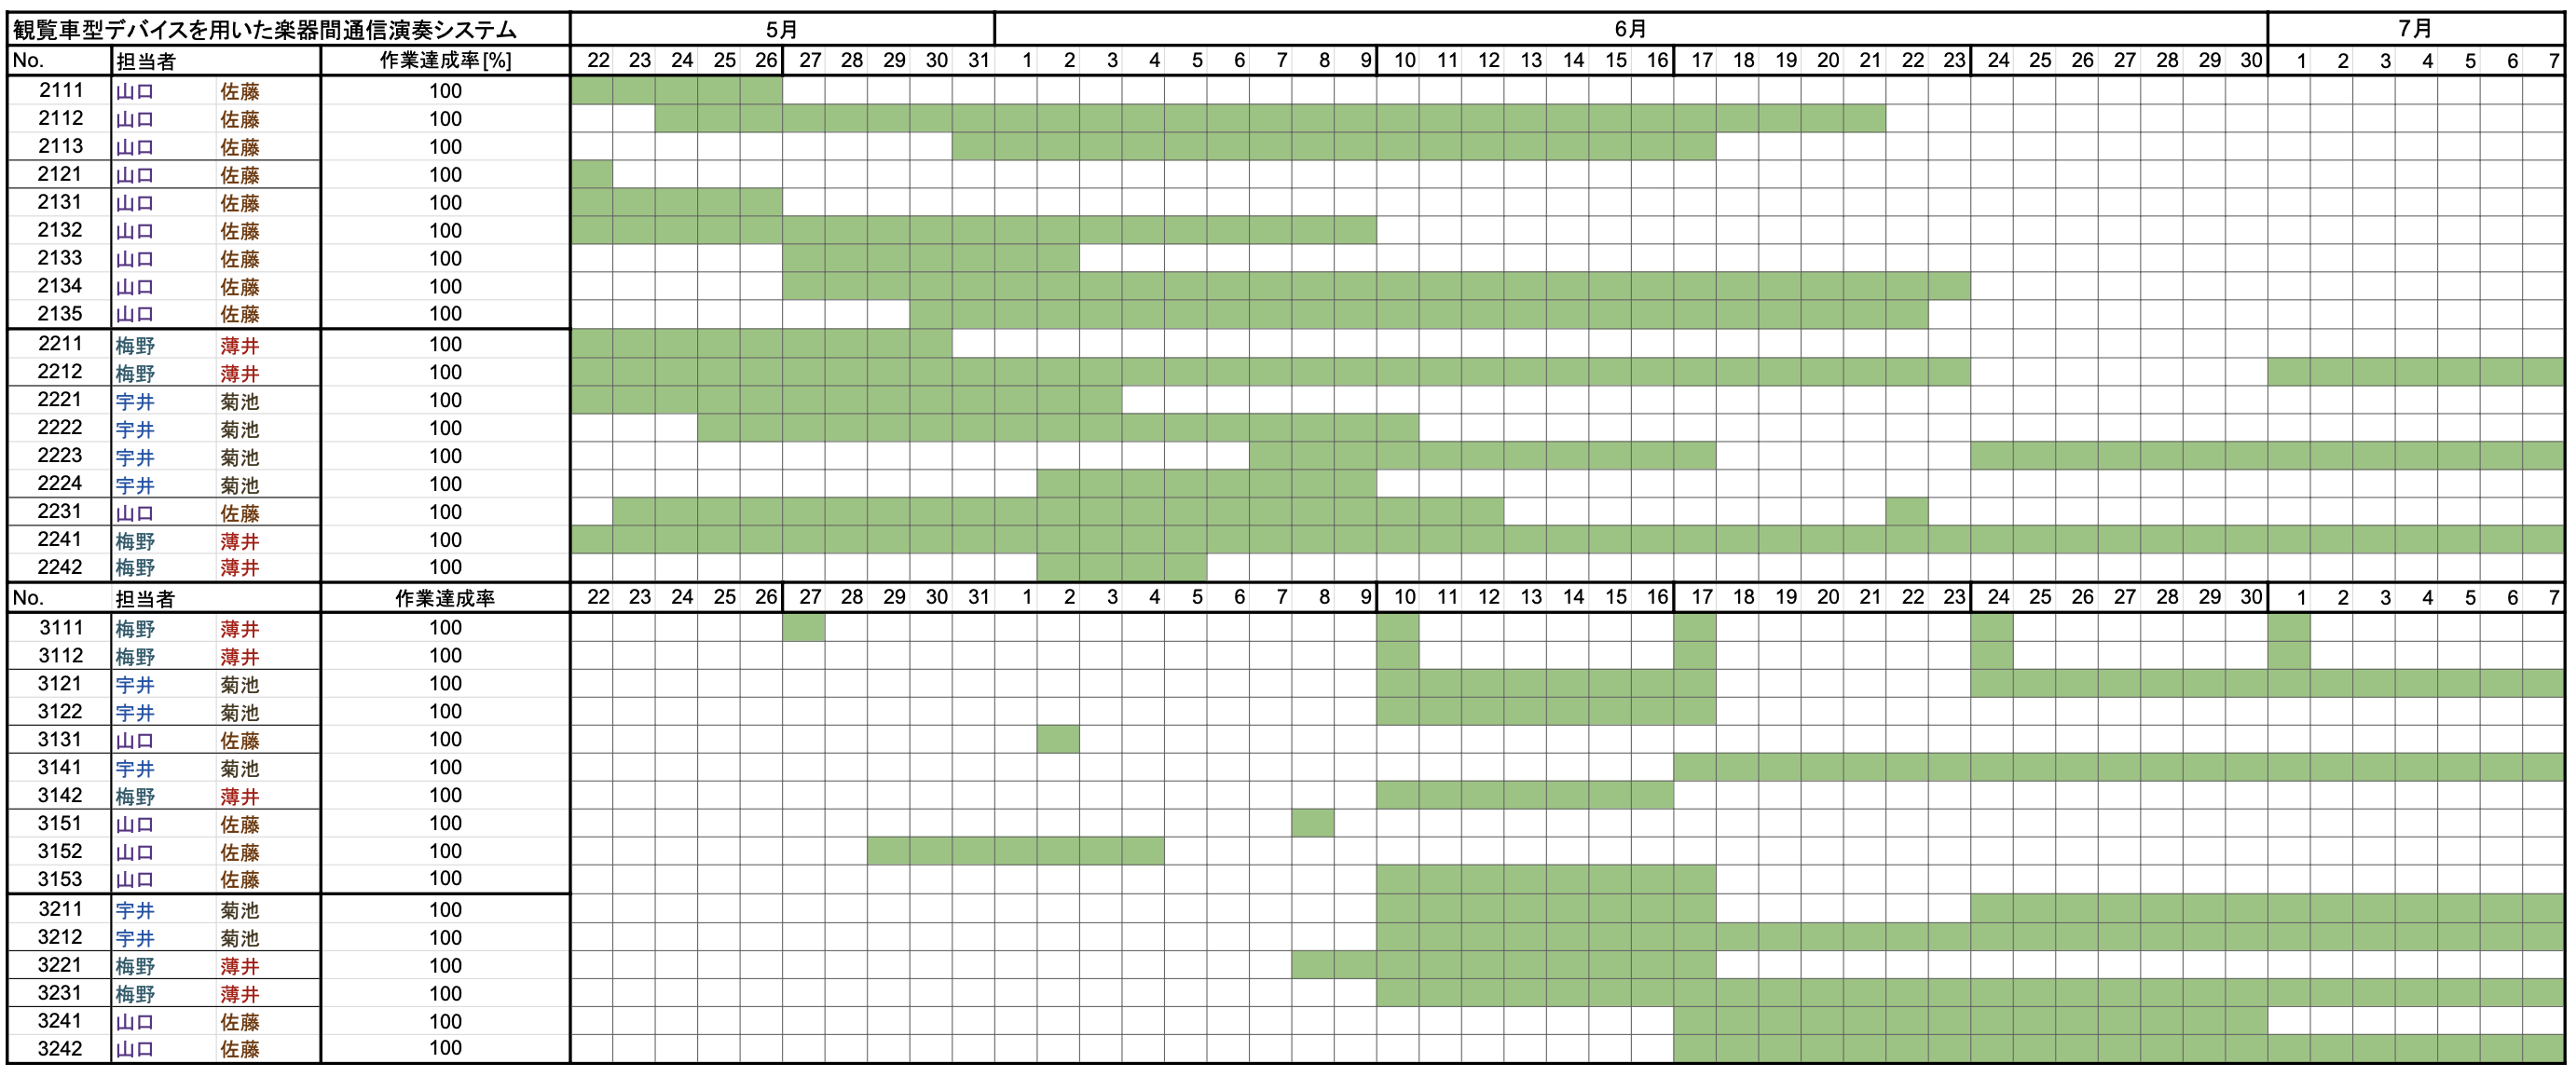
\includegraphics[width=\textwidth]{figs/GC_decide_goal.png}
    \caption{最終的な実績のガントチャート（上段：実装，下段：テスト）}
    \label{fig:gantt_final}
\end{figure}
\FloatBarrier

\subsection{報告者の担当範囲と技術的課題}
本節では，報告者が担当したハードウェアの実装について，採用した技術の選定理由を述べたうえで，実装の過程で直面した技術的課題とその解決のために行った技術的貢献を，各デバイスごとに説明する．
ハードウェア実装における共通の課題は，設計上は動作するはずの回路や機構を，実環境において安定して動作させることであった．具体的には，回転体の質量バランスや軸の摩擦といった機械的な問題，モータの特性変動といった電気的な問題，およびレーザー光の受光精度という光学的な問題が，実装段階ではじめて顕在化した．
以下では，これらの課題に対して行った対応を含めて述べる．


\FloatBarrier

\subsubsection{指揮デバイス}
\label{sec:jissou_siki}

はじめに，操作入力部品の選定理由について述べる．BPM・音量の調整には，スライド式可変抵抗器を採用した．回転式の可変抵抗器と比較して選定した理由は次の2点である．第一に，つまみの物理的な位置が設定値と対応するため，ユーザが現在のBPM・音量の段階を，表示装置を介さずつまみの位置のみから確認できるためである．
第二に，本デバイスは「指揮棒を振っている」というユーザの操作によって演奏が変化することで没入感を高めることが目的であり，回転式と比較してスライド式はデバイスを握ったまま親指のみで容易に操作が可能であり，演奏中に持ち替えを必要としないためである．
また，抵抗値には\SI{10}{\kilo\ohm}を選定した．これは，分圧回路としてArduinoのアナログ入力へ接続する際に，消費電流を抑えつつ，アナログ/デジタル変換の入力インピーダンスに対して十分に低い出力インピーダンスを保てる標準的な値である．

次に，振り動作の検知に用いる加速度センサの選定理由について述べる．振り動作の検知には，デジタル3軸加速度センサADXL345を採用した．選定理由は次の3点である．
第一に，3軸の加速度を同時に計測できるため，3軸のベクトル合成値を判定に用いることで，ユーザがデバイスを振る方向に依存しない検知を実現できる．第二に，このモジュールはI2C通信に対応しており，信号線2本（SDA・SCL）でArduinoと接続できるため，限られた実装空間における配線数を削減できる．第三に，測定レンジを$\pm 2g$から$\pm 16g$まで設定でき，振り動作で生じる加速度に対して測定値の飽和を避けた計測ができる．加えて，割り込み信号の出力ピン（INT1）を備えており，閾値超過の検知をセンサ側で行いArduinoへ通知する構成に対応できる．

次に，実装における技術的貢献について述べる．実装した指揮デバイスの内部を図\ref{fig:r_sikiin}に，外装を含む完成状態を図\ref{fig:r_siki}に示す．
内部は，ブレッドボード上にタクトスイッチと加速度センサを実装し，2系統のスライド式可変抵抗器はユニバーサル基板へはんだ付けして固定した．
外装の設計にあたっては，ユーザビリティの向上を目的として，ユーザが操作するスライド式可変抵抗器のスライダー部分およびタクトスイッチの部分を外装から露出させる構造とした．なお，本稿ではユーザが操作方法の説明を受けなくても，操作箇所を特定し目的の操作を行える度合いをユーザビリティと定義している．
これにより，ユーザは外装を開けることなく，露出したつまみとボタンのみで演奏の開始・終了とBPM・音量の全操作が行える．

\begin{figure}[htbp]
  \centering
  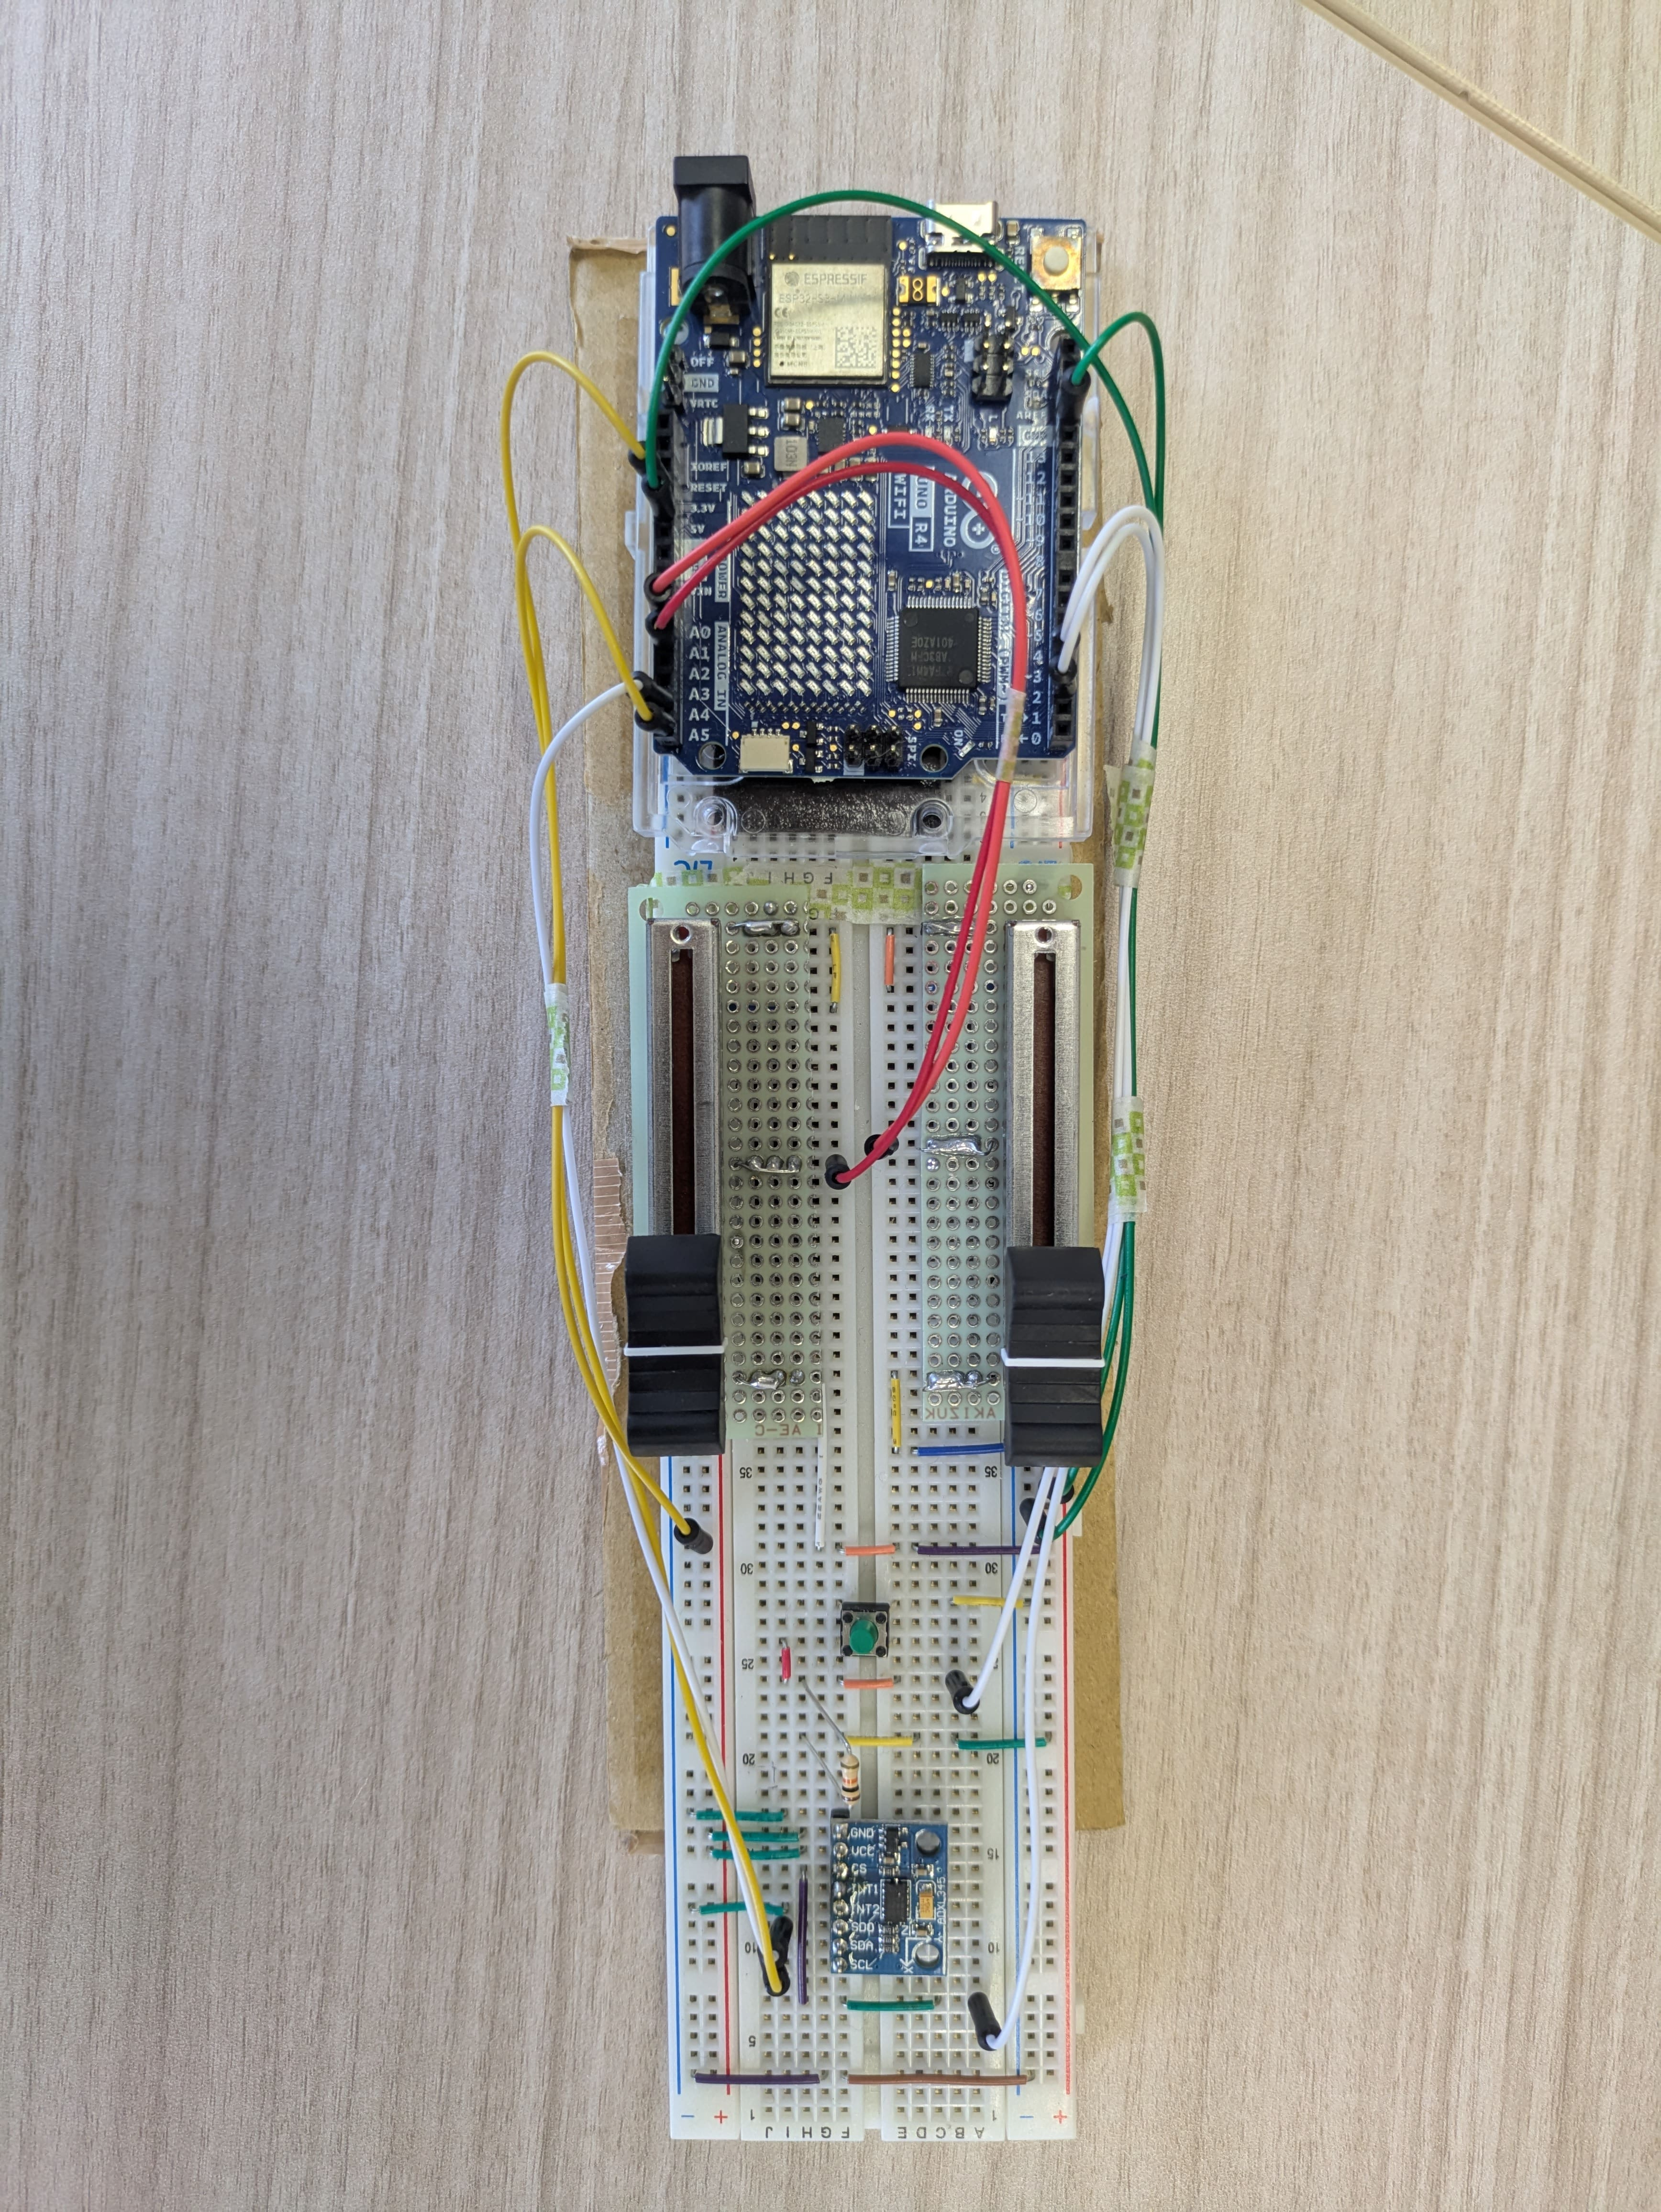
\includegraphics[width=0.55\textwidth]{figs/R_sikiin.jpg}
  \caption{指揮デバイスの内部実装}
  \label{fig:r_sikiin}
\end{figure}

\begin{figure}[htbp]
  \centering
  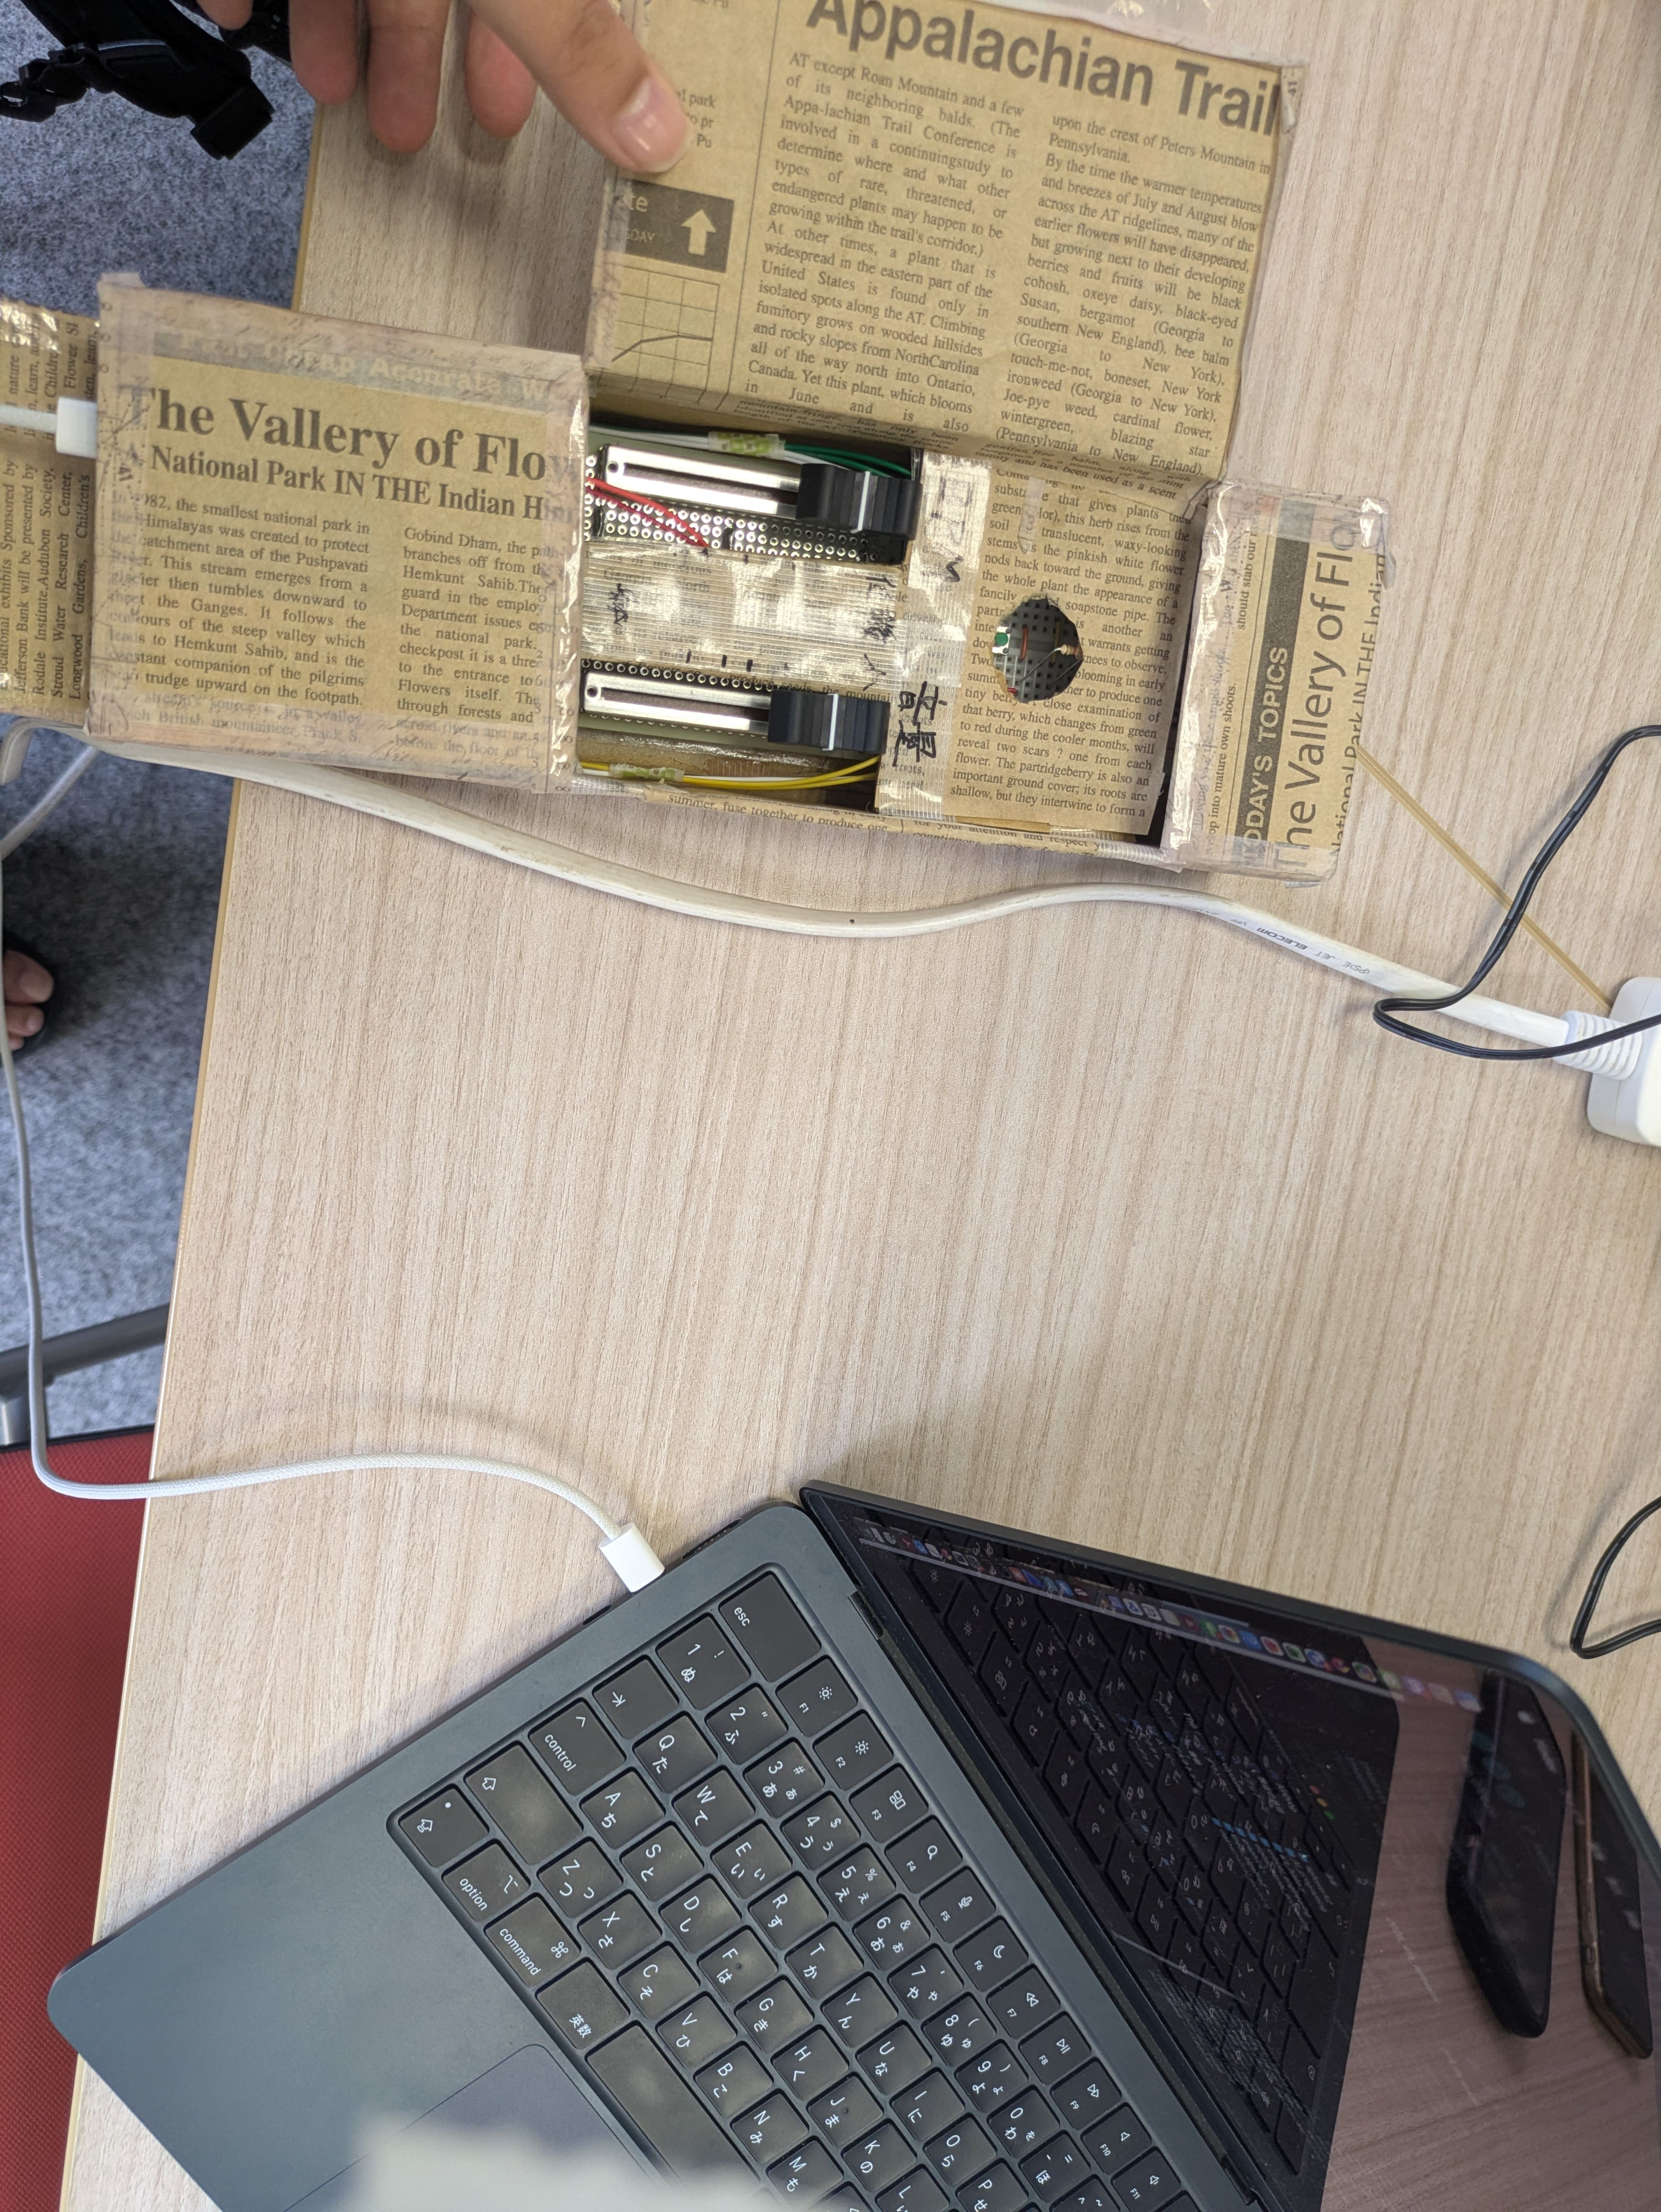
\includegraphics[width=0.7\textwidth]{figs/R_siki.jpg}
  \caption{作成した指揮デバイス}
  \label{fig:r_siki}
\end{figure}

\FloatBarrier



\subsubsection{観覧車型中継機デバイス}
\label{sec:jissou_kan}

はじめに，主要部品の選定理由について述べる．
第一に，回転リング上のレーザーモジュールの電源には，ボタン電池を採用した．
レーザーモジュールは回転リングに搭載されて本体ごと回転するため，外部から配線で給電すると回転に伴い配線が捻れ，回転体へ電力を伝えるための回転接点部品であるスリップリング等の追加機構が必要となる．
そこで，電源を回転体上で完結させる方式とし，回転体に搭載する電源として小型・軽量で質量バランスへの影響が小さいボタン電池を選定した．型番には，ボタン電池の中でも大容量なCR2477を選定した．採用したレーザーモジュールは\SI{3}{V}駆動かつ定電流回路を内蔵しているため，公称電圧\SI{3}{V}で外部抵抗なしに直結でき，回路を簡素化できる\cite{laser}．また，基板取付用ホルダーを介して実装することで，電池の消耗時に交換が可能である．
実際に作成したレーザーによる光信号送信基盤を図\ref{fig:laser_kiban}に示す．図\ref{fig:laser_kiban}の通り，ユニバーサル基盤にボタン電池ホルダとレーザーモジュールをはんだ付けしている．これにより，ボタンをオンにすると回転リングの穴からレーザー光が照射される．

第二に，モータの駆動には，モータドライバモジュールを採用した．Arduinoのデジタル出力ピンはモータの駆動に必要な電流を直接供給できないため，Arduinoからモータへ電力を供給するためのモータドライバが必要となる．DRV8835を選定した理由は次の3点である．
第一に，Hブリッジという4つのスイッチング素子を組み合わせ，モータへ流す電流の向きを切り替えられる回路を内蔵し，PWM信号の入力によって回転速度の制御が可能であるからだ．第二に，モータ用電源として最大\SI{11}{V}・1チャネルあたり最大\SI{1.5}{A}の駆動に対応しており，ACアダプタからの\SI{5}{V}単一電源系でギヤボックスモータを駆動できる．第三に，ブレッドボードに直接実装できる小型のDIP化モジュールであり，試作段階においてはんだ付けを行わずに配線を変更できる．実装したモータドライバ周辺の回路を図\ref{fig:r_mota}に示す．

\begin{figure}[htbp]
    \centering
    \includegraphics[width=0.6\textwidth]{figs/R_laser.jpg}
    \caption{実際に作成したレーザーによる光信号送信基盤}
    \label{fig:laser_kiban}
\end{figure}



\begin{figure}[htbp]
  \centering
  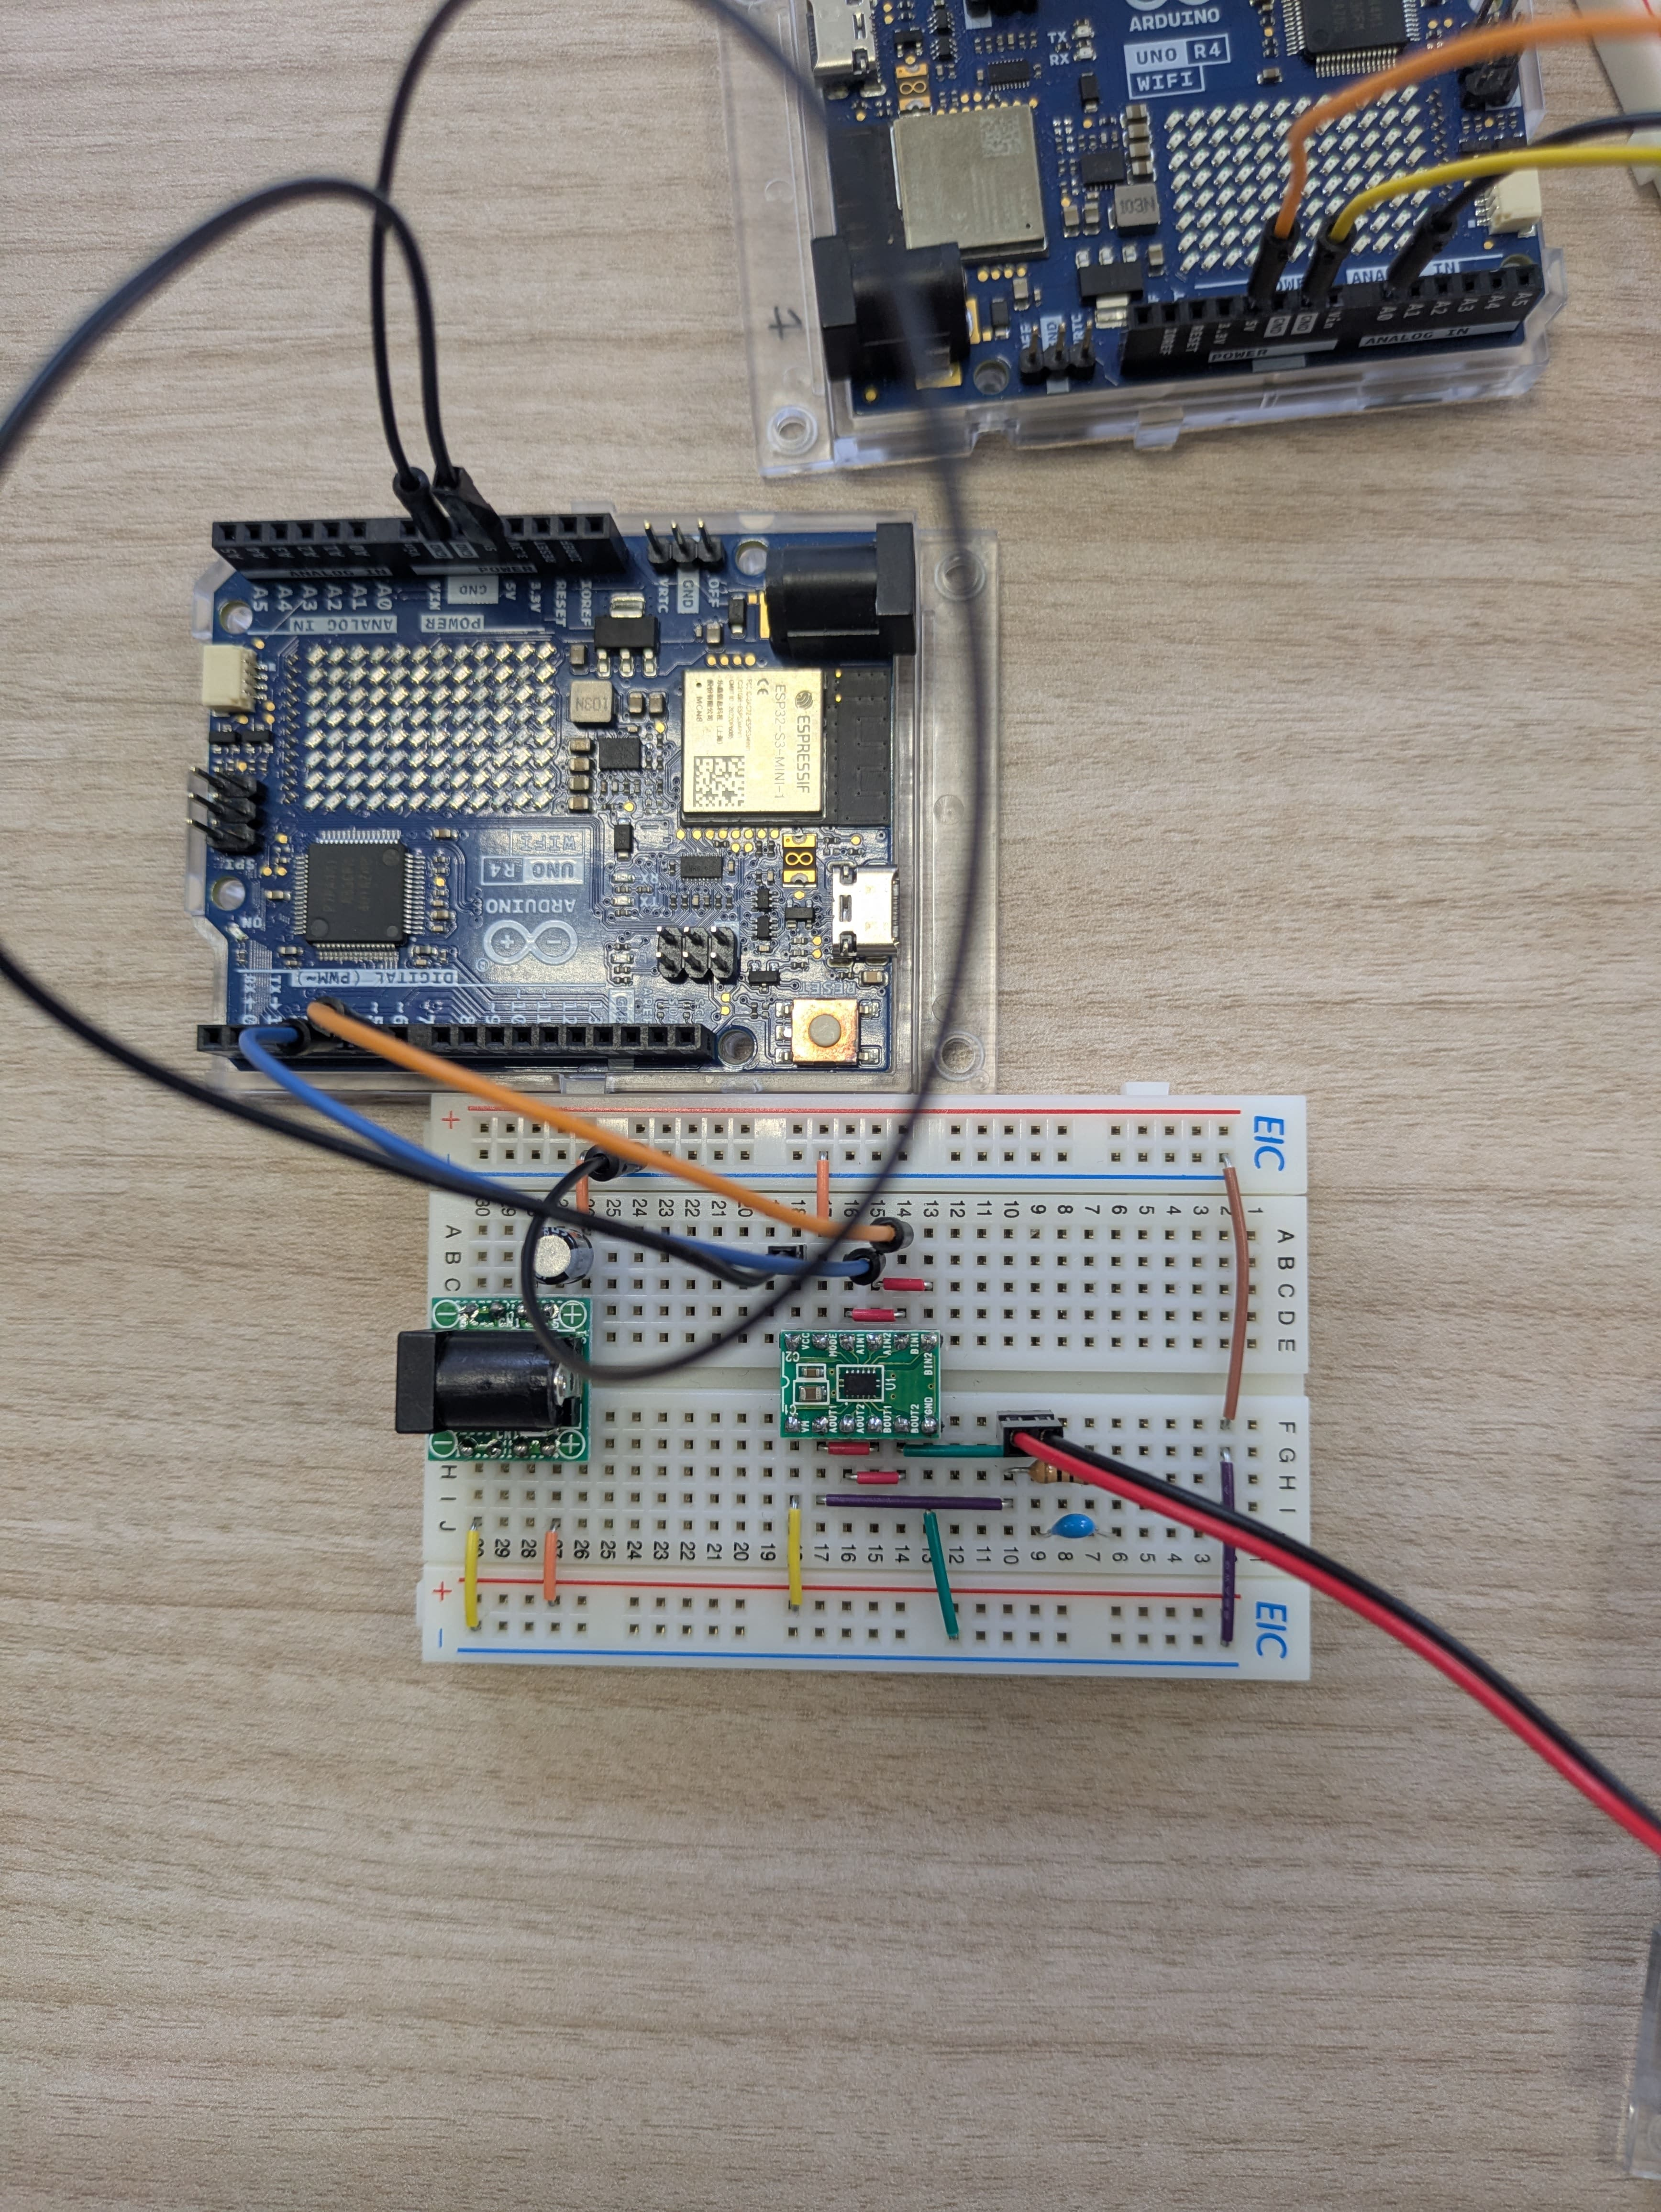
\includegraphics[width=0.6\textwidth]{figs/R_mota.jpg}
  \caption{モータドライバ周辺の回路実装}
  \label{fig:r_mota}
\end{figure}

次に，実装における技術的貢献について説明する．実装した中継機デバイスの全体を図\ref{fig:r_zentai}に示す．

\begin{figure}[htbp]
  \centering
  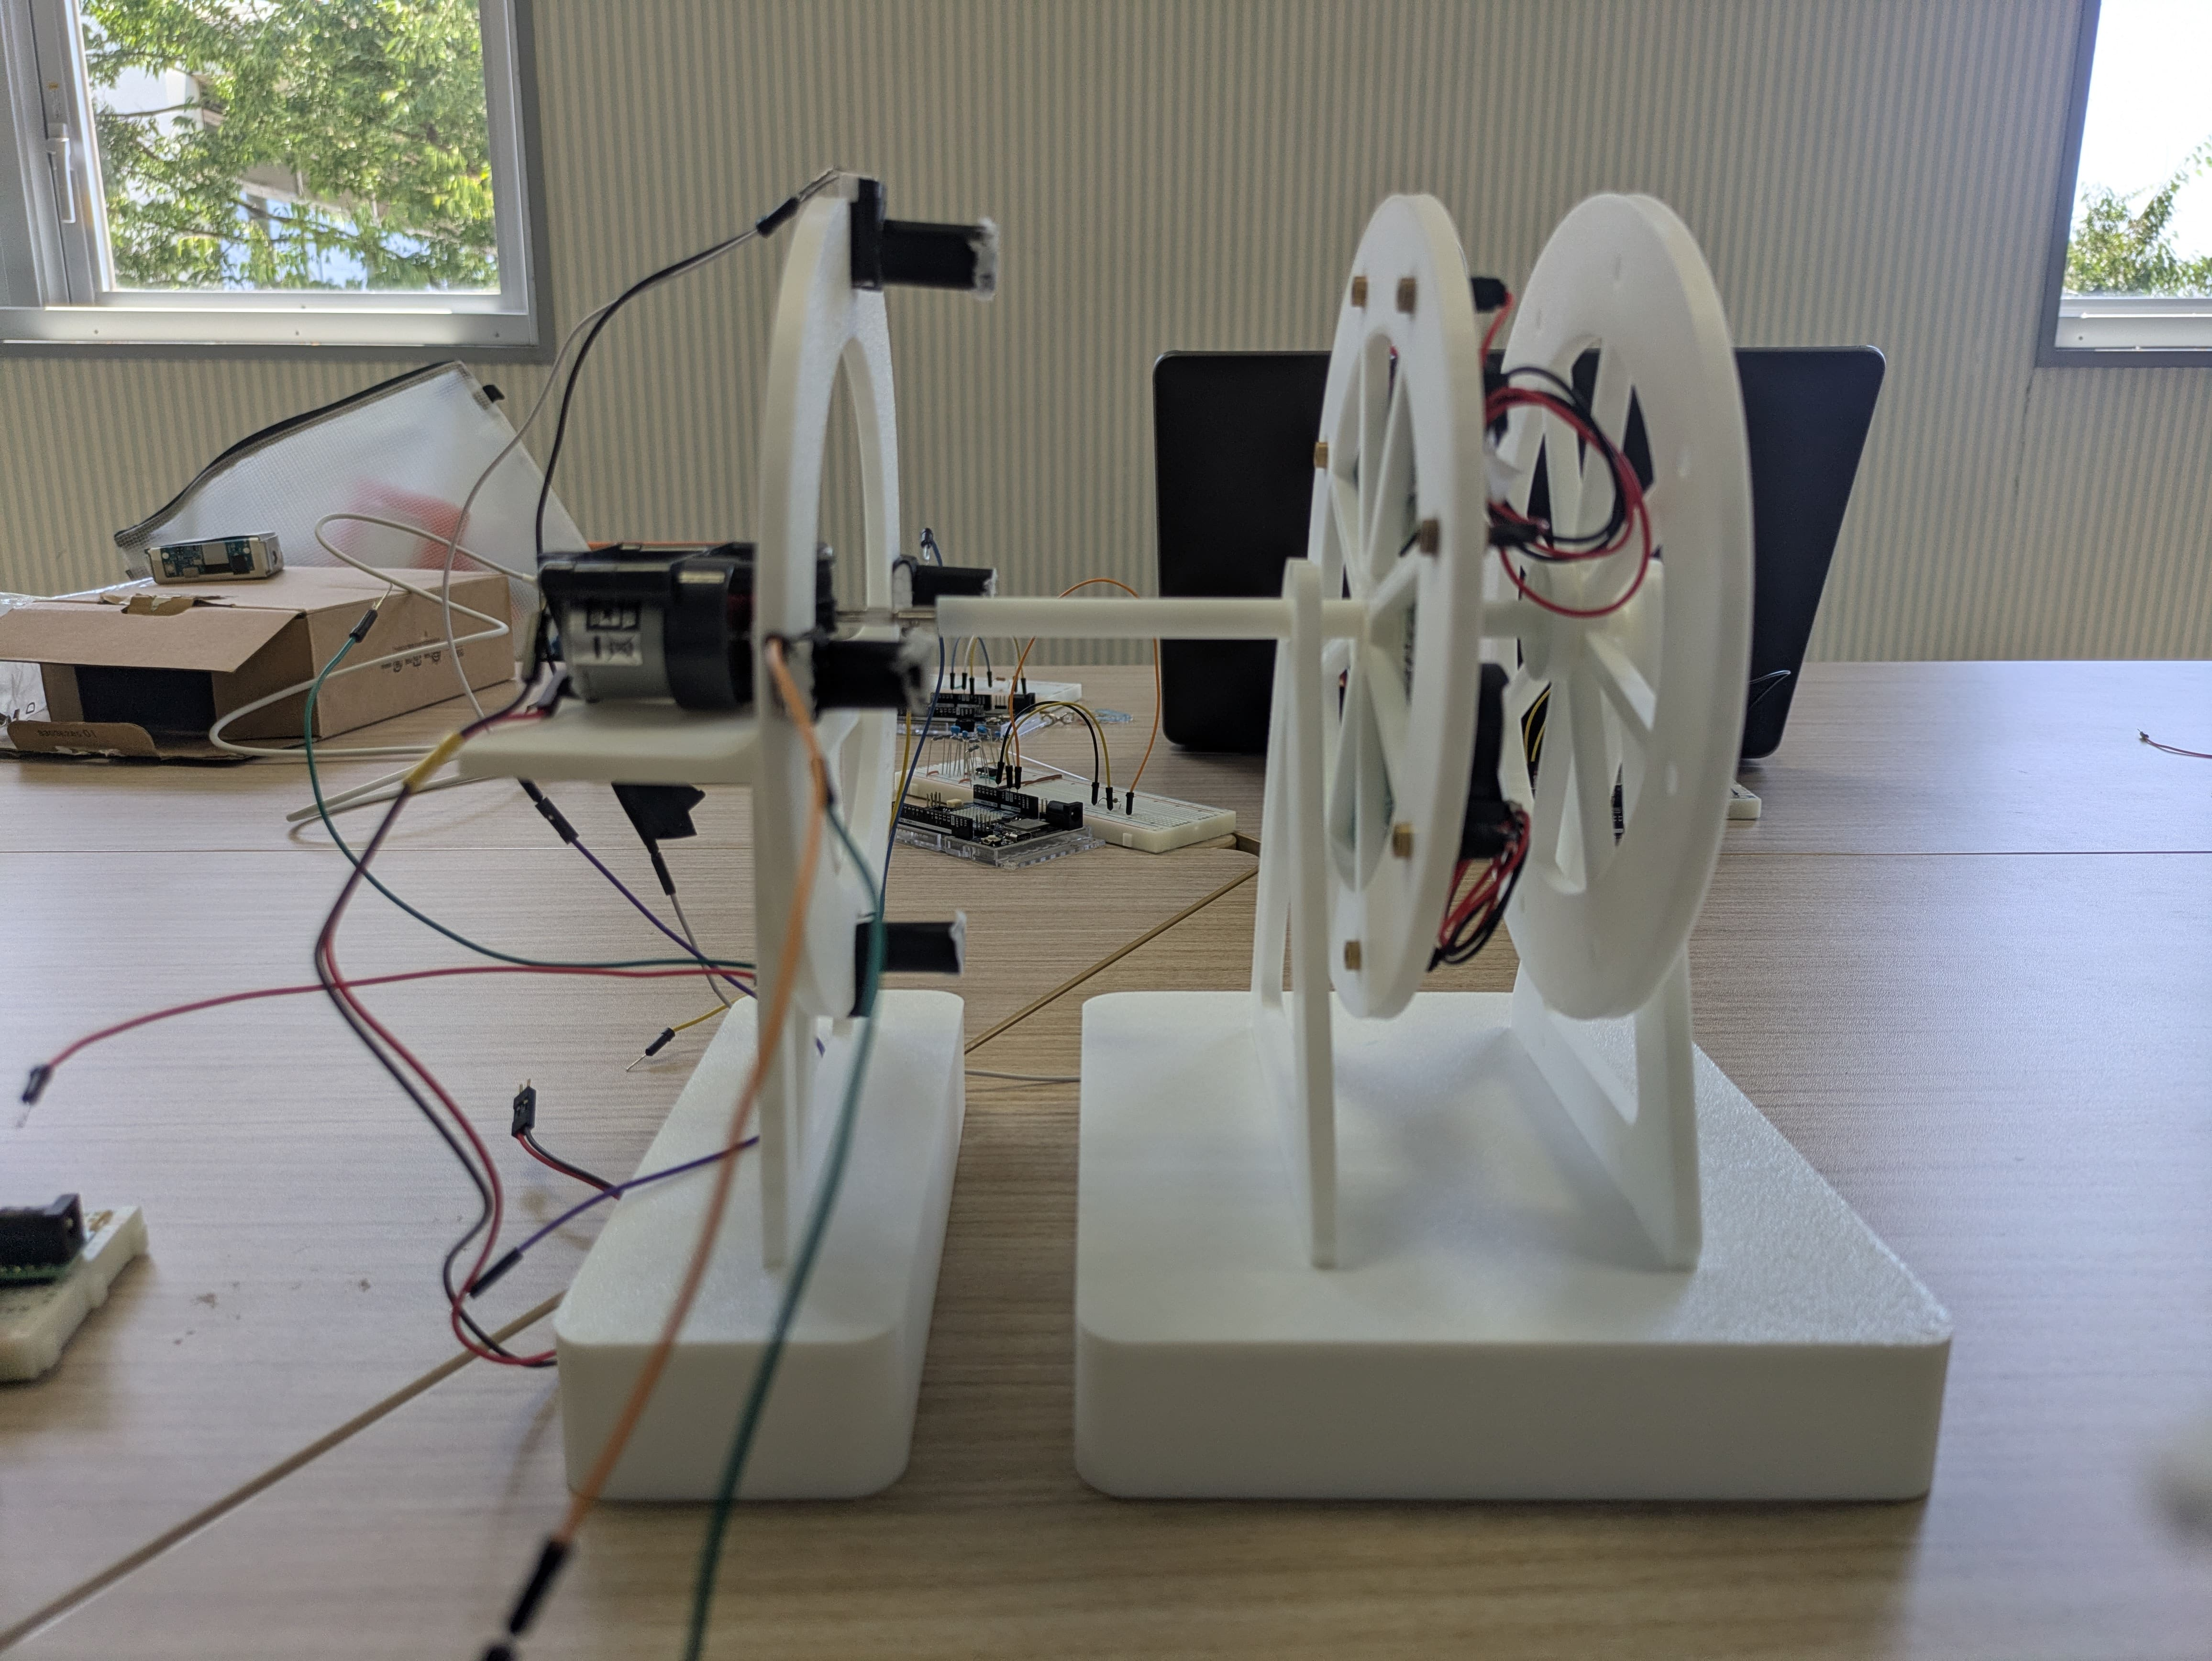
\includegraphics[width=0.8\textwidth]{figs/R_zentai.jpg}
  \caption{実装した中継機デバイスの全体（左：受光部リング側，右：回転リング側）}
  \label{fig:r_zentai}
\end{figure}

\noindent
まず，回転部の機械的な安定化について述べる．回転する部品を支える回転軸は，安定性を担保するために左右の支柱で軸受け穴の大きさを非対称とし，ギヤボックスモータに接続する側の穴を大きくしている．これは，モータ側の軸受けに回転トルクによる負荷が集中し，穴の径が小さいと軸が折れるおそれがあるためである．
軸まわりの部品形状を図\ref{kanran2}，図\ref{kanran3}に示す．計画書当初は同一の大きさに軸を設計しており，実際に3Dプリンターにて実装をしたところ耐久性に乏しく折れてしまったが，現在の仕様に変更したところ実験中に軸が折れることはなく，安定性が担保された．
さらに，軸受け部にはグリス（半固体状の潤滑剤）を塗布し，軸と軸受け間の摩擦を低減させた．また，回転軸をモータへ差し込む接続部にはネジロック剤（振動による締結部の緩みを防止する接着剤）を塗布し，回転の振動による軸の緩み・脱落を防止した．

% \begin{figure}[htbp]
%   \centering
%   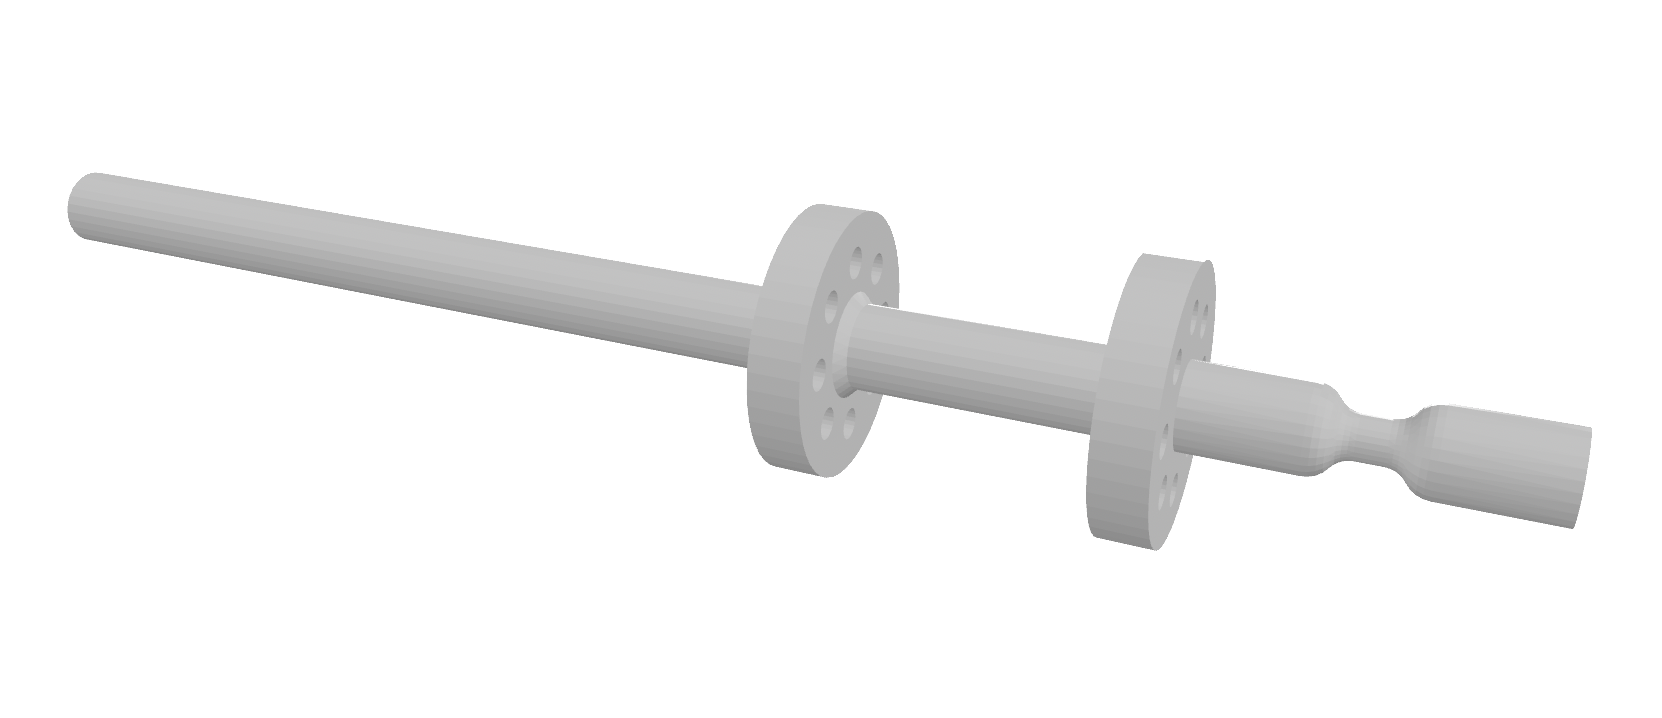
\includegraphics[width=0.45\textwidth]{figs/model_shaft.png}
%   \caption{回転軸部の形状（3Dモデルデータ）}
%   \label{fig:jiku_daiyou}
% \end{figure}

% \begin{figure}[htbp]
%     \centering
%     \centering
%     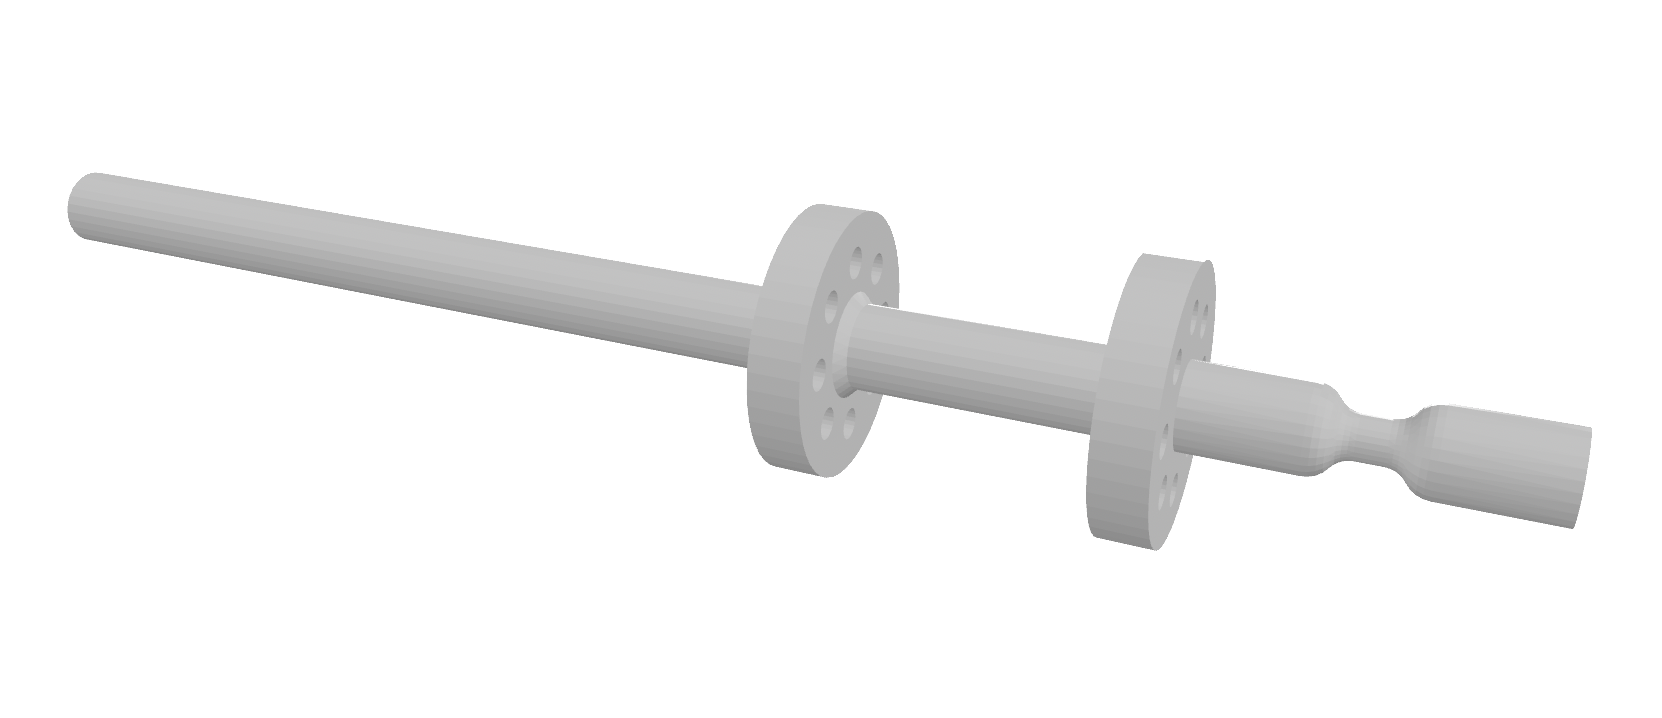
\includegraphics[width=5cm]{./figs/model_shaft.png}
%     \caption{設計に使用するモデルデータ(回転軸部)}
%     \label{kanran3}
% \end{figure}


次に，回転体の質量バランスの調整について述べる．ボタン，電池，ホルダー，そしてレーザーモジュールで構成される，レーザーによる光信号送信基盤を回転リングへ取り付ける際，当初はリング内に収まることを優先して両面テープで貼り付けていた．
しかし，この配置では回転体の質量分布に偏りが生じ，回転速度にムラが発生した．そこで，4枚の電池基板を中心軸を囲うように十字状の対称配置へ変更することで偏心を抑え，回転速度のムラを解消した．さらに，両面テープでは回転の振動により固定が緩むため，瞬間接着剤による固定へ変更し，安定性を向上させた．実装した回転リングの表面・裏面を図\ref{fig:r_kanran}に示す．

\begin{figure}[htbp]
  \centering
  \begin{minipage}{0.48\textwidth}
    \centering
    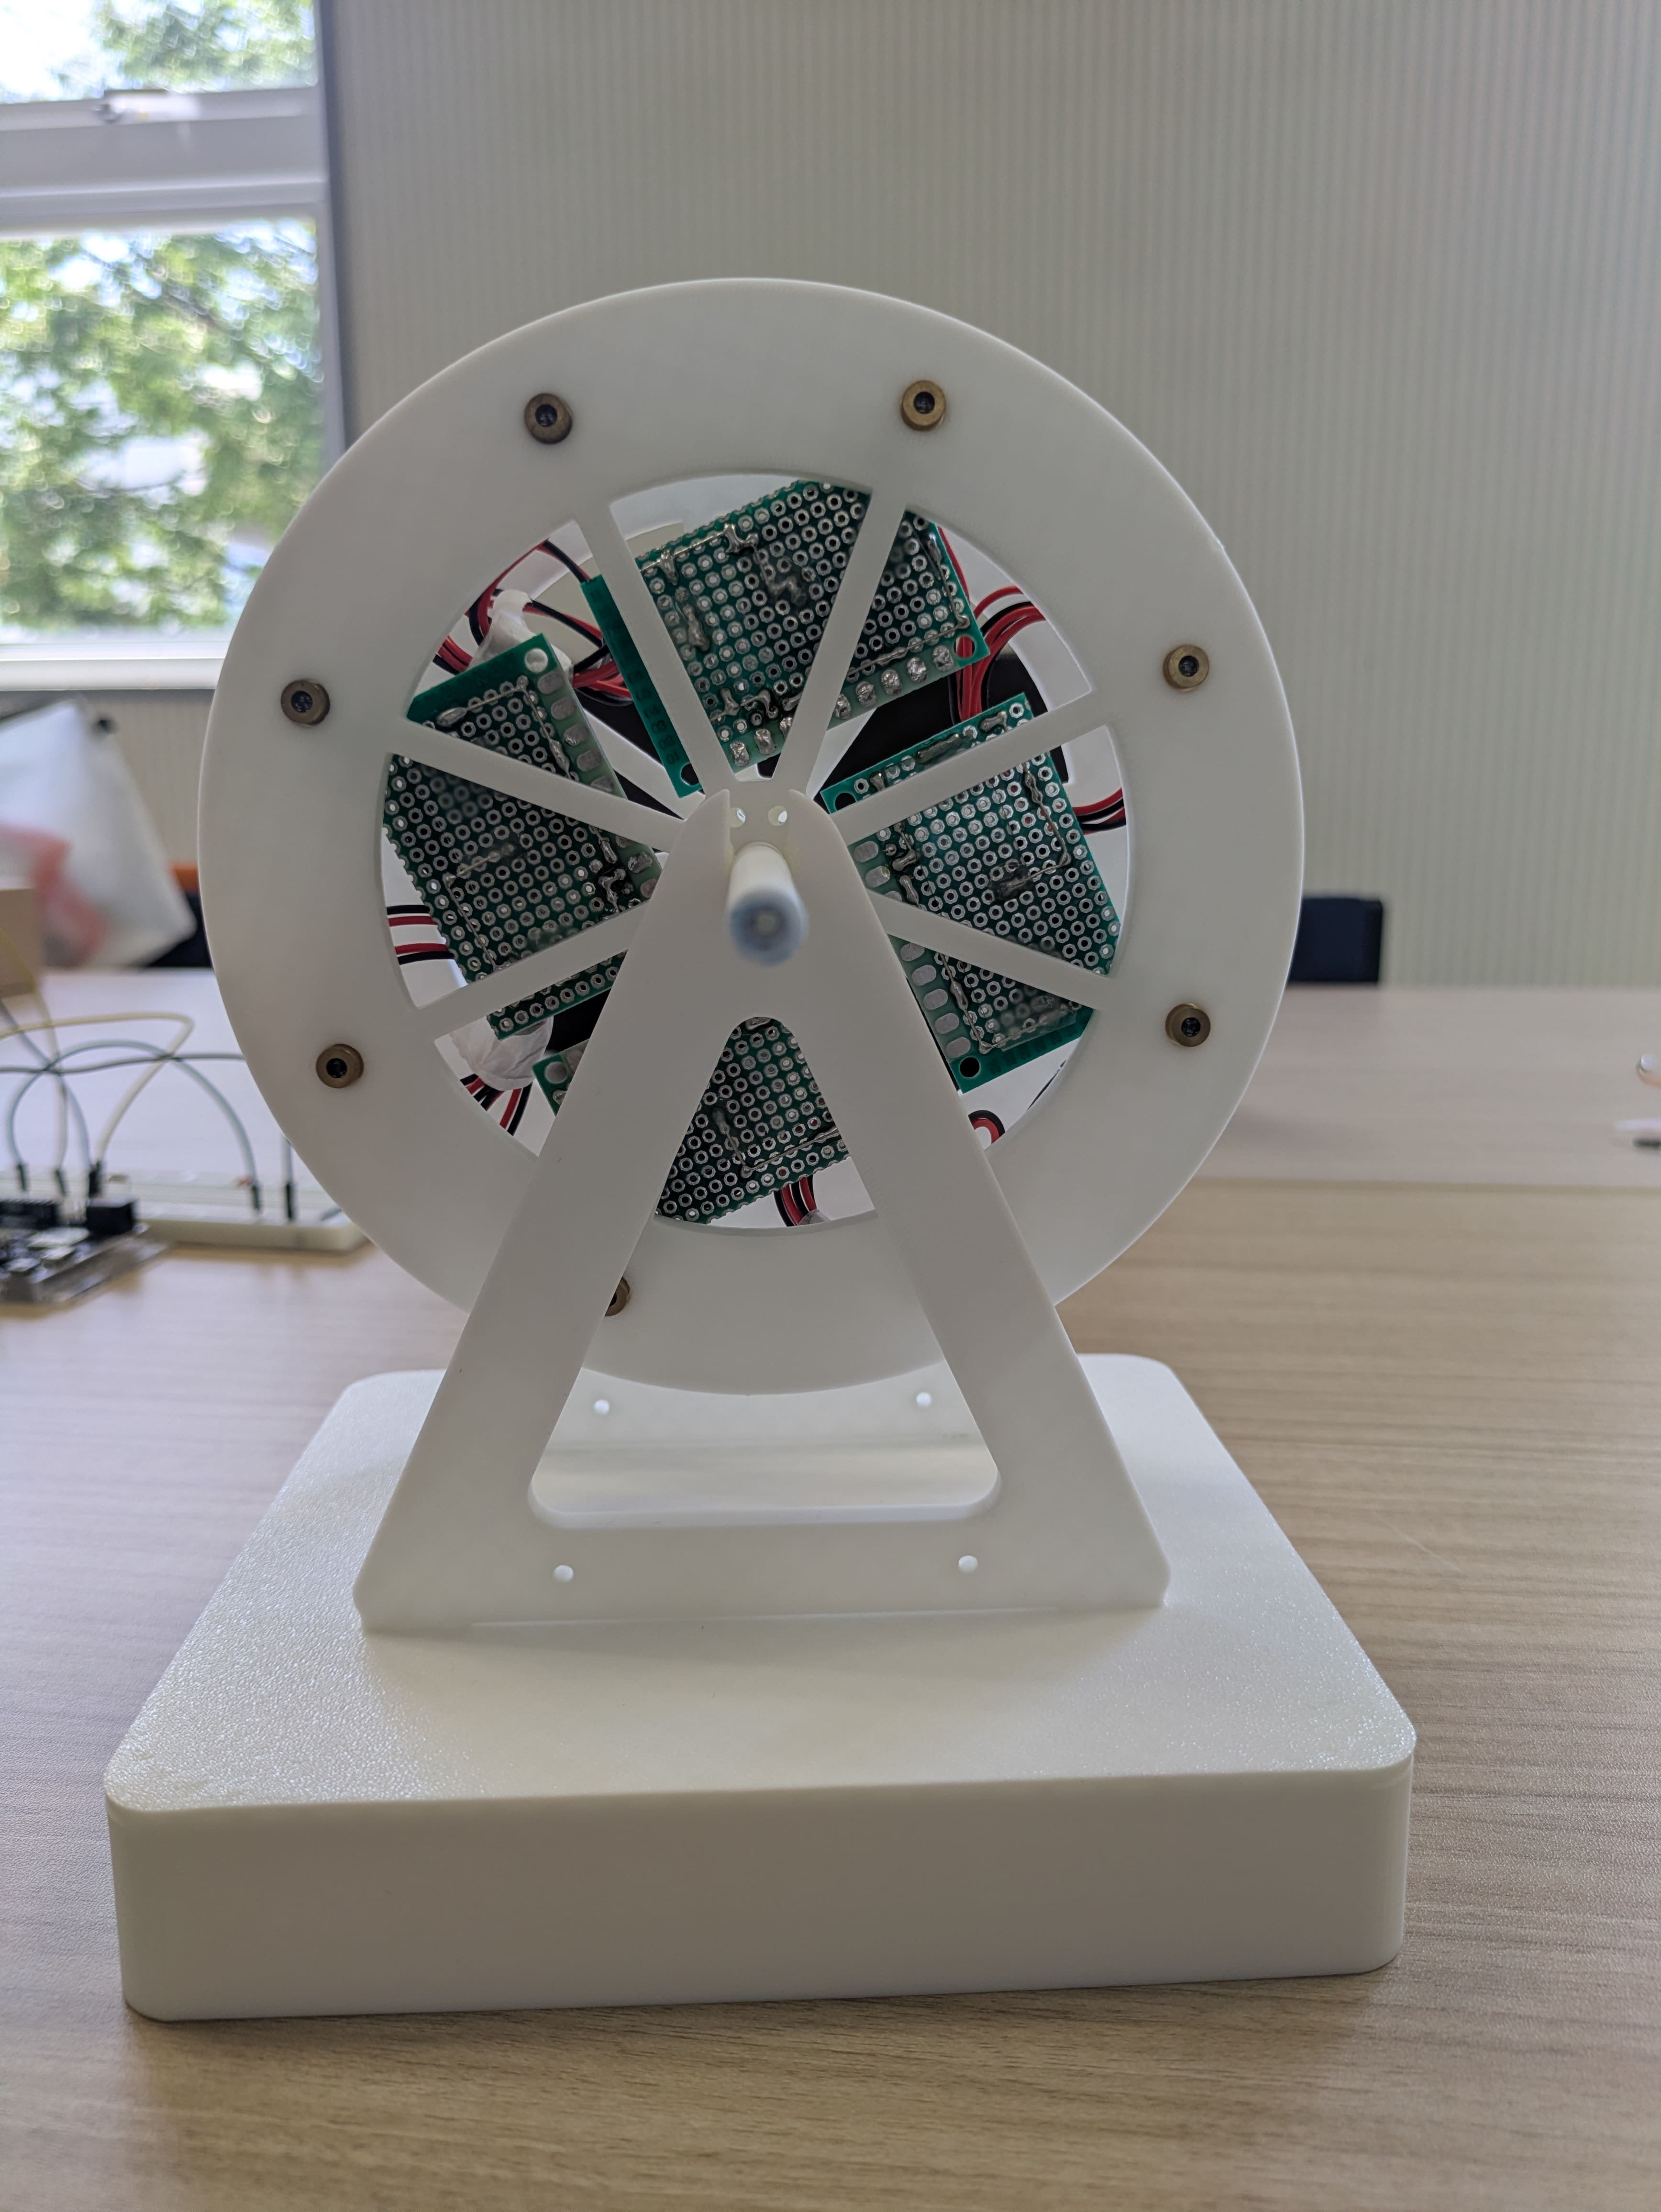
\includegraphics[width=\textwidth]{figs/R_kanranomote.jpg}
  \end{minipage}
  \hfill
  \begin{minipage}{0.48\textwidth}
    \centering
    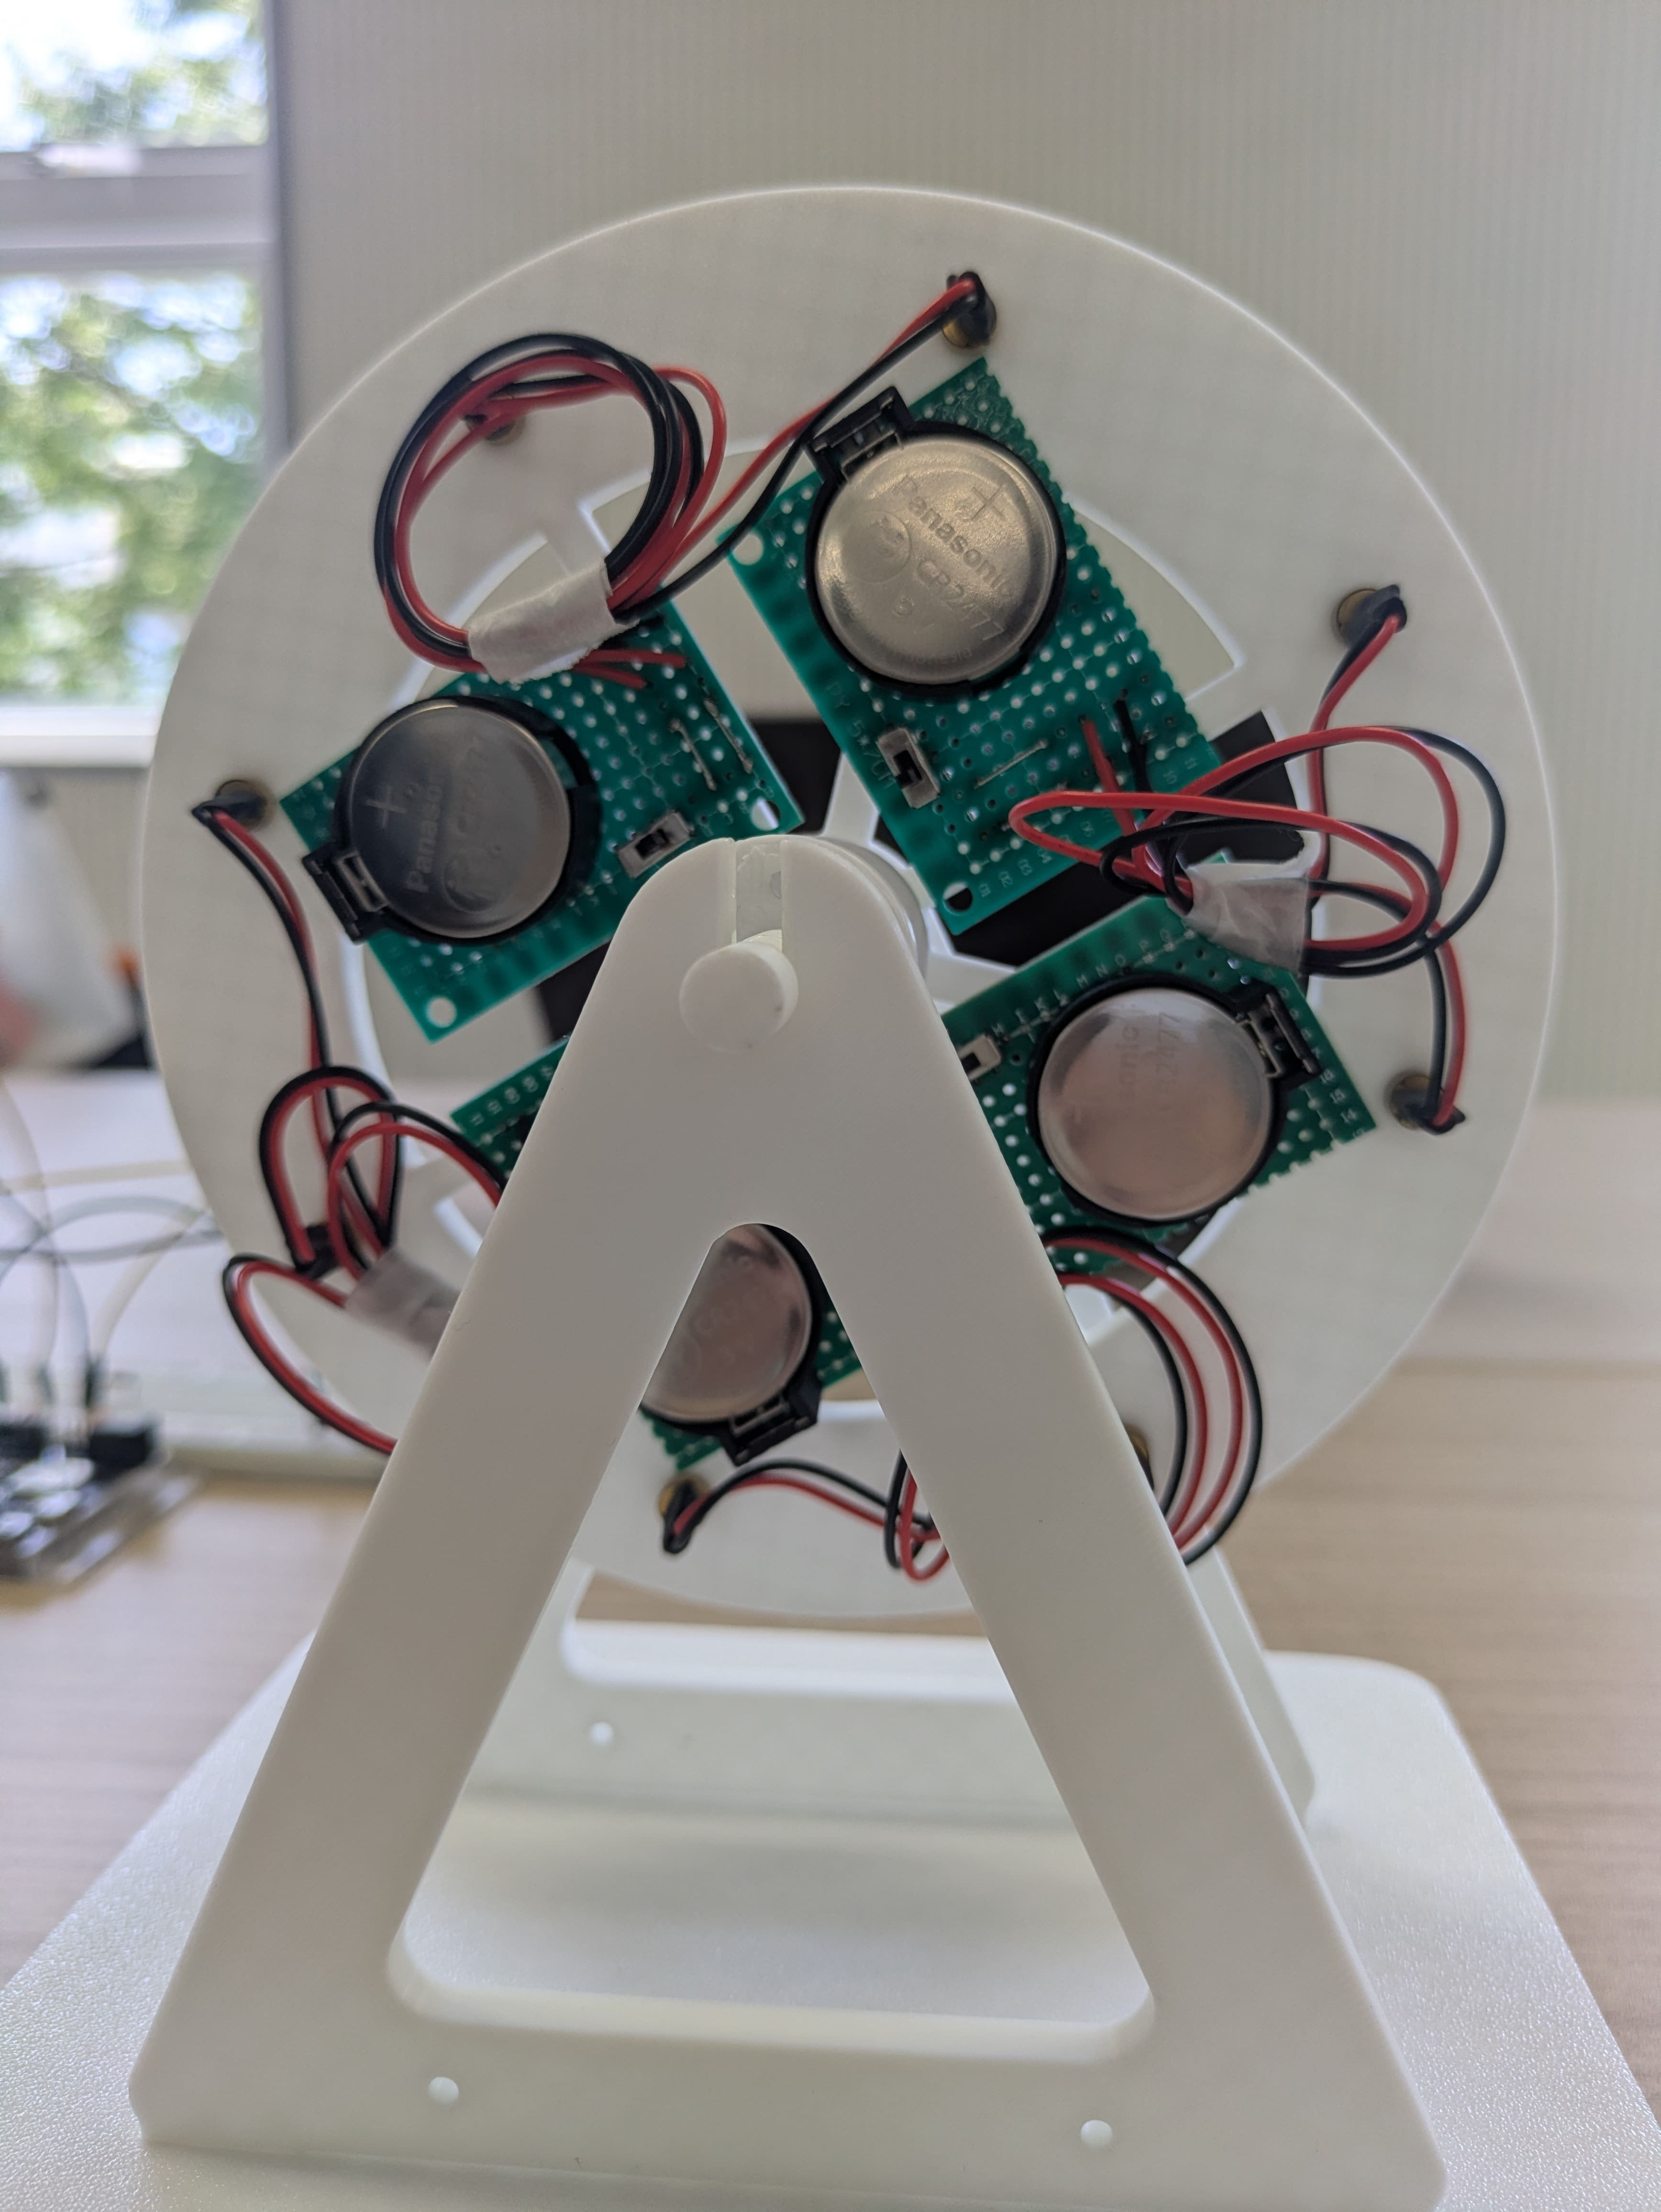
\includegraphics[width=\textwidth]{figs/R_kanranura.jpg}
  \end{minipage}
  \caption{回転リングへのレーザーによる光信号送信基板の実装（左：正面，右：背面）}
  \label{fig:r_kanran}
\end{figure}


また，動作試験の過程で，回転の反動によりモータ部が土台から浮いて動いてしまい，レーザー光の照射位置がずれて受光精度が低下する事象が確認された．この対策として，使用済みのボタン電池を土台部に載せておもりとし，モータ部の浮き上がりを抑えた．廃棄予定の電池を再利用することで，追加部品なしに質量を確保している．

さらに，動作試験を繰り返す中で，同一のPWM設定値に対するモータの回転速度が試行ごとに一定にならない事象が確認された．この要因としては，電源の起電力が試行ごとに変動していたことが考えられる．
モータの回転速度は印加電圧に依存するため，電源電圧の変動やブラシ接触抵抗の変化が回転速度の変動として現れたと考えられ，\ref{sec:kousatsu}節で述べる同期確立時間の変動要因の一つとなった可能性がある．

% 最後に，本デバイスのモータ回転制御およびLEDマトリクス表示を行う制御プログラムの全文は，付録（FerrisWheel.ino，Display.h，Display.cpp，MotorControl.h，MotorControl.cpp）に示す．

\FloatBarrier

\subsubsection{楽器デバイス受光部装置}
\label{sec:jissou_jukou}

はじめに，受光素子の選定理由について述べる．
レーザー光の検知にはCdSセルを採用した．CdSセルとは，硫化カドミウムを用いた，受光量に応じて抵抗値が変化する光導電素子である．
CdSセルは，フォトダイオード等の他の受光素子と比較して応答速度は遅いものの，抵抗値の変化を分圧回路で読み取るだけの簡素な回路で使用でき，可視光域に感度を持つためレーザーモジュール（波長\SI{650}{nm}の赤色光）の検知に適する．
本システムの受光イベントは最低でも数百 m秒であるモータの回転周期で発生するため，CdSセルの応答速度で十分であると判断した．

次に，実装における技術的貢献について述べる．
まず，レーザー光を使用する際における安全対策について述べる．レーザー光は直接目に入ると危険であるため，回転する部品と同じ大きさの阻害部品（遮光板）を製作し，レーザー光が受光部の後方へ漏れて観客の目に入ることを防止した．受光部の円盤形状は図\ref{kanran6}に示す通りである．

% \begin{figure}[htbp]
%   \centering
%   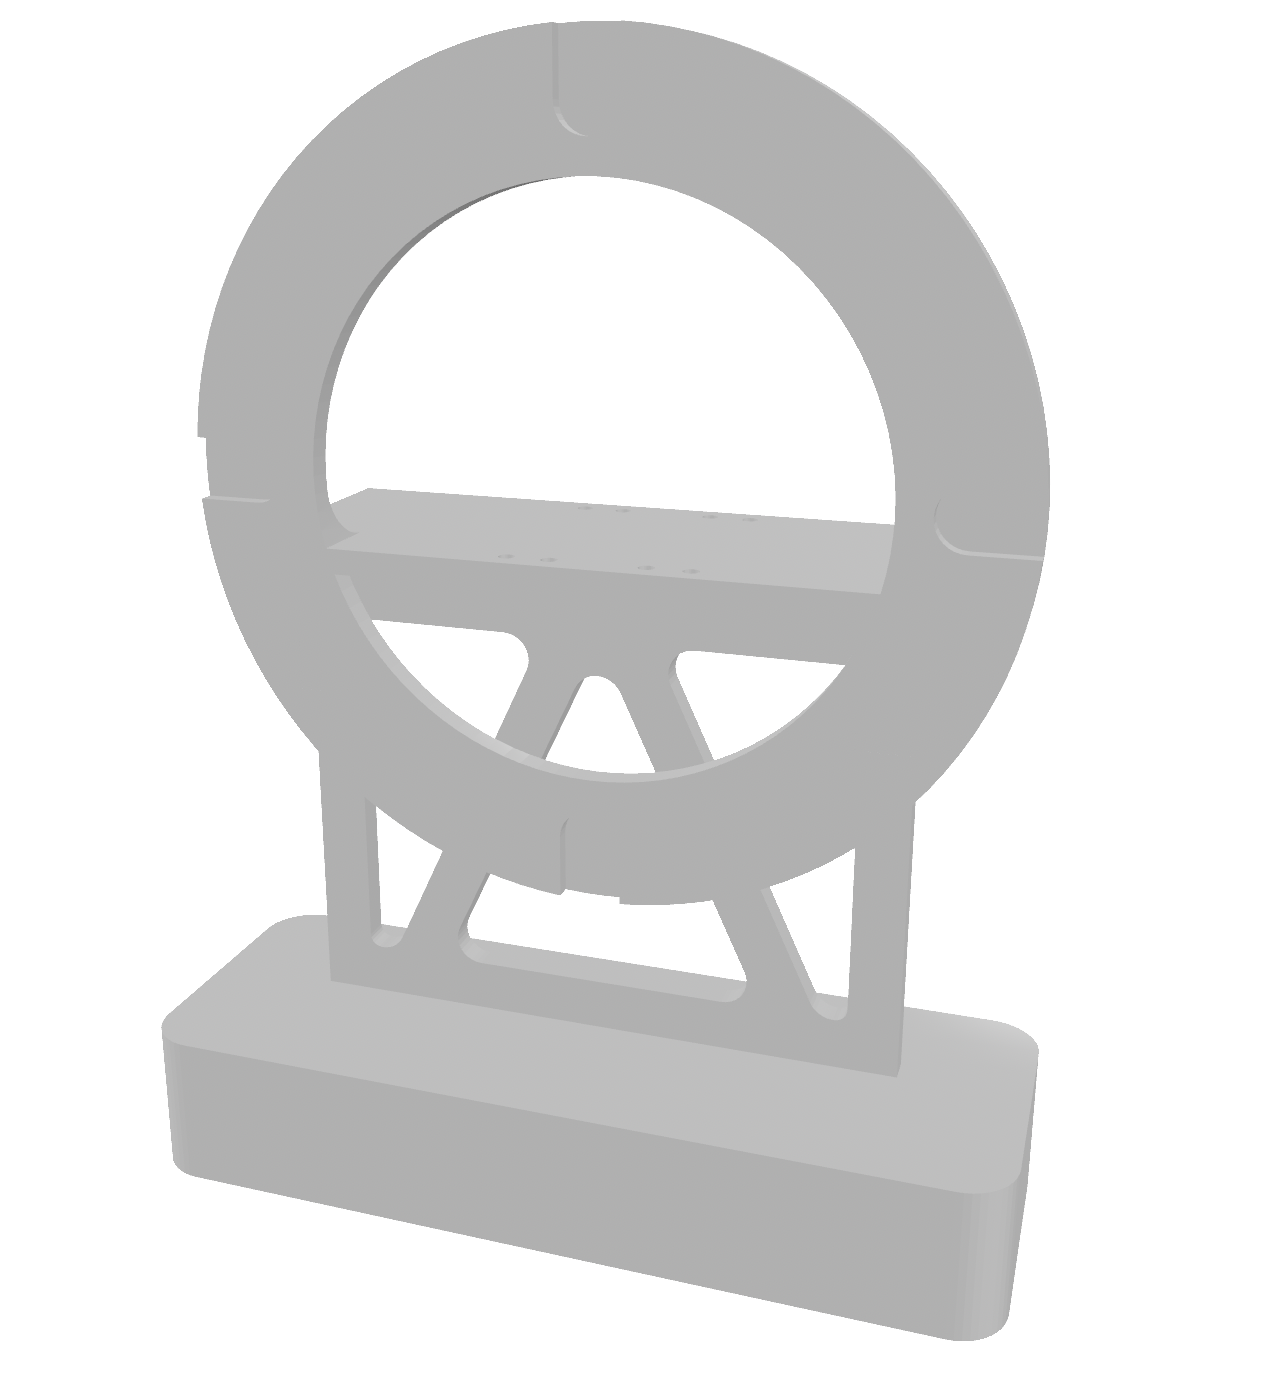
\includegraphics[width=0.45\textwidth]{figs/model_pointer.png}
%   \caption{受光部円盤の形状（3Dモデルデータ）}
%   \label{fig:jukou_daiyou}
% \end{figure}
\noindent
次に，CdSセルの設置方法について述べる．受光部の遮光板には，図\ref{kanran6}の通りCdSセルを設置するためのくぼみを90度間隔に設けている．CdSセルをこの受光部の遮光板へ固定するにあたり，当初はCdSセルを遮光板へ直接固定することを検討したが，デバイスの組み立て方やレーザー光の機微な方向の違いによって受光しやすい位置が変わり受光精度が変動するという問題があった．また，本デバイスは3Dプリンターで制作したため，ポリ乳酸(PLA)という素材特性の観点からも設置が困難である．PLAは硬度が高く寸法安定性に優れる一方で，表面が滑らかで接着剤が定着しにくいという特性を持つ．以上の観点から，CdSセルを遮光板に直接接着した場合，十分な固定強度が得られず受光精度が不安定となる問題があった．
そこで，小さく切った発泡スチロールにCdSセルの素子部分を折り曲げて沿わせ，テープで固定したうえで，この発泡スチロールごとくぼみに設置する方式とした．これにより，発泡スチロールを動かすことでCdSセルの位置を微調整でき，組み立て後にレーザー光の照射位置へ合わせ込むことが可能となった．なお，この方式で実験を続けたところ，固定していたテープが浮いてしまう事象が生じたため，テープの重ね貼りによる補強を行った．





最後に，受光精度の向上について述べる．CdSセルは受光面が小さく，回転するレーザー光の細いビームを直接受光することが困難であったため，受光精度を段階的に改善した．
まず，黒いストローでCdSセルを覆った．これは，ストローの筒内に入射したレーザー光が内部で反射してCdSセルへ届きやすくなるとともに，筒が周囲の環境光を遮ることで，受光時と非受光時の明暗差を大きくする狙いである．しかし，一般的な細さのストローでは開口部が小さく，依然として受光が困難であったため，開口径の大きいタピオカ用の黒いストローへ変更したところ，受光精度が向上した．
さらに，ストローの先端をティッシュペーパーで薄く覆うことで，レーザー光が通過する際に拡散され，ビームの位置が多少ずれても拡散光としてCdSセルへ届くようにした．加えて，ストローとCdSセルの間を瞬間接着剤で補強することで，隙間からの環境光の混入を防ぎ遮光性を高めた．実装した受光部回路を図\ref{fig:r_yomitori}に，遮光板リング全体と受光部を図\ref{fig:r_jukou}に示す．図\ref{fig:r_jukou}では，各受光部に黒いストローとティッシュペーパーによる拡散部が取り付けられ，土台部におもりとして使用済みボタン電池（黒いテープで絶縁したもの）が載せられている様子が確認できる．

\begin{figure}[htbp]
  \centering
  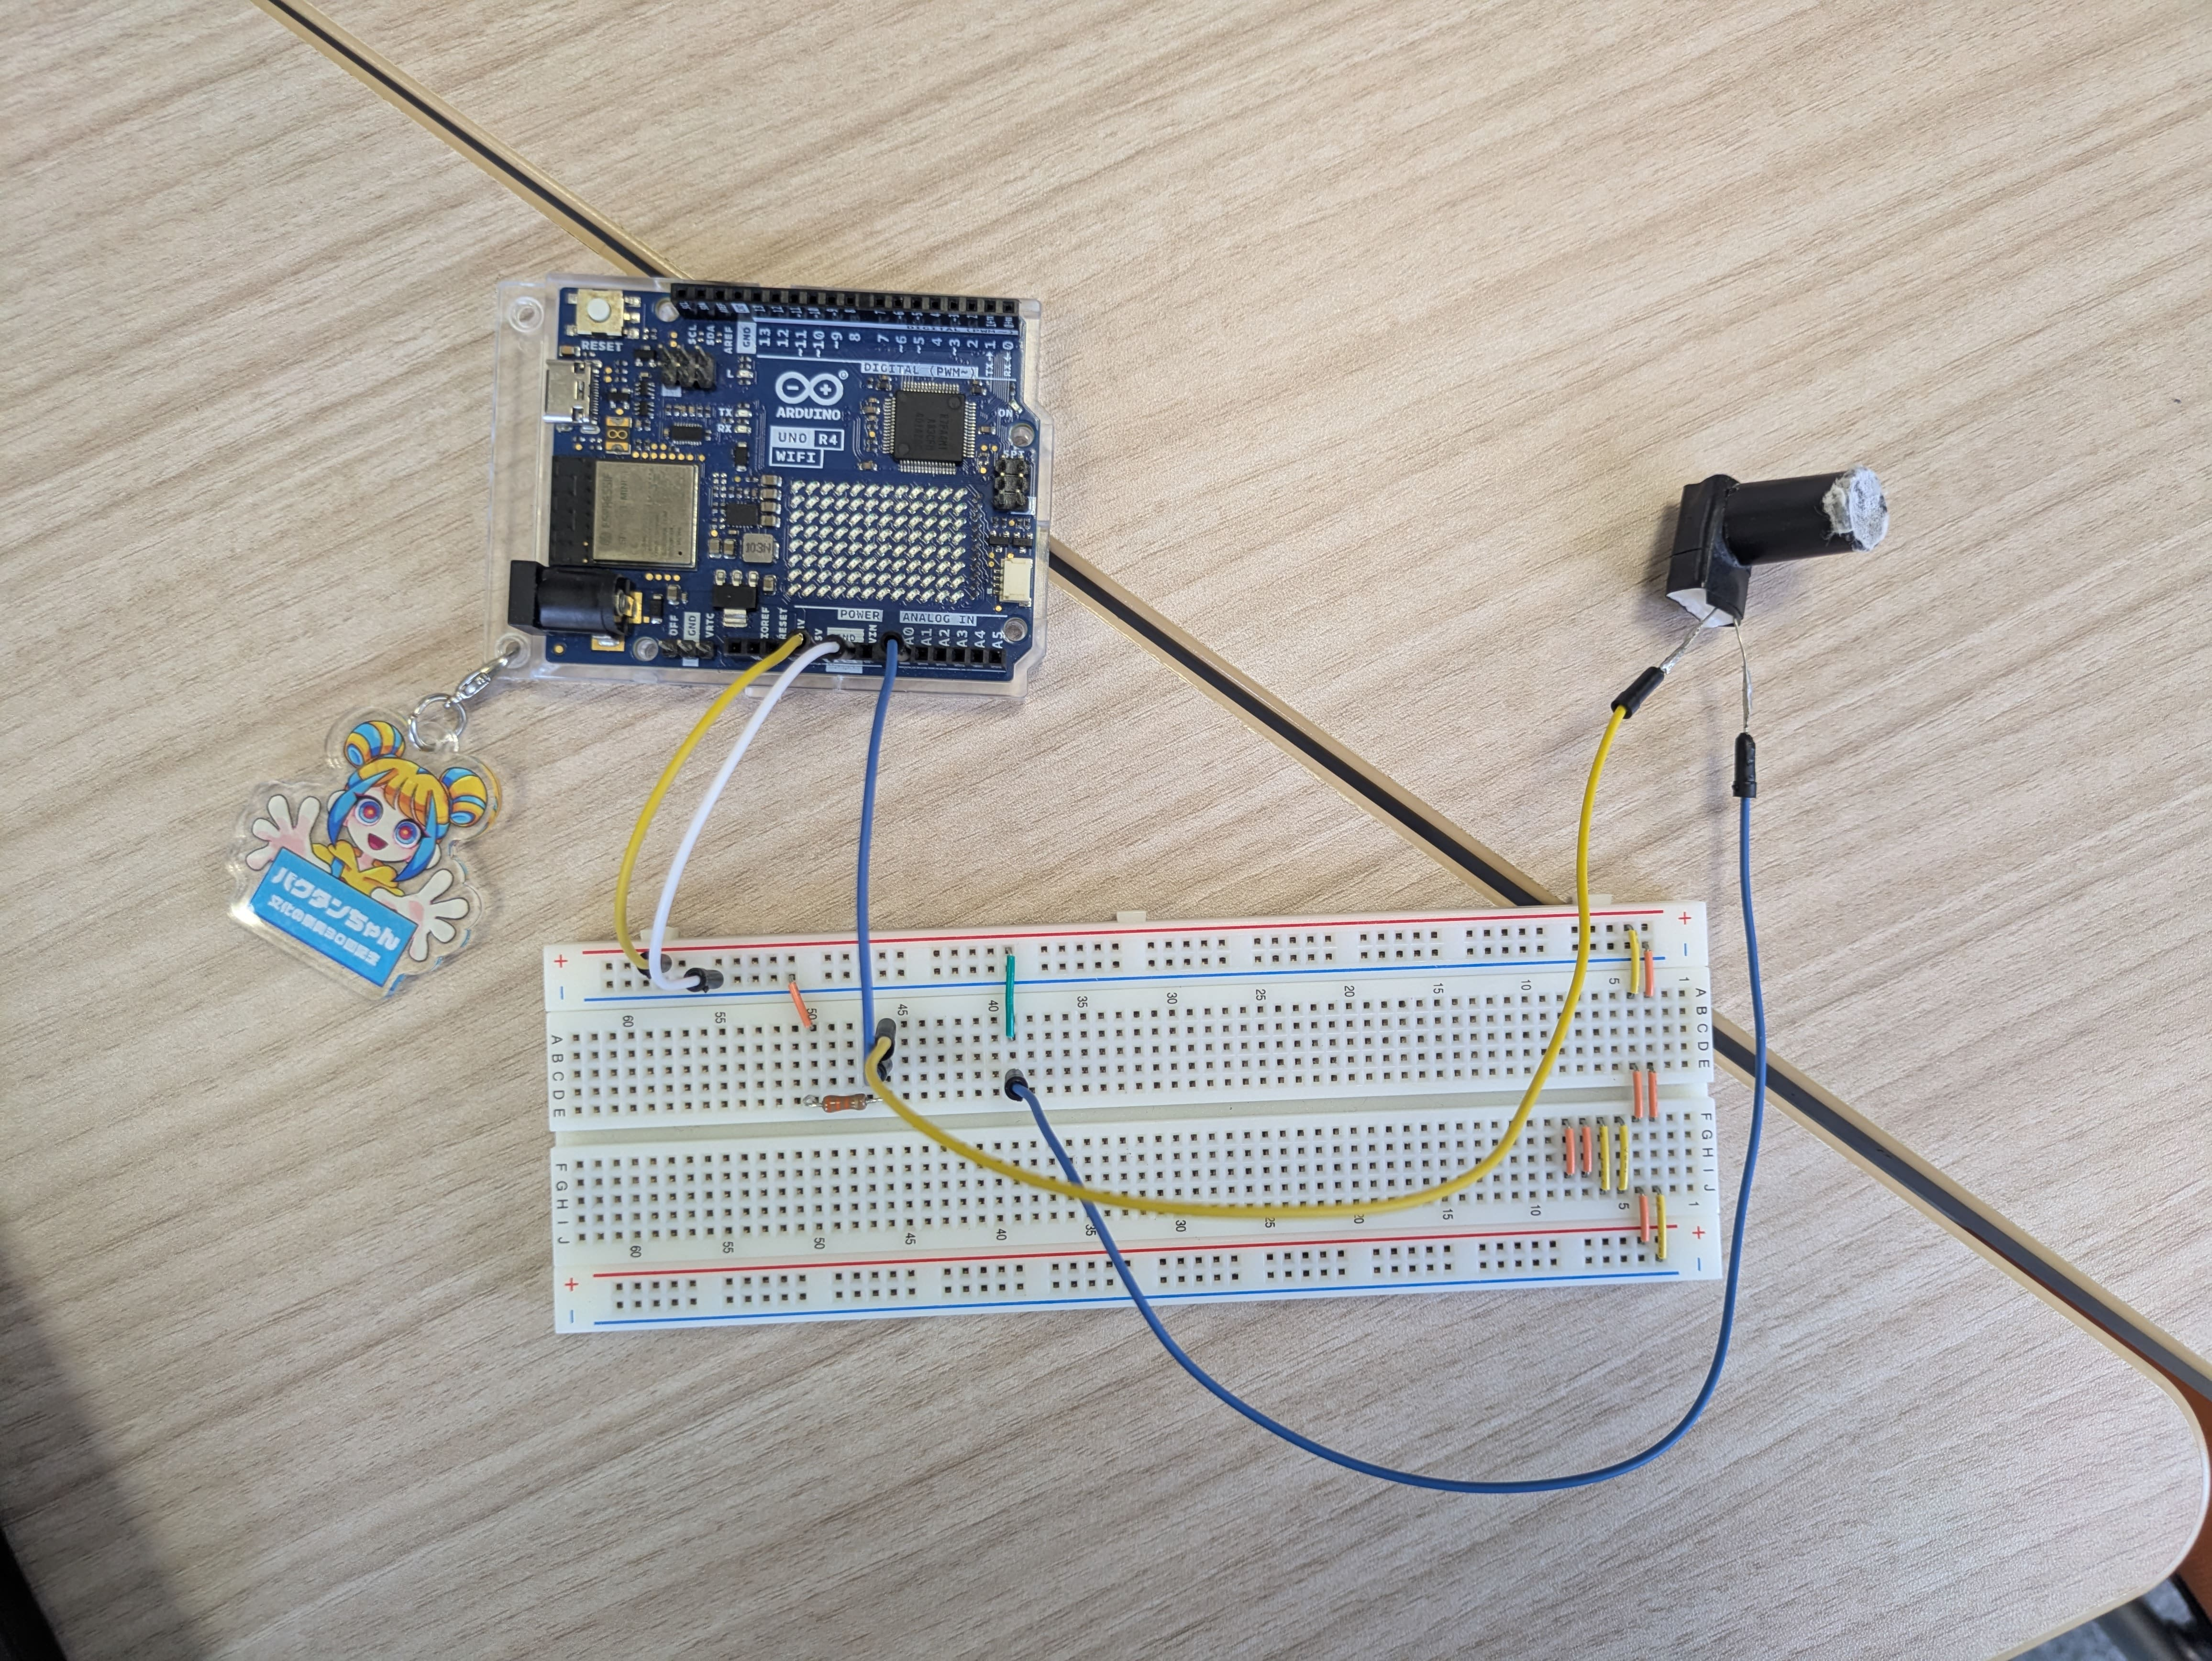
\includegraphics[width=0.6\textwidth]{figs/R_yomitori.jpg}
  \caption{受光部回路の実装}
  \label{fig:r_yomitori}
\end{figure}

\begin{figure}[htbp]
  \centering
  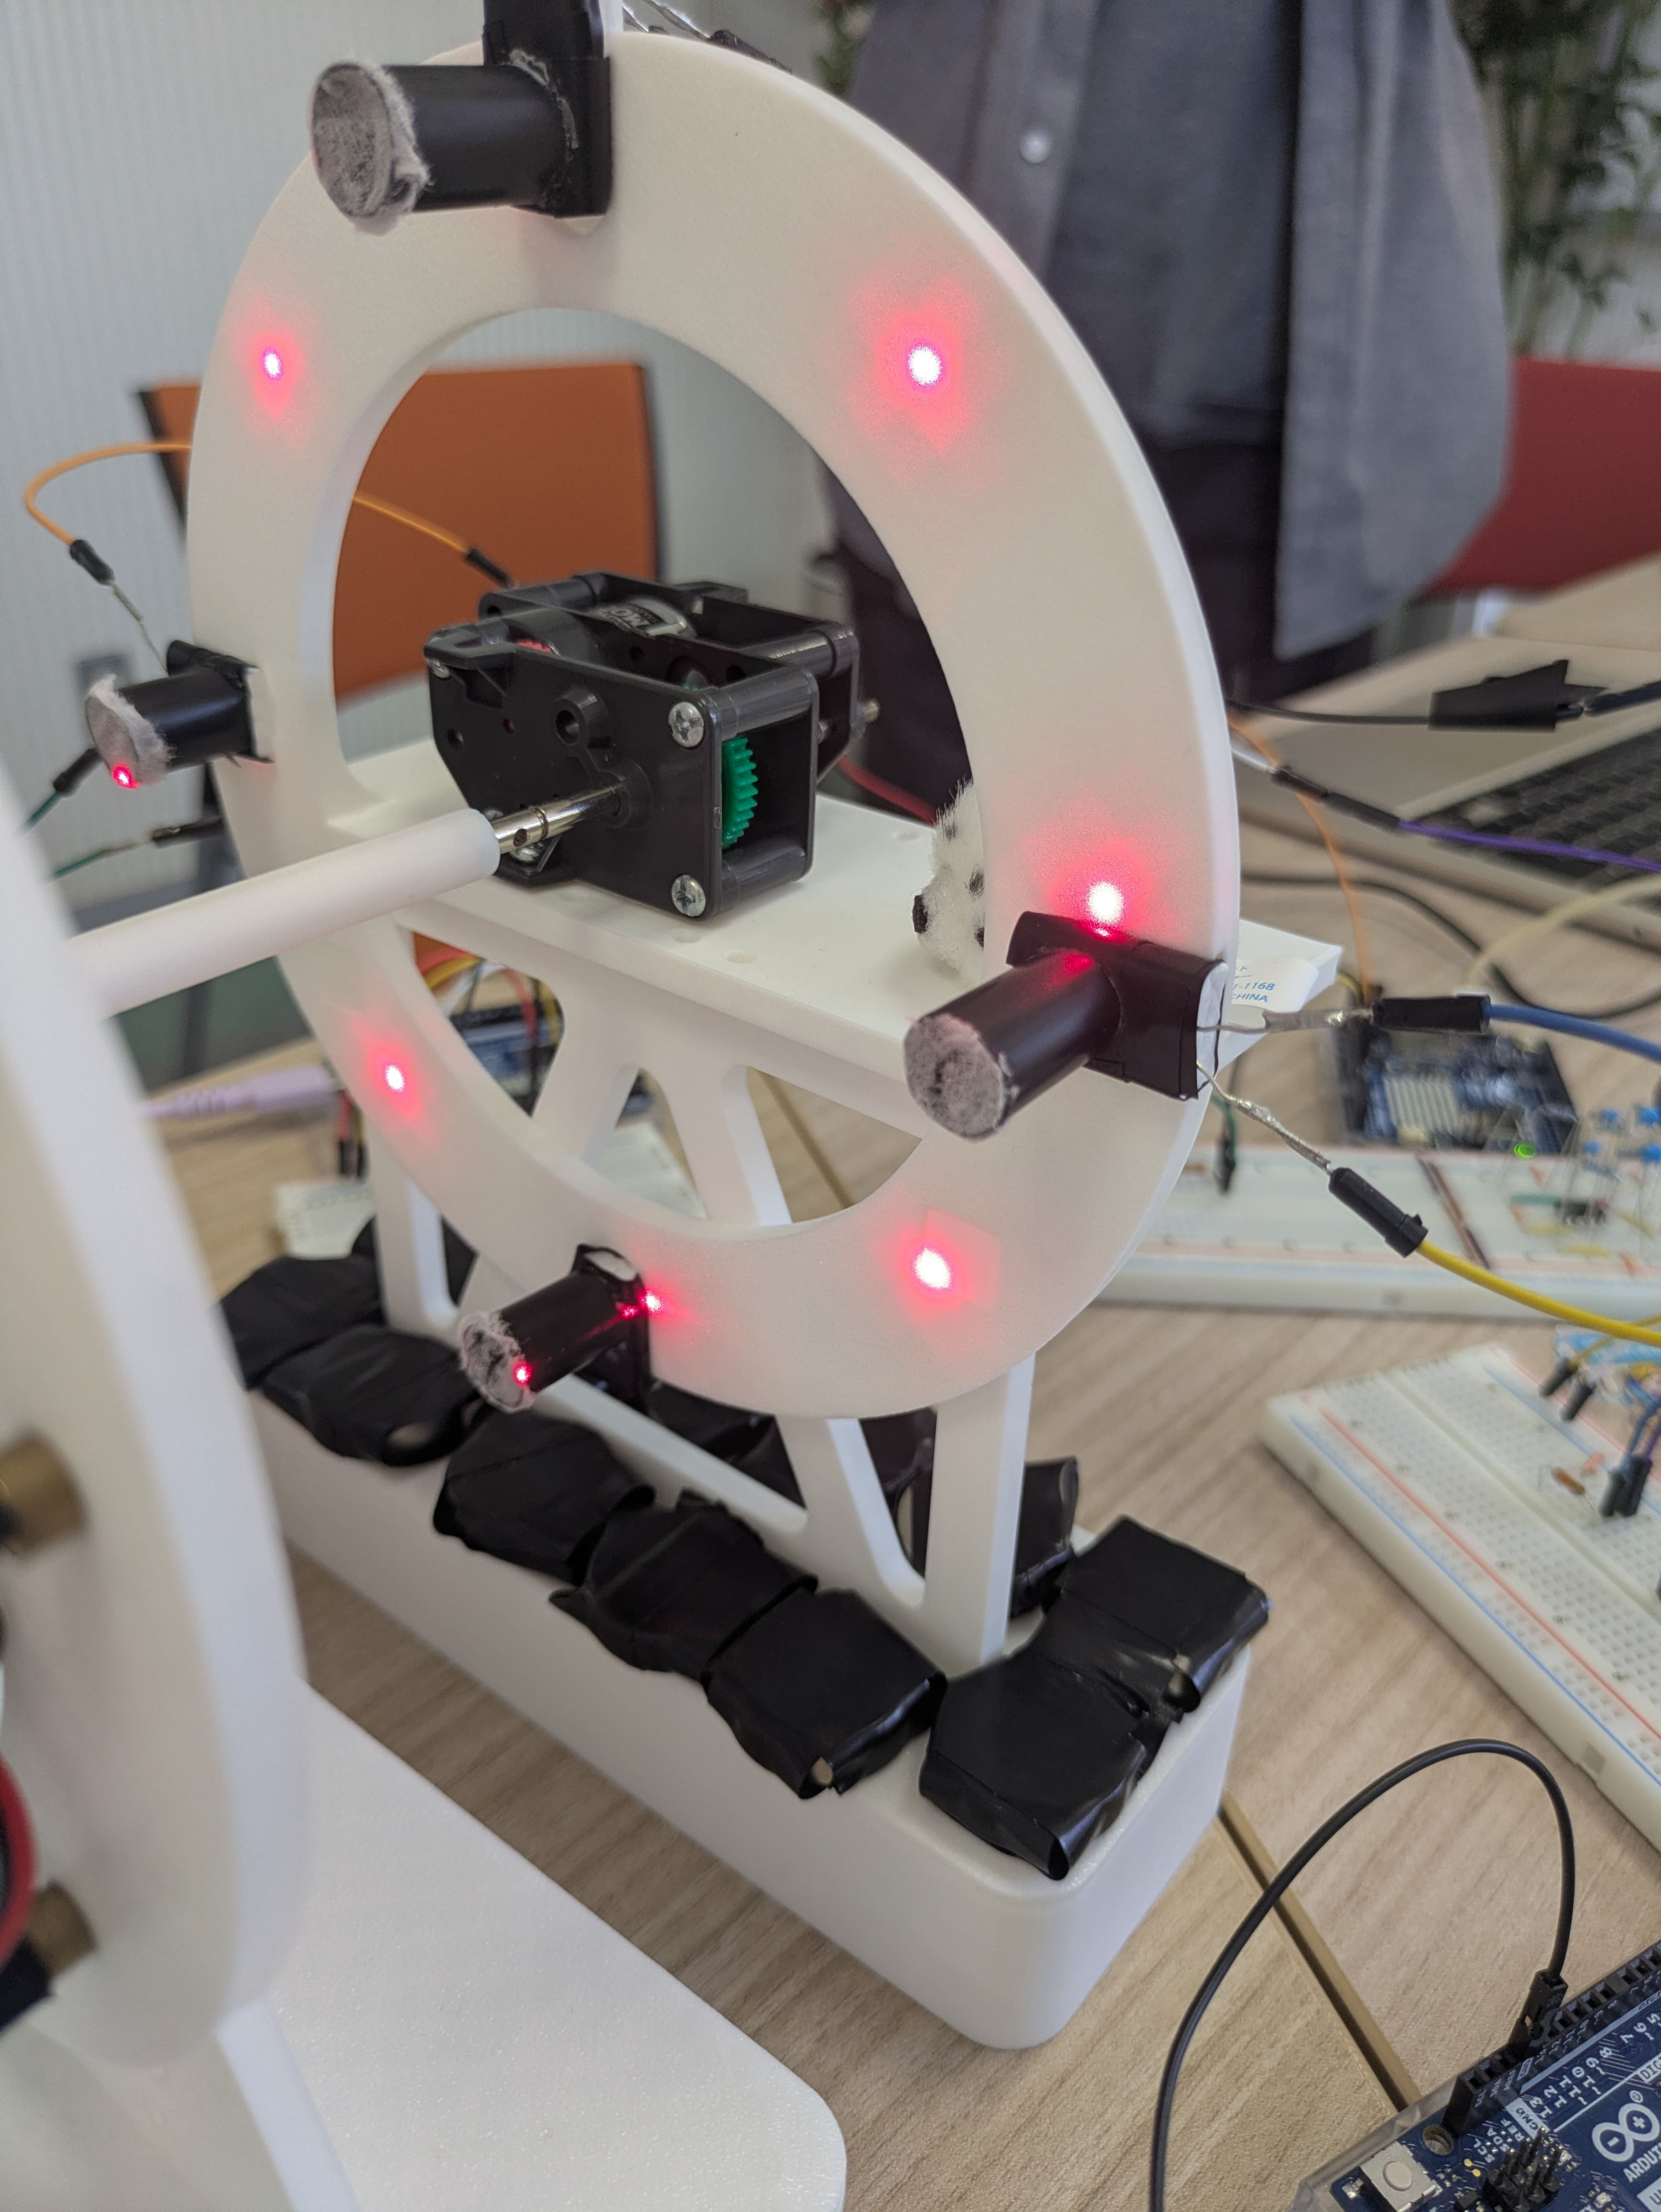
\includegraphics[width=0.7\textwidth]{figs/R_jukou.jpg}
  \caption{遮光板リングと受光部の実装}
  \label{fig:r_jukou}
\end{figure}

\FloatBarrier

\subsubsection{LEDMatrix表示プログラム}
\label{sec:jissou_display}

本節では，ソフトウェア面で担当した中継機デバイスのLEDMatrixに現在のBPMを表示するDisplayモジュール（Display.h，Display.cpp）の実装について，採用した技術の選定理由，実装の過程で直面した技術的課題，およびその解決のために行った技術的貢献を説明する．

はじめに，採用した技術とその選定理由について述べる．
第一に，数字の表示には\ref{sec:kan_naibu}項で述べた独自定義の3×5ドットフォントを採用した．これは，8行12列という限られた表示領域に最大3桁のBPM値を収めたうえで，桁間に1列の間隔を確保して可読性を保つためであり，汎用フォントライブラリを用いる方式では文字幅が大きく3桁を表示できないためである．
第二に，フレームバッファの描画方式には，設計当初に予定していた8行12列の2次元配列を直接渡す方式ではなく，96ビット分の表示内容を3個の32ビット整数へビットパックして転送する方式を採用した．これは，後者の方が描画APIへ渡すデータ量が小さくメモリ効率が高いためである．
第三に，受信データの読み込みには，設計当初に予定していた文字列としての読み込みではなく，2バイトのバイナリ形式のまま読み取り，1バイト目をヘッダ文字，2バイト目を段階番号として処理する方式を採用した．これは，\ref{sec:siki_naibu}項で述べた通信プロトコル自体が固定長2バイトのバイナリ形式で定義されており，プロトコル仕様に忠実な実装とするためである．

次に，実装の過程で直面した技術的課題とその解決について述べる．
最大の課題は，コンパイルおよび書き込みは正常に完了するにもかかわらず，LEDMatrixに何も表示されないという不具合であった．この問題の切り分けのため，起動時の点灯テストや診断用の描画処理を一時的に追加し，どの段階で表示が失われるかを段階的に確認した．その結果，原因は使用したLEDMatrix制御ライブラリの内部構造にあることが判明した．本ライブラリの表示バッファはヘッダファイル内でstatic変数として定義されているため，ヘッダを取り込んだソースファイルごとに別々の実体が生成される．このため，メインスケッチ側で初期化を行い，Displayモジュール側で描画を行う構成では，初期化と描画が互いに異なる実体に対して行われ，表示が反映されなかった．この解決として，初期化と描画を含むマトリクスへの全操作をDisplay.cpp内へ集約し，初期化用の関数（displaySetup）を新設してメインスケッチからはこれを呼び出す構成へ変更した．さらに，初期化直後の最初の描画が反映されない場合がある事象に対しては，初期化時に消灯フレームを一度描画してから\SI{200}{ms}待機するウォームアップ処理を設けることで，以降の描画を確実に反映させた．この一連の対応により，ライブラリ内部の実装に依存する不具合を，モジュール構成の見直しによって解決した．

また，設計段階の関数構成に対して，実装段階で次の機能追加を行った．演奏終了の指令（ヘッダ'E'）を受信した際にLEDMatrixを全消灯する処理は，通信プロトコル上はヘッダが定義されていたものの，設計段階の表示側関数一覧には対応する処理の記載がなかったため，消灯用の関数（clearDisplay）を追加して対応した．あわせて，桁単位の描画を行う内部関数（drawDigit）を分離することで，表示処理の見通しを改善した．

開発の経過は次の通りである．まず表示機能の骨格を作成し，設計書に沿ってBPM表示機能を実装した．この際，通信部を一時的に無効化し，与えたBPM値の描画のみを単体で検証できる状態とした．その後，前述の無表示問題の切り分けと修正を行い，表示の安定化を確認した．続いて，演奏終了時の消灯処理を追加するとともに通信部を有効化し，最後に，指揮デバイスの送信先アドレスと一致させるための静的IPアドレス設定を追加して，結合テストへ移行した．なお，開発段階では表示モジュール単体での検証のために受信処理を仮実装していたが，結合にあたっては，UDP受信を中継機デバイス本体のプログラム側で行い，Displayモジュールは描画専用とする構成に整理した．

\FloatBarrier

\subsection{開発支援ツール（生成AIを含む）の活用と検証}
\label{sec:jissou_ai}

本節では，開発過程で利用した支援ツールおよび情報源と，その利用目的・検証方法について述べる．
まず，技術情報源として，Arduino公式リファレンス，および使用した各部品のデータシートを参照した．部品の定格・接続仕様はデータシートの記載に基づいて決定し，回路実装前に確認した．
次に，生成AI（Anthropic社のClaude）を，次の3つの目的で利用した．第一に，\ref{sec:jissou_display}節で述べたLEDMatrix表示プログラムの実装補助である．第二に，評価データの統計処理およびグラフ生成用Pythonスクリプトの作成である．第三に，本稿のLaTeX原稿の草稿作成・推敲およびレイアウト調整の補助である．
LEDMatrix表示プログラムの実装では，生成AIを次の場面で利用した．実装の初期段階では，LEDMatrix制御ライブラリの利用方法や関数の仕様について質問し，実装の方針検討に用いた．ただし，回答に含まれるライブラリ名や関数名が実際の開発環境に存在しないものである場合があったため，回答をそのまま採用せず，Arduino公式リファレンスと照合して実在する名称・仕様へ修正したうえで，妥当と判断した部分のみを採用した．次に，前述のLEDMatrixに何も表示されない不具合の調査では，症状と構成を提示して原因の候補と切り分け手順の提案を受け，提案された診断手順を実機で順に実行することで，表示バッファの実体がソースファイルごとに分かれるという原因の特定に至った．このとき提案された「マトリクスへの操作を一つのソースファイルへ集約する」という修正方針は，原因の説明として整合することをコード上で確認したうえで採用した．
また，演奏終了指令の受信時に全消灯を行う処理の実装方針についても提案を受け，コンパイルと実機での表示確認により動作を検証したうえで採用した．
生成AIの出力は，次の方法で検証したうえで採否を判断した．
プログラムに関する出力については，コンパイルの成否，実機での動作，およびシリアルモニタでの出力値の確認により妥当性を検証し，さらにライブラリや関数の仕様に関する記述はArduino公式リファレンスと照合して，意図と異なる動作をする生成結果や事実と異なる記述は修正または破棄した．統計処理については，算出された統計量を教員から配布された集計シートの値と照合し，一致することを確認した．また，グラフおよび表の数値は生データからの再計算によって確認した．LaTeX原稿については，コンパイル結果の出力および図表の配置を確認するとともに，記載内容が実際の実装・測定結果と一致しているかを照合し，事実と異なる記述や根拠のない表現は修正または削除した．いずれの利用においても，生成結果をそのまま採用するのではなく，内容を理解したうえで最終的な採否と修正を判断した．

\FloatBarrier

\section{評価方法と結果}
\label{sec:hyouka}

% 本節では，作成したシステムの有効性を評価するために実施した単体テストと結合テストの評価指標と結果について説明する．
% 本システムは，空間全体への多感覚的なフィードバックを通じて，利用者の没入感および関与感を高めることを目的としていた．

\subsection{単体テスト}
\subsubsection{評価方法}
\label{sec:tanka_method}

単体テストでは，各デバイスを結合する前の段階で，デバイス単位・機能単位での基礎的な処理精度を個別に評価する．

はじめに，指揮デバイスの単体テストについて説明する．
指揮デバイスは，ボタン判定の制御テストと加速度センサの制御テスト，そしてBPM・音量の読み取りテストを実施する．ボタン判定の制御テストとは，タクトスイッチを押下してから中継機デバイスが動作するか確認するテストであり，複数回ボタンを押下し，中継機デバイスが回転を開始する成功率を測定することで評価する．また，タクトスイッチを押下してから中継機デバイスが反応し動作するまでの時間を計測することで，ボタン入力から動作開始までの応答遅延が許容範囲内であるか評価する．この時，Nielsenはユーザインタフェースにおける応答時間の閾値として，0.1秒（即時応答の知覚限界），1.0秒（思考の流れを維持できる限界），10秒（タスクへの注意を保持できる限界）の3段階を提示している\cite{nielsen1993}．Nielsenによると10秒を超える遅延に対しては，ユーザはタスクから注意を逸らし，別の作業を行おうとする傾向があるとされる．この知見に基づき，ボタン押下から中継機デバイスの動作開始までの応答遅延が10秒以内である場合を許容範囲内と定義する．
加えて，指揮デバイスのボタンを押下してから実際に楽器デバイスのPCから楽曲が再生されるまでの応答遅延時間も計測し，許容範囲内であるか評価する．Tanらは，HCIおよび認知心理学における確立された遅延閾値として，60秒に達するとユーザは注意を完全に離脱させるか，システムの故障やコンテンツ品質の低さといった否定的な解釈を行う傾向があることを示している\cite{tan2026}．この知見に基づき，ボタン押下から楽曲再生開始までの応答遅延が60秒を超過した場合は異常として打ち切り，60秒以内である場合を許容範囲内と定義する．
さらに，連打や長押しをした場合，意図しない動作をしないか確認する．

次に加速度センサの制御テストとは，指揮デバイスにおける振り動作の判定に関するテストである．\ref{sec:siki_naibu}項で述べた通り，加速度センサの制御処理は差分算出，多重検知防止，状態の反転という段階的な検知ロジックを実装している．そこで，検知閾値が正しく設定されているかを確認する．この閾値が正しく設定されていないと，一度の振る動作で複数回検知されたり，振っても検知されないことが起きる．評価方法はシリアルモニタを用いて実測加速度値と判定結果（演奏状態フラグの反転タイミング）を出力し，意図した振り動作に対して正しく検知できているか，また多重検知や停止状態での誤反応が生じていないかを確認する．また，指揮デバイスを振ったと判断されるまでの遅延を計測し，体感として許容範囲であるか評価する．ここで計測する時間とは，指揮デバイスを振ってから中継機デバイスの動作に反映されるまでの応答遅延時間である．この許容範囲についても，ボタン判定の制御テストと同様にNielsenの示す応答時間の閾値\cite{nielsen1993}に基づき，中継機デバイスの動作開始までの応答遅延が\SI{10}{s}以内である場合を許容範囲内と定義する．


最後に，可変抵抗器によるBPM・音量読み取りテストとは，指揮デバイスの可変抵抗器を操作し，変更された情報が正確に中継機デバイスへ伝達・反映されるかを確認するテストである．\ref{sec:pot_detail}項で述べた通り，BPM・音量読み取り機能は，移動平均処理により可変抵抗器のアナログ値を平滑化したうえで，5段階のBPM・音量の段階番号へ変換する処理を行っている．本テストでは，指揮デバイスを操作して振ってから，中継機デバイスの回転速度が変化するまでの時間を計測するとともに，変更した段階が正しく反映されているかの確認および成功率の計測を行った．


次に，中継機デバイスの単体テストについて説明する．
中継機デバイスは，デバイスの回転制御テストを実施する．これは，最遅BPMであるBPM60の場合と，最早BPMであるBPM180の場合において，モータが止まらずに稼働するかを確認する．加えて，中継機デバイスの物理負荷テストとして，BPM180の場合においても長時間稼働し続けられるか確認する．この時，長時間とは中継機デバイスが回転を開始してから同期をし，一曲演奏し終わるまでの時間と定義する．また，中継機デバイスのArduinoに搭載されているLEDMatrixの表示が現在のBPMを反映しているか確認する．



最後に，楽器デバイスの単体テストについて説明する．
楽器デバイスは，レーザー光受光の検知テストと各楽器の音色再現度テストを実施する．
楽器デバイスの受光部は，CdSセルの暗状態における出力の推定値を継続的に追従させながら，検知閾値を実測値に基づいて動的に更新する適応閾値方式を採用している（\ref{sec:gakki_naibu}項）．レーザー光受光検知テストでは，レーザー光の点灯・消灯を手動で切り替え，検知パルスの立ち上がり・立ち下がりのタイミングをシリアルモニタで確認することで，安定して受光を検知できているかを評価する．

また，各楽器の音色再現度のテストとは，作成した音源(ストリングス，フルート，ピアノ，ハイハット，キックドラム，スネアドラム)と実際の楽器音との類似度をアンケート調査によって評価するテストである．アンケート方式は，計画書当初は各楽器について3種類の音色パターンを提示し比較する方式を検討していたが，回答者1人あたりの回答時間が長くなり十分なサンプル数を確保することが難しいという問題があったため，実際は提示する参考音（実楽器音）と自作音を1対1で比較する方式に変更し，回答1件あたりの所要時間を短縮した．被験者100名に対し，実際の楽器音（参考音）と自作音を1対1で提示し，両者の類似度を1〜5の5段階リッカート尺度（1: 全く似ていない，2: あまり似ていない，3: どちらともいえない，4: ある程度似ている，5: 非常に似ている）で回答を得た．

本テストの評価指標には，MOS（Mean Opinion Score）評価を採用する．MOS評価とは，ITU-T勧告P.800\cite{itu_p800}で標準化された主観品質評価手法であり，被験者が音の品質を5段階の絶対範疇尺度（1: Bad〜5: Excellent）で評定し，その代表値によって品質を判定するものである．MOS評価は音声・音響分野における主観品質の標準的な評価手法として広く用いられており，本テストのように「合成音が実楽器音にどれだけ近いか」という聴感上の品質を被験者の評定によって定量化する目的に整合する．MOS評価において評定値4は「Good（良い）」に相当し，実用上十分な品質と判断される水準である\cite{itu_p800}．

MOPとは，性能指標の略であり，システムが要求される性能をどの程度満たしているか定量的に評価するための指標である．本プロジェクトでは，まずシステムの成果物が目的に対してどのような効果を発揮すべきかを示す上位の定性的な指標として，MOE(Measure of Effectiveness：効果指標)を定義している．音色再現に関するMOEは，「音色の再現ができているか」であり，MOPはこのMOEを客観的に判定するために設定した具体的な数値基準である．本テストでは，MOS評価にならい，MOPの目標値を「回答分布の中央値および最頻値がともに4.0以上」とする．なお，リッカート尺度は順序尺度であり，評定値間の間隔が等しいことは保証されないため，回答分布の代表値としては平均値ではなく中央値と最頻値を用いる．また，回答分布の散らばりを評価するため，補間を行わない経験分布関数に基づく四分位数（第1四分位数$Q_1$，第3四分位数$Q_3$）および四分位範囲（IQR）を併せて算出する．

% --- 以下，CSATスコアによる評価方法（旧版）はMOS評価への変更に伴いコメントアウト ---
% MOPとは，性能指標の略であり，システムが要求される性能をどの程度満たしているか定量的に評価するための指標である．本プロジェクトでは，まずシステムの成果物が目的に対してどのような効果を発揮すべきかを示す上位の定性的な指標として，MOE(Measure of Effectiveness：効果指標)を定義している．音色再現に関するMOEは，「音色の再現ができているか」であり，MOPはこのMOEを客観的に判定するために設定した具体的な数値基準である．計画書では，このMOPの目標値を「中央値および最頻値がともに4.0以上」としていたが，\SI{50}{ms}（ハース効果）や\SI{10}{s}・\SI{60}{s}（Nielsen，Tan）のような外部文献に基づく根拠を伴う他のMOPとは異なり，「4.0」という値自体に理論的な根拠は示されていなかった．そのため，本テストのMOPには，\ref{sec:ketsugo_method}項（結合テスト）のエンターテイメント性評価でも用いたCSATスコア（Customer Satisfaction Score）を採用し，一般的な企業のCSATスコアの平均値\cite{acsi}を参考とした75\%以上をMOPの目標値とする．CSATスコアは，回答のうち4（ある程度似ている）または5（非常に似ている）と回答した割合として算出する．
%
% さらに，CSATスコアはアンケートという有限のサンプルから得られた比率の点推定値であり，サンプルサイズに依存した推定の不確実性を伴う．そこで，点推定値のみによる判定（非標準化）に加えて，95\%Wilson信頼区間\cite{wilson1927}の下限値がMOPの目標値を上回っているかによる判定（標準化）を併用し，推定の不確実性を考慮したうえでMOPの達成状況を評価する．なお，リッカート尺度は順序尺度であるため，回答分布の代表値としては平均値ではなく中央値と最頻値を用いる．

単体テストで評価する項目とMOPの目標値を表\ref{table:tanka_mop}に示す．

\begin{table}[H]
    \caption{単体テストで評価する性能指標（MOP）}
    \label{table:tanka_mop}
    \centering
    \begin{tabular}{p{5cm}p{8cm}}
    \hline
    \textbf{テスト項目} & \textbf{評価方法とMOP目標値} \\ \hline\hline
    指揮デバイス：ボタン判定の制御テスト & 中継機デバイスが回転を開始する成功率の測定．応答遅延は，中継機デバイスの動作開始まで\SI{10}{s}以内\cite{nielsen1993}，楽器デバイスの楽曲再生開始まで\SI{60}{s}以内\cite{tan2026}．連打・長押し時の誤動作がないこと\\ \hline
    指揮デバイス：加速度センサの制御テスト & シリアルモニタによる実測加速度値・判定結果（演奏状態フラグの反転タイミング）の確認．多重検知や停止状態での誤反応がないこと．振ってから中継機デバイスの動作に反映されるまでの応答遅延が\SI{10}{s}以内\cite{nielsen1993}であること\\ \hline
    指揮デバイス：BPM・音量読み取りテスト & シリアルモニタによるアナログ値・変換後段階番号の確認．可変抵抗器操作から中継機デバイスの回転速度変化までの時間および段階反映の成功率の測定\\ \hline
    中継機デバイス：回転制御テスト & 最遅BPM（BPM60）および最早BPM（BPM180）のいずれにおいてもモータが停止せず稼働すること\\ \hline
    中継機デバイス：物理負荷テスト & BPM180において，回転開始から同期・1曲演奏終了までの間，稼働を継続できること\\ \hline
    中継機デバイス：LEDMatrix表示テスト & 表示内容が現在のBPMと一致していること\\ \hline
    楽器デバイス：レーザー光受光の検知テスト & レーザー光の点灯・消灯に対するパルス検知タイミングの確認（定性的な動作確認であり数値目標は設定していない）\\ \hline
    楽器デバイス：音色再現度テスト & 被験者アンケート（1〜5の5段階評価）に対するMOS評価\cite{itu_p800}に基づき，回答分布の中央値および最頻値がともに4.0以上であること\\ \hline
    % （旧版）楽器デバイス：音色再現度テスト & 被験者アンケート（1〜5の5段階評価）のCSATスコア（4または5の回答割合）75\%以上\cite{acsi}．点推定（非標準化）および95\%Wilson信頼区間\cite{wilson1927}の下限（標準化）の両方で判定\\ \hline
    \end{tabular}
\end{table}





\subsubsection{結果}
\label{sec:tanka_result}

%%%%ぼたん

まず，全160回の試行のうち，中継機デバイスが正常に動作したのは
158回であり，ボタン押下の成功率は98.8\%であった．


ボタン判定の制御テストの結果を表\ref{tab:button_response}に示す．
各BPM設定において複数回のボタン押下を行い，タクトスイッチ押下から中継機デバイスが回転を開始するまでの応答時間を計測した．

応答遅延について，
BPM別の平均応答時間，標準誤差，中央値，最小値，最大値を
表\ref{tab:button_response}に示す．
全BPM設定を通じて，計測された応答時間は
最小$\SI{510}{ms}$，最大$\SI{2030}{ms}$の範囲に収まり，
全試行が約$\SI{2.1}{s}$以内で応答した．
全体の平均応答時間は$\SI{1005.8}{ms}$（標準誤差$\SI{30.0}{ms}$）であった．
これはNielsenが提示する応答時間の閾値$\SI{10}{s}$\cite{nielsen1993}の約10分の1であり，全試行がこの基準を満たした．
 




\begin{table}[htbp]
    \centering
    \caption{BPM別ボタン押下から回転開始までの応答時間}
    \label{tab:button_response}
    \begin{tabular}{crrrrrr}
      \hline
      BPM & 試行回数 & 平均値\,[ms] & 標準誤差\,[ms] & 中央値\,[ms] & 最小値\,[ms] & 最大値\,[ms] \\
      \hline
       60 & 16 & 1231.9 &  81.6 & 1155.0 &  840 & 1950 \\
       90 & 18 &  914.4 &  36.4 &  900.0 &  660 & 1140 \\
      120 & 23 &  884.8 &  37.6 &  890.0 &  510 & 1220 \\
      150 & 14 & 1053.6 & 103.4 &  885.0 &  730 & 2030 \\
      180 & 14 & 1015.7 &  49.1 &  990.0 &  740 & 1410 \\
      \hline
      全体 & 85 & 1005.8 &  30.0 & 950.0 & 510 & 2030 \\
      \hline
    \end{tabular}
  \end{table}

  

  また，連打や長押しを行った場合においても，中継機デバイスが意図しない動作を行う事象は確認されなかった．

次に，指揮デバイスのボタン押下から実際に楽器デバイスのPCで楽曲が再生されるまでの応答遅延について評価する．本測定は，楽器間の同期が確立したと判定するための同期開始条件（許容される同期ズレの閾値）を，\SI{60}{ms}以下とした場合と\SI{50}{ms}以下とした場合の2条件で実施した．測定結果を表\ref{tab:song_start_60ms}および表\ref{tab:song_start_50ms}に示す．

同期開始条件を\SI{60}{ms}以下とした場合，全25回の試行すべてにおいて楽曲再生が正常に開始され，成功率は100\%であった．応答遅延は最小$\SI{4920}{ms}$，最大$\SI{20130}{ms}$の範囲に収まり，全体の平均応答遅延は$\SI{9054.0}{ms}$（標準誤差$\SI{736.5}{ms}$）であった．

\begin{table}[htbp]
    \centering
    \caption{同期開始条件を\SI{60}{ms}以下とした場合のボタン押下から楽曲再生開始までの応答遅延}
    \label{tab:song_start_60ms}
    \begin{tabular}{crrrrr}
      \hline
      BPM & 試行回数 & 平均値\,[ms] & 標準誤差\,[ms] & 中央値\,[ms] & 最小値\,[ms]／最大値\,[ms] \\
      \hline
       60 & 5 &  7816.0 &  355.2 &  7680.0 &  6950 / 8950 \\
       90 & 5 &  6100.0 &  399.9 &  5870.0 &  5070 / 7250 \\
      120 & 5 &  9360.0 &  523.7 &  9700.0 &  7830 / 10910 \\
      150 & 5 &  9768.0 & 1906.5 &  8630.0 &  5000 / 16500 \\
      180 & 5 & 12226.0 & 2616.8 & 12210.0 &  4920 / 20130 \\
      \hline
      全体 & 25 & 9054.0 & 736.5 & 8230.0 & 4920 / 20130 \\
      \hline
    \end{tabular}
\end{table}

一方，同期開始条件を\SI{50}{ms}以下とした場合，全53回の試行（計測ミスにより中断した試行を除く）のうち8回が1分（$\SI{60}{s}$）を超過しても楽曲再生が開始されず，全体の成功率は84.9\%（45/53）にとどまった．特にBPM150では成功率が50.0\%まで低下しており，同期条件を厳格化すると，Tanら\cite{tan2026}の示す\SI{60}{s}という応答遅延のMOP目標値を満たせない試行が生じることが確認された．測定結果を表\ref{tab:song_start_50ms}に示す．

\begin{table}[htbp]
    \centering
    \caption{同期開始条件を\SI{50}{ms}以下とした場合のボタン押下から楽曲再生開始までの応答遅延}
    \label{tab:song_start_50ms}
    \begin{tabular}{crrrrrr}
      \hline
      BPM & 試行回数 & \SI{60}{s}超過 & 成功率 & 平均値\,[ms] & 標準誤差\,[ms] & 最小値\,[ms]／最大値\,[ms] \\
      \hline
       60 &  8 & 2 &  80.0\% & 21065.0 & 5802.5 &  8330 / 50110 \\
       90 &  9 & 1 &  90.0\% & 22417.8 & 5013.0 & 10140 / 58510 \\
      120 & 11 & 0 & 100.0\% & 15430.0 & 2837.3 &  7720 / 38640 \\
      150 &  5 & 5 &  50.0\% & 22872.0 & 7890.2 &  8570 / 52600 \\
      180 & 12 & 0 & 100.0\% & 15339.2 & 2842.5 &  6010 / 31930 \\
      \hline
      全体 & 45 & 8 &  84.9\% & 18632.0 & 1933.4 &  6010 / 58510 \\
      \hline
    \end{tabular}
\end{table}

これらの結果から，本システムでは同期開始条件を\SI{60}{ms}以下に設定することで，指揮デバイスのボタン押下から楽曲再生開始までの応答遅延がMOPの目標値を安定して満たすことが確認された一方，\SI{50}{ms}以下という厳格な条件では，楽器間の同期の確立自体に長時間を要し，MOPを満たせない試行が生じることが明らかになった．

次に，中継機デバイスの単体テストの結果について説明する．回転制御テストでは，最遅BPMであるBPM60および最早BPMであるBPM180のいずれにおいても，モータが停止することなく安定して稼働することが確認された．また，物理負荷テストにおいても，BPM180の条件下で回転開始から同期・1曲演奏終了までの間，中継機デバイスが継続して稼働できることが確認された．さらに，LEDMatrix表示テストでは，表示内容が現在のBPMと一致していることが確認された．以上より，中継機デバイスの単体テストで評価した全項目について，MOPを満たすことが確認された．

続いて，楽器デバイスの単体テストのうち，レーザー光受光の検知テストの結果について説明する．レーザー光の点灯・消灯を手動で切り替え，検知パルスの立ち上がり・立ち下がりのタイミングをシリアルモニタ上で確認したところ，暗状態の出力の推定値に基づく適応閾値方式により，安定して受光を検知できることが確認された．


続いて，各楽器の音色再現度テストの結果について説明する．被験者100名に対する回答の度数分布を表~\ref{tab:response_distribution}に示す．また，回答割合を視覚化した100\%積み上げ棒グラフを図~\ref{fig:stacked_bar}に，各楽器・各評価スコアの回答人数（サンプル数$N$を含む）を示すヒストグラムを図~\ref{fig:score_histogram}に示す．

\begin{table}[htbp]
  \centering
  \caption{各楽器に対する回答の度数分布（$N = 100$）}
  \label{tab:response_distribution}
  \resizebox{\textwidth}{!}{%
  \begin{tabular}{lrrrrr}
    \hline
    楽器 & 1 & 2 & 3 & 4 & 5 \\
         & 全く似ていない & あまり似ていない & どちらともいえない & ある程度似ている & 非常に似ている \\
    \hline
    ストリングス & 0  & 5  & 5  & 42 & 48 \\
    フルート     & 0  & 11 & 5  & 36 & 48 \\
    ピアノ       & 3  & 13 & 13 & 43 & 28 \\
    ハイハット   & 1  & 5  & 5  & 27 & 62 \\
    キックドラム & 3  & 11 & 12 & 49 & 25 \\
    スネアドラム & 1  & 5  & 15 & 49 & 30 \\
    \hline
  \end{tabular}%
  }
\end{table}

\begin{figure}[htbp]
  \centering
  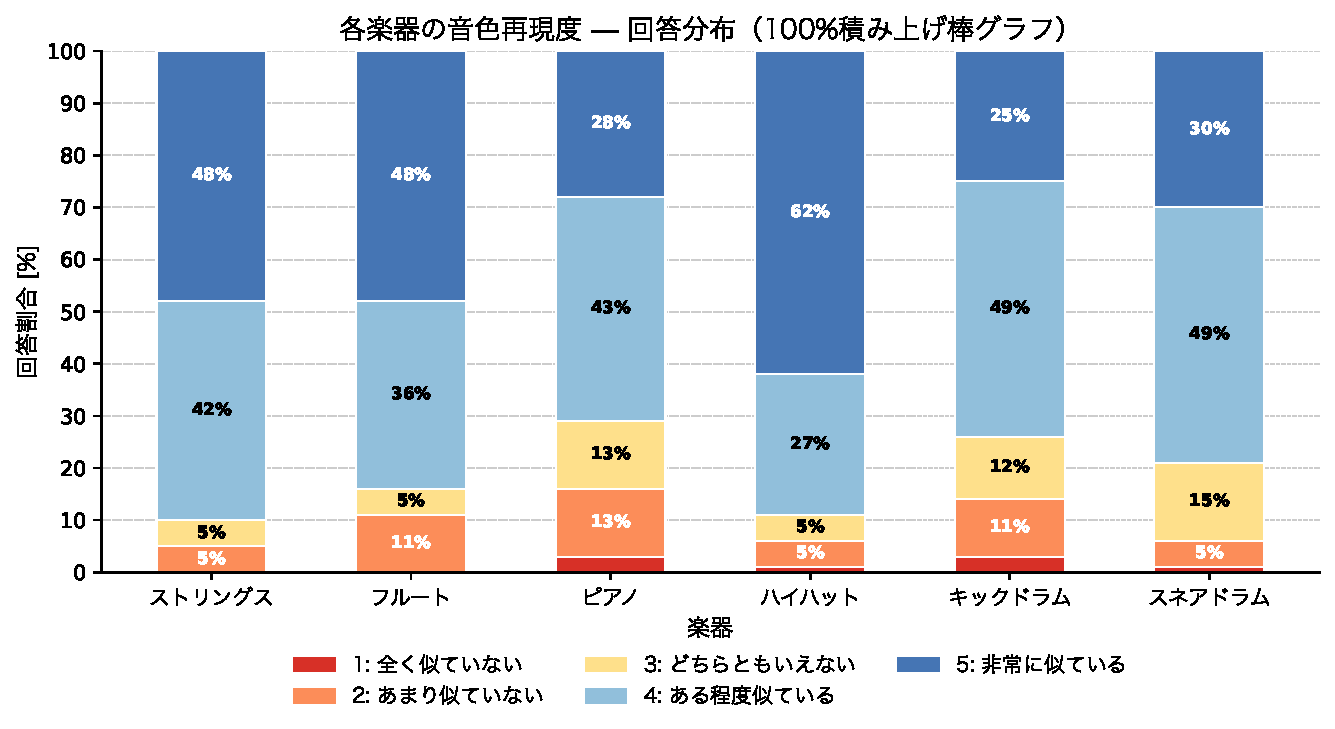
\includegraphics[width=0.92\textwidth]{figs/stacked_bar.pdf}
  \caption{各楽器の音色再現度に対する回答分布（100\%積み上げ棒グラフ）}
  \label{fig:stacked_bar}
\end{figure}

\begin{figure}[htbp]
  \centering
  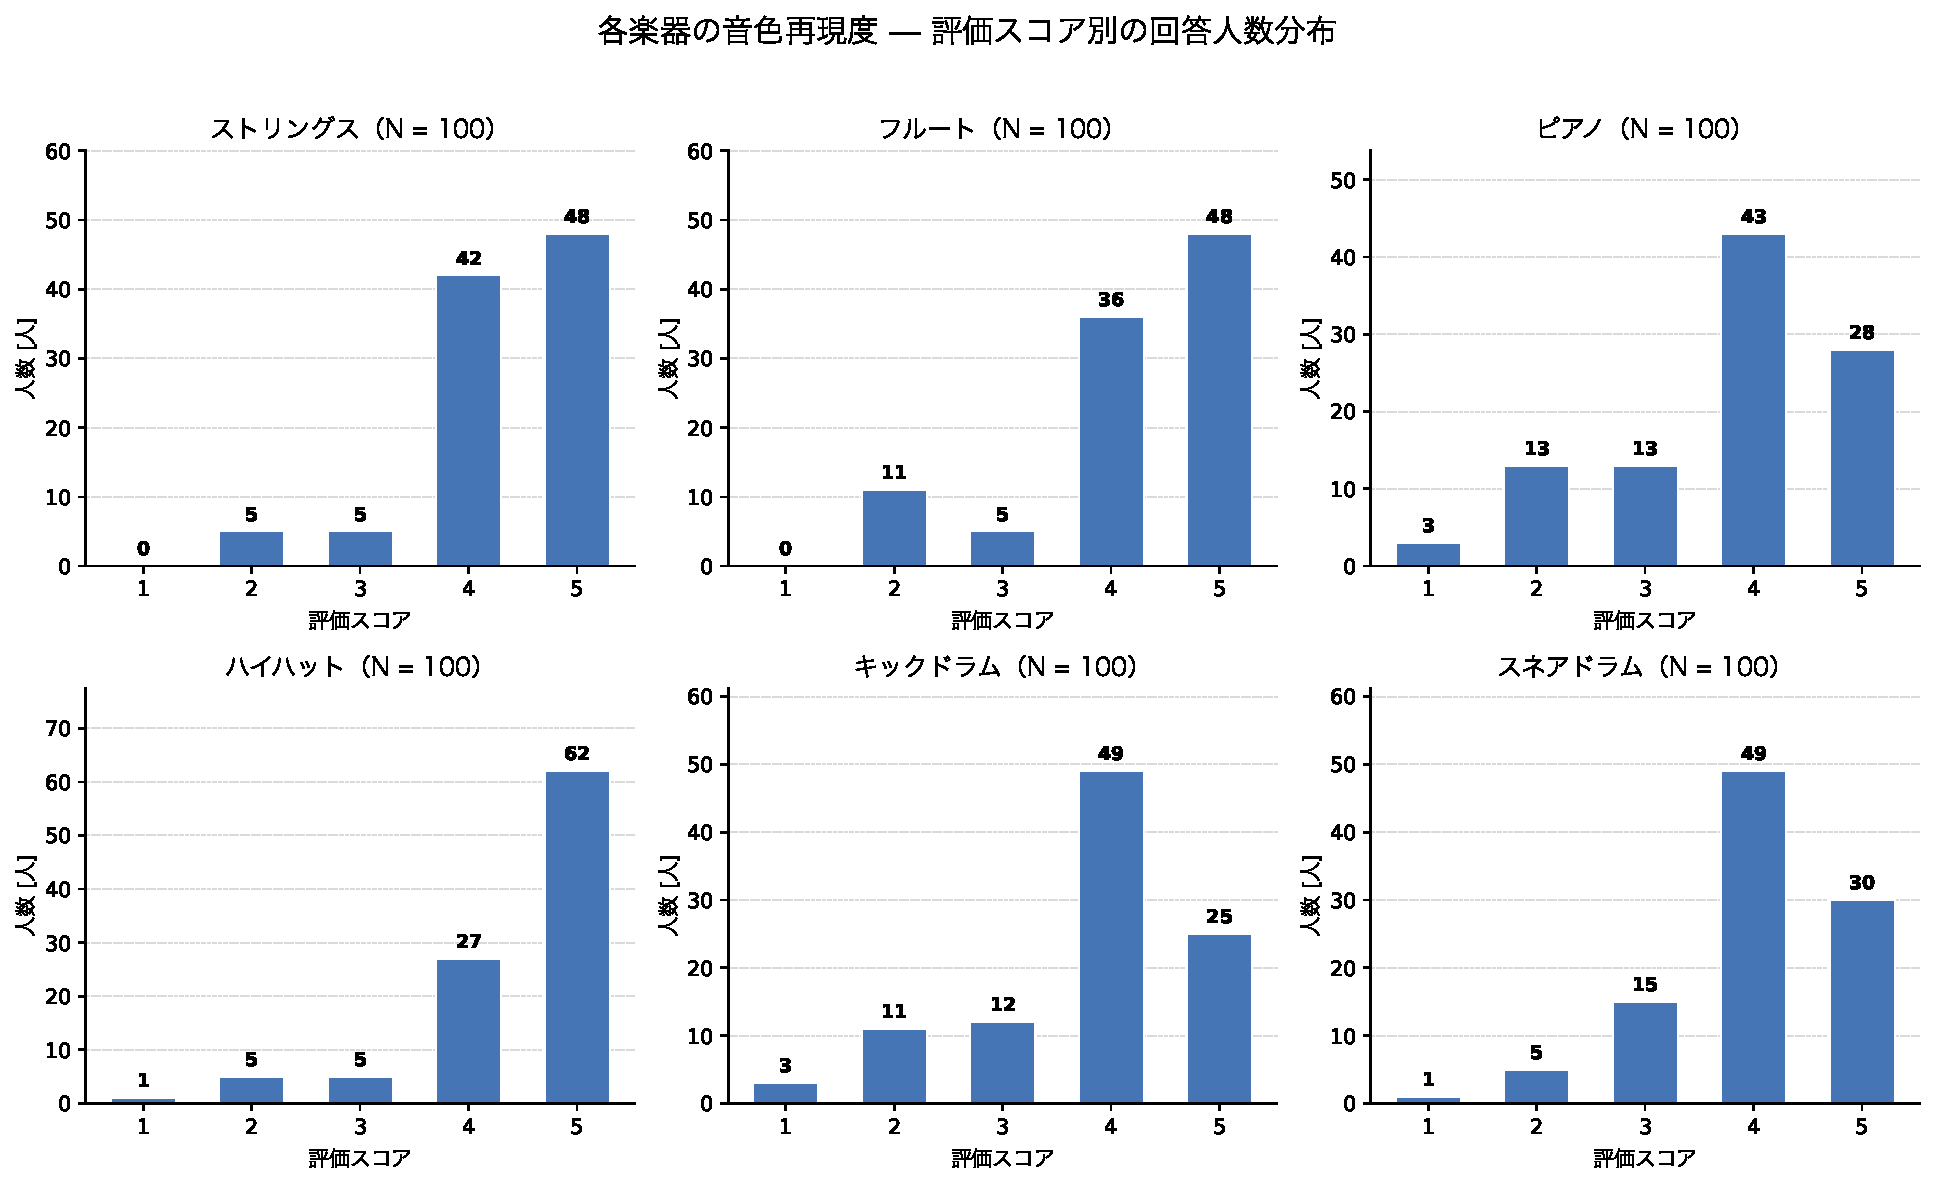
\includegraphics[width=\textwidth]{figs/score_histogram.pdf}
  \caption{各楽器の評価スコア別の回答人数分布}
  \label{fig:score_histogram}
\end{figure}

ハイハットは評価5（非常に似ている）の回答が62\%と最も高い割合を示し，評価4以上の回答が合計89\%を占めた．ストリングスおよびフルートにおいても評価4以上の割合はそれぞれ90\%，84\%であり，高い類似度が認められた．一方，キックドラムでは評価3以下の回答が26\%を占め，6楽器中で最も低い類似度の分布を示した．ピアノについても評価3以下の割合が29\%と比較的高い値を示した．

各楽器の中央値・最頻値および四分位数（$Q_1$，$Q_3$，IQR）と，MOPの目標値（中央値および最頻値がともに4.0以上）に基づく判定結果を表~\ref{tab:median_mode}に示す．また，中央値・最頻値をMOP目標値とともに視覚化した棒グラフを図~\ref{fig:mos_median_mode}に示す．

\begin{table}[htbp]
  \centering
  \caption{各楽器のMOS評価（中央値・最頻値・四分位数）とMOP判定結果（$N = 100$，MOP目標値：中央値・最頻値$\geq 4.0$）}
  \label{tab:median_mode}
  \begin{tabular}{lcccccc}
    \hline
    楽器 & 中央値 & 最頻値 & $Q_1$ & $Q_3$ & IQR & MOP判定 \\
    \hline
    ストリングス & 4 & 5 & 4 & 5 & 1 & 達成 \\
    フルート     & 4 & 5 & 4 & 5 & 1 & 達成 \\
    ピアノ       & 4 & 4 & 3 & 5 & 2 & 達成 \\
    ハイハット   & 5 & 5 & 4 & 5 & 1 & 達成 \\
    キックドラム & 4 & 4 & 3 & 4 & 1 & 達成 \\
    スネアドラム & 4 & 4 & 4 & 5 & 1 & 達成 \\
    \hline
  \end{tabular}
\end{table}

\begin{figure}[htbp]
  \centering
  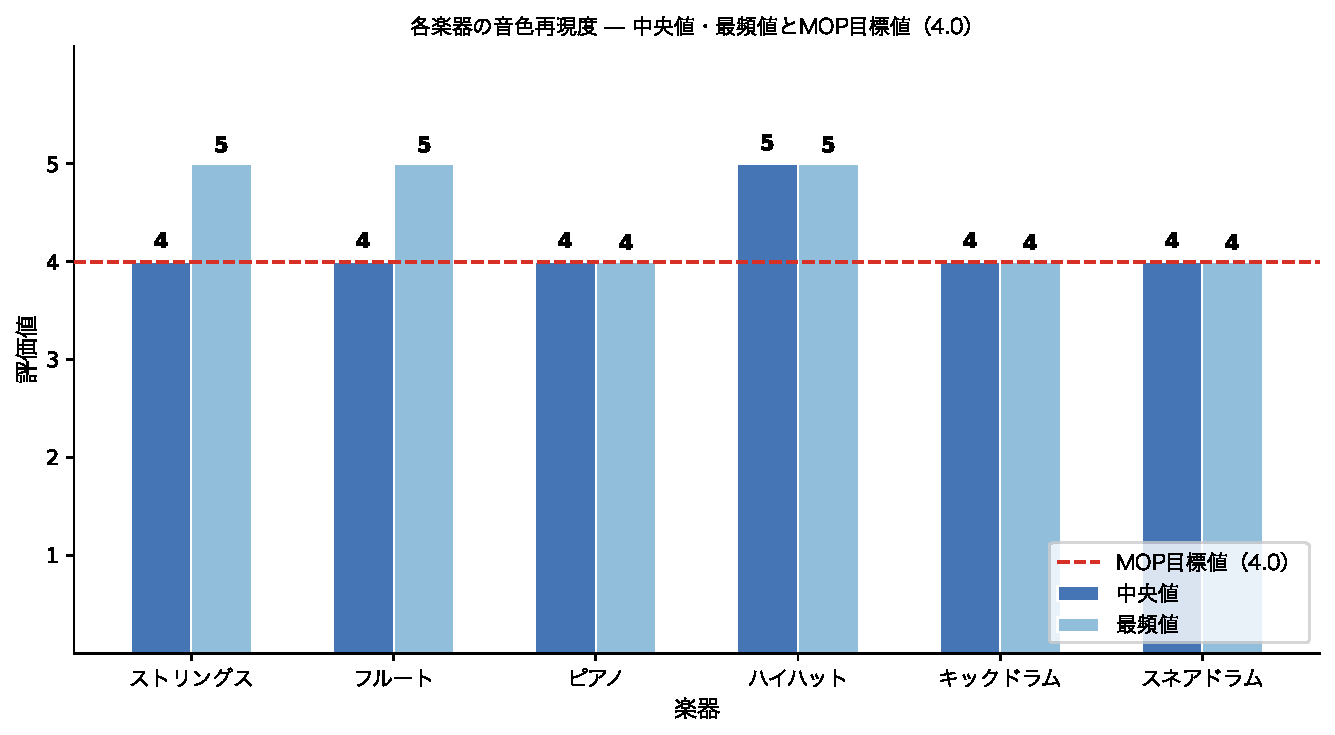
\includegraphics[width=0.92\textwidth]{figs/mos_median_mode.pdf}
  \caption{各楽器の中央値・最頻値とMOP目標値（4.0）の比較}
  \label{fig:mos_median_mode}
\end{figure}

表~\ref{tab:median_mode}に示す通り，全6楽器において中央値および最頻値はともに4.0以上であり，MOS評価に基づくMOPは全楽器で達成された．特にハイハットは中央値・最頻値がともに5であり，6楽器中で最も高い評価を得た．ストリングスおよびフルートは最頻値が5を示し，高い再現性が確認された．一方，回答分布の散らばりに着目すると，ピアノおよびキックドラムは$Q_1$が3であり，回答の4分の1以上が評価3以下に分布している．特にピアノはIQRが2と6楽器中で最も大きく，被験者間で評価が分かれたことを示している．すなわち，MOPの目標値は全楽器で達成されたものの，ピアノおよびキックドラムについては他の4楽器と比較して低評価側への分布の広がりが認められた．

% --- 以下，CSATスコアによる結果（旧版）はMOS評価への変更に伴いコメントアウト ---
% 各楽器のCSATスコア（評価4または5と回答した割合）を，非標準化（点推定のみ）および標準化（95\%Wilson信頼区間\cite{wilson1927}を用いた判定）の両方で算出した．結果を表~\ref{tab:csat_result}に，非標準化の結果を図~\ref{fig:csat_raw}に，標準化の結果を図~\ref{fig:csat_wilson}に示す．
%
% \begin{table}[htbp]
%   \centering
%   \caption{各楽器のCSATスコアとMOP判定結果（$N = 100$，MOP目標値75\%）}
%   \label{tab:csat_result}
%   \resizebox{\textwidth}{!}{%
%   \begin{tabular}{lrrrcc}
%     \hline
%     楽器 & Top2Box人数 & CSATスコア[\%] & 95\%Wilson信頼区間[\%] & MOP判定（非標準化） & MOP判定（標準化） \\
%     \hline
%     ストリングス & 90 & 90.0 & [82.6, 94.5] & 達成   & 達成   \\
%     フルート     & 84 & 84.0 & [75.6, 89.9] & 達成   & 達成   \\
%     ピアノ       & 71 & 71.0 & [61.5, 79.0] & 未達成 & 未達成 \\
%     ハイハット   & 89 & 89.0 & [81.4, 93.7] & 達成   & 達成   \\
%     キックドラム & 74 & 74.0 & [64.6, 81.6] & 未達成 & 未達成 \\
%     スネアドラム & 79 & 79.0 & [70.0, 85.8] & 達成   & 未達成 \\
%     \hline
%   \end{tabular}%
%   }
% \end{table}
%
% \begin{figure}[htbp]
%   \centering
%   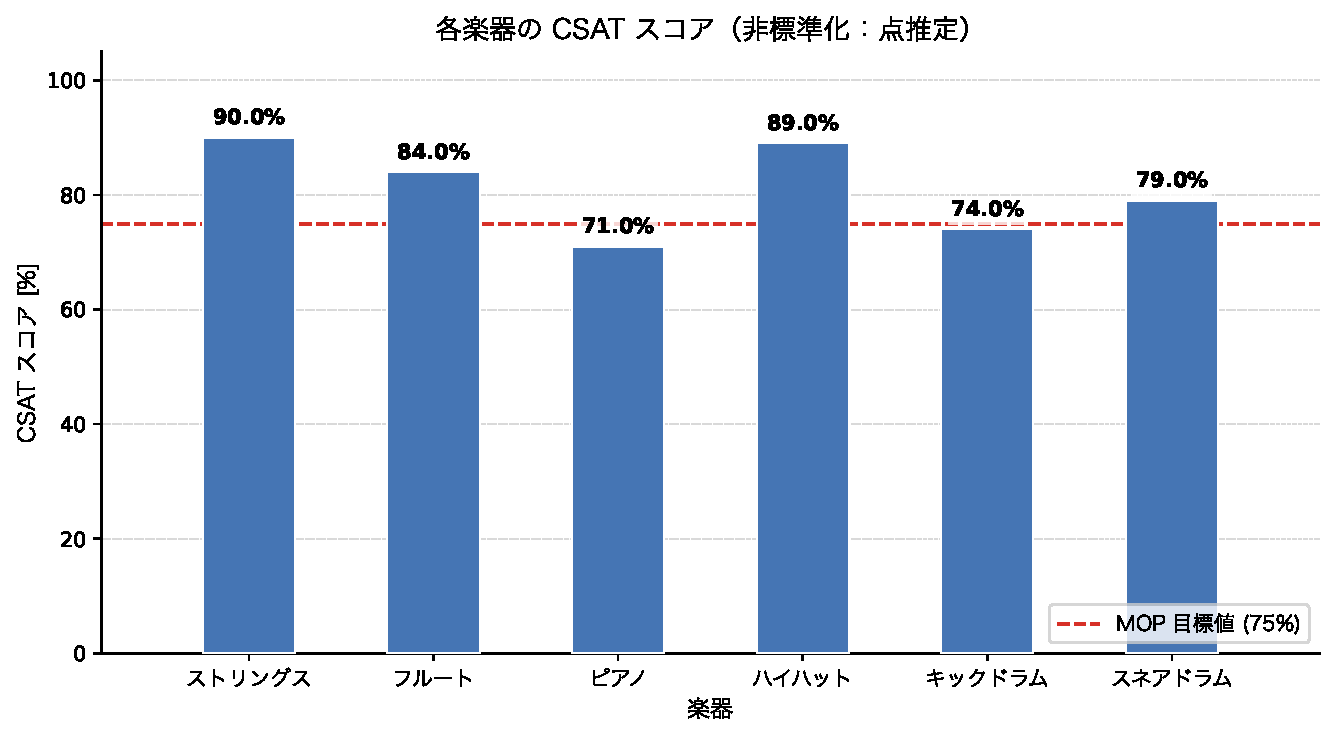
\includegraphics[width=0.92\textwidth]{figs/csat_raw.pdf}
%   \caption{各楽器のCSATスコア（非標準化：点推定）とMOP目標値（75\%）の比較}
%   \label{fig:csat_raw}
% \end{figure}
%
% \begin{figure}[htbp]
%   \centering
%   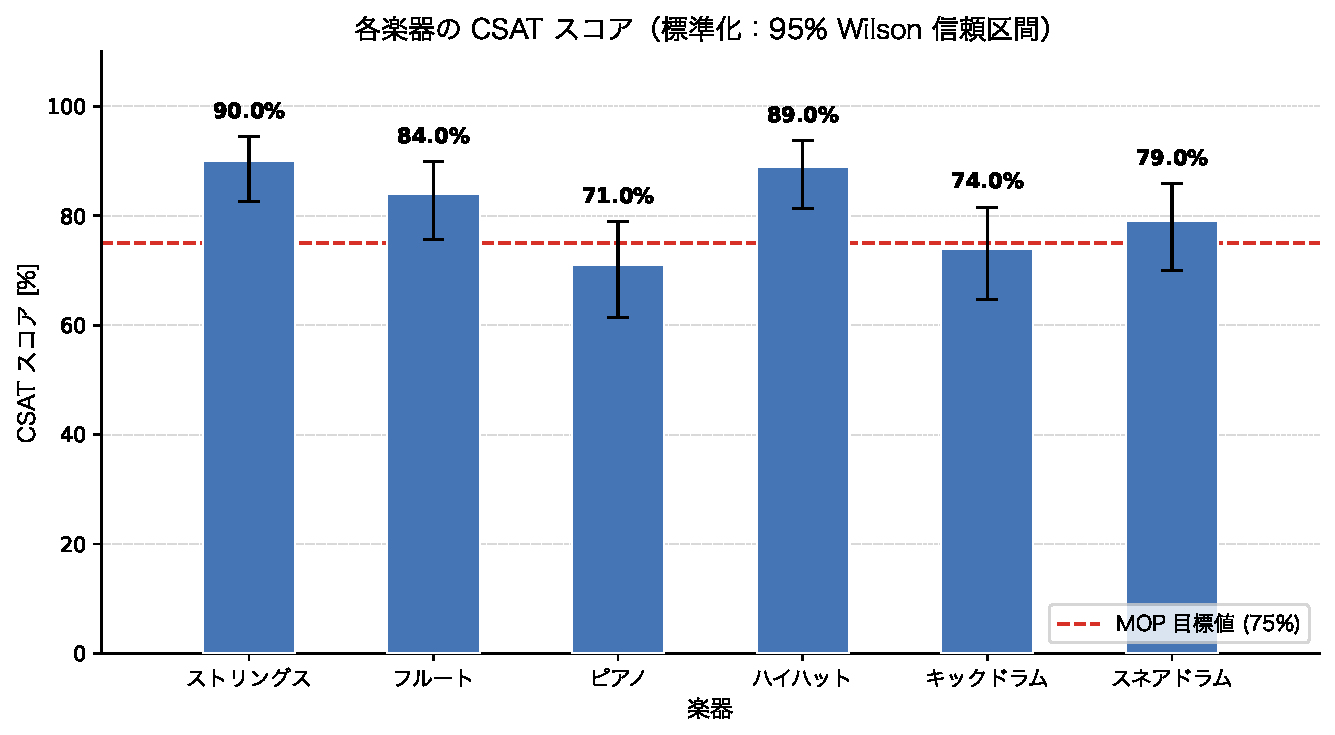
\includegraphics[width=0.92\textwidth]{figs/csat_wilson.pdf}
%   \caption{各楽器のCSATスコア（標準化：95\%Wilson信頼区間）とMOP目標値（75\%）の比較}
%   \label{fig:csat_wilson}
% \end{figure}
%
% 表~\ref{tab:csat_result}に示す通り，非標準化（点推定）で判定した場合，ストリングス，フルート，ハイハット，スネアドラムの4楽器がMOPの目標値である75\%以上を達成した．一方，ピアノおよびキックドラムは，それぞれCSATスコア71.0\%，74.0\%であり，点推定の段階でMOPを達成しなかった．
%
% 標準化（95\%Wilson信頼区間の下限による判定）で判定した場合，達成と判定された楽器はストリングス，フルート，ハイハットの3楽器にとどまった．スネアドラムは点推定では79.0\%とMOPを上回っていたものの，95\%信頼区間の下限が70.0\%であり，サンプルサイズに基づく推定の不確実性を考慮すると，MOPを安定して達成しているとは言い切れない結果となった．ピアノおよびキックドラムは，非標準化・標準化のいずれにおいてもMOPを達成しなかった．
%
% 以上より，非標準化・標準化のいずれにおいてもMOPを達成したのはストリングス，フルート，ハイハットの3楽器であった．ピアノおよびキックドラムは，非標準化・標準化のいずれにおいてもMOPを達成しなかった．スネアドラムは，非標準化では達成と判定されたが，標準化では未達成と判定された．






\FloatBarrier

\subsection{結合テスト}
\subsubsection{評価方法}
\label{sec:ketsugo_method}

結合テストでは，中継機デバイス本体のハードウェア実装と回転制御プログラム，楽器デバイスの受光部と楽曲表現プログラム，および指揮デバイスからのBPM・音量指令を行う通信部を結合した段階で評価を行う．本システムは，指揮デバイスと観覧車型の中継機・楽器デバイスを用いた空間的なフィードバックにより，利用者に高い没入感を与えることを目的として設計されている．そのため，結合テストでは，利用者がこの空間的フィードバックを違和感なく体験できているかという知覚・体験の観点から，「輪唱のタイミングに対して不快に感じる程度の遅延がないか」，「ユーザの操作が正しく反映されるか」，「エンターテイメント性があるか」の3点をMOE（Measure of Effectiveness：効果指標）として定める．これらは，本システムが技術的に動作するだけでなく，利用者の体験として意図した効果を実際に発揮しているかを確認するために設定したものである．

まず，輪唱のタイミングに対して不快に感じる程度の遅延がないかについて評価する．これは，各楽器デバイスの発音タイミングにズレが生じた際，利用者がそれを違和感なく1つの輪唱として聴取できるかを確認するものである．MOPの目標値は，ハース効果\cite{haas1951}（時間差を伴う類似した2つの音を，一定時間内であれば聴覚が1つの音として知覚する現象）の許容限界である\SI{50}{ms}未満とする．なお，\ref{sec:gakki_naibu}項で述べた同期通信（演奏開始時刻を事前に指定して伝える'O'通信の冗長送信等）は，このMOPを満たすことを目的として実装されたものであり，結合テストではこの機構が実際に機能しているかを合わせて確認する．

次に，ユーザの操作が正しく反映されるかについて評価する．評価方法としては，\ref{sec:tanka_method}項（単体テスト）で述べたボタン判定の制御テストおよびBPM・音量読み取りテストと同様に，各デバイスを結合した状態でボタン押下から中継機デバイスの動作反映までの成功率，および指揮棒の操作によるBPM・音量変更が実際に発音へ反映される成功率を計測する．MOPの目標値は，処理成功率99.0\%以上とする．この99\%（ツーナイン）という基準は，一般的なWebサービス等の開発環境において目標とされる稼働率の数値\cite{kobesoft_availability}を参考としたものであり，本プロジェクトで作成するシステムはブレッドボード上で稼働する一つのシステムであるため，テスト環境での運用に近いことから，この数値を目標として採用した．

次に，エンターテイメント性があるかについて評価する．評価方法としては，同様にアンケート調査を実施する．具体的には，「観覧車の回転と楽器が演奏をしている様子を見て，空間的な楽しさや驚きに満足したか？」，「指揮棒を振ったり，可変抵抗器を操作して，演奏のテンポなどがリアルタイムに変化する操作感に満足したか？」，および「光と音の動きが一体になったアトラクションとして，総合的な楽しさに満足したか？」という3つの質問を，1（不満）〜5（大変満足）の5段階リッカート尺度で回答してもらう．MOPの目標値は，ユーザの操作評価と同様に，CSATスコアが75\%以上\cite{acsi}とする．また，CSATスコアはアンケートという有限のサンプルから得られた比率の点推定値であり，サンプルサイズに依存した推定の不確実性を伴うため，点推定のみによる判定（非標準化）に加えて，95\%Wilson信頼区間\cite{wilson1927}の下限値による判定（標準化）を併用する．

結合テストで評価する項目とMOPの目標値を表\ref{table:ketsugo_mop}に示す．

\begin{table}[H]
    \caption{結合テストで評価する性能指標（MOP）}
    \label{table:ketsugo_mop}
    \centering
    \begin{tabular}{p{4cm}p{9cm}}
    \hline
    \textbf{評価項目} & \textbf{評価方法とMOP目標値} \\ \hline\hline
    輪唱タイミングの遅延 & 演奏開始から発音までの時間および楽器間の演奏ズレをミリ秒単位で計測．\SI{50}{ms}未満\cite{haas1951}\\ \hline
    ユーザ操作の反映度 & ボタン押下からの動作反映成功率，およびBPM・音量変更の発音反映成功率を計測．処理成功率99.0\%以上\cite{kobesoft_availability}\\ \hline
    エンターテイメント性 & 空間的な楽しさ等に関するアンケート調査（5段階リッカート尺度）．CSATスコア75\%以上\cite{acsi}\\ \hline
    \end{tabular}
\end{table}

\subsubsection{結果}
\label{sec:ketsugo_result}

まず，輪唱のタイミングに対して不快に感じる程度の遅延がないかについて評価する．同期開始条件を\SI{50}{ms}以下とした場合，一度同期が確立した後の楽器間の演奏タイミングのズレはMOPの目標値である\SI{50}{ms}未満に収まり，輪唱のタイミングに関するMOPは満たされることが確認された．しかしながら，\ref{sec:tanka_result}項（単体テスト）で示した通り，同期開始条件を\SI{50}{ms}以下と厳格に設定すると，同期の確立自体（ボタン押下から楽曲再生開始までの応答遅延）に時間を要し，全53回の試行のうち8回がTanらの示す\SI{60}{s}\cite{tan2026}の閾値を超過するという結果が得られている．したがって，輪唱タイミングのズレそのものに関するMOPは満たされる一方，そのタイミングを実現するまでの過程においては応答遅延に関するMOPを満たせない場合があることに留意する必要がある．

次に，ユーザの操作が正しく反映されるかについて評価する．\ref{sec:tanka_result}項（単体テスト）で示した通り，全160回のボタン押下試行のうち158回で中継機デバイスが正常に動作し，成功率は98.8\%であった．また，指揮デバイスを振ることによるBPM・音量の変更についても，全ての試行において意図した段階が正しく反映され，多重検知や停止状態での誤反応は確認されなかった．以上より，ボタン押下による操作反映の成功率（98.8\%）は，MOPの目標値である処理成功率99.0\%以上をわずかに下回ったものの，指揮棒操作によるBPM・音量変更の反映については誤動作なく機能しており，全体としてはユーザの操作がほぼ意図通りに反映されることが確認された．

続いて，エンターテイメント性があるかについて評価する．被験者18名に対する回答の度数分布を表~\ref{tab:entertainment_distribution}に，各質問・各評価スコアの回答人数（サンプル数$N$を含む）を示すヒストグラムを図~\ref{fig:entertainment_score_histogram}に示す．

\begin{table}[htbp]
    \centering
    \caption{エンターテイメント性アンケートに対する回答の度数分布（$N = 18$）}
    \label{tab:entertainment_distribution}
    \resizebox{\textwidth}{!}{%
    \begin{tabular}{lrrrrr}
    \hline
    質問項目 & 1 & 2 & 3 & 4 & 5 \\
             & 不満 & (未使用) & どちらともいえない & 満足 & 大変満足 \\
    \hline
    空間的な楽しさや驚き & 0 & 0 & 0 & 5 & 13 \\
    操作感               & 1 & 0 & 1 & 9 & 7  \\
    総合的な楽しさ       & 0 & 0 & 1 & 4 & 13 \\
    \hline
    \end{tabular}%
    }
\end{table}

\begin{figure}[htbp]
    \centering
    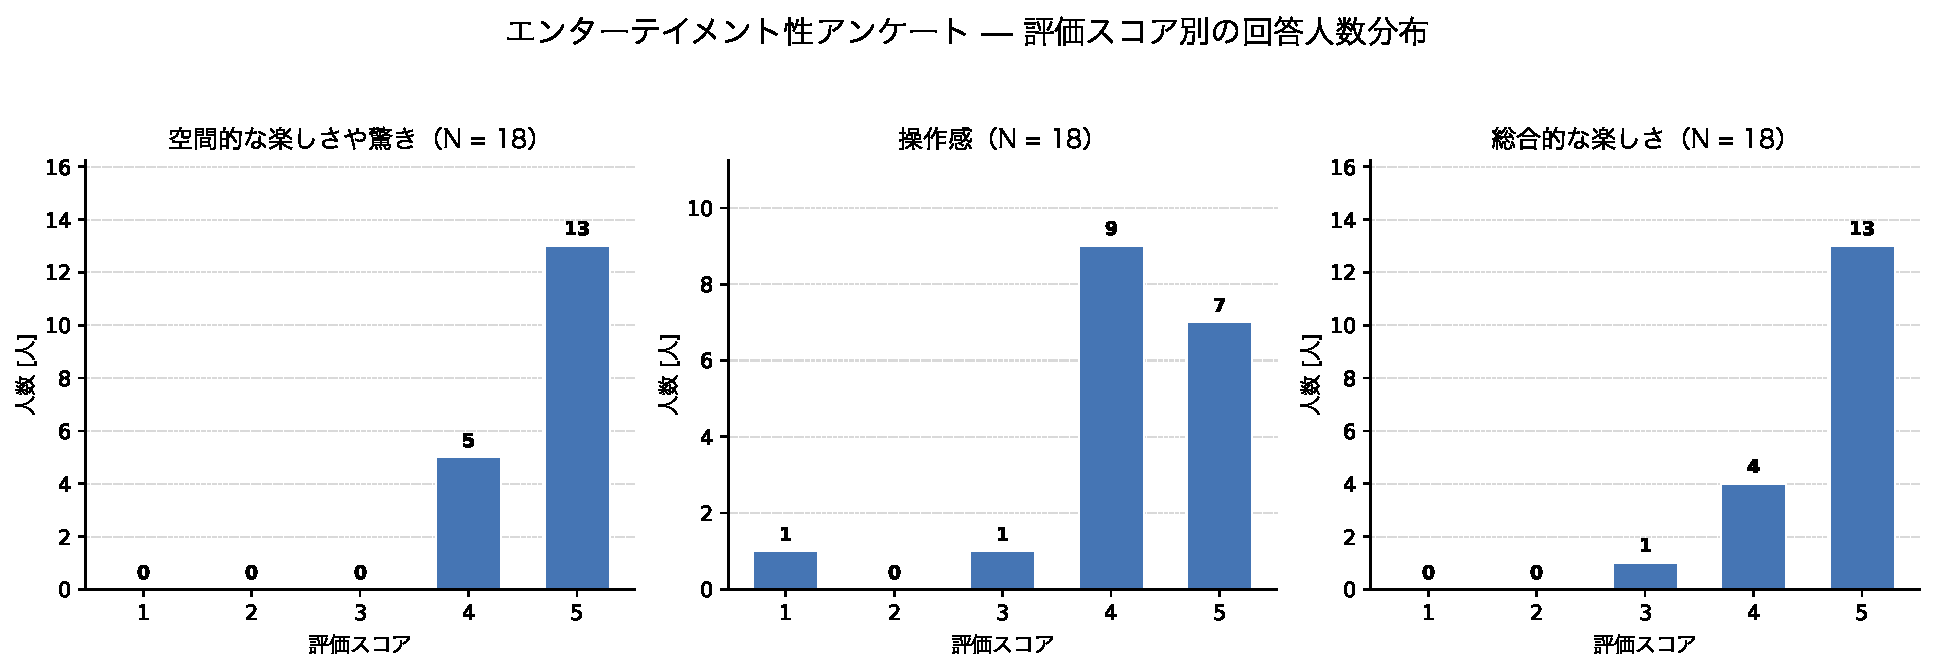
\includegraphics[width=\textwidth]{figs/entertainment_score_histogram.pdf}
    \caption{エンターテイメント性アンケートの評価スコア別の回答人数分布}
    \label{fig:entertainment_score_histogram}
\end{figure}

CSATスコアは，非標準化（点推定のみ）および標準化（95\%Wilson信頼区間\cite{wilson1927}の下限による判定）の両方で算出した．算出結果を表~\ref{tab:csat_entertainment}に，非標準化の結果を図~\ref{fig:csat_entertainment_raw}に，標準化の結果を図~\ref{fig:csat_entertainment_wilson}に示す．

\begin{table}[htbp]
    \centering
    \caption{エンターテイメント性アンケートのCSATスコアとMOP判定結果（MOP目標値75\%）}
    \label{tab:csat_entertainment}
    \resizebox{\textwidth}{!}{%
    \begin{tabular}{lrrrcc}
    \hline
    質問項目 & Top2Box人数 & CSATスコア[\%] & 95\%Wilson信頼区間[\%] & MOP判定（非標準化） & MOP判定（標準化） \\
    \hline
    空間的な楽しさや驚き & 18/18 & 100.0 & [82.4, 100.0] & 達成   & 達成   \\
    操作感               & 16/18 &  88.9 & [67.2,  96.9] & 達成   & 未達成 \\
    総合的な楽しさ       & 17/18 &  94.4 & [74.2,  99.0] & 達成   & 未達成 \\
    \hline
    \end{tabular}%
    }
\end{table}

\begin{figure}[htbp]
    \centering
    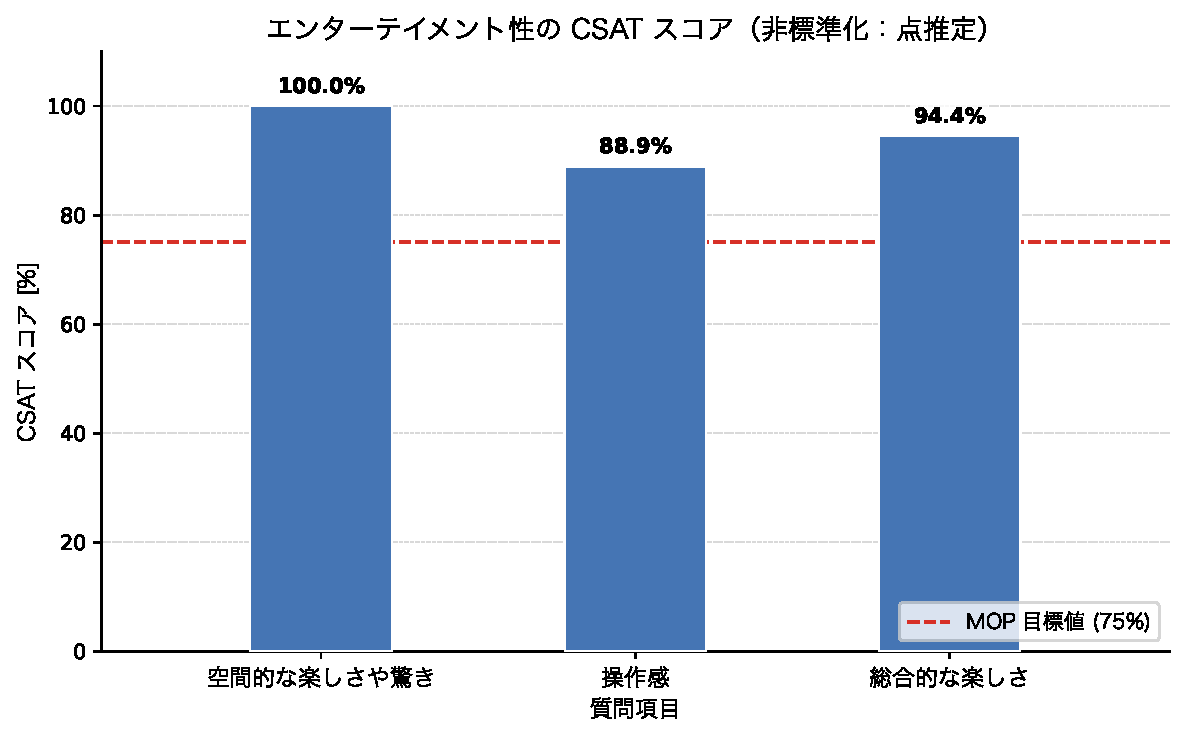
\includegraphics[width=0.85\textwidth]{figs/csat_entertainment_raw.pdf}
    \caption{エンターテイメント性のCSATスコア（非標準化：点推定）とMOP目標値（75\%）の比較}
    \label{fig:csat_entertainment_raw}
\end{figure}

\begin{figure}[htbp]
    \centering
    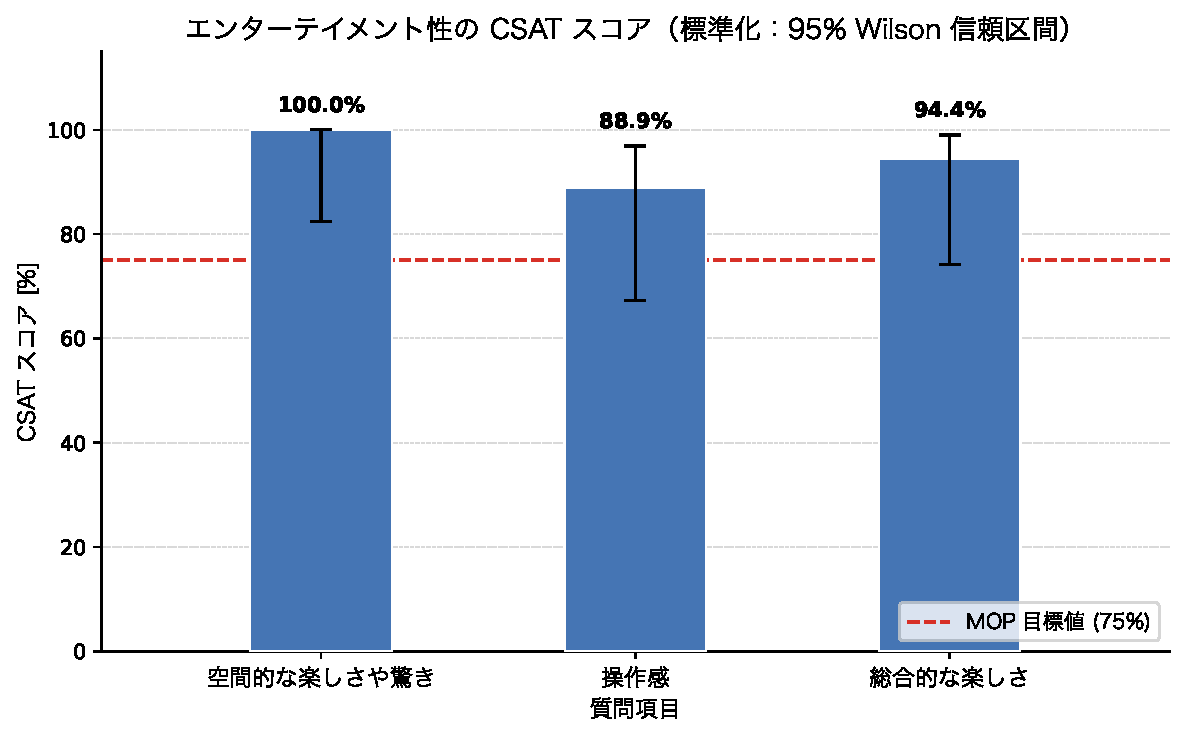
\includegraphics[width=0.85\textwidth]{figs/csat_entertainment_wilson.pdf}
    \caption{エンターテイメント性のCSATスコア（標準化：95\%Wilson信頼区間）とMOP目標値（75\%）の比較}
    \label{fig:csat_entertainment_wilson}
\end{figure}

表~\ref{tab:csat_entertainment}に示す通り，非標準化（点推定）で判定した場合，3項目すべてがMOPの目標値である75\%以上を達成した．特に「空間的な楽しさや驚き」については18名全員が4（満足）または5（大変満足）と回答し，CSATスコアは100.0\%であった．

一方，標準化（95\%Wilson信頼区間の下限による判定）で判定した場合，MOPを達成したのは「空間的な楽しさや驚き」の1項目のみであった．「操作感」および「総合的な楽しさ」は，点推定ではそれぞれ88.9\%，94.4\%であったが，95\%信頼区間の下限値はそれぞれ67.2\%，74.2\%であり，いずれも75\%の目標値を下回った．


\section{考察}
\label{sec:kousatsu}

本システムは，高い没入感を得るために「ユーザの能動的操作」があり，かつ「空間的なフィードバック」があるシステムの作成を目的として設計・評価を実施した．本節では，\ref{sec:hyouka}節で示した単体テストおよび結合テストの結果に基づく考察を行い，実装・評価を通じて確認された本システムのハードウェア依存性を整理した後，評価指標そのものがシステムの有意性を議論する指標として妥当であるかを検討する．続いて，既存システムとの比較および本システムの優位点を整理し，\ref{sec:ketsugo_result}項の末尾で示したハッカソン参加者共通アンケートの結果に基づく考察を行う．本稿の評価は，システムが設計通り動作することを確認する技術的評価（結合テスト）と，利用者からどのように評価されたかを示す主観評価（参加者共通アンケート）の二段階で構成されており，本節ではこの2つを統合して本システムの有効性を検討したうえで，最後に改善案と今後の展望について述べる．

\subsection{単体テストおよび結合テストの結果に関する考察}
\label{sec:kousatsu_test}

\subsubsection{同期確立時間の増大とその要因分析}
\label{sec:kousatsu_douki}

結合テストにおいて，同期開始条件を\SI{50}{ms}以下とした場合，一度同期が確立した後の楽器間の演奏ズレはハース効果\cite{haas1951}に基づくMOPの目標値である\SI{50}{ms}未満に収まった．一方，同期の確立自体に要する時間（ボタン押下から楽曲再生開始までの応答遅延）は，全53回の試行のうち8回がTanらの示す\SI{60}{s}\cite{tan2026}の閾値を超過し，成功率は84.9\%にとどまった．

この2つの同期開始条件の差を比較するため，表\ref{tab:song_start_60ms}および表\ref{tab:song_start_50ms}の測定値をBPM別に図示したものを図\ref{fig:sync_condition_compare}に示す．図\ref{fig:sync_condition_compare}(a)より，\SI{50}{ms}条件の平均応答遅延は全てのBPMで\SI{60}{ms}条件を上回り，標準誤差（エラーバー）も大きい．すなわち，同期開始条件の厳格化は応答遅延を平均的に増大させるだけでなく，試行ごとのばらつきも拡大させている．また，図\ref{fig:sync_condition_compare}(b)より，\SI{60}{s}以内に楽曲再生が開始された試行の割合は\SI{60}{ms}条件では全BPMで100\%である一方，\SI{50}{ms}条件ではBPM60・90・150で低下しており，特にBPM150では50.0\%まで低下した．ただし，同条件の試行数は10回と少なく，BPMに対して単調な傾向も見られないことから，BPMに固有の要因であるかは判別できない．この未達成の要因として，技術的観点から次の2点が考えられる．

\begin{figure}[htbp]
  \centering
  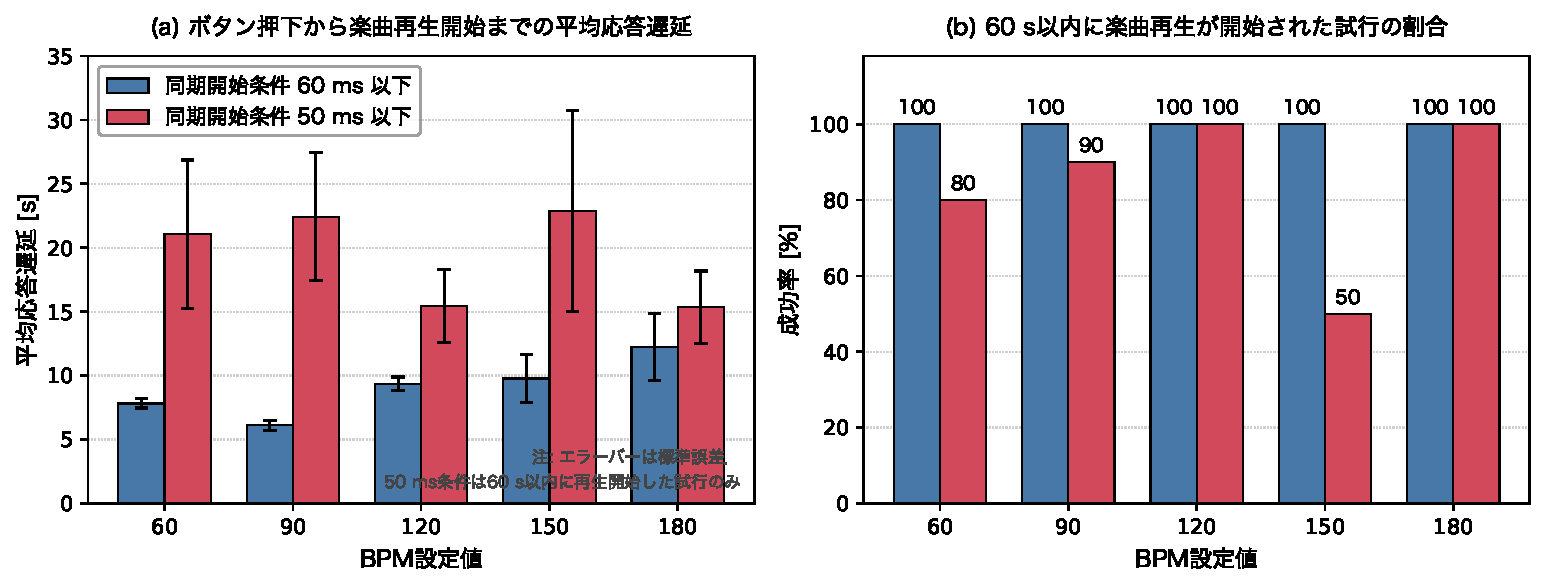
\includegraphics[width=\textwidth]{figs/sync_condition_compare.pdf}
  \caption{同期開始条件（\SI{60}{ms}以下・\SI{50}{ms}以下）別のボタン押下から楽曲再生開始までの応答遅延と成功率の比較}
  \label{fig:sync_condition_compare}
\end{figure}

第一に，同期補正ループの収束特性と許容閾値の関係である．\ref{sec:gakki_naibu}項で述べた通り，本システムの同期確立は，マスターと各スレーブが'R'通信で演奏位置のずれ（diff）を交換し，補正を繰り返した結果，「接続中の全楽器のずれが閾値以内」という条件が成立した時点で完了する．このずれの測定には，往復遅延の半分を片道遅延とみなす近似が用いられているため，測定値には無線通信の遅延変動に由来する誤差が含まれる．許容閾値を\SI{50}{ms}に狭めると，この測定誤差やパケットロスによるずれの揺らぎが閾値幅に対して相対的に大きくなり，全楽器のずれが同時に閾値内へ収まる事象が生じにくくなるため，条件成立までの時間が延びたと考えられる．また，2.4GHz帯の混雑によるUDPパケットロスは，'R'・'O'通信の欠落として補正の機会そのものを減少させる．本テストの実施環境は実演を行ったハッカソン会場そのものではないが，いずれも大学構内という多数のWi-Fi機器が2.4GHz帯を共有する電波環境である点は共通しており，パケットロスが同期確立を遅延させた要因として十分に考えられる．なお，指揮デバイスが指令送信時に行う3周の冗長送信（周間\SI{20}{ms}，\ref{sec:siki_naibu}項）は，演奏開始・終了等の指令を送る一度きりの処理であり，同期確立の補正ループには関与しないため，同期確立時間の増大要因ではない．

第二に，中継機デバイスの回転速度の変動である．\ref{sec:gakki_naibu}項で述べた通り，各楽器デバイスはレーザー光の受光間隔からBPMを推定しており，同期確立の前提として受光間隔が安定している必要がある．しかし，\ref{sec:jissou_kan}項で述べた通り，同一のPWM設定値に対するモータの回転速度は電源電圧の変動等により試行ごとに変動し，さらに\ref{sec:kousatsu_hw}項で述べる光学系の物理的条件によって受光の成立自体が変動する．受光間隔が揺らぐとBPM推定の安定判定に時間を要するため，同期確立時間の試行間のばらつきに寄与したと考えられる．

以上より，\SI{50}{ms}という同期開始条件下での応答遅延の未達成は，ずれ測定の誤差・パケットロスの下で狭い許容閾値を全楽器同時に満たすことの難しさ，および回転速度・受光の物理的な変動に起因するものと考えられる．なお，同期開始条件を\SI{60}{ms}以下に緩和した場合は全25回の試行で成功率100\%，平均応答遅延$\SI{9054.0}{ms}$であり，許容ズレをわずか\SI{10}{ms}緩和するだけで同期確立が安定することから，本システムの同期性能は\SI{50}{ms}という閾値の近傍で動作していると言える．

\subsubsection{ユーザの能動的操作を支える処理成功率の要因分析}
\label{sec:kousatsu_sousa}

ボタン押下による操作反映の成功率は，全160回の試行のうち158回の成功で98.8\%であり，MOPの目標値である99.0\%以上にわずかに届かなかった．失敗した2回の試行はいずれも，モータドライバは動作していたにもかかわらず観覧車が回転しなかった事例である．この要因として，ブレッドボード上の配線の接触不安定が挙げられる．モータドライバまでの信号伝達は正常であったことから，ドライバ出力からモータまでの経路，すなわちブレッドボードのコンタクト部における接触抵抗の一時的な増大により，モータの起動トルクに必要な電流が供給されなかった可能性が高い．また，チャタリング防止のために設けた押下検知後の\SI{300}{ms}の待機処理（\ref{sec:siki_naibu}項）は，待機中の再押下を検出しないため，利用者が短い間隔で操作した場合に微小な検出漏れを生じさせる余地がある．

一方，指揮デバイスの振り動作によるBPM・音量変更の反映成功率は100\%であり，全試行において意図した段階が正しく反映され，多重検知や停止状態での誤反応も確認されなかった．これは，3軸加速度センサの差分算出・多重検知防止・状態反転という段階的な検知ロジック（AccManagerクラス），および可変抵抗器のアナログ値に対する移動平均処理（PotManagerクラス）が，設計通りに機能したことを示している．すなわち，ソフトウェアによる信号処理系は目標を満たす精度で動作しており，未達成の要因はブレッドボード実装というハードウェアの試作段階に固有の物理的要因に集約される．

\subsubsection{音色再現度のばらつきと合成方式の限界}
\label{sec:kousatsu_onshoku}

\ref{sec:tanka_result}項で示した通り，MOS評価に基づく音色再現度のMOP（中央値および最頻値がともに4.0以上）は全6楽器で達成された．一方，回答分布の散らばりに着目すると，ストリングス（評価4以上が90\%）に比べ，ピアノおよびキックドラム（同71\%，74\%）は第1四分位数が3であり，回答の4分の1以上が評価3以下に分布していた．この差の要因は，加算合成を基本とする本システムの音色合成方式の特性から説明できる．

ストリングスやフルートのような持続音系の楽器は，定常的な倍音構造の再現が音色の類似度を支配するため，正弦波の加算合成とビブラート・ノイズ成分の付加によって比較的高い再現度が得られる．これに対しピアノは，打鍵直後の急峻な減衰と，複数弦のわずかなピッチ差に起因するうなり（デチューン）が音色の特徴を決定づける減衰音系の楽器であり，本システムの合成方式ではこれらの時間変化の表現が不足していたと考えられる．また，キックドラムについては，音色の迫力を支配する低域（およそ\SI{100}{Hz}以下）の再生能力が使用したスピーカーの口径・筐体では不足しており，合成波形自体の問題に加えて出力系の物理的制約が評価を低下させたと考えられる．すなわち，ピアノは合成アルゴリズム上の限界，キックドラムは再生装置上の限界という，異なる技術的要因が低評価側への分布の広がりをもたらしたと整理できる．

\subsection{ハードウェア依存性に関する考察}
\label{sec:kousatsu_hw}

本節では，実装および評価の過程で確認された，本システムのハードウェア依存性について考察する．ここでハードウェア依存性とは，システムの動作や性能が，プログラムや設定値のみでは再現されず，個々のハードウェアの状態（部品の個体差，物理的な位置関係，電源の残量等）に依存する性質を指す．本システムがハードウェア依存であると考察する根拠は，次の5点である．

第一に，検知条件の設定を実施のたびにやり直す必要があったことである．\ref{sec:kan_naibu}項で述べた回転速度実測プログラム（LaserIntervalTest）は，周囲光量や取り付け誤差に対応するための適応しきい値方式を採用しているにもかかわらず，実施するごとに検知条件の設定を行う必要があった．これは，環境光・レーザーの照射位置・CdSセルの受光位置といった物理的条件が実施のたびに変化し，一度定めた設定値が再利用できないことを意味する．

第二に，レーザー光の方向と受光素子の位置関係に対する敏感さである．\ref{sec:jissou_jukou}項で述べた通り，レーザー光の方向や受光素子の微細な位置関係によって受光のしやすさが変化するため，デバイスを組み立て直すたびに発泡スチロールによる位置の微調整が必要であり，この調整の結果が同期の成立しやすさを左右した．この位置関係の敏感さを増幅させた要因が，回転部品の歪みである．3Dプリンタで製作した回転リングにはわずかな反り・歪みがあり，リングに取り付けられたレーザーモジュールの照射方向が，リングの回転位置によって変化する．このため，レーザー光の到達位置は8個のモジュール間で一意に定まらず，図\ref{fig:r_cds_angle}に示すように，受光素子側の向きを個別に傾けて合わせ込む対応が必要であった．すなわち，同期性能が光学系の物理的な組み立て状態と部品の成形精度に依存している．

\begin{figure}[htbp]
  \centering
  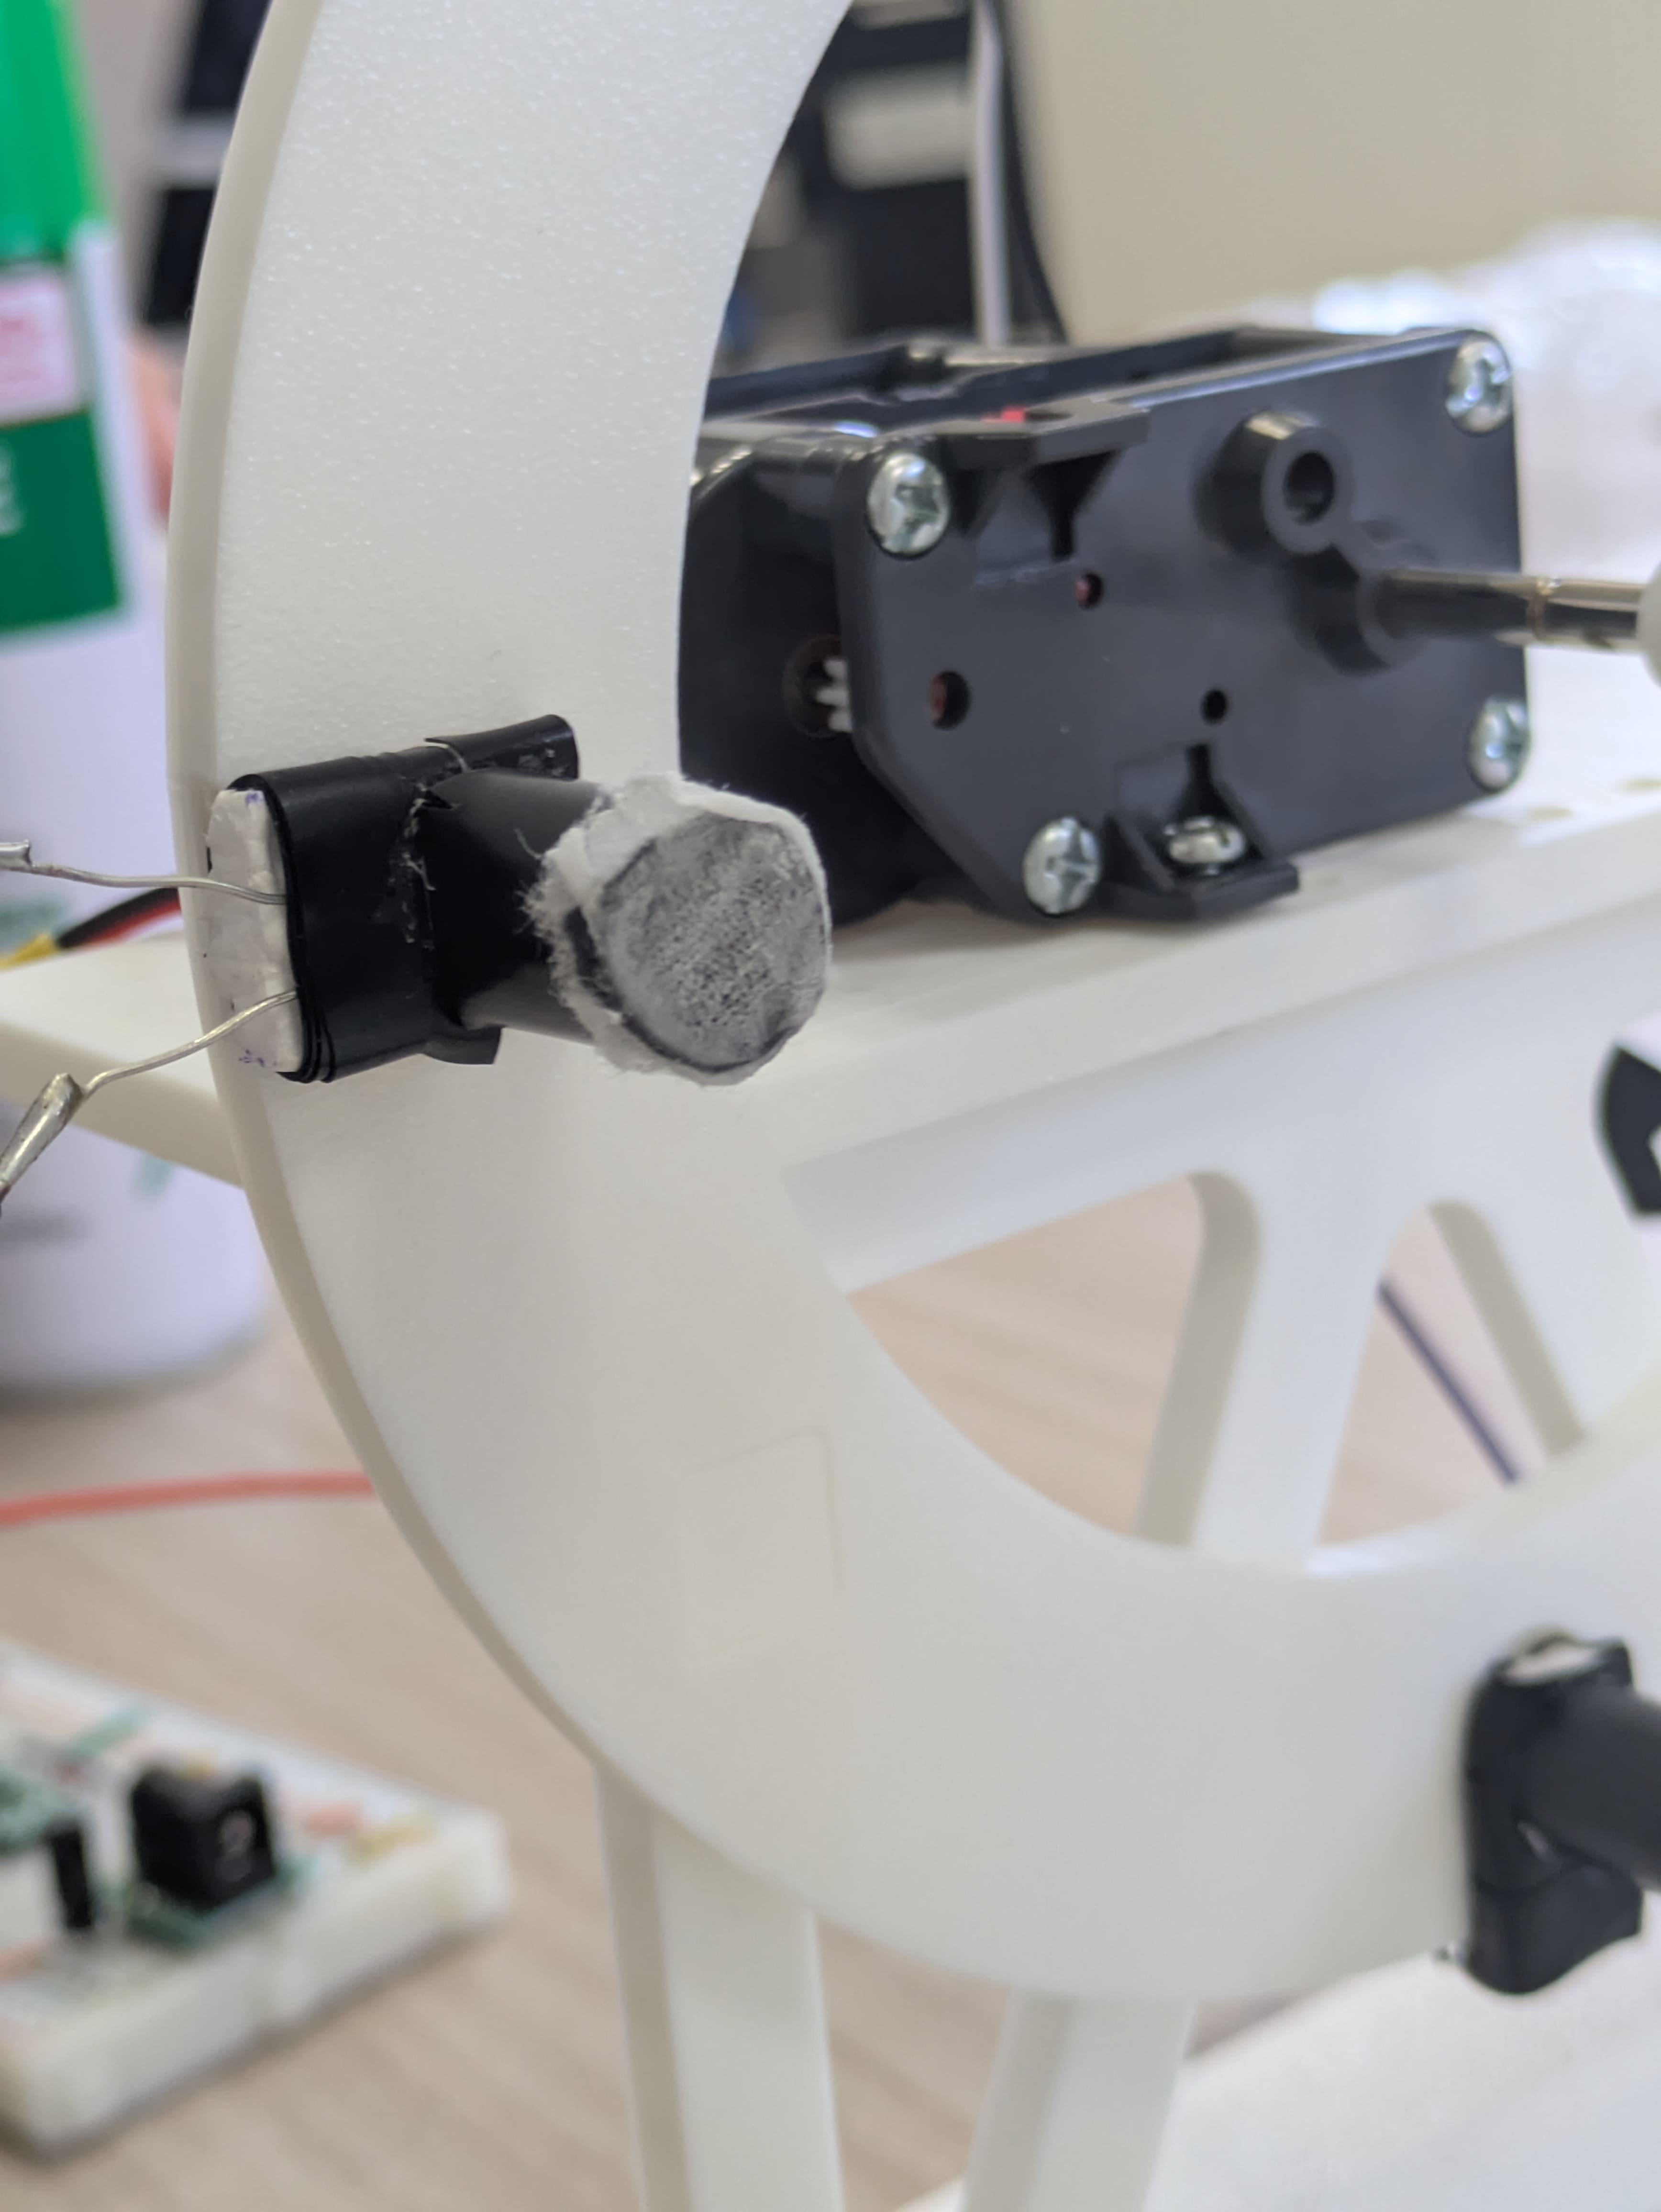
\includegraphics[width=0.55\textwidth]{figs/R_CdS.jpg}
  \caption{受光素子の取り付け角度の調整（回転部品の歪みによりレーザー光の到達方向が一定しないため，受光素子側の向きを個別に傾けて合わせている）}
  \label{fig:r_cds_angle}
\end{figure}

第三に，配線の保守性の低さである．本システムはブレッドボードとジャンパーワイヤーを多用した実装であるため，接触不良が発生した際に，多数の配線の中から断線箇所や接続ミスを特定することに時間を要した．配線経路がはんだ付けやプリント基板によって固定されていないため，故障箇所の切り分けが個々の配線の状態確認に依存する．

第四に，レーザーモジュールの光量が電池の消耗に伴い低下することである．実装では，光量の不足への対策として外部抵抗を除去し，レーザーモジュールに内蔵された回路のみで駆動する構成としたため，電池電圧の低下がそのまま光量の低下として現れる．図\ref{fig:laser_strong_weak}に示す通り，スイッチをONにした直後は受光部に明瞭な輝点が確認できる一方，時間経過後は輝点が減光しており，両者の光量の差は目視でも判別できる．光量の低下は受光時と非受光時の明暗差を縮小させるため，受光検知の成立が電池の残量という時間変化するハードウェア状態に依存する．

\begin{figure}[htbp]
  \centering
  \begin{minipage}{0.48\textwidth}
    \centering
    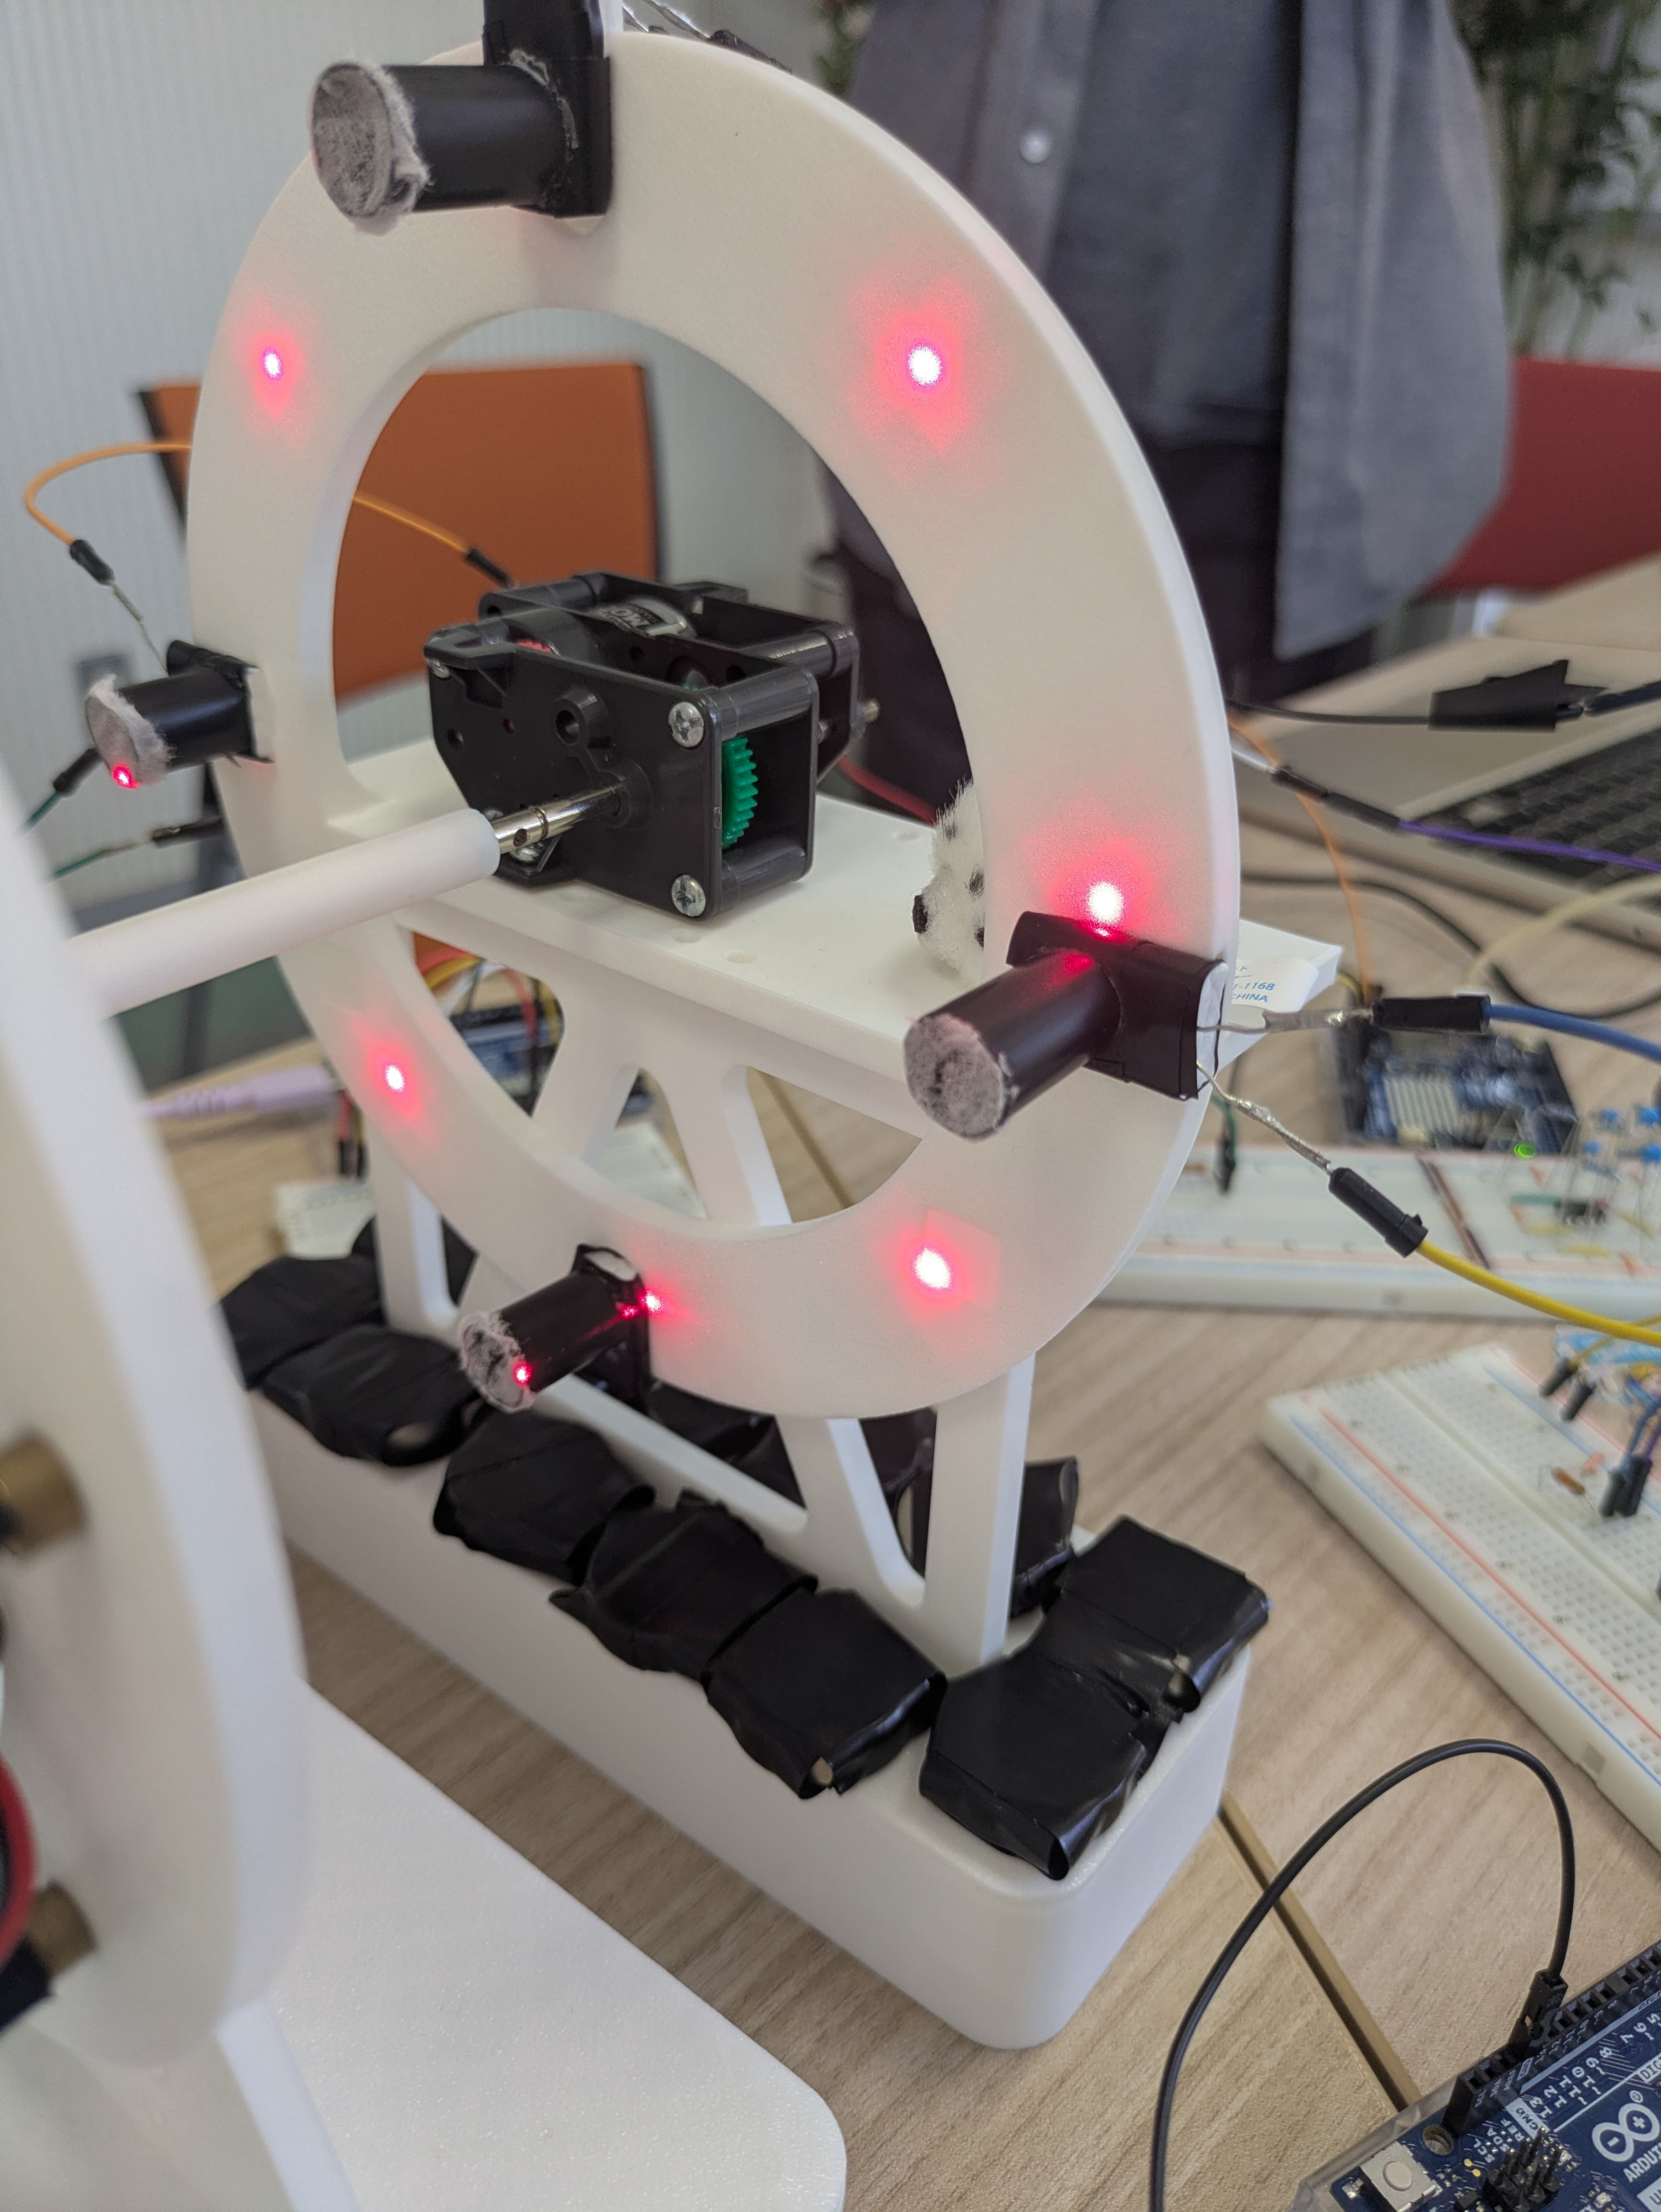
\includegraphics[width=\textwidth]{figs/strong_omote.jpg}
  \end{minipage}
  \hfill
  \begin{minipage}{0.48\textwidth}
    \centering
    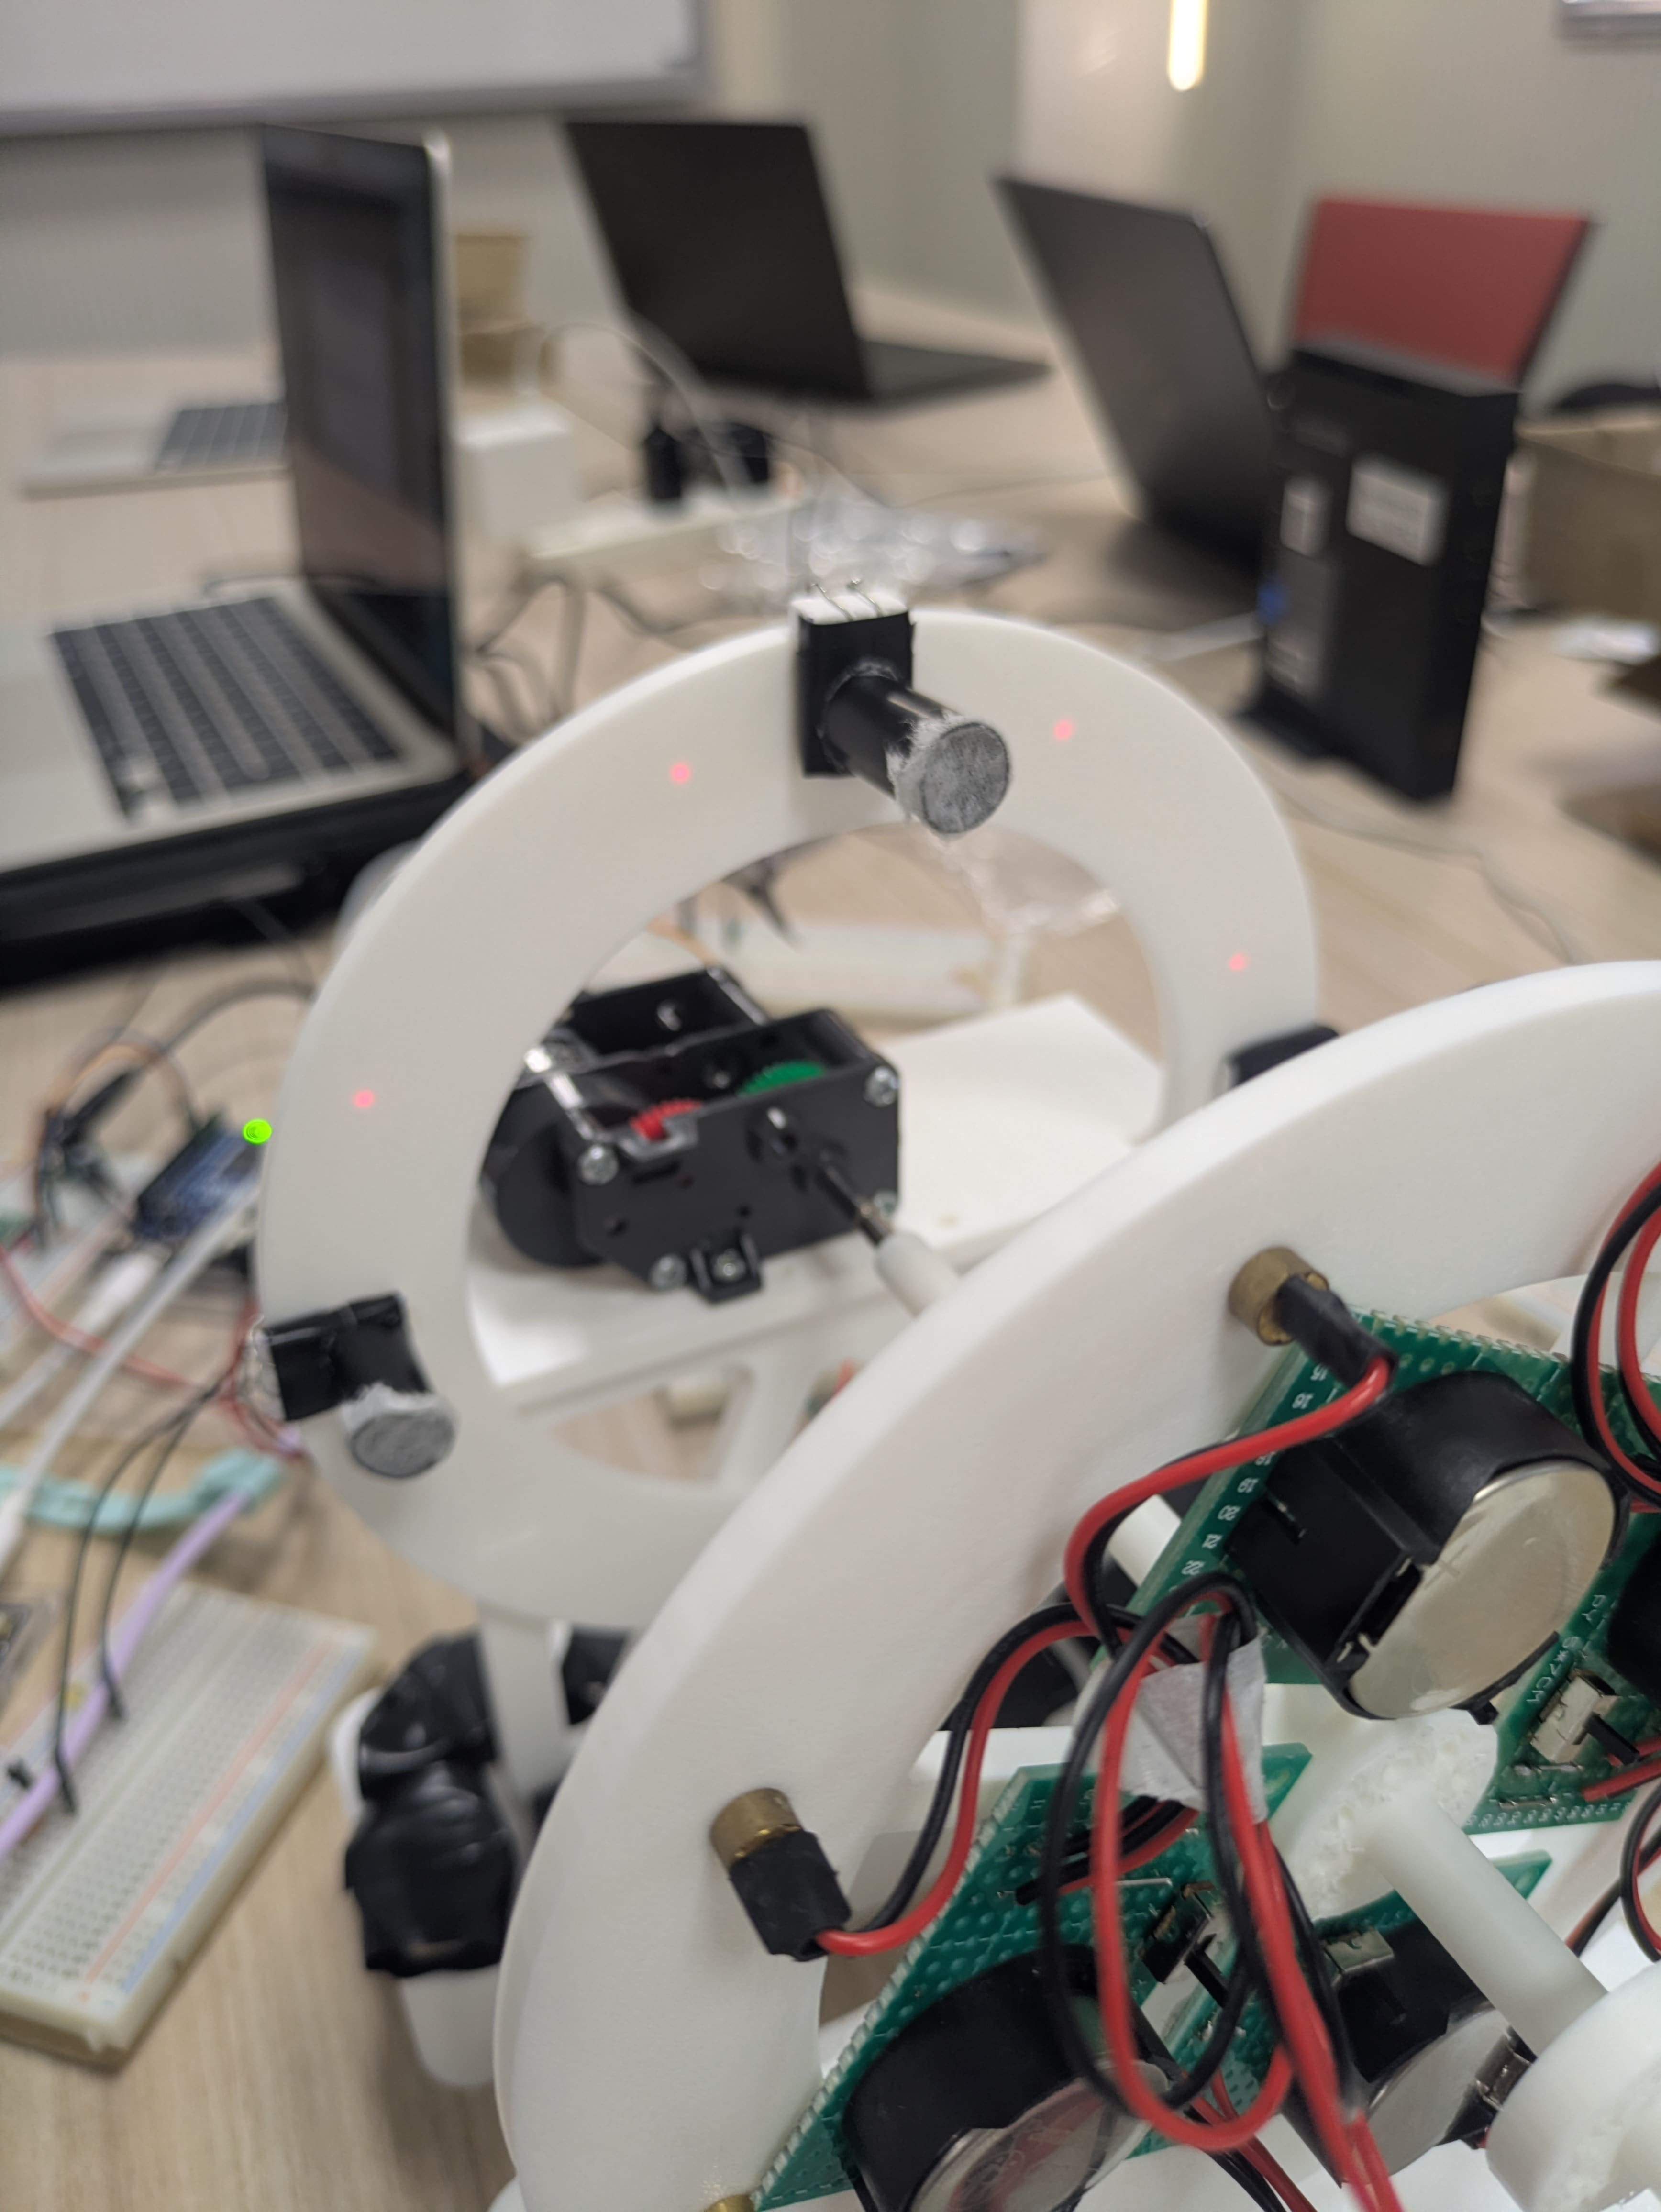
\includegraphics[width=\textwidth]{figs/weak_omote.jpg}
  \end{minipage}
  \caption{電池の消耗に伴うレーザー光量の変化（左：スイッチON直後，右：時間経過後．受光部に投影された輝点の明るさが低下している）}
  \label{fig:laser_strong_weak}
\end{figure}

第五に，ボタン電池の消耗の速さである．回転リング上の8個のレーザーモジュールを演奏中常時点灯させる構成であるため電池の消耗が早く，数時間規模の連続稼働は電池交換なしには維持できなかった．したがって，長時間の展示・実演には電池交換という人手の介入が前提となる．

以上の5点は，いずれも「同一のプログラム・同一の設定値を用いても，ハードウェアの状態が変われば同一の動作が再現されない」という共通の性質を持つ．この性質は，第一に，同一設計から複数の個体を製作した場合や，会場を移して再組み立てした場合に，個体・設置ごとの再調整を必須とするため，システムの再現性・可搬性を制約する．第二に，\ref{sec:jissou_kan}項で述べたモータ特性の試行間変動と同様に，評価テストの試行間で条件が完全には一致しないことを意味し，\ref{sec:hyouka}節で示した測定値のばらつきの一因となった可能性がある．これらの依存性の低減策については\ref{sec:kousatsu_tenbou}項で述べる．

\FloatBarrier

\subsection{評価指標の妥当性に関する考察}
\label{sec:kousatsu_shihyou}

本節では，\ref{sec:hyouka}節で用いた評価指標が，本システムの有意性を議論するための指標として妥当であるかを検討する．

まず，音色再現度テストにMOS評価を採用したことの妥当性について述べる．主観評価の指標としては，CSATスコア（Customer Satisfaction Score：5段階評価のうち4以上の高評価を付けた回答者の割合として算出される顧客満足度の指標）という評価方法もあるが，CSATスコアは回答を「4以上か否か」で二値化するため回答分布の情報の多くを捨てることになり，また目標値として一般に参照される75\%\cite{acsi}は企業の顧客満足度調査の平均値に由来する値であって，音の品質評価という本テストの文脈とは領域が異なる．これに対しMOS評価\cite{itu_p800}は，音声・音響分野において主観品質を測定するために標準化された手法であり，評定値4が「Good」という品質水準に対応づけられているため，「中央値および最頻値が4.0以上」という目標値に領域固有の解釈可能な根拠を与えられる．したがって，評価対象（音色の類似性）と指標の由来する領域（音の主観品質評価）が一致するMOS評価の採用は，CSATスコアよりも妥当性が高いと判断できる．

次に，MOS評価における代表値の選択について述べる．MOS評価は本来，Mean Opinion Score（平均オピニオン評点）という名称の通り評定値の算術平均を代表値とする手法であり，本テストのように$N=100$の規模であれば，中心極限定理（母集団の分布形状によらず，標本数が十分大きいとき標本平均の分布が正規分布に近づくという定理）に基づいて平均値の信頼区間を構成し，平均値が目標値を上回るかを判定する方法も考えられる．しかし本テストでは，次の3つの理由から中央値・最頻値による判定を採用した．第一に，リッカート尺度は順序尺度であり，「3と4の差」と「4と5の差」が等しいことは保証されないため，算術平均の値そのものの解釈が困難である．第二に，回答分布は高評価側に偏った非対称な分布であり（例えばハイハットでは評価5が62\%），このような分布では平均値が回答者の典型的な評定を代表しない．第三に，MOPの目標値4.0は「ある程度似ている」という回答カテゴリに対応しており，中央値・最頻値であれば「過半数の回答者が4以上と評定した」「最も多かった評定が4以上であった」という直接的な解釈が可能である．すなわち，中心極限定理は標本平均の推定精度（信頼区間の妥当性）を保証するものであって，順序尺度上の平均値の解釈可能性を与えるものではないため，本テストの判定には中央値・最頻値が適する．なお，リッカート尺度の順序尺度性を考慮して散らばりを四分位範囲で併記する構成も，尺度水準に整合した処理である．ただし，中央値・最頻値はカテゴリ値であるため楽器間の差異に対する分解能が低く，本稿では四分位数の併記によってこれを補ったが，サンプルサイズに基づく推定の不確実性の定量化（信頼区間に相当する評価）は行っていない点が限界として残る．

次に，応答遅延に関する閾値の妥当性について述べる．Nielsenの\SI{10}{s}\cite{nielsen1993}およびTanらの\SI{60}{s}\cite{tan2026}は，いずれもユーザが注意を維持できる限界を示す閾値であり，「これを超えると体験が破綻する」下限条件としては根拠がある．ただし，これらは注意の維持に関する閾値であって，快適と感じる応答時間の閾値ではない．ボタン押下から中継機デバイスの回転開始までの平均応答時間は$\SI{1005.8}{ms}$であり，\SI{10}{s}の約10分の1でありMOPは達成されたが，Nielsenが「思考の流れを維持できる限界」とする\SI{1.0}{s}\cite{nielsen1993}とほぼ同水準である．したがって，本MOPの達成は体験の破綻がないことを保証するものの，操作の快適性までを保証するものではなく，より厳しい閾値（例えば\SI{1.0}{s}）を採用した場合の達成状況は境界上にあることに留意が必要である．一方，ハース効果に基づく\SI{50}{ms}\cite{haas1951}は聴覚の知覚特性に直接根拠を持つ閾値であり，「複数の楽器デバイスの発音が1つの輪唱として知覚されるか」という本システムのMOEを判定する指標として妥当である．ただし，この指標は定常状態の演奏ズレのみを対象としており，\ref{sec:kousatsu_douki}項で述べた同期確立時間の増大を捉えられない．すなわち，同期の品質（ズレ）と同期の確立コスト（時間）は別個の指標で評価すべきであり，後者に対応するMOPが\SI{60}{s}という粗い閾値しか持たなかったことは，評価設計上の課題である．

最後に，処理成功率99.0\%\cite{kobesoft_availability}という目標値について述べる．この値はWebサービスの稼働率（ツーナイン）に由来するが，成功率98.8\%（158/160）という結果に対して統計的な観点から検討すると，成功率の95\%Wilson信頼区間\cite{wilson1927}は$[95.6\%, 99.7\%]$であり，目標値の99.0\%を区間内に含む．すなわち，160回という試行回数では，真の成功率が99.0\%以上であるか否かを統計的に判別できず，「わずかに未達成」という点推定に基づく判定は，推定の不確実性を考慮すると確定的なものではない．99.0\%という高い目標値の達成を有意に判定するには，数百回以上の試行が必要であり，試行回数の設計と目標値の水準が整合していなかった点は，評価指標の運用上の限界である．

\subsection{既存システムとの比較および優位点}
\label{sec:kousatsu_hikaku}

\ref{sec:hajimeni}節で整理した通り，音楽に視覚的フィードバックを付加する既存システムには，それぞれ異なる限界がある．Yamaha Disklavier ENSPIREシリーズ\cite{yamaha}に代表される自動演奏技術は，鍵盤動作という視覚的フィードバックを備えるが，その提示範囲は楽器本体の周辺に限られ，空間全体には行き渡らない．DMX信号による照明制御\cite{sekine2021}は空間的な演出を実現するが，観客はあらかじめプログラムされた演出を受動的に鑑賞するのみであり，能動的な操作を持たない．ReacTable\cite{reactable}のようなタンジブル・インターフェースは物理操作による能動的な演奏制御を実現するが，視覚的フィードバックは卓上ディスプレイの表示領域内で完結し，第三者や会場全体への共有を想定していない．

本システムは，指揮デバイスによる能動的操作（ボタンによる演奏開始・終了，振り動作と可変抵抗器によるBPM・音量のリアルタイム制御）と，観覧車型デバイスの回転・レーザー光・分散配置された楽器デバイスの発音という空間的フィードバックを同時に備える点で，これらの既存システムのいずれとも構成が異なる．評価結果に基づくと，この構成の優位点は次の2点に整理できる．第一に，操作の反映がボタン押下で98.8\%，振り動作によるBPM・音量変更で100\%と高い成功率で機能しており，能動的操作が実効的に成立していることである．第二に，一度同期が確立した後の楽器間の演奏ズレが\SI{50}{ms}未満に収まっており，物理的に分散した複数の発音体を，聴覚上1つの演奏として成立する精度で協調動作させていることである．画面内の音源定位や単一スピーカーからの再生とは異なり，実空間に分散した音源と可動構造物が同期して動作する点は，既存システムでは提供されない体験であり，\ref{sec:kousatsu_kyoutsuu}項で述べる参加者共通アンケートにおいて「演出の華やかさ」および「楽しさ・高揚感」が全教室平均を有意に上回ったことは，この優位点が利用者の体験として知覚されたことを示唆している．

\subsection{参加者共通アンケートに基づく考察}
\label{sec:kousatsu_kyoutsuu}

本節では，\ref{sec:ketsugo_result}項の末尾で示したハッカソン参加者共通アンケートの結果（表\ref{tab:hackathon_stats}，表\ref{tab:hackathon_welch}，表\ref{tab:hackathon_friedman}）に基づき，本システムの体験としての到達点と課題を考察する．なお，本アンケートは他チームの作品との相対比較であり，本システムの有無による体験の差を比較したものではないため，本節の結果のみをもって本システムの有効性を示すものではない．本節では，本チームの評価とは独立に実施された第三者による客観的評価として，結合テストによるシステム評価を補強する結果と位置付けて考察する．

まず，全教室平均との比較（表\ref{tab:hackathon_welch}）において，「演出の華やかさ」および「楽しさ・高揚感」は，主たる根拠であるMann--WhitneyのU検定で有意に全教室平均を上回り，補助的なWelchのt検定の結果もこれと一致した．効果量（$d=0.84$，$d=0.73$）も大〜中程度の差の大きさを示しており，観覧車の回転・レーザー光・分散した発音体という空間的フィードバックが，演出面の体験として全参加チームの平均水準を上回って知覚されたことを示唆している．一方，「没入感・臨場感」は，平均値としては全教室を上回る向上傾向がみられたものの，主たる根拠であるMann--WhitneyのU検定では統計的な有意差は確認されなかった．補助的なWelchのt検定では有意（$p=0.032$）であったが，正規性が棄却されたデータに対するパラメトリック検定の結果であるため，これのみを根拠に没入感が全参加チームの平均水準を上回ったと断定することはできない．

次に，「一体感・同期の心地よさ」が4項目中唯一，平均値が全教室を下回り，かつチーム40内でも平均値・第1四分位数がともに最も低くSDが最も大きい項目であったという結果は，\ref{sec:kousatsu_douki}項で述べた同期確立時間の課題と整合的である．すなわち，一度同期が確立した後の演奏ズレは\SI{50}{ms}未満に収まっていたものの，同期確立までに最大数十秒を要する場合があり，体験者が観覧した時点によっては同期が確立する前の状態（各楽器デバイスのタイミングが揃っていない状態）を観測した可能性がある．回答分布における低評価側（1〜3）への裾の広がりは，このような体験タイミングの差によって説明できる．空間的な「演出」は高く評価される一方で「同期の心地よさ」が相対的に低いという乖離は，本システムの残された技術課題が同期確立の高速化・安定化にあることを，チーム外の評価者による独立したデータから裏付けるものである．

次に，項目間の比較（表\ref{tab:hackathon_friedman}）の結果から，チーム40の評価は「演出・楽しさ」が高く「没入感・一体感」が相対的に低いという2群の構造を持つことが分かる．演出面の刺激としての評価が，没入感・一体感という体験の深さに関する評価を有意に上回っているこの構造は，全教室比較の結果と合わせて，空間的フィードバックの演出効果は十分に機能した一方，同期の品質に関わる体験とそれを介した没入感には改善の余地があることを示している．

最後に，以上の結果を結合テストの結果と統合して本システムの有効性を検討する．技術的評価である結合テスト（\ref{sec:ketsugo_result}項）では，一度同期が確立した後の演奏ズレが\SI{50}{ms}未満に収まる同期演奏，98.8\%〜100\%の操作反映，およびBPM・音量のリアルタイム制御が，設計通りに動作することを確認した．これに対し主観評価である参加者共通アンケートでは，第三者による客観的評価として，「演出の華やかさ」および「楽しさ・高揚感」が全教室平均を有意に上回った．結合テストおよび参加者評価を総合すると，本システムは指揮動作に応じた空間演出を実現し，体験価値の向上に寄与するシステムとして有効であると考えられる．一方，「没入感・臨場感」および「一体感・同期の心地よさ」については統計的な有意差が確認されなかったため，本稿ではこれらに対する効果を断定せず，同期確立の高速化・安定化とあわせて今後の課題とする．

\subsection{改善案と今後の展望}
\label{sec:kousatsu_tenbou}

以上の考察に基づき，本システムの改善案を技術的課題ごとに述べる．

第一に，同期確立時間の短縮である．現行の一律3周の冗長送信は，パケットロスの有無にかかわらず固定のオーバーヘッドを発生させる．これに対し，受信側からの確認応答（ACK）に基づく選択的再送方式へ変更すれば，パケットが正常に到達している場合の送信回数を1回に削減でき，電波状況に応じて冗長度を動的に調整することも可能となる．また，同期確立を条件成立の待機ではなく，事前の時刻同期（各デバイス間のクロックオフセットを往復遅延から推定する方式）に基づく開始時刻の指定へ置き換えることで，同期確立時間をBPMや電波状況に依存しない一定値に近づけられると考えられる．物理層の対策としては，Arduino UNO R4 WiFiの無線部が2.4GHz帯のみの対応であることを踏まえ，混雑の少ないチャネルの事前調査・固定や，会場環境によっては有線（シリアルまたはRS-485等）による同期線の追加が有効である．

第二に，電気的な安定性の向上である．指揮デバイスで確認されたI2Cバスのロックアップに対しては，I2C配線の短縮・プルアップ抵抗の適正化・はんだ付けによる基板化により，ノイズや接触不良に起因するバス異常の発生自体を抑制することが望ましい．現行のソフトウェアによるバス復旧処理は有効に機能したが，復旧処理中は加速度検知が前回値で代替されるためである．また，中継機デバイスのモータがブラシ接点で発生させる電気ノイズおよび電源変動に対しては，既設の\SI{0.01}{\micro\farad}コンデンサに加えて，スナバ回路\cite{ieice_knowledgebase}の挿入やモータ系と制御系の電源分離が，回転速度の安定化（\ref{sec:kousatsu_douki}項で述べた受光間隔の揺らぎの低減）に有効と考えられる．

第三に，ボタン操作の反映成功率の改善である．失敗事例の要因がブレッドボードの接触不安定にあることから，はんだ付けによるユニバーサル基板またはプリント基板への移行が最も直接的な対策である．また，\SI{300}{ms}の待機によるチャタリング防止を，RCフィルタとシュミットトリガによるハードウェアデバウンスと割り込み駆動の検知へ置き換えることで，待機中の検出漏れを排除できる．これらの対策のうえで，99.0\%という目標値の達成を統計的に判定するためには，\ref{sec:kousatsu_shihyou}項で述べた通り数百回規模の試行回数を確保する必要がある．

第四に，\ref{sec:kousatsu_hw}項で述べたハードウェア依存性の低減である．配線の保守性に対しては，ボタン操作の対策と同様に，はんだ付けによる基板化で配線経路を固定することにより，接触不良の発生自体を抑えるとともに故障箇所の特定を容易にできる．光学系の位置依存に対しては，レーザーと受光素子の位置決めを手作業の微調整に委ねるのではなく，3Dプリント部品にガイド（位置決め用の溝や穴）を一体成形し，組み立てのたびに同一の位置関係が機械的に再現される構造とすることが有効である．検知条件の設定については，起動時に一定時間の計測を行って閾値を自動決定する較正処理を組み込むことで，実施ごとの手動設定を不要にできる．電源に対しては，レーザーモジュールの駆動に昇圧・定電圧回路（電池電圧が低下しても一定の出力電圧を維持する回路）を追加して光量を電池残量から切り離すこと，および容量の大きい電池または充電式電池への変更により連続稼働時間を延長することが考えられる．

第五に，音色再現度の改善である．ピアノについては，打鍵直後の急峻な減衰を表現するエンベロープの精緻化と，複数弦のピッチ差を模擬したデチューン（わずかに周波数をずらした正弦波の重畳によるうなりの生成）の導入が有効と考えられる．キックドラムについては，合成波形の改善に加えて，低域再生能力の高い大口径スピーカーまたはエンクロージャの採用という出力系の改善が必要である．

最後に，評価方法の展望である．本稿の評価は，音色再現度をMOS評価により音の主観品質評価として標準的な枠組みに整合させ，参加者共通アンケートについては正規性検定の結果に基づきノンパラメトリック検定（Mann--WhitneyのU検定，Friedman検定，Wilcoxonの符号付き順位検定）を適用した．一方，音色再現度テストにおけるサンプルサイズに基づく不確実性の定量化（中央値・最頻値に対する信頼区間に相当する評価）は今後の課題として残っている．また，参加者共通アンケートで示唆された「同期の心地よさ」の課題を検証するためには，同期確立前後の体験を区別した評価設計（体験タイミングの統制）が必要である．これらを整備することで，改善施策の効果を統計的に判定可能な形で追跡できると考えられる．

\FloatBarrier

\section{おわりに}
\label{sec:owarini}

本稿では，回転機構のレーザー受光と楽器間無線通信による同期・輪唱システムの設計・実装・評価について報告した．本節では，プロジェクトで実現できた内容と残された課題を整理し，\ref{sec:hajimeni}節で示した目的との対応関係を述べる．

\ref{sec:hajimeni}節では，デジタル配信では代替できないライブ体験の価値が，同じ空間を共有しているという感覚に由来するという知見に基づき，既存の自動演奏技術が持つ「多感覚的フィードバック」と「空間全体への共有」の不足という課題を指摘した．そのうえで，ユーザの能動的操作を受け付ける指揮デバイス，空間全体へ視覚的フィードバックを共有する観覧車型の中継機デバイス，および分散配置された楽器デバイスの3種で構成されるシステムにより，会場全体を巻き込む没入感の高い演奏体験を提供することを目的として設定した．

この目的に対し，本プロジェクトで実現できた内容は次の通りである．第一に，能動的操作の実現である．ボタン押下による演奏の開始・終了，指揮デバイスの振り動作および可変抵抗器によるBPM・音量のリアルタイム変更を実装し，\ref{sec:hyouka}節の評価において，振り動作によるBPM・音量変更は反映成功率100\%，ボタン押下は成功率98.8\%・平均応答時間約\SI{1.0}{s}で動作することを確認した．第二に，空間的フィードバックの実現である．観覧車型デバイスの回転とレーザー受光による発音制御を実装し，物理的に分散した複数の楽器デバイスを，一度同期が確立した後はハース効果の許容限界である\SI{50}{ms}未満の演奏ズレで協調動作させた．これは，複数の発音体が聴覚上1つの輪唱として知覚される精度である．第三に，音色再現の実現である．6種の楽器音を合成し，MOS評価に基づく音色再現度のMOP（中央値および最頻値がともに4.0以上）を全楽器で達成した．さらに，本チームの評価とは独立に実施された参加者共通アンケートにおいて，「演出の華やかさ」および「楽しさ・高揚感」が全参加チームの平均を有意に上回ったことは，能動的操作と空間的フィードバックの組み合わせという本システムの構成が，体験として実際に機能したことを裏付けている．

一方，残された課題も評価を通じて明確になった．第一に，同期確立時間の課題である．同期開始条件を\SI{50}{ms}以下とした場合，同期の確立自体に長時間を要し，応答遅延のMOPを満たせない試行が生じた．この要因は，パケットロス対策としての冗長送信と同期確立時間とのトレードオフ，およびモータ由来の電気的ノイズにあると分析した．第二に，体験としての「同期の心地よさ」の課題である．参加者共通アンケートにおいて「一体感・同期の心地よさ」は唯一全体平均を下回り，項目間の比較でも「演出・楽しさ」に対して有意に低い評価にとどまった．没入感についても，平均値としては全体を上回る傾向がみられたものの，順位に基づく検定では有意差を確認できなかった．すなわち，空間的フィードバックの演出面の効果は明確に確認された一方，序論で目的とした没入感の向上は部分的な達成にとどまり，その隘路が同期確立の高速化・安定化にあることが，技術的評価と体験評価の両面から一貫して示された．第三に，実装・評価上の課題として，ブレッドボード実装に起因する操作反映の不安定さ，レーザー光量の電池残量への依存や光学系の位置調整に代表されるハードウェア依存性，ピアノ・キックドラムの音色再現のばらつき，および試行回数と目標値の水準の不整合といった評価設計の限界が残っている．

以上を総括すると，本プロジェクトは，能動的操作と空間全体で共有される物理的フィードバックを兼ね備えた演奏システムを実装し，その演出効果を定量的な評価によって実証した点で，序論で示した目的を大きく前進させた．同時に，没入感の完全な達成には，利用者がいつ体験しても同期した演奏に接することができる同期確立の即時性が不可欠であることを明らかにした．\ref{sec:kousatsu}節で述べた確認応答に基づく再送方式や時刻同期方式への変更，ノイズ対策，基板実装への移行といった改善を施したうえで，同期確立前後の体験を統制した評価を行うことが，会場全体を巻き込む没入感の高い演奏体験の完成に向けた次の段階である．



\newpage


\newpage
\begin{thebibliography}{99}
    \bibitem{cul} 株式会社マーケットリサーチセンター，``音楽出版の日本市場（～2031年）、市場規模（パフォーマンス、同期、デジタル収益）・分析レポートを発表,'' \url{https://www.atpress.ne.jp/news/4436457}，2026/4/22参照.
    \bibitem{live} LP Information，``ライブコンサート市場占有率分析レポート,'' \url{https://www.atpress.ne.jp/news/3304316}，2026/4/22参照.
    \bibitem{acpc} 一般社団法人コンサートプロモーターズ協会，``ライブ市場調査　基礎推移表'' \url{https://www.acpc.or.jp/marketing/transition/}，2026/5/18参照.
    \bibitem{taniguchi2019} 谷口由貴，``ストリーミングサービスが生み出した新たな音楽消費サイクル,'' 博報堂 The Hakuhodo，\url{https://www.hakuhodo.co.jp/magazine/61505/}，2019/9/12，2026/7/7参照.
    \bibitem{Kreuzer2025} Martin Kreuzer, Melanie Wald-Fuhrmann, Christian Weining, Martin Tr\"{o}ndle, and Hauke Egermann, ``Western Classical Music Concerts Are More Immersive, Intellectually Stimulating, and Social, When Experienced Live Rather Than in a Digital Stream: An Ecologically Valid Concert Study on Different Modes of Liveness,'' \textit{Music \& Science}, vol.8, 2025.
    \bibitem{Natalia2018} Natalia Cooper, Dimitrios Mileounis, Patrick Williams, and Frank P. Brooks,``The effects of substitute multisensory feedback on task performance and the sense of presence in a virtual reality environment,''\textit{PLOS ONE},vol.13,no.2,p.e0191846,2018.
    \bibitem{Martin} Martin, R., and Nielsen, N. Enacting Musical Aesthetics: The Embodied Experience of Live Music. Music \& Science, 7,2024
    \bibitem{yamaha} Yamaha Music Japan，``ENSPIRE PRO,'' \url{https://jp.yamaha.com/products/musical_instruments/pianos/disklavier/enspire_pro/features.html#product-tabs}，2026/5/19参照.
    \bibitem{sekine2021} 関根 伸也，``DMX512信号システムなどの現状技術,'' 電気設備学会誌，vol.41，no.72026，p.382-385，2021
    \bibitem{reactable} ReacTable Legacy，``Welcome|ReacTable Legacy,'' \url{https://reactable.com/}，2026/5/19参照.
    \bibitem{ref:control}
    Control.com, ``DC Motor Speed Control,'' {\em Lessons In Electric Circuits}, \\
    \url{https://control.com/textbook/variable-speed-motor-controls/dc-motor-speed-control/}，（参照 2026-05-04）．
    \bibitem{laser} 秋月電子通商，``fu650ad5-c6 データシート,'' \url{https://akizukidenshi.com/goodsaffix/fu650ad5-c6.pdf}，(参照 2026-06-30).
    \bibitem{ieice_knowledgebase}関根正興，``スナバ回路,''電子情報通信学会 知識ベース，8群--5編--2章 2-4-2，2019．
    \bibitem{haas1951} H. Haas, ``\"{U}ber den Einfluss eines Einfachechos auf die H\"{o}rsamkeit von Sprache,'' \textit{Acustica}, vol.1, no.2, pp.49--58, 1951.
    \bibitem{kobesoft_availability} KOBESOFT，``稼働率,'' \url{https://kobesoft.co.jp/mikata/words/network-cloud/availability-rate/}，(参照 2026-05-19)．
    \bibitem{acsi} American Customer Satisfaction Index，``U.S. Overall Customer Satisfaction,'' \url{https://theacsi.org/the-acsi-difference/us-overall-customer-satisfaction/}，(参照 2026-05-17)．
    \bibitem{nielsen1993}J.~Nielsen,``Response Times: The 3 Important Limits,''in \textit{Usability Engineering},Morgan Kaufmann, San Francisco, 1993, pp.~135--137.\url{https://www.nngroup.com/articles/response-times-3-important-limits/}
    \bibitem{tan2026}F.~F.-Y.~Tan and O.~Nov,``Counting the Wait: Effects of Temporal Feedback on Downstream Task Performanceand Perceived Wait-Time Experience during System-Imposed Delays,''
    in \textit{Proceedings of the 2026 CHI Conference on Human Factors in Computing Systems(CHI~'26)},Barcelona, Spain, Apr.~2026, pp.~1--17.\url{https://doi.org/10.1145/3772318.3790475}
    \bibitem{wilson1927} E.~B.~Wilson, ``Probable Inference, the Law of Succession, and Statistical Inference,'' \textit{Journal of the American Statistical Association}, vol.22, no.158, pp.209--212, 1927.
    \bibitem{itu_p800} ITU-T, ``Methods for subjective determination of transmission quality,'' Recommendation P.800, International Telecommunication Union, Geneva, 1996.
    \bibitem{shapiro1965} S.~S.~Shapiro and M.~B.~Wilk, ``An Analysis of Variance Test for Normality (Complete Samples),'' \textit{Biometrika}, vol.52, no.3/4, pp.591--611, 1965.
    \bibitem{welch1947} B.~L.~Welch, ``The Generalization of `Student's' Problem when Several Different Population Variances are Involved,'' \textit{Biometrika}, vol.34, no.1/2, pp.28--35, 1947.
    \bibitem{cohen1988} J.~Cohen, \textit{Statistical Power Analysis for the Behavioral Sciences}, 2nd ed., Lawrence Erlbaum Associates, Hillsdale, NJ, 1988.
\end{thebibliography}



\appendix
\renewcommand{\thefigure}{A.\arabic{figure}} % 図番号を A.1, A.2 に
\renewcommand{\thetable}{A.\arabic{table}}   % 表番号も変える場合
\renewcommand{\theequation}{\Alph{section}.\arabic{equation}} %式番号をA.1, A.2に

\section{指揮デバイスのプログラムソース}
\label{sec:apndx_siki}
本節では，指揮デバイスの制御プログラムの全文を示す．ファイル構成は\ref{sec:siki_naibu}節の表\ref{table:siki_files}の通りである．

\subsection{Controller\_simultaneous.ino}
\begin{lstlisting}[caption={Controller\_simultaneous.ino}, label={lst:siki_ino}]
#include "SyncManager.h"
#include "PotManager.h"
#include "AccManager.h"

#include <Wire.h>
#include <math.h>

// Wi-Fi のネットワーク名(hackathon001-WPA2)
const char SSID[] = "hackathon001-WPA2";
// その Wi-Fi のパスワード(hackathon001)
const char PASS[] = "hackathon001";

const uint8_t input_PIN = 3; // スイッチの状態を読み取るピン
bool switch_status;// ボタンの状態を保持
bool before_switch_status = 0;// 前回のボタンの状態を保持
bool isButtonPlaying = false;// 開始・停止信号を交互に切り替えるフラグ

SyncManager sync;
PotManager pot;
AccManager acc;

void setup() {
    Serial.begin(115200);
    while (!Serial) {}

    Serial.println("--- Setup Started ---");
    pinMode(input_PIN, INPUT);

    Serial.println("Attempting to connect to WiFi...");
    sync.begin(SSID, PASS);

    Serial.println("\nWiFi Connected successfully!");
    Serial.println("Commands: button -> Start/End");

    acc.setupADXL345();

    before_switch_status = digitalRead(input_PIN);
}

void loop() {
    button();
    pot.update();
    acc.update(sync, pot);
}

// 物理ボタンの押下を検知し，開始信号・停止信号のトグル送信と演奏状態フラグの反転を一括管理する．
void button() {
    switch_status = digitalRead(input_PIN);
    if (switch_status == 0 && before_switch_status == 1) {
        if (isButtonPlaying) {
            Serial.println("Button: [END] sending UDP...");
            sync.sendEnd();
            isButtonPlaying = false;
        } else {
            Serial.println("Button: [START] sending UDP to all simultaneously...");
            uint8_t step = pot.getBpmStep();
            sync.sendStart(step);
            isButtonPlaying = true;
        }
        delay(300); // チャタリング防止
    }
    before_switch_status = switch_status;
}
\end{lstlisting}

\subsection{AccManager.h}
\begin{lstlisting}[caption={AccManager.h}, label={lst:siki_acc_h}]
// 加速度センサー管理クラス
#ifndef ACC_MANAGER_H
#define ACC_MANAGER_H

#include <Arduino.h>
#include <Wire.h>
#include "SyncManager.h"
#include "PotManager.h"

class AccManager {
public:
    AccManager();
    // ADXL345（加速度センサー）のI2C初期化および計測開始の準備を行う．
    void setupADXL345();  
    // 20ms周期の時間管理と，閾値判定による指揮棒のシェイク動作検知を行う．
    void update(SyncManager& sync, PotManager& pot); 
    // potの予約フラグを確認し，変化があればsyncを通じてBPMや音量の段階番号を送信する．
    void updateShakedInfo(SyncManager& sync, PotManager& pot);

private:
    float readAccMagnitude(); // I2Cで読み取ったXYZの3軸生データから合成ベクトル(加速度)を算出
    void  recoverI2C(); // I2Cバスロックアップ(切断やノイズなどによりI2C通信が不能になったとき)からの復旧を行う．

    const uint8_t ADXL345_ADDR = 0x53; // 加速度センサー(ADXL345)のI2Cアドレスを定義
    const uint8_t REG_POWER_CTL = 0x2D; // 加速度センサの電源管理をするスイッチを定義
    const uint8_t REG_DATA_FORMAT = 0x31; // 測定範囲設定用レジスタのアドレスを定義
    const uint8_t REG_DATAX0 = 0x32; // 測定した値が書き込まれる場所を定義

    const float accThreshold = 110.0f; // 振ったと判断するための変化量の閾値を定義
    const unsigned long shakeInterval = 750; // 連続検知を防止するための待機時間を定義
    const unsigned long ACC_SAMPLE_INTERVAL = 20;// 加速度センサのサンプリング周期を定義

    // 内部変数
    float currentAccVal = 0.0f; // 加速度センサからの値を格納
    float lastAccVal = 0.0f;  // 変化量算出のための直前の加速度センサ値を格納
    unsigned long lastDetectTime = 0;  // 前回振ったことを検知した時間をms単位で格納
    unsigned long lastSampleTime = 0;// 加速度センサの読み取り間隔を管理するための前回の時刻を格納
    unsigned long lastRecoverMs  = 0;    // 復旧ログ処理の連続実行を防ぐための時刻を保持

    // 振られたときに反転
    bool isStarted = false; 
};

#endif
\end{lstlisting}

\subsection{AccManager.cpp}
\begin{lstlisting}[caption={AccManager.cpp}, label={lst:siki_acc_cpp}]
#include "AccManager.h"

AccManager::AccManager(){
  // コンストラクタ（初期化処理なし）
}

// ADXL345（加速度センサー）のI2C初期化および計測開始の準備を行う．
void AccManager::setupADXL345() {
  Wire.begin();

  Wire.beginTransmission(ADXL345_ADDR);
  Wire.write(REG_POWER_CTL);
  Wire.write(0x08); // Measure bit ON
  Wire.endTransmission();

  Wire.beginTransmission(ADXL345_ADDR);
  Wire.write(REG_DATA_FORMAT);
  Wire.write(0x00);
  Wire.endTransmission();

  lastAccVal = readAccMagnitude();
  
  Serial.println("GY-291 初期化完了");
  Serial.print("閾値: "); 
  Serial.print(accThreshold);
  Serial.print("インターバル: "); 
  Serial.print(shakeInterval); 
  Serial.println(" ms");
}

// 20ms周期の時間管理と，閾値判定による指揮棒のシェイク動作検知を行う．
void AccManager::update(SyncManager& sync, PotManager& pot) {
  unsigned long now = millis();
  
  if (now - lastSampleTime >= ACC_SAMPLE_INTERVAL) {
    lastSampleTime = now;

    currentAccVal = readAccMagnitude();
    float diff = fabsf(currentAccVal - lastAccVal);

    bool overThreshold  = (diff > accThreshold);
    bool intervalPassed = ((now - lastDetectTime) >= shakeInterval);

    // 500msごとにdiff値を表示（閾値チューニング用）
    static unsigned long lastDebugTime = 0;
    if (now - lastDebugTime >= 500) {
      lastDebugTime = now;
      //Serial.print("[ACC] diff="); Serial.print(diff, 1);
      //Serial.print(" / 閾値="); Serial.println(accThreshold, 1);
    }

    if (overThreshold && intervalPassed) {
      lastDetectTime = now;
      isStarted = !isStarted;

      Serial.print("[SHAKE検知] diff=");
      Serial.print(diff, 4);
      Serial.println(isStarted ? " | START送信" : " | END送信");

      updateShakedInfo(sync, pot);
    }

    lastAccVal = currentAccVal;
  }
}

// I2Cで読み取ったXYZの3軸生データから合成ベクトル(加速度)を算出する．
float AccManager::readAccMagnitude() {
  Wire.beginTransmission(ADXL345_ADDR);
  Wire.write(REG_DATAX0);
  // endTransmission!=0 はNACK/バス異常。リピーテッドスタート前に検出する。
  if (Wire.endTransmission(false) != 0) {
    recoverI2C();
    return lastAccVal;   // 直前値を返してニセshakeを防ぐ
  }

  uint8_t n = Wire.requestFrom(ADXL345_ADDR, (uint8_t)6, (uint8_t)true);
  if (n < 6) {             // 6バイト読めない＝ロックアップ等
    recoverI2C();
    return lastAccVal;
  }

  int16_t rawX = (int16_t)((Wire.read()) | (Wire.read() << 8));
  int16_t rawY = (int16_t)((Wire.read()) | (Wire.read() << 8));
  int16_t rawZ = (int16_t)((Wire.read()) | (Wire.read() << 8));

  float fx = (float)rawX;
  float fy = (float)rawY;
  float fz = (float)rawZ;

  return sqrtf(fx * fx + fy * fy + fz * fz);
}

// I2Cバスロックアップ(切断やノイズなどによりI2C通信が不能になったとき)からの復旧を行う．
void AccManager::recoverI2C() {
  unsigned long now = millis();
  if (now - lastRecoverMs >= 1000) {   // ログのスロットル（毎20msの連発を防ぐ）
    lastRecoverMs = now;
    Serial.println("[ACC] I2C異常検出 → バス復旧を実行");
  }

  Wire.end();

  // バスクリア: SCLを9クロック叩いて握られたSDAを解放
  pinMode(SDA, INPUT_PULLUP);
  pinMode(SCL, OUTPUT);
  for (int i = 0; i < 9; i++) {
    digitalWrite(SCL, LOW);  delayMicroseconds(5);
    digitalWrite(SCL, HIGH); delayMicroseconds(5);
  }
  // STOP条件 (SDA: LOW→HIGH while SCL HIGH)
  pinMode(SDA, OUTPUT);
  digitalWrite(SDA, LOW);  delayMicroseconds(5);
  digitalWrite(SCL, HIGH); delayMicroseconds(5);
  digitalWrite(SDA, HIGH); delayMicroseconds(5);

  // Wire再初期化＆センサ再設定（setupADXL345の通信部と同じ）
  Wire.begin();
  Wire.beginTransmission(ADXL345_ADDR);
  Wire.write(REG_POWER_CTL);   Wire.write(0x08);
  Wire.endTransmission();
  Wire.beginTransmission(ADXL345_ADDR);
  Wire.write(REG_DATA_FORMAT); Wire.write(0x00);
  Wire.endTransmission();
}

// potの予約フラグを確認し，変化があればsyncを通じてBPMや音量の段階番号を送信する．
void AccManager::updateShakedInfo(SyncManager& sync, PotManager& pot) {
  if (pot.bpmFrag) {
    sync.sendBPM(pot.getBpmStep());
    Serial.print("[SHAKE] BPM送信 step="); Serial.println(pot.getBpmStep());
    pot.bpmFrag = false;
  }
  if (pot.volFrag) {
    sync.sendVolume(pot.getVolStep());
    Serial.print("[SHAKE] VOL送信 step="); Serial.println(pot.getVolStep());
    pot.volFrag = false;
  }
}
\end{lstlisting}

\subsection{PotManager.h}
\begin{lstlisting}[caption={PotManager.h}, label={lst:siki_pot_h}]
// 可変抵抗器管理クラス
#ifndef POT_MANAGER_H
#define POT_MANAGER_H

#include <Arduino.h>
#include "SyncManager.h"

class PotManager {
public:
    PotManager();
    
    // 20ms周期の時間管理を行い，可変抵抗器の値のサンプリング処理を駆動する．
    void update();
    // カプセル化された現在のBPM段階番号（1〜5）を外部に返す．
    uint8_t getBpmStep() const { return currentBpmStep; }
    // カプセル化された現在の音量段階番号（1〜5）を外部に返す．
    uint8_t getVolStep() const { return 6 - currentVolStep; }

    
    bool bpmFrag = false;// 値の変化時に指揮棒の振りと連動させるためのBPM送信予約フラグ
    bool volFrag = false;// 値の変化時に指揮棒の振りと連動させるための音量送信予約フラグ

private:
    // 平滑化された平均アナログ値を，設計書に基づく境界値に照らし合わせて1〜5の段階番号に変換する．
    int calcStep(float val);
    // BPM用可変抵抗器の値を移動平均で処理し，前回値からの変化を検知してフラグ（真偽値）を返す．
    bool bpmUpdatePotentiometers();
    // 音量用可変抵抗器の値を移動平均で処理し，前回値からの変化を検知してフラグ（真偽値）を返す．
    bool volUpdatePotentiometers();

    // ピン定義
    const int PIN_BPM = A0;  // BPM変更用の可変抵抗器を接続するアナログ入力ピン番号を定義
    const int PIN_VOL = A1; // 音量変更用の可変抵抗器を接続するアナログ入力ピン番号を定義
    const unsigned long SAMPLE_INTERVAL = 20; // 可変抵抗器の値を読み取るサンプリング周期
    const int sampleSize = 10; // 移動平均算出のためのサンプル数を定義
    const int STEP_BOUNDARIES[4] = {300, 500, 650, 818};// アナログ入力値を5段階に変換するための閾値

    // 内部変数
    unsigned long lastSampleTime = 0; // 前回のサンプリング時刻
    
    int   bpmSamples[10] = {0}; // BPM用のサンプル値を保持するための配列
    long  bpmTotal = 0; // bpmSamples内の累積合計を格納
    float averageBpmVal = 0.0f; // 算出されたBPM用のアナログ入力の平均値を格納
   
    int   volSamples[10] = {0};  // 音量用のサンプル値を保持するための配列
    long  volTotal = 0; // volSamples内の累積合計を格納
    float averageVolVal = 0.0f; // 算出された音量用のアナログ入力の平均値を格納
    
    int  bpmReadIndex = 0;// BPMの配列内での現在の書き込み位置を管理するインデックス
    int  volReadIndex = 0;// Volumeの配列内での現在の書き込み位置を管理するインデックス
    bool bpmBufferFull = false;// BPM用の移動平均バッファが初回サンプルで満たされたかを判定するフラグ
    bool volBufferFull = false;// 音量用の移動平均バッファが初回サンプルで満たされたかを判定するフラグ

    // 算出されたBPMの5段階のレベル（1～5）を格納
    uint8_t currentBpmStep = 0; 
    // 算出された音量の5段階のレベル（1～5）を格納
    uint8_t currentVolStep = 0; 
    
    int prevBpmStep = 0;// 前回のBPM段階を保持
    int prevVolStep = 0;// 前回の音量段階を保持
};

#endif
\end{lstlisting}

\subsection{PotManager.cpp}
\begin{lstlisting}[caption={PotManager.cpp}, label={lst:siki_pot_cpp}]
#include "PotManager.h"

PotManager::PotManager(){
  // コンストラクタ（初期化処理なし）
}

// 20ms周期の時間管理を行い，可変抵抗器の値のサンプリング処理を駆動する．
void PotManager::update() {
  unsigned long now = micros();
  if (now - lastSampleTime >= SAMPLE_INTERVAL) {
    lastSampleTime = now;
    if (bpmUpdatePotentiometers()) bpmFrag = true;
    if (volUpdatePotentiometers()) volFrag = true;
  }
}

// 平滑化された平均アナログ値を，設計書に基づく境界値に照らし合わせて1〜5の段階番号に変換する．
int PotManager::calcStep(float val) {
  if      (val <= STEP_BOUNDARIES[0]) return 1;
  else if (val <= STEP_BOUNDARIES[1]) return 2;
  else if (val <= STEP_BOUNDARIES[2]) return 3;
  else if (val <= STEP_BOUNDARIES[3]) return 4;
  else                                return 5;
}

// BPM用可変抵抗器の値を移動平均で処理し，前回値からの変化を検知してフラグ（真偽値）を返す．
bool PotManager::bpmUpdatePotentiometers() {
  bpmTotal -= bpmSamples[bpmReadIndex];
  bpmSamples[bpmReadIndex] = analogRead(PIN_BPM);
  bpmTotal += bpmSamples[bpmReadIndex];

  bpmReadIndex = (bpmReadIndex + 1) % sampleSize;
  if (bpmReadIndex == 0) bpmBufferFull = true;
  if (!bpmBufferFull) return false;

  averageBpmVal = (float)bpmTotal / sampleSize;
  currentBpmStep = calcStep(averageBpmVal);

  if (currentBpmStep != prevBpmStep) {
    Serial.println("------ BPMパラメータ更新 ------");
    Serial.print("[BPM] 平均センサ値="); Serial.print(averageBpmVal, 1);
    Serial.print("  段階=");          Serial.print(currentBpmStep);
    prevBpmStep = currentBpmStep;
    return true;
  }
  return false;
}

// 音量用可変抵抗器の値を移動平均で処理し，前回値からの変化を検知してフラグ（真偽値）を返す．
bool PotManager::volUpdatePotentiometers() {
  volTotal -= volSamples[volReadIndex];
  volSamples[volReadIndex] = analogRead(PIN_VOL);
  volTotal += volSamples[volReadIndex];

  volReadIndex = (volReadIndex + 1) % sampleSize;
  if (volReadIndex == 0) volBufferFull = true;
  if (!volBufferFull) return false;

  averageVolVal = (float)volTotal / sampleSize;
  currentVolStep = calcStep(averageVolVal);

  if(currentVolStep != prevVolStep){
    Serial.println("------ VOLパラメータ更新 ------ ");
    Serial.print("[VOL] 平均センサ値="); Serial.print(averageVolVal, 1);
    Serial.print("  段階=");          Serial.print(6 - currentVolStep);
    prevVolStep = currentVolStep;
    return true;
  }
  return false;
}
\end{lstlisting}

\subsection{SyncManager.h}
\begin{lstlisting}[caption={SyncManager.h}, label={lst:siki_sync_h}]
#ifndef SYNC_MANAGER_H
#define SYNC_MANAGER_H

#include <WiFiS3.h>
#include <WiFiUdp.h>

extern IPAddress fluteIP;// フルートのIPアドレス
extern IPAddress pianoIP;// ピアノのIPアドレス
extern IPAddress stringsIP;// ストリングスのIPアドレス
extern IPAddress drumIP;// ドラムのIPアドレス
extern IPAddress ferrisWheelIP;// 観覧車（送信）のIPアドレス
extern IPAddress ferrisWheelGroup; // 観覧車（送信）のIPアドレス(マルチキャスト用)
extern IPAddress instrumentGroup;  // 楽器全体のIPアドレス

class SyncManager {
public:
    // コンストラクタ（ポート番号などを初期化する）
    SyncManager();
    
    // setup内で一度だけ呼び出される関数であり，Wi-FiとUDPを準備している．
    void begin(const char ssid[], const char pass[]);
    
    // 演奏開始合図（'S'）とBPMの段階番号をラウンドロビン(順次割り当て)で送信．
    void sendStart(uint8_t stepNumber);
    
    // BPM情報を観覧車へユニキャスト送信するための関数．
    void sendBPM(uint8_t stepNumber);
    
    // 音量情報を各楽器機へラウンドロビンでユニキャスト送信するための関数．
    void sendVolume(uint8_t stepNumber);
    
    // 演奏終了合図（'E'）を全機へラウンドロビンで送信する関数．
    void sendEnd();

private:
    // ラウンドロビン方式で到達時間差を無くし，かつパケットロス対策として3回冗長送信を行うための共通処理．
    // （※ターゲットごとに3連射してから次のターゲットへ進む方式だと、後方の
    // ターゲットほど到達が遅れて機器間に無視できない時間差が生まれるため、
    // 1周ごとに全ターゲットへ送ってから次の周に進む方式にしている。）
    void packetRoundRobin(const uint8_t packet[], uint8_t b, const IPAddress targets[], uint8_t targetCount);
};

#endif
\end{lstlisting}

\subsection{SyncManager.cpp}
\begin{lstlisting}[caption={SyncManager.cpp}, label={lst:siki_sync_cpp}]
#include "SyncManager.h"


const uint16_t TARGET_PORT = 5005;// ターゲットとなるポート番号
const uint16_t LOCAL_PORT = 8080;// 自身のポート番号
WiFiUDP Udp;


IPAddress fluteIP(192, 168, 11, 14);// フルートのIPアドレス
IPAddress pianoIP(192, 168, 11, 12);// ピアノのIPアドレス
IPAddress stringsIP(192, 168, 11, 13);// ストリングスのIPアドレス
IPAddress drumIP(192, 168, 11, 11);// ドラムのIPアドレス
IPAddress ferrisWheelIP(192, 168, 11, 10);   // 観覧車（送信）のIPアドレス
IPAddress ferrisWheelGroup(239, 255, 0, 1);  // 観覧車（送信）のIPアドレス(マルチキャスト用) ※未使用
IPAddress instrumentGroup(239, 255, 0, 2);// 楽器全体のIPアドレス

SyncManager::SyncManager() {
    // コンストラクタ（今回は初期化処理なし）(インスタンスが作られた瞬間に，自動的に一番最初に1回だけ実行される特殊な関数)
}

// setup内で一度だけ呼び出される関数であり，Wi-FiとUDPを準備している．
void SyncManager::begin(const char ssid[], const char pass[]) {
    WiFi.begin(ssid, pass); // Wi-Fi接続処理を開始
    // 接続状態が「WL_CONNECTED（接続完了）」になるまでループ待機
    while (WiFi.status() != WL_CONNECTED) {
    }
    Udp.begin(LOCAL_PORT); // 自身のポートを開放し、UDP通信を有効化
}

// 演奏開始合図（'S'）とBPMの段階番号をラウンドロビン(順次割り当て)で送信．
void SyncManager::sendStart(uint8_t stepNumber) {
    // 設計書通りの2バイト固定長ペイロード（第1バイト:ヘッダ'S', 第2バイト:BPM段階番号）
    uint8_t startPacket[2] = {'S', stepNumber};
    // ドラムはisInstJoinを'S'受信時にリセットするため、他機より早く
    // 届かせたい。ただしラウンドロビン送信なら全ターゲットへの到達は
    // ほぼ同時になるため、この並び自体はもう重要ではない。
    IPAddress targets[] = {drumIP, ferrisWheelIP, pianoIP, stringsIP, fluteIP};
    packetRoundRobin(startPacket, 2, targets, 5);
}

// BPM情報を観覧車へユニキャスト送信するための関数．
void SyncManager::sendBPM(uint8_t stepNumber){
    uint8_t bpmPacket[2] = {'B',stepNumber};
    IPAddress targets[] = {ferrisWheelIP};
    packetRoundRobin(bpmPacket, 2, targets, 1);
}

// 音量情報を各楽器機へラウンドロビンでユニキャスト送信するための関数．
void SyncManager::sendVolume(uint8_t stepNumber){
    uint8_t volumePacket[2] = {'V',(uint8_t)(6 - stepNumber)};
    IPAddress targets[] = {fluteIP, pianoIP, stringsIP, drumIP};
    packetRoundRobin(volumePacket, 2, targets, 4);
}

// 演奏終了合図（'E'）を全機へラウンドロビンで送信する関数．
void SyncManager::sendEnd(){
    uint8_t endPacket[2] = {'E', 0x00};
    IPAddress targets[] = {drumIP, ferrisWheelIP, pianoIP, stringsIP, fluteIP};
    packetRoundRobin(endPacket, 2, targets, 5);
}

// ラウンドロビン方式で到達時間差を無くし，かつパケットロス対策として3回冗長送信を行うための共通処理．
// 1周目で全ターゲットに1回ずつ送り、20ms空けてから2周目、3周目と繰り返す。
// ターゲットごとに3連射してから次へ進む方式だと、後方のターゲットほど
// 到達が遅れて機器間で無視できない時間差が生まれるため、この方式にしている。
void SyncManager::packetRoundRobin(const uint8_t packet[], uint8_t b, const IPAddress targets[], uint8_t targetCount){
    for (int round = 0; round < 3; round++) {
        for (uint8_t t = 0; t < targetCount; t++) {
            Udp.beginPacket(targets[t], TARGET_PORT); // 送信先IPとポートをセット
            Udp.write(packet, b);
            Udp.endPacket(); // パケットをパースして実際に送信
        }
        // 最後の周（3周目）以外は，20msのインターバル（遅延）を挟む
        if (round < 2) {
            delay(20);
        }
    }
}
\end{lstlisting}

\section{中継機デバイス（Display）のプログラムソース}
本節では，中継機デバイスのモータ回転制御およびLEDマトリクス表示を行う制御プログラムの全文を示す．

\subsection{FerrisWheel.ino}
\begin{lstlisting}[caption={FerrisWheel.ino}, label={lst:disp_ino}]
#include "MotorControl.h"
#include "Display.h"
#include <WiFiS3.h>
#include <WiFiUdp.h>

const char SSID[] = "hackathon001-WPA2";
const char PASS[] = "hackathon001";

IPAddress localIP(192, 168, 11, 10);
IPAddress gateway(192, 168, 11, 1);
IPAddress subnet(255, 255, 255, 0);

const uint16_t LOCAL_PORT = 5005;

MotorControl motor;

WiFiUDP Udp;
uint8_t packetBuffer[10];

// 演奏中フラグ。'S'でtrue / 'E'でfalse。
// 'B'(BPM変更)は演奏中のみ受け付け、開始前の不意の'B'でモーターが回り出すのを防ぐ。
bool running = false;

void setup() {
    Serial.begin(115200);
    delay(2000);

    Serial.println("--- FerrisWheel Setup Start ---");

    motor.begin();
    motor.createRpmTable();

    WiFi.config(localIP, gateway, subnet);
    WiFi.begin(SSID, PASS);
    Serial.print("Connecting to WiFi...");
    while (WiFi.status() != WL_CONNECTED) {
        delay(500);
        Serial.print(".");
    }
    Serial.println("\nWiFi Connected!");
    Serial.print("IP: "); Serial.println(WiFi.localIP());

    Udp.begin(LOCAL_PORT);
    Serial.print("Listening on Unicast Port "); Serial.println(LOCAL_PORT);

    displaySetup();
}

void loop() {
    uint8_t packetSize = Udp.parsePacket();
    if (packetSize <= 0) return;

    if (packetSize != 2) {
        Serial.print("想定外のパケットサイズ: "); Serial.println(packetSize);
        while (Udp.available()) Udp.read();
        return;
    }

    Udp.read(packetBuffer, sizeof(packetBuffer));
    char    header  = packetBuffer[0];
    uint8_t payload = packetBuffer[1];

    switch (header) {
        case 'S':
            Serial.print("演奏開始 ('S') payload="); Serial.println(payload);
            // payload に BPM 段階が入っているのでそれで起動（元コードの global 変数参照バグを修正）
            running = true;
            motor.startRamp(payload);
            displayBPM(payload);
            // 冗長送信の残りパケットを捨てる
            while (Udp.parsePacket() > 0) {
                while (Udp.available()) Udp.read();
            }
            break;

        case 'B':
            if (!running) {
                Serial.println("演奏前の 'B' を無視");
                break;
            }
            Serial.print("BPM変更 ('B') 段階="); Serial.println(payload);
            motor.changeBPM(payload);
            displayBPM(payload);
            break;

        case 'E':
            Serial.println("演奏終了 ('E')");
            running = false;
            motor.stopRamp();
            clearDisplay();
            break;

        default:
            Serial.print("想定外のヘッダ: "); Serial.println(header);
            break;
    }
}
\end{lstlisting}

\subsection{Display.h}
\begin{lstlisting}[caption={Display.h}, label={lst:disp_h}]
#ifndef DISPLAY_H
#define DISPLAY_H

#include <Arduino.h>
#include "Arduino_LED_Matrix.h"

#define BPM_STEP_1  60
#define BPM_STEP_2  90
#define BPM_STEP_3  120
#define BPM_STEP_4  150
#define BPM_STEP_5  180

#define FONT_WIDTH   3
#define FONT_HEIGHT  5
#define MATRIX_ROWS  8
#define MATRIX_COLS  12

void displaySetup();
void displayBPM(uint8_t stepNumber);
void clearDisplay();
void drawDigit(int digit, int x_offset);

extern const uint8_t font3x5[10][15];
extern ArduinoLEDMatrix matrix;

#endif
\end{lstlisting}

\subsection{Display.cpp}
\begin{lstlisting}[caption={Display.cpp}, label={lst:disp_cpp}]
#include "Display.h"
#include "MotorControl.h"
#include "Arduino_LED_Matrix.h"

const uint8_t font3x5[10][15] = {
  // 0
  {1,1,1, 1,0,1, 1,0,1, 1,0,1, 1,1,1},
  // 1
  {0,1,0, 1,1,0, 0,1,0, 0,1,0, 1,1,1},
  // 2
  {1,1,1, 0,0,1, 1,1,1, 1,0,0, 1,1,1},
  // 3
  {1,1,1, 0,0,1, 0,1,1, 0,0,1, 1,1,1},
  // 4
  {1,0,1, 1,0,1, 1,1,1, 0,0,1, 0,0,1},
  // 5
  {1,1,1, 1,0,0, 1,1,1, 0,0,1, 1,1,1},
  // 6
  {1,1,1, 1,0,0, 1,1,1, 1,0,1, 1,1,1},
  // 7
  {1,1,1, 0,0,1, 0,0,1, 0,0,1, 0,0,1},
  // 8
  {1,1,1, 1,0,1, 1,1,1, 1,0,1, 1,1,1},
  // 9
  {1,1,1, 1,0,1, 1,1,1, 0,0,1, 1,1,1}
};

static const int bpmTable[5] = {
  BPM_STEP_1, BPM_STEP_2, BPM_STEP_3, BPM_STEP_4, BPM_STEP_5
};

ArduinoLEDMatrix matrix;

void displaySetup() {
    matrix.begin();
    uint32_t warmUp[3] = {0, 0, 0};
    matrix.loadFrame(warmUp);
    delay(200);
}

static uint8_t frameBuffer[MATRIX_ROWS][MATRIX_COLS];
static int currentBPM = -1;

void displayBPM(uint8_t stepNumber) {
    if (stepNumber < 1 || stepNumber > 5) return;
    uint8_t bpm = bpmTable[stepNumber - 1];

    memset(frameBuffer, 0, sizeof(frameBuffer));

    int digits[3];
    int numDigits;
    if (bpm >= 100) {
        numDigits = 3;
        digits[0] = bpm / 100;
        digits[1] = (bpm / 10) % 10;
        digits[2] = bpm % 10;
    } else if (bpm >= 10) {
        numDigits = 2;
        digits[0] = bpm / 10;
        digits[1] = bpm % 10;
    } else {
        numDigits = 1;
        digits[0] = bpm;
    }

    int totalWidth = numDigits * FONT_WIDTH + (numDigits - 1) * 1;
    int startX     = (MATRIX_COLS - totalWidth) / 2;

    for (int i = 0; i < numDigits; i++) {
        drawDigit(digits[i], startX + i * (FONT_WIDTH + 1));
    }

    uint32_t bitmap[3] = {0, 0, 0};
    for (int row = 0; row < MATRIX_ROWS; row++) {
        for (int col = 0; col < MATRIX_COLS; col++) {
            if (frameBuffer[row][col]) {
                int n = row * MATRIX_COLS + col;
                bitmap[n / 32] |= (1UL << (31 - (n % 32)));
            }
        }
    }
    matrix.loadFrame(bitmap);
}

void drawDigit(int digit, int x_offset) {
    if (digit < 0 || digit > 9) return;
    const int y_offset = (MATRIX_ROWS - FONT_HEIGHT) / 2;
    for (int y = 0; y < FONT_HEIGHT; y++) {
        for (int x = 0; x < FONT_WIDTH; x++) {
            int col = x_offset + x;
            int row = y_offset + y;
            if (col >= 0 && col < MATRIX_COLS && row >= 0 && row < MATRIX_ROWS) {
                frameBuffer[row][col] = font3x5[digit][y * FONT_WIDTH + x];
            }
        }
    }
}

void clearDisplay() {
    currentBPM = -1;
    uint32_t blank[3] = {0, 0, 0};
    matrix.loadFrame(blank);
}
\end{lstlisting}

\subsection{MotorControl.h}
\begin{lstlisting}[caption={MotorControl.h}, label={lst:motor_h}]
#ifndef MOTOR_CONTROL_H
#define MOTOR_CONTROL_H

#include <Arduino.h>

class MotorControl {
public:
    MotorControl();
    void begin();
    void createRpmTable();
    void startRamp(uint8_t stepNumber);
    void changeBPM(uint8_t stepNumber);
    void stopRamp();

private:
    void stepToNumber(uint8_t stepNumber);
    void updateStatus();

    const uint8_t PIN_MOTOR_PWM = 5;
    const uint8_t bpmTable[5]  = {60, 90, 120, 150, 180};
    const float   VCC           = 5.0;
    const uint8_t pwmTable[5]  = {26, 28, 30, 32, 37}; // 仮の数値

    uint8_t currentBPM = 0;
    float   RPM        = 0;
    float   omega      = 0;
    uint8_t pwmValue   = 0;
    float   V_average  = 0;
    float   rpmTable[5] = {};
};

#endif
\end{lstlisting}

\subsection{MotorControl.cpp}
\begin{lstlisting}[caption={MotorControl.cpp}, label={lst:motor_cpp}]
#include "MotorControl.h"

MotorControl::MotorControl() {}

void MotorControl::begin() {
    pinMode(PIN_MOTOR_PWM, OUTPUT);
    analogWrite(PIN_MOTOR_PWM, 0);
}

void MotorControl::createRpmTable() {
    for (uint8_t i = 0; i < 5; i++) {
        rpmTable[i] = bpmTable[i] / 16.0f;
    }
    Serial.println("[Motor] rpmTable 初期化完了");
}

void MotorControl::startRamp(uint8_t stepNumber) {
    stepToNumber(stepNumber);
    Serial.println("[Motor] Start Ramp Up...");
    for (int i = 0; i <= pwmValue; i += 5) {
        analogWrite(PIN_MOTOR_PWM, i);
        delay(40);
    }
    analogWrite(PIN_MOTOR_PWM, pwmValue);
    Serial.println("[Motor] Target speed reached.");
}

void MotorControl::stopRamp() {
    Serial.println("[Motor] Start Ramp Down...");
    for (int i = pwmValue; i >= 0; i -= 5) {
        analogWrite(PIN_MOTOR_PWM, i);
        delay(40);
    }
    analogWrite(PIN_MOTOR_PWM, 0);
    Serial.println("[Motor] Stopped.");
}

void MotorControl::changeBPM(uint8_t stepNumber) {
    stepToNumber(stepNumber);
    updateStatus();
    analogWrite(PIN_MOTOR_PWM, pwmValue);
    Serial.print("[Motor] Speed Changed. PWM: "); Serial.println(pwmValue);
}

void MotorControl::stepToNumber(uint8_t stepNumber) {
    if (stepNumber < 1 || stepNumber > 5) return;
    currentBPM = bpmTable[stepNumber - 1];
    pwmValue   = pwmTable[stepNumber - 1];
    RPM        = rpmTable[stepNumber - 1];
}

void MotorControl::updateStatus() {
    omega     = 2.0 * PI * RPM / 60.0f;
    V_average = VCC * (pwmValue / 256.0f);
}
\end{lstlisting}

\section{回転速度実測プログラム（LaserIntervalTest）のプログラムソース}
本節では，中継機デバイスの回転速度実測に用いたLaserIntervalTest.inoの全文を示す．

\subsection{LaserIntervalTest.ino}
\begin{lstlisting}[caption={LaserIntervalTest.ino}, label={lst:laser_full}]
// CdSセルでのレーザー検知間隔を計測するスケッチ
// 連続する2回のパルス検知の時間差(interval)をシリアルモニタに表示し続ける。
//
// 検知ロジックは HCK_inst_0701 の drum_0701.ino / notDrum_0701.ino で使っている
// SyncManager::detectLight() をそのまま流用（起動時キャリブレーション＋
// 直近ピーク履歴による適応しきい値）。BPM段階への変換は行わず、生のinterval[ms]
// だけを出す。

const int CDS_PIN = A0;

const int CDS_ON_THRESHOLD  = 800; // 起動直後だけ使う仮しきい値
const int CDS_OFF_THRESHOLD = 780; // 起動直後だけ使う仮しきい値
const int CDS_MIN_DELTA = 25;      // 暗い状態との差がこれ未満ならレーザー扱いしない
const uint8_t CDS_PEAK_HISTORY = 4; // 直近何回分のピークからしきい値を決めるか
const uint8_t CDS_ON_RATIO = 65;    // baselineからピークまでの65%をONしきい値にする
const uint8_t CDS_OFF_RATIO = 35;   // baselineからピークまでの35%をOFFしきい値にする
const int CDS_THRESHOLD_STEP_LIMIT = 25; // 1回の検出でしきい値が動きすぎない上限
const unsigned long CDS_STARTUP_CALIBRATION_MS = 1000; // 起動直後の誤検出防止時間
const unsigned long DEBOUNCE_MS = 200;

class LaserDetector {
public:
  LaserDetector()
    : lastDetectTime(0), laserOn(false),
      baseline(0), baselineReady(false),
      onThreshold(CDS_ON_THRESHOLD), offThreshold(CDS_OFF_THRESHOLD),
      pulsePeak(0), peakIndex(0), peakCount(0),
      calibrated(false), startupCalibrated(false), waitingForRelease(false),
      calibrationStartMs(0), startupMin(1023), releaseThreshold(0) {
    clearPeakHistory();
  }

  // 新しいパルスを検知したら true を返す。interval[ms] を out に書く（前回検知が無ければ0）。
  bool update(int cdsValue, unsigned long nowMs, unsigned long &intervalOut) {
    if (calibrationStartMs == 0) calibrationStartMs = nowMs;
    if (!detectLight(cdsValue, nowMs)) return false;
    if (nowMs - lastDetectTime < DEBOUNCE_MS) return false;

    intervalOut = (lastDetectTime != 0) ? (nowMs - lastDetectTime) : 0;
    bool hasInterval = (lastDetectTime != 0);
    lastDetectTime = nowMs;
    return hasInterval;
  }

private:
  unsigned long lastDetectTime;
  bool          laserOn;
  int           baseline;
  bool          baselineReady;
  int           onThreshold;
  int           offThreshold;
  int           pulsePeak;
  int           peakHistory[CDS_PEAK_HISTORY];
  uint8_t       peakIndex;
  uint8_t       peakCount;
  bool          calibrated;
  bool          startupCalibrated;
  bool          waitingForRelease;
  unsigned long calibrationStartMs;
  int           startupMin;
  int           releaseThreshold;

  bool detectLight(int v, unsigned long nowMs) {
    if (!baselineReady) {
      baseline = v;
      startupMin = v;
      baselineReady = true;
      updateFallbackThresholds();
    }

    // 起動直後にレーザーが当たっていても、最初の1秒は検出せず暗い側の値を探す
    if (!startupCalibrated) {
      if (v < startupMin) startupMin = v;
      baseline = startupMin;
      updateFallbackThresholds();
      if (nowMs - calibrationStartMs < CDS_STARTUP_CALIBRATION_MS) return false;
      startupCalibrated = true;
      waitingForRelease = (v >= onThreshold);
      releaseThreshold = (baseline > 1023 - CDS_MIN_DELTA) ? baseline - CDS_MIN_DELTA : offThreshold;
      return false;
    }

    if (waitingForRelease) {
      if (v <= releaseThreshold) {
        baseline = v;
        updateFallbackThresholds();
        waitingForRelease = false;
      }
      return false;
    }

    if (!laserOn) {
      if (v < baseline) baseline = v;
      else baseline = (baseline * 31 + v) / 32;
      if (!calibrated) updateFallbackThresholds();
    }

    if (!laserOn && v >= onThreshold) {
      laserOn = true;
      pulsePeak = v;
      return true;
    }

    if (laserOn) {
      if (v > pulsePeak) pulsePeak = v;
      if (v <= offThreshold) {
        laserOn = false;
        registerPeak(pulsePeak);
      }
    }
    return false;
  }

  void registerPeak(int peak) {
    if (peak - baseline < CDS_MIN_DELTA) return;

    peakHistory[peakIndex] = peak;
    peakIndex = (peakIndex + 1) % CDS_PEAK_HISTORY;
    if (peakCount < CDS_PEAK_HISTORY) peakCount++;
    if (peakCount < 3) return;

    long sum = 0;
    for (uint8_t i = 0; i < peakCount; i++) sum += peakHistory[i];
    int peakAvg = sum / peakCount;
    int amplitude = peakAvg - baseline;
    if (amplitude < CDS_MIN_DELTA) return;

    int targetOn = constrain(baseline + (amplitude * CDS_ON_RATIO) / 100, 0, 1023);
    int targetOff = constrain(baseline + (amplitude * CDS_OFF_RATIO) / 100, 0, targetOn - 5);

    if (!calibrated) {
      onThreshold = targetOn;
      offThreshold = targetOff;
      calibrated = true;
    } else {
      onThreshold = limitStep(onThreshold, targetOn, CDS_THRESHOLD_STEP_LIMIT);
      offThreshold = limitStep(offThreshold, targetOff, CDS_THRESHOLD_STEP_LIMIT);
    }
    if (offThreshold >= onThreshold) offThreshold = max(0, onThreshold - 5);
  }

  void updateFallbackThresholds() {
    onThreshold = constrain(baseline + CDS_MIN_DELTA, 0, 1023);
    offThreshold = constrain(baseline + CDS_MIN_DELTA / 2, 0, max(0, onThreshold - 5));
  }

  int limitStep(int current, int target, int limit) {
    if (target > current + limit) return current + limit;
    if (target < current - limit) return current - limit;
    return target;
  }

  void clearPeakHistory() {
    for (uint8_t i = 0; i < CDS_PEAK_HISTORY; i++) peakHistory[i] = 0;
  }
};

LaserDetector detector;

void setup() {
  Serial.begin(115200);
  Serial.println("--- レーザー間隔計測 Setup Started ---");
}

void loop() {
  unsigned long now      = millis();
  int           cdsValue = analogRead(CDS_PIN);
  unsigned long interval = 0;

  if (detector.update(cdsValue, now, interval)) {
    Serial.print("[interval] ");
    Serial.print(interval);
    Serial.println(" ms");
  }
}
\end{lstlisting}

\section{楽器デバイス（Processing）のプログラムソース}
本節では，楽器デバイスにおける音色表現を担うProcessingプログラムの全文を示す．

\subsection{SoundProcessingCode.pde}
\begin{lstlisting}[caption={SoundProcessingCode.pde}, label={lst:proc_main}]
import ddf.minim.*;
import ddf.minim.analysis.*;
import ddf.minim.effects.*;
//import ddf.minim.signals.*;
//import ddf.minim.spi.*;
import ddf.minim.ugens.*;

//import ddf.minim.*;
//import ddf.minim.ugens.*;
//import ddf.minim.analysis.*;

//import ddf.minim.effects.*; // 追加

import processing.serial.*;
Serial myPort;

Minim minim;
AudioOutput out;
FFT fft;

int musicBPM = 120;

String timbre = "Flute";

byte soundOctave = 60;
byte soundDoReMi = 9;

byte soundStartVelocity = 96;
byte soundEndVelocity = 96;





float currentMasterVolume = 1.0;

// 0:なし　1:フルート　2:ストリングス　3:ピアノ　4:ドラム
final byte arduinoNumber = 3;

boolean isDebugMode = true;



// 反響音用
Summer longOut;
Summer shortOut;


InstrumentPlayer player;
DataUtils utils;








void setup()
{
  size(1024, 850);
  minim = new Minim(this);
  out = minim.getLineOut(Minim.MONO, 1024);
  
  // --- 1. エフェクト専用のバス（部屋）を3つだけ作る ---
  // 1. ストリングス専用のバス（通り道）を生成 (UGen)
  /*longOut = new Summer();
  // 2. 新しいUGen形式の反響音エフェクトを生成 (UGen)
  SimpleConvolutionUGen longReverb = new SimpleConvolutionUGen(20000, 0.17f);
  // 3. 【超重要】すべてを .patch() で数珠繋ぎ（シグナルチェーン）にする
  longOut.patch(longReverb);  // ミキサーの音を、反響音エフェクトへ流す
  longReverb.patch(out); */        // 反響音エフェクトの音を、全体の出口へ流す
  
  longOut = new Summer();
  AddReverb longReverb = new AddReverb(15000, 0.20f);
  longOut.patch(longReverb);
  longReverb.patch(out);
  
  shortOut = new Summer();
  AddReverb shortReverb = new AddReverb(2000, 0.25f);
  shortOut.patch(shortReverb);
  shortReverb.patch(out);
  
  
  player = new InstrumentPlayer(out); // thisとoutを渡す
  
  // ★ここに追記：過去2000サンプル（約45ミリ秒分）を参照する反響音を適用
  //out.patch(new SimpleConvolutionEffect(15000));
  
  //out.setTempo (musicBPM);
  //currentWaveform = Waves.SINE;
  
  utils = new DataUtils();
  // 1. float型の二次元配列を取得
  //float[][] Note_f = utils.GetLUT("Note");
  //// 2. Note_fと同じ大きさで、int型の二次元配列「Note」を作成
  //Note = new int[Note_f.length][Note_f[0].length];
  //// 3. 2重ループで1要素ずつint型に変換して代入
  //for (int i = 0; i < Note_f.length; i++) {
  //  for (int j = 0; j < Note_f[i].length; j++) {
  //    Note[i][j] = int(Note_f[i][j]); // 小数点以下は切り捨て
  //  }
  //}
  
  out.setGain(-6.0f);
  
  fft = new FFT(out.bufferSize(), out.sampleRate());
  
  
  
  audioThread = new Thread(new Runnable() {
    public void run() {
      while (true) {
        if (isPlaying && isDebugMode) {
          long getTime = System.nanoTime();
          while (getTime - lastTime >= interval) {
            SoundPlay();
            lastTime += interval;
            tick++;
          }
        }
        
        
        // CPUの暴走（負荷100%）を防ぐため、1ミリ秒だけ休憩させる
        // これにより、毎秒1000回の頻度で正確にタイマーがチェックされます
        //try {
        //  Thread.sleep(interval / 1000000000 *2); 
        //  //Thread.sleep(1);
        //} catch (InterruptedException e) {
        //  break; // エラーが起きたらループを抜ける
        //}
        
        
        // ➔ 休憩（sleep）を廃止し、CPUに「超高速空回り中」と伝えるだけにする
        //Thread.onSpinWait(); 
        
        
        
        else {
          // 停止中はCPUを休ませる
          try { Thread.sleep(100); } catch (InterruptedException e) {}
        }

        // ➔ sleep(1) を廃止し、これに置き換える
        if (isPlaying) {
          Thread.onSpinWait(); // CPUに「今は待機中だよ」と伝えて効率化する（Java 9以降）
        }
      }
    }
  });
  audioThread.start(); // スレッドをスタート！
  //fpsCheckStartTime = System.nanoTime();
  
  
  // シリアル通信開始処理
  println("=== 利用可能なシリアルポート ===");
  String portList[] = Serial.list();
  println(portList); // ポート一覧を確認
  myPort = new Serial(this, portList[2], 115200); // ポートは適切に変更
  myPort.bufferUntil('\n'); // 開業まで溜めてから
  println("受信待機中・・・");
  println("==========");
  
}



void draw()
{
  background(0);
  //if (!(isPlaying && isDebugMode)) {
  // --- オシロスコープの描画 ---
  stroke(255);
  for (int i=0; i < out.bufferSize() - 1; i++) {
    float x1 = map(i, 0, out.bufferSize(), 0, width);
    float x2 = map(i+1, 0, out.bufferSize(), 0, width);
    line(x1, 150 - out.left.get(i)*250, x2, 150 - out.left.get(i+1)*250);
  }
  
  // --- スペクトルアナライザの描画 ---
  fft.forward(out.mix);
  stroke(255, 0, 255);
  
  for(int i = 0; i < fft.specSize() - 1; i++) {
    // FFTのインデックスが何Hzに相当するか取得
    float f1 = fft.indexToFreq(i);
    float f2 = fft.indexToFreq(i+1);
    
    // 表示範囲(20〜20000Hz)から外れる場合は線を描画しない
    if (f2 < 20 || f1 > 20000) continue;
    
    float amp1 = fft.getBand(i);
    float amp2 = fft.getBand(i+1);
    
    float y1 = 800 - amp1 * 4;
    float y2 = 800 - amp2 * 4;
    
    // 専用関数を使ってX座標を計算
    float x1 = FreqToX(f1);
    float x2 = FreqToX(f2);
    
    line(x1, y1, x2, y2);
  }
  
  // --- 周波数の目盛りとラベルの描画 (X軸) ---
  fill(255);
  textSize(12);
  textAlign(CENTER, TOP);
  
  // 添付画像通りの目盛りとラベルの配列
  float[] labelFreqsX = {20, 30, 40, 50, 60, 80, 100, 200, 300, 400, 500,
                         800, 1000, 2000, 3000, 4000, 6000, 8000, 10000, 20000};
  String[] labelStrsX = {"20", "30", "40", "50", "60", "80", "100", "200", "300", "400", "500",
                         "800", "1k", "2k", "3k", "4k", "6k", "8k", "10k", "20k"};
  
  for (int i = 0; i < labelFreqsX.length; i++) {
    float x = FreqToX(labelFreqsX[i]);
    
    stroke(100); // 縦線（薄いグレー）
    line(x, 300, x, 820);
    
    fill(200);
    text(labelStrsX[i], x, 830); 
  }
  
  // --- 振幅の目盛りとラベルの描画 (Y軸) ---
  textAlign(RIGHT, CENTER); // テキストを右揃えにして数値を綺麗に並べる
  
  // 振幅(amp)を0から120まで、20刻みで横線を描画します (上限を160から120に変更)
  for (int amp = 20; amp <= 120; amp += 20) {
    // スペクトルアナライザの描画と同じ計算式を使用
    float y = 800 - amp * 4;
    
    // オシロスコープの描画領域（Y=300より上）に被らない場合のみ描画
    if (y >= 320) {
      stroke(50); // 横線（暗いグレー）
      line(40, y, width, y); // 数値ラベルと被らないようにX=40から開始
      
      fill(200);
      text(amp, 35, y); // 左端に振幅の数値を描画
    }
  }
  
  // 操作説明
  //fill(200);
  //textAlign(LEFT, TOP);
  //text("Press 'p' to play song. Press '1'-'6' to change waveform.", 20, 20);
  //}
  
  
  /*
  if (isPlaying && isDebugMode) {
    long getTime = System.nanoTime();
    // 現在の時間と、前回記録した時間の差分を計算
    // if ではなく while にすることで、遅れた分（数tick分）をこの1フレーム内で一気に処理します
    while (getTime - lastTime >= interval) {
      tick++;             
      SoundPlay();
      lastTime += interval; // すっきりした累積補正の式
    }
  }
  */
  /*
  long a = System.nanoTime();
  fps ++;
  if (fpsCheckStartTime + 1000000000L <= a) {
    fpsCheckStartTime += 1000000000L;
    println(fps);
    fps = 0;
  }
  */
}
//long fpsCheckStartTime;
//int fps = 0;

// --- 周波数を対数スケールのX座標に変換する関数 ---
float FreqToX(float f) {
  float minFreq = 20.0f;
  float maxFreq = 20000.0f;
  
  // 範囲外の値を制限する
  if (f < minFreq) f = minFreq;
  if (f > maxFreq) f = maxFreq;
  
  // log() を使って対数スケールにマッピングする
  return map(log(f), log(minFreq), log(maxFreq), 0, width);
};



//音符数と遅延の関係を調査したときに使用
//int noteChecker = 0;

void serialEvent(Serial p) {
  //println("受信");
  // 改行まで文字列を読み込む
  String inString = p.readStringUntil('\n');
  
  // 何も読み込めなかった場合は処理停止
  if (inString == null) return;
  
  // 末尾の改行コードや余分な空白を削除
  inString = trim(inString); 
  
  // カンマで分割して配列にする
  String[] list = split(inString, ',');
  
  // データが空の場合は処理停止
  if (list.length <= 1) return;
  
  // ヘッダとデータ数
  String header = list[0];
  int listLength = list.length - 1;
  
  //　ヘッダによる分岐
  switch (header) {
    
    // 発音指示
    case "N" :
      if (listLength % 5 != 0) break;
      for (int i = 5; i <= listLength; i += 5) {
        
        float pitch, duration, startVel, endVel, type;
        try {
          pitch    = float(list[i-4]);
          duration = float(list[i-3]) * (2.5f / musicBPM); // 60000÷(BPM*24)
          startVel = float(list[i-2]);
          endVel   = float(list[i-1]);
          type     = int(list[i]);
          println("N受信(" + list[i-4] + ", " + list[i-3] + ", " + list[i-2] + ", " + list[i-1] + ", " + list[i] + ")"); 
        } catch (NumberFormatException e) {
          continue;
        }
        // 数値の場合のみ処理続行
        
        /*if (pitch  == 72) {
          if (noteChecker == 0) noteChecker -= millis();
          else {noteChecker += millis(); println("所要時間: " + noteChecker); noteChecker = 0;}
        }*/
        
        switch (arduinoNumber) {
          case 1 :
            player.PlayFlute(pitch, duration, startVel, endVel, currentMasterVolume);
            break;
          case 2 :
            player.PlayStrings(pitch, duration, startVel, endVel, currentMasterVolume);
            break;
          case 3 :
            if      (type == 0) player.PlayPiano(pitch, duration, startVel, currentMasterVolume);
            else if (type == 1) player.PlayTrumpet(pitch, duration, startVel, endVel, currentMasterVolume);
            else if (type == 2) player.PlayHorn(pitch, duration, startVel, endVel, currentMasterVolume);
            break;
          case 4 :
            int a = int(list[i-4]) % 12;
            if      (a == 0) player.PlayKick(currentMasterVolume, startVel);
            else if (a == 3) player.PlaySnare(currentMasterVolume, startVel, endVel);
            else if (a == 4) player.PlayHiHat(currentMasterVolume, startVel);
            break;
          default: break;
        }
      }
      break;
      
    // BPM変更指示（60~180）
    case "B" :
      if (listLength != 1) break;
      int getBPM;
      try {
        getBPM = int(list[1]);
        println("B受信 (" + list[1] + ")");
      } catch (NumberFormatException e) {
        break;
      }
      // 数値の場合のみ処理続行
      int minimumBPM = 60;
      int maximumBPM = 180;
      musicBPM = constrain(getBPM, minimumBPM, maximumBPM);
      break;
      
    // マスターボリューム変更指示（0~255）
    case "V" :
      if (listLength != 1) break;
      float getVolume;
      try {
        getVolume = float(list[1]);
        println("V受信 (" + list[1] + ")");
      } catch (NumberFormatException e) {
        break;
      }
      // 数値の場合のみ処理続行
      float minimumVolume = 10.0f;
      float maximumVolume = 50.0f;
      currentMasterVolume = map( constrain( getVolume, minimumVolume, maximumVolume), minimumVolume, maximumVolume, 0.2, 1.0);
      break;
      
    default: break;
  }
}








void Play()
{
  switch(timbre){
    case "Flute":
      player.PlayFlute(soundOctave + soundDoReMi, 2.0f, soundStartVelocity, soundEndVelocity, 1.0f);
      break;
    //case "Flure2":
    //  player.PlayFlute(soundOctave + soundDoReMi + 128, 4.0f, soundStartVelocity, soundEndVelocity, 1.0f);
    //  break;
    case "Strings":
      player.PlayStrings(soundOctave + soundDoReMi, 1.0f, soundStartVelocity, soundEndVelocity, 1.0f);
      break;
    case "Drum":
      if (soundDoReMi == 0) {
        player.PlayKick(1.0f, soundStartVelocity);
      } else if (soundDoReMi == 1) {
        player.PlaySnareOld(1.0f, soundStartVelocity);
      } else if (soundDoReMi == 2) {
        player.PlayHiHatOld(1.0f, soundStartVelocity);
      } else if (soundDoReMi == 3) {
        player.PlaySnare(1.0f, soundStartVelocity, soundEndVelocity);
      } else if (soundDoReMi == 4) {
        player.PlayHiHat(1.0f, soundStartVelocity);
      } //else if (soundDoReMi == 5) {
      //  player.PlayCymbal(1.0f, soundStartVelocity);
      //}
      break;
    case "Piano":
      //int a = millis();
      player.PlayPiano(soundOctave + soundDoReMi, 10.0f, soundStartVelocity, 1.0f);
      //a = millis()-a;
      //println("経過時間: " + a);
      break;
    case "Horn":
      player.PlayHorn(soundOctave + soundDoReMi, 1.0f, soundStartVelocity, soundEndVelocity, 1.0f);
      break;
    case "Trumpet":
      player.PlayTrumpet(soundOctave + soundDoReMi, 1.0f, soundStartVelocity, soundEndVelocity, 1.0f);
      break;
  }
}



void keyPressed() {
  if (isDebugMode == false) return;
  switch (key)
  {
  case '1':
    soundOctave = 24;
    break;
  case '2':
    soundOctave = 36;
    break;
  case '3':
    soundOctave = 48;
    break;
  case '4':
    soundOctave = 60;
    break;
  case '5':
    soundOctave = 72;
    break;
  case '6':
    soundOctave = 84;
    break;
  case '7':
    soundOctave = 96;
    break;
    
  case '0':
    soundStartVelocity = 127;
    break;
  case '-':
    soundStartVelocity = 112;
    break;
  case 'o':
    soundStartVelocity = 96;
    break;
  case 'p':
    soundStartVelocity = 80;
    break;
  case 'l':
    soundStartVelocity = 64;
    break;
  case ';':
    soundStartVelocity = 48;
    break;
  case ',':
    soundStartVelocity = 32;
    break;
  case '.':
    soundStartVelocity = 16;
    break;
  case '^':
    soundEndVelocity = 127;
    break;
  case '¥':
    soundEndVelocity = 112;
    break;
  case '@':
    soundEndVelocity = 96;
    break;
  case '[':
    soundEndVelocity = 80;
    break;
  case ':':
    soundEndVelocity = 64;
    break;
  case ']':
    soundEndVelocity = 48;
    break;
  case '/':
    soundEndVelocity = 32;
    break;
  case '_':
    soundEndVelocity = 16;
    break;
    
  case 'a':
    soundDoReMi = 0;
    Play();
    break;
  case 'w':
    soundDoReMi = 1;
    Play();
    break;
  case 's':
    soundDoReMi = 2;
    Play();
    break;
  case 'e':
    soundDoReMi = 3;
    Play();
    break;
  case 'd':
    soundDoReMi = 4;
    Play();
    break;
  case 'f':
    soundDoReMi = 5;
    Play();
    break;
  case 't':
    soundDoReMi = 6;
    Play();
    break;
  case 'g':
    soundDoReMi = 7;
    Play();
    break;
  case 'y':
    soundDoReMi = 8;
    Play();
    break;
  case 'h':
    soundDoReMi = 9;
    Play();
    break;
  case 'u':
    soundDoReMi = 10;
    Play();
    break;
  case 'j':
    soundDoReMi = 11;
    Play();
    break;
    
  case 'z':
  case 'Z':
    timbre = "Flute";
    break;
  //case 'x':
  //case 'X':
  //  timbre = "Flure2";
  //  break;
  case 'c':
  case 'C':
    timbre = "Strings";
    break;
  case 'v':
  case 'V':
    timbre = "Drum";
    break;
  case 'b':
  case 'B':
    timbre = "Piano";
    break;
  case 'n':
  case 'N':
    timbre = "Horn";
    //Oscil sawOsc = new Oscil(37, 0.1, Waves.SQUARE);
    //sawOsc.patch(new HighPassSP(500f, out.sampleRate())).patch(out);
    //sawOsc = new Oscil(199, 0.01, Waves.SQUARE);
    //sawOsc.patch(new HighPassSP(1000f, out.sampleRate())).patch(out);
    //sawOsc = new Oscil(347, 0.01, Waves.SAW);
    //sawOsc.patch(new HighPassSP(1800f, out.sampleRate())).patch(out);
    //sawOsc = new Oscil(433, 0.01, Waves.SQUARE);
    //sawOsc.patch(new HighPassSP(2200f, out.sampleRate())).patch(out);
    //sawOsc = new Oscil(859, 0.01, Waves.SAW);
    //sawOsc.patch(new HighPassSP(5000f, out.sampleRate())).patch(out);
    //sawOsc = new Oscil(2100, 0.01, Waves.SAW);
    //sawOsc.patch(new HighPassSP(9000f, out.sampleRate())).patch(out);
    //sawOsc = new Oscil(71, 0.01, Waves.SQUARE);
    //sawOsc.patch(new HighPassSP(600f, out.sampleRate())).patch(out);
    //sawOsc = new Oscil(47, 0.01, Waves.SAW);
    //sawOsc.patch(new HighPassSP(550f, out.sampleRate())).patch(out);
    //sawOsc = new Oscil(13, 0.01, Waves.SAW);
    //sawOsc.patch(new HighPassSP(300f, out.sampleRate())).patch(out);
    break;
  case 'm':
  case 'M':
    timbre = "Trumpet";
    break;
    
    
    
    
    
    case 'A' : // 酒場でブギウギ
      tick = 1536;
      returnTick = new int[][] {{2880, 1728, 48}, {2784, 2880, 281}, {4512, 1728, 48}};
      returnIndex = 0;
      noteIndex = 29;
      interval = GetInterval( 139 );
      lastTime = System.nanoTime();
      isPlaying = true;
      break;
      
    case 'S' : // かえるのうた（オクターブ５）
      tick = 0;
      returnTick = new int[][] {{1536, 0, 0}};
      returnIndex = 0;
      noteIndex = 0;
      interval = GetInterval( 120*2 );
      lastTime = System.nanoTime();
      isPlaying = true;
      break;
      
    case 'D' : // 王宮のメヌエット（強弱なし）
      tick = 4608;
      returnTick = new int[][] {{5760, 4608, 651}, {5736, 5832, 850}, {6432, 5856, 856}, {6216, 6456, 993}, {6816, 4608, 651}, {5760, 6816, 1046}, {8832, 4608, 651}};
      returnIndex = 0;
      noteIndex = 651;
      interval = GetInterval( 122 );
      lastTime = System.nanoTime();
      isPlaying = true;
      break;
      
    case 'F' : // トルコ行進曲
      tick = 8856;
      returnTick = new int[][] {{9240, 8856, 1399}, {10008, 9240, 1499}, {10392, 10008, 1669}, {10776, 10392, 1783}, {11544, 10776, 1895}, {11544, 10008, 1669}, {10392, 10008, 1669}, {10392, 8856, 1399}, {9240, 8856, 1399}, {10008, 11544, 2111}, {11928, 11544, 2111}, {11904, 11952, 2225}, {13632, 8856, 1399}};
      returnIndex = 0;
      noteIndex = 1399;
      interval = GetInterval( 120 );
      lastTime = System.nanoTime();
      isPlaying = true;
      break;
      
    case 'G' : // 序曲_中盤（製作中用）
      tick = 96;
      returnTick = new int[][] {{1608, 72, 0}};
      returnIndex = 0;
      noteIndex = 0;
      interval = GetInterval( 120 );
      lastTime = System.nanoTime();
      isPlaying = true;
      break;
      
    case 'H' : // 序曲_終盤なし
      tick = 13632;
      //returnTick = new int[][] {{16488, 14952, 2899}}; // ピアノ用
      returnTick = new int[][] {{16488, 14952, 3053}}; // ストリングス用
      //returnTick = new int[][] {{16488, 14952, 2985}}; // フルート用
      returnIndex = 0;
      noteIndex = 2638;
      interval = GetInterval( 120 );
      lastTime = System.nanoTime();
      isPlaying = true;
      break;
      
    case 'J' : // 序曲_ドラム用
      tick = 768;
      returnTick = new int[][] {{3624, 2088, 637}};
      returnIndex = 0;
      noteIndex = 92;
      interval = GetInterval( 120 );
      lastTime = System.nanoTime();
      isPlaying = true;
      break;
      
    case 'Q' : // 演奏停止
      isPlaying = false;
      break;
      
    default:
      break;
  }
}
\end{lstlisting}

\subsection{Utils.pde}
\begin{lstlisting}[caption={Utils.pde}, label={lst:proc_utils}]
class DataUtils {
  private float[][] note;
  
  private float[][][] fluteFFLUT, fluteMFLUT, flutePPLUT;
  
  private float[][][] violinFFLUT, violinMFLUT, violinPPLUT;
  private float[][][] violaFFLUT,  violaMFLUT,  violaPPLUT;
  private float[][][] celloFFLUT,  celloMFLUT,  celloPPLUT;
  private float[][][] bassFFLUT,   bassMFLUT,   bassPPLUT;
  
  private float[][][] pianoFFLUT, pianoMFLUT, pianoPPLUT;
  private float[][] pianoDecayFFLUT, pianoWobbleRateFFLUT, pianoWobbleDepthFFLUT;
  private float[][] pianoDecayMFLUT, pianoWobbleRateMFLUT, pianoWobbleDepthMFLUT;
  private float[][] pianoDecayPPLUT, pianoWobbleRatePPLUT, pianoWobbleDepthPPLUT;
  
  private float[][] kickLUT, snareLUT, hihatLUT;
  
  
  
  private float[][][] hornFFLUT,   hornMFLUT,   hornPPLUT;
  private float[][][] trumpetFFLUT,   trumpetMFLUT,   trumpetPPLUT;
  
  
  DataUtils() {
    //println("Loading JSON data...");
    
    // JSONファイルからデータをロードする
    
    //note = Load2LUT("序曲_フルート冒頭_processing.json");
    //note = Load2LUT("序曲_フルート中盤_processing.json");
    //note = Load2LUT("序曲_ピアノ冒頭_processing.json");
    //note = Load2LUT("序曲_ピアノ中盤_processing.json");
    //note = Load2LUT("序曲_ストリングス冒頭_processing.json");
    //note = Load2LUT("序曲_ストリングス中盤_processing.json");
    //note = Load2LUT("序曲_ドラム冒頭_processing.json");
    //note = Load2LUT("序曲_ドラム中盤_processing.json");
    
    //note = Load2LUT("かえるのうた8小節ver「酒場でブギウギ(強弱付き)」「王宮のメヌエット(強弱なし)」「トルコ行進曲」_processing.json");
    //note = Load2LUT("共通部分0706_processing.json");
    //note = Load2LUT("ドラム0706_1_processing.json");
    //note = Load2LUT("ピアノ0706_1_processing.json");
    note = Load2LUT("ストリングス0706_1_processing.json");
    //note = Load2LUT("フルート0706_1_processing.json");
    
    
    fluteFFLUT = Load3LUT("fluteFFLUT.json");
    fluteMFLUT = Load3LUT("fluteMFLUT.json");
    flutePPLUT = Load3LUT("flutePPLUT.json");
    
    violinFFLUT = Load3LUT("violinFFLUT.json");
    violinMFLUT = Load3LUT("violinMFLUT.json");
    violinPPLUT = Load3LUT("violinPPLUT.json");
    
    violaFFLUT = Load3LUT("violaFFLUT.json");
    violaMFLUT = Load3LUT("violaMFLUT.json");
    violaPPLUT = Load3LUT("violaPPLUT.json");
    
    celloFFLUT = Load3LUT("celloFFLUT.json");
    celloMFLUT = Load3LUT("celloMFLUT.json");
    celloPPLUT = Load3LUT("celloPPLUT.json");
    
    bassFFLUT = Load3LUT("bassFFLUT.json");
    bassMFLUT = Load3LUT("bassMFLUT.json");
    bassPPLUT = Load3LUT("bassPPLUT.json");
    
    pianoFFLUT = Load3LUT("pianoFFLUT.json");
    pianoMFLUT = Load3LUT("pianoMFLUT.json");
    pianoPPLUT = Load3LUT("pianoPPLUT.json");
    pianoDecayFFLUT = Load2LUT("pianoDecaysFF.json");
    pianoDecayMFLUT = Load2LUT("pianoDecaysMF.json");
    pianoDecayPPLUT = Load2LUT("pianoDecaysPP.json");
    pianoWobbleRateFFLUT = Load2LUT("pianoWobbleRatesFF.json");
    pianoWobbleRateMFLUT = Load2LUT("pianoWobbleRatesMF.json");
    pianoWobbleRatePPLUT = Load2LUT("pianoWobbleRatesPP.json");
    pianoWobbleDepthFFLUT = Load2LUT("pianoWobbleDepthsFF.json");
    pianoWobbleDepthMFLUT = Load2LUT("pianoWobbleDepthsMF.json");
    pianoWobbleDepthPPLUT = Load2LUT("pianoWobbleDepthsPP.json");
    
    // ドラムのLUTをロード
    kickLUT  = Load2LUT("kickLUT.json");
    snareLUT = Load2LUT("snareLUT.json");
    hihatLUT = Load2LUT("hihatLUT.json");
    
    
    
    
    
    
    
    
    hornFFLUT = Load3LUT("hornFFLUT.json");
    hornMFLUT = Load3LUT("hornMFLUT.json");
    hornPPLUT = Load3LUT("hornPPLUT.json");
    
    trumpetFFLUT = Load3LUT("trumpetFFLUT.json");
    trumpetMFLUT = Load3LUT("trumpetMFLUT.json");
    trumpetPPLUT = Load3LUT("trumpetPPLUT.json");
    
    //println("Data loaded successfully!");
  }
  
  
  // JSONファイルを読み込んで float[][] 配列に変換する便利関数
  float[][] Load2LUT(String fileName) {
    JSONArray jsonArray = loadJSONArray(fileName);
    float[][] lut = new float[jsonArray.size()][];
    
    for (int i = 0; i < jsonArray.size(); i++) {
      if (jsonArray.isNull(i)) {
        lut[i] = null; // 今までの仕様通り、存在しない音程は null にする
        continue;
      }
      JSONArray row = jsonArray.getJSONArray(i);
      if (row.size() > 0) {
        lut[i] = new float[row.size()];
        for (int j = 0; j < row.size(); j++) {
          lut[i][j] = row.getFloat(j);
        }
      } else {
        lut[i] = null; // データが欠損している部分は null にする（今までの仕様通り）
      }
    }
    return lut;
  }
  
  
  // JSONファイルを読み込んで float[][][] の3次元可変長配列に変換する関数
  float[][][] Load3LUT(String fileName) {
    JSONArray jsonArray = loadJSONArray(fileName);
    // 第1次元（音程の数）を確定
    float[][][] lut = new float[jsonArray.size()][][];
    
    for (int i = 0; i < jsonArray.size(); i++) {
      // JSON上で null になっている、または要素が欠損している場合の処理
      if (jsonArray.isNull(i)) {
        lut[i] = null; // 今までの仕様通り、存在しない音程は null にする
        continue;
      }
      
      JSONArray peaksArray = jsonArray.getJSONArray(i);
      int numPeaks = peaksArray.size();
      
      if (numPeaks > 0) {
        // 第2次元（その音程が持つピークの数）を動的に確定
        lut[i] = new float[numPeaks][2]; 
        
        for (int j = 0; j < numPeaks; j++) {
          JSONArray peakPair = peaksArray.getJSONArray(j);
          
          // [周波数, 振幅] のペア（要素数2）を確実に取得
          if (peakPair.size() == 2) {
            lut[i][j][0] = peakPair.getFloat(0); // 周波数 (Hz)
            lut[i][j][1] = peakPair.getFloat(1); // 相対振幅 (0.0 ~ 1.0)
          }
        }
      } else {
        lut[i] = null; // ピーク数が0個の場合もデータなしとして null を代入
      }
    }
    return lut;
  }
  
  
  
  // ① 汎用版：特定のLUTから、指定したピッチの倍音レシピを安全に取り出す関数
  /*
  float[] GetProfileForPitch(float pitch, float[][] lut, int numHarmonics, int baseMidiNote) {
    
    float[] result = new float[numHarmonics];
    
    // LUTの要素数から自動的に最高音を算出して安全にクランプする
    float maxMidiNote = baseMidiNote + lut.length - 1;
    float clampedPitch = constrain(pitch, baseMidiNote, maxMidiNote);
    
    int baseIndexLower = floor(clampedPitch) - baseMidiNote;
    int baseIndexUpper = ceil(clampedPitch) - baseMidiNote;
    
    // 下に向かって一番近い有効データを探す
    int lowerIndex = baseIndexLower;
    while (lowerIndex >= 0 && lut[lowerIndex] == null) { lowerIndex--; }
    
    // 上に向かって一番近い有効データを探す
    int upperIndex = baseIndexUpper;
    while (upperIndex < lut.length && lut[upperIndex] == null) { upperIndex++; }
    
    
    // ==============================================
    // 限界値のセーフティーネット
    // ==============================================
    // 上に有効データが一つも無かったら、下のデータを採用する（最高音の延長）
    if (upperIndex >= lut.length) upperIndex = lowerIndex;
    
    // 下に有効データが一つも無かったら、上のデータを採用する（最低音の延長）
    if (lowerIndex < 0) lowerIndex = upperIndex; 
    
    if (lowerIndex < 0 && upperIndex >= lut.length) {
      // どちらにもデータが無い場合のフォールバック（基音のみ1.0）
      float[] fallback = new float[numHarmonics];
      fallback[0] = 1.0f;
      return fallback;
    }
    
    float lowerMidi = lowerIndex + baseMidiNote;
    float upperMidi = upperIndex + baseMidiNote;
    
    float[] lowerProfile = lut[lowerIndex];
    float[] upperProfile = lut[upperIndex];
    
    float t = 0;
    if (upperMidi > lowerMidi) {
      t = (clampedPitch - lowerMidi) / (upperMidi - lowerMidi);
    }
    
    for (int i = 0; i < numHarmonics; i++) {
      result[i] = lerp(lowerProfile[i], upperProfile[i], t);
    }
    
    return result;
  }
  */
  
  /*
  // ① 刷新版：特定の3次元LUTから、指定したピッチに「最も近い有効データ」を生のまま取り出す関数
  // 戻り値：float[ピーク数][2] -> [h][0]:周波数(Hz), [h][1]:振幅
  float[][] GetProfileForPitch(float pitch, float[][][] lut, int baseMidiNote) {
    
    // LUTの要素数から自動的に最高音を算出して安全にクランプする
    float maxMidiNote = baseMidiNote + lut.length - 1;
    float clampedPitch = constrain(pitch, baseMidiNote, maxMidiNote);
    
    // 四捨五入(round)で、最もピッチが近いサンプルのインデックスを狙う
    int targetIndex = round(clampedPitch) - baseMidiNote;
    targetIndex = constrain(targetIndex, 0, lut.length - 1);
    
    // もし狙ったインデックスがnull（データ欠損）の場合、最も近い「有効なデータ」を探索する
    int finalIndex = targetIndex;
    if (lut[finalIndex] == null) {
      int lowerIndex = finalIndex;
      while (lowerIndex >= 0 && lut[lowerIndex] == null) { lowerIndex--; }
      
      int upperIndex = finalIndex;
      while (upperIndex < lut.length && lut[upperIndex] == null) { upperIndex++; }
      
      // 上下のうち、存在する方、あるいはより近い方を採用する
      if (lowerIndex >= 0 && upperIndex < lut.length) {
        if ((finalIndex - lowerIndex) <= (upperIndex - finalIndex)) {
          finalIndex = lowerIndex;
        } else {
          finalIndex = upperIndex;
        }
      } else if (lowerIndex >= 0) {
        finalIndex = lowerIndex;
      } else if (upperIndex < lut.length) {
        finalIndex = upperIndex;
      } else {
        // 万が一、LUT全体が空っぽだった場合の完全フォールバック（MIDIピッチから計算した基音のみ生成）
        float f0 = 440.0f * pow(2.0f, (clampedPitch - 69.0f) / 12.0f);
        float[][] fallback = new float[1][2];
        fallback[0][0] = f0;   // 周波数
        fallback[0][1] = 1.0f; // 振幅
        return fallback;
      }
    }
    
    // 見つかった有効なサンプルのデータをディープコピーして返す（参照渡しによるデータ破壊を防ぐため）
    float[][] sourceProfile = lut[finalIndex];
    int numPeaks = sourceProfile.length;
    float[][] result = new float[numPeaks][2];
    
    for (int h = 0; h < numPeaks; h++) {
      result[h][0] = sourceProfile[h][0]; // 周波数 (Hz)
      result[h][1] = sourceProfile[h][1]; // 振幅
    }
    
    return result;
  }
  */
  
  
  // ① 確定修正版：特定の3次元LUTから、指定したピッチに「最も近い有効データ」を取り出し、正確なピッチへシフトして返す関数
  // 戻り値：float[ピーク数][2] -> [h][0]:周波数(Hz), [h][1]:振幅
  float[][] GetProfileForPitch(float pitch, float[][][] lut, int baseMidiNote) {
    
    // 【バグ解決の核心1】ユーザーが要求した本来のピッチ（小数ビブラートや範囲外のC3/A7など）を完全に生のまま保持
    float originalPitch = pitch;
    
    // LUTの要素数から自動的に最高音を算出し、インデックス探索用のみ安全にクランプする
    float maxMidiNote = baseMidiNote + lut.length - 1;
    float searchPitch = constrain(pitch, baseMidiNote, maxMidiNote);
    
    // 四捨五入(round)で、最もピッチが近いサンプルのインデックスを狙う
    int targetIndex = round(searchPitch) - baseMidiNote;
    targetIndex = constrain(targetIndex, 0, lut.length - 1);
    
    // もし狙ったインデックスがnull（データ欠損）の場合、最も近い「有効なデータ」を探索する
    int finalIndex = targetIndex;
    println(finalIndex);
    if (lut[finalIndex] == null) {
      int lowerIndex = finalIndex;
      while (lowerIndex >= 0 && lut[lowerIndex] == null) { lowerIndex--; }
      
      int upperIndex = finalIndex;
      while (upperIndex < lut.length && lut[upperIndex] == null) { upperIndex++; }
      
      // 上下のうち、存在する方、あるいは要求された元のピッチ（searchPitch）により近い方を採用する
      if (lowerIndex >= 0 && upperIndex < lut.length) {
        if (abs(searchPitch - (lowerIndex + baseMidiNote)) <= abs((upperIndex + baseMidiNote) - searchPitch)) {
          finalIndex = lowerIndex;
        } else {
          finalIndex = upperIndex;
        }
      } else if (lowerIndex >= 0) {
        finalIndex = lowerIndex;
      } else if (upperIndex < lut.length) {
        finalIndex = upperIndex;
      } else {
        // 万が一、LUT全体が空っぽだった場合の完全フォールバック（MIDIピッチから計算した基音のみ生成）
        float f0 = 440.0f * pow(2.0f, (originalPitch - 69.0f) / 12.0f);
        float[][] fallback = new float[1][2];
        fallback[0][0] = f0;   // 周波数
        fallback[0][1] = 1.0f; // 振幅
        return fallback;
      }
    }
    println(finalIndex);
    
    // 見つかったサンプルのデータを取得
    float[][] sourceProfile = lut[finalIndex];
    int numPeaks = sourceProfile.length;
    float[][] result = new float[numPeaks][2];
    
    // =================================================================
    // 【バグ解決の核心2：流用元ピッチからの絶対距離によるシフト計算】
    // =================================================================
    // 流用元のサンプルが本来持っている「正しい基準MIDIノート番号」を逆算
    float sourceMidi = finalIndex + baseMidiNote;
    
    // 制限のない本来の要求ピッチ（originalPitch）と、流用元（sourceMidi）のガチの差分（半音単位）を計算。
    // これにより、範囲外のC3を弾いた時（例：48 - 59 = -11半音）でも正確なスケーリング係数が算出されます！
    float pitchShiftFactor = pow(2.0f, (originalPitch - sourceMidi) / 12.0f);
    // =================================================================
    
    for (int h = 0; h < numPeaks; h++) {
      // 元のデータが持っている「実測の生の周波数構造」に対して、計算した倍率を掛け算する
      // これにより、インハーモニシティのデコボコを100%維持したまま、滑らかにピッチがスケーリングされます
      result[h][0] = sourceProfile[h][0] * pitchShiftFactor; 
      result[h][1] = sourceProfile[h][1]; // 振幅はそのままコピー
    }
    
    return result;
  }
  
  
  
  
  
  // ② 汎用版：ピッチとベロシティの2軸から、最終的な倍音レシピを生成する関数
  /*
  float[] GetDynamicProfile(float pitch, float velocity, String type, int numHarmonics, int baseMidiNote, float basePower) {
    float[] profile = new float[numHarmonics];
    
    // 3つのLUTから、現在のピッチに応じた倍音構成をそれぞれ取得
    float[] profileFF, profilePP, profileMF;
    
    switch (type)
    {
    case "Flute":
      profilePP = GetProfileForPitch(pitch, flutePPLUT, numHarmonics, baseMidiNote);
      profileMF = GetProfileForPitch(pitch, fluteMFLUT, numHarmonics, baseMidiNote);
      profileFF = GetProfileForPitch(pitch, fluteFFLUT, numHarmonics, baseMidiNote);
      break;
    case "Violin":
      profilePP = GetProfileForPitch(pitch, violinPPLUT, numHarmonics, baseMidiNote);
      profileMF = GetProfileForPitch(pitch, violinMFLUT, numHarmonics, baseMidiNote);
      profileFF = GetProfileForPitch(pitch, violinFFLUT, numHarmonics, baseMidiNote);
      break;
    case "Viola":
      profilePP = GetProfileForPitch(pitch, violaPPLUT, numHarmonics, baseMidiNote);
      profileMF = GetProfileForPitch(pitch, violaMFLUT, numHarmonics, baseMidiNote);
      profileFF = GetProfileForPitch(pitch, violaFFLUT, numHarmonics, baseMidiNote);
      break;
    case "Cello":
      profilePP = GetProfileForPitch(pitch, celloPPLUT, numHarmonics, baseMidiNote);
      profileMF = GetProfileForPitch(pitch, celloMFLUT, numHarmonics, baseMidiNote);
      profileFF = GetProfileForPitch(pitch, celloFFLUT, numHarmonics, baseMidiNote);
      break;
    case "Bass":
      profilePP = GetProfileForPitch(pitch, bassPPLUT, numHarmonics, baseMidiNote);
      profileMF = GetProfileForPitch(pitch, bassMFLUT, numHarmonics, baseMidiNote);
      profileFF = GetProfileForPitch(pitch, bassFFLUT, numHarmonics, baseMidiNote);
      break;
    case "Piano":
      profilePP = GetProfileForPitch(pitch, pianoPPLUT, numHarmonics, baseMidiNote);
      profileMF = GetProfileForPitch(pitch, pianoMFLUT, numHarmonics, baseMidiNote);
      profileFF = GetProfileForPitch(pitch, pianoFFLUT, numHarmonics, baseMidiNote);
      break;
    default:
      println("Error: LUT type '" + type + "'が見つかりません!! ピアノを適用しました。");
      profilePP = GetProfileForPitch(pitch, pianoPPLUT, numHarmonics, baseMidiNote);
      profileMF = GetProfileForPitch(pitch, pianoMFLUT, numHarmonics, baseMidiNote);
      profileFF = GetProfileForPitch(pitch, pianoFFLUT, numHarmonics, baseMidiNote);
      break;
    }
    
    // ベロシティ(0〜127)を0.0〜1.0に正規化
    float normVel = constrain(velocity, 0, 127) / 127.0f;
    
    // ユーザー定義のベロシティ閾値
    float threshPP = 32.0f / 127.0f;
    float threshMF = 80.0f / 127.0f;
    float threshFF = 112.0f / 127.0f;
    
    for (int i = 0; i < numHarmonics; i++) {
      if (normVel <= threshPP) {
        // 0〜32 (無音〜pp) の間は、波形の形はppのまま固定（音量だけが小さくなる）
        profile[i] = profilePP[i];
        
      } else if (normVel <= threshMF) {
        // 32〜80 (pp〜mf) の間を補間
        float t = map(normVel, threshPP, threshMF, 0.0f, 1.0f);
        profile[i] = lerp(profilePP[i], profileMF[i], t);
        
      } else if (normVel <= threshFF) {
        // 80〜112 (mf〜ff) の間を補間
        float t = map(normVel, threshMF, threshFF, 0.0f, 1.0f);
        profile[i] = lerp(profileMF[i], profileFF[i], t);
        
      } else {
        // 112〜127 (ff〜fff) の間は、波形の形はffのまま固定（音量は最大へ向かう）
        profile[i] = profileFF[i];
      }
    }
    
    // 合計値に対する割合（シェア）による音量算出
    float totalSum = 0;
    for (int i = 0; i < numHarmonics; i++) {
      totalSum += profile[i]; 
    }
    
    // ベロシティに応じた「目標の全体音量（パイの大きさ）」を決定する
    // 音量(0.0)の場合はここでtargetVolumeが0になり、完全に無音になります
    float targetVolume = basePower * pow(normVel, 0.7f);
    
    // 各倍音の割合(シェア)を計算し、目標音量を掛け合わせる
    for (int i = 0; i < numHarmonics; i++) {
      // profile[i] / totalSum が「割合(0.0〜1.0)」。そこにtargetVolumeを掛ける。
      // +0.0001f は、ゼロ除算（0で割ってエラーになること）を防ぐためのおまじないです。
      profile[i] = (profile[i] / (totalSum + 0.0001f)) * targetVolume; 
    }
    
    return profile;
  }
  */
  
  
  // ② 刷新版：ピッチとベロシティの2軸から、最終的な「周波数と音量のペア」の2次元配列を生成する関数
  // 戻り値：float[ピーク数][2] -> [h][0]:周波数(Hz), [h][1]:最終音量
  float[][] GetDynamicProfile(float pitch, float velocity, String type, int baseMidiNote, float basePower) {
    
    // 3つの3次元LUTから、現在のピッチに最も近い実測スペクトルをそれぞれ取得
    float[][] profilePP, profileMF, profileFF;
    
    switch (type) {
      case "Flute":
        profilePP = GetProfileForPitch(pitch, flutePPLUT, baseMidiNote);
        profileMF = GetProfileForPitch(pitch, fluteMFLUT, baseMidiNote);
        profileFF = GetProfileForPitch(pitch, fluteFFLUT, baseMidiNote);
        break;
      case "Violin":
        profilePP = GetProfileForPitch(pitch, violinPPLUT, baseMidiNote);
        profileMF = GetProfileForPitch(pitch, violinMFLUT, baseMidiNote);
        profileFF = GetProfileForPitch(pitch, violinFFLUT, baseMidiNote);
        break;
      case "Viola":
        profilePP = GetProfileForPitch(pitch, violaPPLUT, baseMidiNote);
        profileMF = GetProfileForPitch(pitch, violaMFLUT, baseMidiNote);
        profileFF = GetProfileForPitch(pitch, violaFFLUT, baseMidiNote);
        break;
      case "Cello":
        profilePP = GetProfileForPitch(pitch, celloPPLUT, baseMidiNote);
        profileMF = GetProfileForPitch(pitch, celloMFLUT, baseMidiNote);
        profileFF = GetProfileForPitch(pitch, celloFFLUT, baseMidiNote);
        break;
      case "Bass":
        profilePP = GetProfileForPitch(pitch, bassPPLUT, baseMidiNote);
        profileMF = GetProfileForPitch(pitch, bassMFLUT, baseMidiNote);
        profileFF = GetProfileForPitch(pitch, bassFFLUT, baseMidiNote);
        break;
      case "Piano":
        profilePP = GetProfileForPitch(pitch, pianoPPLUT, baseMidiNote);
        profileMF = GetProfileForPitch(pitch, pianoMFLUT, baseMidiNote);
        profileFF = GetProfileForPitch(pitch, pianoFFLUT, baseMidiNote);
        break;
      case "Horn":
        profilePP = GetProfileForPitch(pitch, hornPPLUT, baseMidiNote);
        profileMF = GetProfileForPitch(pitch, hornMFLUT, baseMidiNote);
        profileFF = GetProfileForPitch(pitch, hornFFLUT, baseMidiNote);
        break;
      case "Trumpet":
        profilePP = GetProfileForPitch(pitch, trumpetPPLUT, baseMidiNote);
        profileMF = GetProfileForPitch(pitch, trumpetMFLUT, baseMidiNote);
        profileFF = GetProfileForPitch(pitch, trumpetFFLUT, baseMidiNote);
        break;
      default:
        println("Error: LUT type '" + type + "'が見つかりません!! ピアノを適用しました。");
        profilePP = GetProfileForPitch(pitch, pianoPPLUT, baseMidiNote);
        profileMF = GetProfileForPitch(pitch, pianoMFLUT, baseMidiNote);
        profileFF = GetProfileForPitch(pitch, pianoFFLUT, baseMidiNote);
        break;
    }
    
    // ベロシティ(0〜127)を0.0〜1.0に正規化
    float normVel = constrain(velocity, 0, 127) / 127.0f;
    
    // ユーザー定義のベロシティ閾値
    float thresholdPP = 32.0f / 127.0f;
    float thresholdMF = 80.0f / 127.0f;
    float thresholdFF = 112.0f / 127.0f;
    
    // 現在のベロシティ層に応じて、ベースとなる波形プロファイル（周波数・振幅の骨組み）を決定
    float[][] baseProfile;
    float t = 0;
    //boolean needInterpolation = false;
    //float[][] lowerProfile = null;
    //float[][] upperProfile = null;
    
    if (normVel <= thresholdPP) {
      baseProfile = profilePP;
    } else if (normVel <= thresholdMF) {
      // pp ～ mf の間：構造が近い方のスペクトル形状を選択（あるいは、より高度に処理するためのフラグ設定）
      t = map(normVel, thresholdPP, thresholdMF, 0.0f, 1.0f);
      baseProfile = (t < 0.5f) ? profilePP : profileMF;
    } else if (normVel <= thresholdFF) {
      // mf ～ ff の間
      t = map(normVel, thresholdMF, thresholdFF, 0.0f, 1.0f);
      baseProfile = (t < 0.5f) ? profileMF : profileFF;
    } else {
      baseProfile = profileFF;
    }
    
    //if (normVel >= thresholdFF) baseProfile = profileFF;
    //else if (normVel >= thresholdMF) baseProfile = profileMF;
    //else baseProfile = profilePP;
    
    // 決定した形状ベース（baseProfile）を元に、最終出力用の2次元配列を確保
    int numPeaks = baseProfile.length;
    int validCount = 0;
    float ampThreshold = 0.05f;
    // 1. まずは有効なデータの数をカウントするだけ（上限は変更しない）
    for (int h = 0; h < numPeaks; h++) { 
      if (baseProfile[h][1] >= ampThreshold) validCount++; 
    }
    // 2. 判明した有効な数で、ぴったりサイズの配列を初期化
    float[][] finalProfile = new float[validCount][2];
    
    
    // 周波数は選択したベースサンプルの値を100%そのまま継承（濁りを防ぐ）
    //float totalSum = 0;
    //for (int h = 0; h < numPeaks; h++) { 
    //  if(baseProfile[h][1] < 0.05f) continue;
    //  finalProfile[h][0] = baseProfile[h][0]; // 周波数 (Hz) 固定
    //  finalProfile[h][1] = baseProfile[h][1]; // 振幅の初期値
    //  //totalSum += finalProfile[h][1];
    //}
    
    
    //// ベロシティに応じた「目標の全体音量（エネルギーの総量）」の計算
    //float targetVolume = basePower * pow(normVel, 0.9f);
    
    //// 全体のエネルギー配分（シェア）を計算し、各ピークに最終音量を割り当てる
    ///*for (int h = 0; h < numPeaks; h++) {
    //  //finalProfile[h][1] = (finalProfile[h][1] / (totalSum + 0.0001f)) * targetVolume;
    //  finalProfile[h][1] = finalProfile[h][1] * targetVolume;
    //}*/
    
    //float energy = 0;
    //for(int h = 0; h < numPeaks; h++){
    //  energy += baseProfile[h][1] * baseProfile[h][1];
    //}
    //float gain = targetVolume / sqrt(energy + 1e-9f);
    
    //for (int h = 0; h < numPeaks; h++) {
    //  /*float freq = baseProfile[h][0]; // 周波数 (Hz)
      
    //  // --- 低音ブーストの計算 ---
    //  // 例：200Hz以下を緩やかに持ち上げるカーブ（ローシェルフ風）
    //  float bassBoost = 1.0f;
    //  if (freq < 400.0f) {
    //      // 400Hz未満なら、低い周波数ほど最大1.5倍までゲインを上げる
    //      // (400 - freq) / 400 で 0.0〜1.0 のブレンド率を作り、0.5fを掛ける
    //      bassBoost += ( (400.0f - freq) / 400.0f ) * 0.1f; 
    //  }*/
      
    //  // 最終的なゲインを適用
    //  finalProfile[h][1] = baseProfile[h][1] * gain;
    //  //finalProfile[h][1] *= bassBoost;
    //}
    
    // 有効なピークの数をカウントするための変数
    int validPeakCount = 0;
    float energy = 0;

    for (int h = 0; h < numPeaks; h++) { 
      // 0.05未満のデータは完全に無視してスキップ
      if(baseProfile[h][1] < ampThreshold) { 
        continue; 
      }
      
      // 有効なデータだけを finalProfile の前から順に詰める
      finalProfile[validPeakCount][0] = baseProfile[h][0]; // 周波数 (Hz) 固定
      finalProfile[validPeakCount][1] = baseProfile[h][1]; // 振幅の初期値
      
      // 除外されなかった「有効なピークだけ」でエネルギーを計算
      energy += baseProfile[h][1] * baseProfile[h][1];
      
      // 次の保存先へインデックスを進める
      validPeakCount++; 
    }
    
    // ベロシティに応じた「目標の全体音量（エネルギーの総量）」の計算
    float targetVolume = basePower * pow(normVel, 0.9f);
    
    // ゲインの算出
    float gain = targetVolume / sqrt(energy + 1e-9f);
    
    // 最終的なゲインを適用（※元の numPeaks ではなく、validPeakCount まで回す！）
    for (int i = 0; i < validPeakCount; i++) {
      // すでに finalProfile に格納されている振幅に対してゲインを掛け算する
      finalProfile[i][1] *= gain; 
    }
    
    return finalProfile;
  }
  
  
  
  
  
  float[][] GetLUT(String type) {
    switch (type) {
      case "Note":
        return note;
      
      case "PianoDecayFF":
        return pianoDecayFFLUT;
      case "PianoWobbleRateFF":
        return pianoWobbleRateFFLUT;
      case "PianoWobbleDepthFF":
        return pianoWobbleDepthFFLUT;
        
      case "PianoDecayMF":
        return pianoDecayMFLUT;
      case "PianoWobbleRateMF":
        return pianoWobbleRateMFLUT;
      case "PianoWobbleDepthMF":
        return pianoWobbleDepthMFLUT;
        
      case "PianoDecayPP":
        return pianoDecayPPLUT;
      case "PianoWobbleRatePP":
        return pianoWobbleRatePPLUT;
      case "PianoWobbleDepthPP":
        return pianoWobbleDepthPPLUT;
        
      case "Kick":
        return kickLUT;
      case "Snare":
        return snareLUT;
      case "HiHat":
        return hihatLUT;
        
      default:
        println("Error: LUT type '" + type + "'が見つかりません!!");
        return null; // 存在しない名前が指定された場合は null を返す
    }
  }
};
\end{lstlisting}

\subsection{InstrumentPlayer.pde}
\begin{lstlisting}[caption={InstrumentPlayer.pde}, label={lst:proc_player}]
class InstrumentPlayer {
  AudioOutput out;

  InstrumentPlayer(AudioOutput out) {
    this.out = out; // Mainから渡された出力を保持する
  }

  void PlayFlute(float midiNote, float duration, float startVel, float endVel, float masterVol) {
    out.playNote(0.0f, duration, 
      new FluteInstrument(midiNote, duration, startVel, endVel, masterVol));
  }
  
  void PlayStrings(float midiNote, float duration, float startVel, float endVel, float masterVol) {
    out.playNote(0.0f, duration, 
      new StringsInstrument(midiNote, duration, startVel, endVel, masterVol));
  }
  
  void PlayPiano(float midiNote, float duration, float velocity, float masterVol) {
    out.playNote(0.0f, duration, 
      new PianoInstrument(midiNote, velocity, masterVol));
  }
   
  // キックを鳴らす関数
  void PlayKick(float masterVol, float velocity) {
    // out.playNote(開始時間, 鳴らす長さ, 音色クラス);
    // ドラムはエンベロープ側で長さを制御するため、第2引数のdurationは適当な値(1.0など)でOKです。
    //out.playNote(0, 0.1, new KickInstrument(masterVol, velocity));
    out.playNote(0, 0.1, new KickInstrument(masterVol, velocity));
  }
  
  // スネアを鳴らす関数
  void PlaySnareOld(float masterVol, float velocity) {
    out.playNote(0, 0.5, new SnareInstrumentOld(masterVol, velocity));
  }
  
  // スネアver2を鳴らす関数
  void PlaySnare(float masterVol, float velocity, float sinAmp) {
    out.playNote(0, 0.3, new SnareInstrument(masterVol, velocity, sinAmp));
  }
  
  // クローズハイハットを鳴らす関数
  void PlayHiHatOld(float masterVol, float velocity) {
    out.playNote(0, 0.2, new HiHatInstrumentOld(masterVol, velocity));
  }
  
  // クローズハイハットver2を鳴らす関数
  void PlayHiHat(float masterVol, float velocity) {
    out.playNote(0, 0.15, new HiHatInstrument(masterVol, velocity));
  }
  
  
  
  
  
  
  
  void PlayHorn(float midiNote, float duration, float startVel, float endVel, float masterVol) {
    out.playNote(0.0f, duration, 
      new HornInstrument(midiNote, duration, startVel, endVel, masterVol));
  }
  void PlayTrumpet(float midiNote, float duration, float startVel, float endVel, float masterVol) {
    out.playNote(0.0f, duration, 
      new TrumpetInstrument(midiNote, duration, startVel, endVel, masterVol));
  }
  
  //void PlayCymbal(float masterVol, float velocity) {
  //  out.playNote(0, 0.2, new CymbalInstrument(masterVol, velocity));
  //}
}
\end{lstlisting}

\subsection{NoteSampler.pde}
\begin{lstlisting}[caption={NoteSampler.pde}, label={lst:proc_sampler}]
// 既存の変数に volatile をつける
volatile int tick;
volatile long interval;
volatile long lastTime = 0;
volatile int[][] returnTick; // {トリガーtick, ジャンプ先tick, ジャンプ先noteIndex}
volatile int returnIndex;
volatile int noteIndex;
volatile boolean isPlaying = false;

// 音楽専用スレッド用の変数を追加
Thread audioThread;




long GetInterval (int playBPM) {
  return 60000000000L / (playBPM * 24);
}



void SoundPlay() {
  if (tick == returnTick[returnIndex][0]) {
    tick = returnTick[returnIndex][1];
    noteIndex = returnTick[returnIndex][2];
    returnIndex ++;
    if (returnIndex == returnTick.length) returnIndex = 0;
  }
  
  if (noteIndex < Note.length) {
    //long a = System.nanoTime();
    float durationTuning = interval / 1000000000.0f;
    while (Note[noteIndex][0] == tick) {
      float duration = float(Note[noteIndex][1]) * durationTuning;
      float pitch = float(Note[noteIndex][2]);
      float startVelocity = float(Note[noteIndex][3]);
      float endVelocity = float(Note[noteIndex][4]);          //startVelocity=127; endVelocity=127;
      float type = (Note[noteIndex].length == 6) ? float(Note[noteIndex][5]) : 0;
      switch (timbre) {
        case "Flute": case "Flute2":
          player.PlayFlute(pitch, duration, startVelocity, endVelocity, 1.0f);
          break;
        case "Strings":
          player.PlayStrings(pitch, duration, startVelocity, endVelocity, 1.0f);
          break;
        case "Piano":
          if      (type == 0) player.PlayPiano(pitch, duration, startVelocity, 1.0f);
          else if (type == 1) player.PlayTrumpet(pitch, duration, startVelocity, endVelocity, 1.0f);
          else if (type == 2) player.PlayHorn(pitch, duration, startVelocity, endVelocity, 1.0f);
          break;
        case "Drum":
          int a = int(pitch) % 12;
          if      (a == 0) player.PlayKick(1.0f, startVelocity);
          //else if (a == 1) player.PlaySnareOld(1.0f, startVelocity);
          //else if (a == 2) player.PlayHiHatOld(1.0f, startVelocity);
          else if (a == 3) player.PlaySnare(1.0f, startVelocity, endVelocity);
          else if (a == 4) player.PlayHiHat(1.0f, startVelocity);
          break;
        case "Horn":
          player.PlayHorn(pitch, duration, startVelocity, endVelocity, 1.0f);
          break;
        case "Trumpet":
          player.PlayTrumpet(pitch, duration, startVelocity, endVelocity, 1.0f);
          break;
        default:
          break;
      }
      noteIndex ++;
      if (noteIndex == Note.length) break;
    }
    //println(System.nanoTime() - a);
  }
}





int[][] Note = {
// ドラム用楽譜（setupでの上書きをコメント文にすれば演奏可能）


  // 【1小節目】
  {0, 96, 72, 96, 96, 0}, // [0] C5

  // 【3小節目】
  {192, 96, 74, 96, 96, 0}, // [1] D5

  // 【5小節目】
  {384, 96, 76, 96, 96, 0}, // [2] E5

  // 【7小節目】
  {576, 96, 77, 96, 96, 0}, // [3] F5

  // 【9小節目】
  {768, 96, 79, 96, 96, 0}, // [4] G5

  // 【11小節目】
  {960, 96, 81, 96, 96, 0}, // [5] A5

  // 【13小節目】
  {1152, 96, 83, 96, 96, 0}, // [6] B5

};





// int[][] Note;
\end{lstlisting}

\subsection{AddEffect.pde}
\begin{lstlisting}[caption={AddEffect.pde}, label={lst:proc_addeffect}]
/*import ddf.minim.AudioEffect;

// 講義の「たたみ込み積分」をそのまま再現した自作エフェクトクラス
class SimpleConvolutionEffect implements AudioEffect {
  float[] impulseResponse; // h(τ) に相当するインパルス応答データ
  float[] historyBuffer;   // 過去の音を記憶しておくバッファ
  int bufferIndex = 0;
  int kernelSize;          // ★過去の音をどれくらい参照するか（サンプル数）

  SimpleConvolutionEffect(int size, float levrl) {
    this.kernelSize = size;
    impulseResponse = new float[kernelSize];
    historyBuffer = new float[kernelSize];
    
    // 簡易的なインパルス応答を自動生成（指数関数的に減衰するノイズ ＝ 擬似的な部屋の響き）
    for (int i = 0; i < kernelSize; i++) {
      float decay = exp(-3.8f * i / kernelSize); // 過去にいくほど音が小さくなる重み
      impulseResponse[i] = random(-1.0f, 1.0f) * decay * levrl; // 響きの強さを調整
    }
  }

  // モノラル信号（現在のシステム）にリアルタイムでたたみ込み演算を行う関数
  void process(float[] signal) {
    for (int i = 0; i < signal.length; i++) {
      float input = signal[i];
      
      // 1. 最新の入力を過去の記憶バッファに格納
      historyBuffer[bufferIndex] = input;
      
      // 2. たたみ込み積分の計算（スライドの数式の再現）
      float output = 0;
      for (int j = 0; j < kernelSize; j++) {
        // 過去へ遡るインデックスを計算
        int idx = (bufferIndex - j + kernelSize) % kernelSize;
        output += historyBuffer[idx] * impulseResponse[j];
      }
      
      // 3. 元のクリーンな音に、生成された反響音を混ぜて出力
      signal[i] = input + output;
      
      // 4. 記憶バッファの書き込み位置を1つ進める
      bufferIndex = (bufferIndex + 1) % kernelSize;
    }
  }

  // ステレオ用（Minimの仕様上必要ですが、中身はモノラル処理を両チャンネルに適用）
  void process(float[] left, float[] right) {
    process(left);
    process(right);
  }
}

*/





/*
// Minimの最新推奨規格「UGen」に従って生まれ変わった反響音クラス
class SimpleConvolutionUGen extends UGen {
  // 前のミキサー（stringsBus）から流れてくる音声信号を受け取るための「ポート（入り口）」
  public UGenInput audio;
  
  float[] impulseResponse; // h(τ) に相当するインパルス応答データ
  float[] historyBuffer;   // 過去の音を記憶しておくバッファ
  int bufferIndex = 0;
  int kernelSize;          // 過去の音をどれくらい参照するか（サンプル数）

  SimpleConvolutionUGen(int size, float level) {
    // 入力ポートを初期化
    audio = new UGenInput(InputType.AUDIO);
    
    this.kernelSize = size;
    impulseResponse = new float[kernelSize];
    historyBuffer = new float[kernelSize];
    
    // 簡易的なインパルス応答を自動生成（指数関数的に減衰する部屋の響き）
    for (int i = 0; i < kernelSize; i++) {
      float decay = exp(-3.8f * i / kernelSize);
      impulseResponse[i] = random(-1.0f, 1.0f) * decay * level;
    }
  }

  // UGenの心臓部：Minimが音声を1サンプル処理するたびに自動で呼び出される関数
  protected void uGenerate(float[] channels) {
    // 1. 直前のミキサー（stringsBus）から流れてきた「現在の入力音」を1サンプル取得
    float input = audio.getLastValue();
    
    // 2. 最新の入力を過去の記憶バッファに格納
    historyBuffer[bufferIndex] = input;
    
    // 3. たたみ込み積分の計算（講義スライドの数式の完全再現）
    float output = 0;
    for (int j = 0; j < kernelSize; j++) {
      int idx = (bufferIndex - j + kernelSize) % kernelSize;
      output += historyBuffer[idx] * impulseResponse[j];
    }
    
    // 4. 記憶バッファの書き込み位置を1つ進める
    bufferIndex = (bufferIndex + 1) % kernelSize;
    
    // 5. 元の音に反響音を足し合わせる
    float finalOutput = input + output;
    
    // 6. 出力先へ音を流し込む（ループにすることでモノラル・ステレオどちらにも自動対応！）
    for (int i = 0; i < channels.length; i++) {
      channels[i] = finalOutput;
    }
  }
}*/






// Minimの最新推奨規格「UGen」に従って生まれ変わった反響音クラス（完全ステレオ対応版）
class AddReverb extends UGen {
  public UGenInput audio;
  
  float[] impulseResponse;
  
  // ★改造ポイント1：記憶バッファを左右の耳で完全に独立させる
  float[] historyBufferL;
  float[] historyBufferR;
  
  // UGenの uGenerate は1サンプルフレーム（左右同時）ごとに呼ばれるため、時間は共通（1つ）でOK
  int bufferIndex = 0;
  int kernelSize;

  AddReverb(int size, float level) {
    audio = new UGenInput(InputType.AUDIO);
    this.kernelSize = size;
    
    impulseResponse = new float[kernelSize];
    historyBufferL = new float[kernelSize];
    historyBufferR = new float[kernelSize];
    
    // インパルス応答の生成
    for (int i = 0; i < kernelSize; i++) {
      float decay = exp(-3.8f * i / kernelSize);
      impulseResponse[i] = random(-1.0f, 1.0f) * decay * level;
    }
  }

  // UGenの心臓部
  protected void uGenerate(float[] channels) {
    // ★改造ポイント2：入力音を「配列」として取得し、左右の音を別々に取り出す
    float[] inputs = audio.getLastValues();
    float inL = inputs[0]; 
    // もし入力がモノラル（1ch）だった場合は、右耳用にも左と同じ音を入れるセーフティガード
    float inR = (inputs.length > 1) ? inputs[1] : inL;
    
    // 最新の入力を左右それぞれの記憶バッファに格納
    historyBufferL[bufferIndex] = inL;
    historyBufferR[bufferIndex] = inR;
    
    // ★改造ポイント3：たたみ込み積分の計算を、左右独立して行う
    float outL = 0;
    float outR = 0;
    for (int j = 0; j < kernelSize; j++) {
      int idx = (bufferIndex - j + kernelSize) % kernelSize;
      outL += historyBufferL[idx] * impulseResponse[j];
      outR += historyBufferR[idx] * impulseResponse[j];
    }
    
    // 記憶バッファの書き込み位置を1つ進める（左右共通の時間が進む）
    bufferIndex = (bufferIndex + 1) % kernelSize;
    
    // ★改造ポイント4：出力先（channels）がモノラルかステレオかで安全に音を振り分ける
    if (channels.length == 1) {
      // 出力先がモノラルの場合
      channels[0] = inL + outL;
    } else if (channels.length >= 2) {
      // 出力先がステレオの場合
      channels[0] = inL + outL; // 左チャンネルの出力
      channels[1] = inR + outR; // 右チャンネルの出力
    }
  }
}
\end{lstlisting}

\subsection{Flute.pde}
\begin{lstlisting}[caption={Flute.pde}, label={lst:proc_flute}]
// ==========================================
// トリル専用 LFOウェーブテーブル（台形波）の生成と保持
// ==========================================
Wavetable trillWave = CreateTrapezoidWave();

// 台形波（角の丸いパルス波）を生成して返す関数
Wavetable CreateTrapezoidWave() {
  int waveSize = 1024; // 波形の解像度
  float[] waveData = new float[waveSize];
  
  // 傾斜（スロープ）の幅を設定。
  // 全体の何%を「移動時間」に使うか。例えば 0.15 なら 15% がスロープ、85%が平らな部分になる。
  float slopeRatio = 0.5f;
  // この数値を 0.05（より矩形波に近い、素早い指の動き）や 0.3（もったりとしたゆっくりな指の動き）に変更することで
  // トリルの「ニュアンス（奏者の癖）」までプログラミングできるようになる。
  
  for (int i = 0; i < waveSize; i++) {
    float phase = (float)i / waveSize; // 1周期を -1.0 〜 +1.0 の間で描く
    
    if (phase < 0.5f) { // 前半（高い音に向かう部分）
      float localPhase = phase / 0.5f; // 0.0 〜 1.0 に正規化
      if (localPhase < slopeRatio) {
        // 立ち上がりのスロープ（-1.0 から +1.0 へ滑らかに移動）
        // smoothstep関数(3x^2 - 2x^3)を使って、S字カーブを描いてより滑らかにする
        float t = localPhase / slopeRatio;
        waveData[i] = -1.0f + 2.0f * (3*t*t - 2*t*t*t); // smoothstep
      } else {
        // 平らな部分（高い音を維持）
        waveData[i] = 1.0f;
      }
    
    } else {
      // 後半（低い音に戻る部分）
      float localPhase = (phase - 0.5f) / 0.5f; // 0.0 〜 1.0 に正規化
      if (localPhase < slopeRatio) {
        // 立ち下がりのスロープ（+1.0 から -1.0 へ滑らかに移動）
        float t = localPhase / slopeRatio;
        waveData[i] = 1.0f - 2.0f * (3*t*t - 2*t*t*t); // smoothstep
      } else {
        // 平らな部分（低い音を維持）
        waveData[i] = -1.0f;
      }
    }
  }
  
  return new Wavetable(waveData);
}












class FluteInstrument implements Instrument {
  byte numHarmonics/* = 15*/;
  
  ADSR masterEnv;
  ADSR[] harmonicEnvs/* = new ADSR[numHarmonics]*/;
  
  Line[] wobbleLines;    // 6/12【追加】倍音ウナリ（AM）用のフェードライン
  float[] wobbleFactors; // 6/12【追加】倍音ごとの固有ウナリ比率の保持用
  
  Line[] ampLines/* = new Line[numHarmonics]*/;
  float[] startAmps/* = new float[numHarmonics]*/;
  float[] endAmps/* = new float[numHarmonics]*/;
  
  ADSR breathEnv;
  
  
  // ==========================================
  // 【新規追加】 持続する空気の渦と管の共鳴（サブハーモニクス層）
  // ==========================================
  ADSR sustainEnv;
  
  // 【追加】持続ノイズの音量変化（クレッシェンド/デクレッシェンド）用
  Line sustainAmpLine;
  Line sustainWobbleLine; // 6/12【追加】持続ノイズのウナリ用のフェードライン
  float startSustainVol;
  float endSustainVol;
  
  
  
  FluteInstrument(float midiNote, float duration, float startVel, float endVel, float masterVol) {
    Summer mixer = new Summer();
    
    //float masterAttackTime = 0.2f - constrain(startVel, 0, 127) / 127.0f * 0.15f;
    float masterAttackTime = 0.18f;
    masterAttackTime = min(masterAttackTime, duration - 0.1f);
    if (masterAttackTime < 0.035f) masterAttackTime = 0.035f;
    
    // 【修正】masterEnv の一番最後の引数（リリース時間）を 0.3f から 0.4f に延ばす。
    // 内部の音が 0.3秒 かけて完全に消え去るのを待ってから、安全にアンパッチさせるための余裕（バッファ）です。
    // 【修正】masterEnv のリリース時間を、希望のフェードアウト時間（例：0.35秒）に設定
    masterEnv = new ADSR(1.0f, masterAttackTime, 0.1f, 0.9f, 0.2f);
    
    mixer.patch(masterEnv);
    
    // ==========================================
    // 【新規】トリル判定と実音の計算
    // ==========================================
    boolean isTrill = midiNote >= 128;
    float actualMidiNote = isTrill ? midiNote - 128 : midiNote;
    
    // 実音の周波数と、トリル先（全音上＝+2）の周波数
    //float f0 = Frequency.ofMidiNote(actualMidiNote).asHz();
    //float f0_trill = Frequency.ofMidiNote(actualMidiNote + 1).asHz(); // 半音トリルにしたい場合は +1 にする

    // LUTの倍音プロファイル
    // 10倍音、最低音59、LUT配列、フルートのパワー(1.4f)
    //float[][] startProfile = utils.GetDynamicProfile( actualMidiNote, startVel, "Flute", 59, 1.3f);
    //float[][] endProfile   = utils.GetDynamicProfile( actualMidiNote, endVel, "Flute", 59, 1.3f);
    
    //float volFactor = masterVol * 0.11f; 
    
    
    //numHarmonics = (byte)startProfile.length;
    // 【重要：NPE解決策】実際のデータ数に合わせて、動的に配列のメモリを確保する！
    //harmonicEnvs = new ADSR[numHarmonics];
    //ampLines     = new Line[numHarmonics];
    //startAmps    = new float[numHarmonics];
    //endAmps      = new float[numHarmonics];
    
    
    // 変更6/12
    // 1. 倍音レシピを安全に取り出すための基準ベロシティ（0除算・ロード不全の防止）
    float profileVel = (startVel > 0) ? startVel : endVel;
    if (profileVel <= 0) profileVel = 64.0f; // どちらも0の場合のセーフティ
    
    // 2. 開始・終了のゲインファクターをフルートの特性（0.7乗カーブ）に基づいて独立計算
    float startGainFactor = pow(startVel / profileVel, 0.9f);
    float endGainFactor   = pow(endVel / profileVel, 0.9f);
    
    // 安全にロードされた基準プロファイルを取得
    float[][] startProfile = utils.GetDynamicProfile(actualMidiNote, profileVel, "Flute", 59, 1.3f);
    
    float volFactor = masterVol * 0.022f;
    
    numHarmonics = (byte)startProfile.length;
    
    harmonicEnvs  = new ADSR[numHarmonics];
    ampLines      = new Line[numHarmonics];
    wobbleLines   = new Line[numHarmonics];    // 初期化を追加
    wobbleFactors = new float[numHarmonics];   // 初期化を追加
    startAmps     = new float[numHarmonics];
    endAmps       = new float[numHarmonics];
    
    
    
    
    //float fundamentalFreq = 440.0 * pow(2.0, (actualMidiNote - 69) / 12.0);
    byte baseWaveNum = 0;
    for (byte i = 1; i < numHarmonics; i++) {
      if (startProfile[i-1][0] < startProfile[i][0]) baseWaveNum = i;
    }
    
    
    // ==========================================
    // 【新規】倍音ごとの自然な振幅揺らぎ（変動率ベース）
    // ==========================================
    // Pythonで解析した変動率(%)を参考に、基音の振幅に対して何倍の揺れ(±)を許容するかを設定。
    // 実測データの変動率(%)から数式 [ Variation / 500 ] によって導出された、
    // 倍音ごとの自然な振幅揺らぎ（AM変調）の深度設定。
    float[] wobbleDepths = {0.1250f, 0.1616f, 0.2078f, 0.2340f, 0.2114f, 0.2742f, 0.3716f, 0.2946f, 0.7420f, 0.8796f, 
                            0.7850f, 0.5070f, 0.6242f, 0.7654f, 0.6702f, 0.3898f, 0.8850f, 0.5942f, 0.3152f, 0.5030f};
    
    // ==========================================
    // 【新規】この音符全体の「呼吸のスピード」を決定
    // forループの外で1つだけ定義し、全倍音で共有することで相殺を防ぐ
    // ==========================================
    float globalBreathSpeed = random(2.5f, 3.5f); // 生楽器の自然なビブラート周期
    
    
    


    // 1. 加算合成パート（7つのサイン波）
    for (int i = 0; i < numHarmonics; i++) {
      /*
      int h = i + 1;
      // あなたがPythonで導き出した厳密なインハーモニシティ公式を適用
      float B = 0.0005f; // インハーモニシティ係数
      float inharmonicity = sqrt(1.0f + B * h * h);
      float targetFreq = f0 * h * inharmonicity;
      */
      float targetFreq = startProfile[i][0];
      
      Oscil osc = new Oscil(targetFreq, 0.0f, Waves.SINE);
      
      // 【追加】初期位相を 0.0 〜 1.0 (0度〜360度) の間で完全にランダムに散らす
      // これにより「カチッ」とした機械的なアタック音が消え、音割れ（ピーク）も防げる
      osc.setPhase(random(1.0f));
      
      
      //startAmps[i] = startProfile[i][1] * volFactor;
      //endAmps[i] = endProfile[i] * volFactor;
        // 聴覚特性（0.7乗）に完全同期させた、開始時から終了時への音量変化比率を算出
        //float velRatio = pow(endVel / (startVel + 0.0001f), 0.7f);
      // 【確定修正】すでにvolFactorが掛けられたstartAmpsに対して、正しいべき乗比率を乗算する
      //endAmps[i]   = startAmps[i] * pow(endVel / (startVel + 0.0001f), 0.7f);
      
      // 6/12追加
      // 独立した開始・終了音量を厳密に算出
      float baseAmp = startProfile[i][1] * volFactor;
      startAmps[i] = baseAmp * startGainFactor;
      endAmps[i]   = baseAmp * endGainFactor;
      
      
      // ==========================================
      // 【修正】LFOをトリルとビブラートで分岐
      // ==========================================
      //if (isTrill) {
      //  // トリル時の上限周波数
      //  //float trillFreq = f0_trill * (i+1) * inharmonicity;
      //  float trillFreq = targetFreq * pow(2.0f, 1.0f/12.0f);
        
      //  // 矩形波LFOの中心を2つの音の真ん中に置き、振幅を「差の半分」にする
      //  float centerFreq = (targetFreq + trillFreq) / 2.0f;
      //  float ampFreq = abs(trillFreq - targetFreq) / 2.0f;
        
      //  // 7.5Hzのスピードで生成したグローバル変数 trillWave を使って瞬間的に音を切り替える
      //  Oscil freqController = new Oscil(6.5f, ampFreq, trillWave);
      //  freqController.offset.setLastValue(centerFreq);
        
      //  // トリル時のみ、オシレーターの周波数にLFOを接続する
      //  freqController.patch(osc.frequency);
        
      //  wobbleLines[i] = null;   // トリル時はAM不要のため安全ガード
      //  wobbleFactors[i] = 0.0f;
        
      //} else {
        // 通常のビブラート（サイン波）
        
        // ==========================================
        // ① 極小のピッチ揺れ (FM変調) の復活
        // 以前の0.0132fを「0.003f」に激減させ、音痴にならない程度の「空気の揺らぎ」を作る
        // ==========================================
        float vibDepthHz = targetFreq * 0.0015f; 
        Oscil freqController = new Oscil(globalBreathSpeed, vibDepthHz/10, Waves.SINE);
        freqController.offset.setLastValue(targetFreq); 
        freqController.patch(osc.frequency);
        
        // ==========================================
        // ② 呼吸に同期した音量揺らぎ (AM変調)
        // ==========================================
        // この倍音の基準音量に対して、配列で設定した割合だけ揺らす
        //float wobbleAmp = startAmps[i] * wobbleDepths[i]; 
        //float wobbleAmp = startAmps[i] * random(0.1f, 0.3f);
        
        // 1.5Hz 〜 3.5Hz の間で、倍音ごとにランダムなスピードで揺らす
        // 【修正】ランダムではなく、統一された globalBreathSpeed を使う！
        //Oscil ampLFO = new Oscil(globalBreathSpeed, wobbleAmp, Waves.SINE);
        
        // 位相（スタート位置）は少しだけバラけさせると、音が立体的になります
        //ampLFO.setPhase(random(1.0f)); 
        
        // ampLFOを osc.amplitude にパッチ(追加)する。
        // Minimでは複数のUGenを同じ入力にパッチすると「加算(Sum)」されるため、
        // ampLines の基準値に対して、ampLFO が ±wobbleAmp の揺れを足し引きしてくれます。
        //ampLFO.patch(osc.amplitude);
        
        // --- 音量揺らぎ（AM変調）のフェード構造化 ---
        wobbleFactors[i] = random(0.1f, 0.2f); 
        wobbleFactors[i] = wobbleDepths[i]; 
        wobbleLines[i] = new Line();
        Oscil ampLFO = new Oscil(globalBreathSpeed, 0.0f, Waves.SINE); // 初期振幅は0
        ampLFO.setPhase(random(1.0f)); 
        
        wobbleLines[i].patch(ampLFO.amplitude); // 新設LineをLFOの振幅へ接続
        ampLFO.patch(osc.amplitude);
      //}
      
      ampLines[i] = new Line();
      ampLines[i].patch(osc.amplitude); 
      
      float attackTime = (i == baseWaveNum) ? 0.058f : 0.395f; 
      
      // 【修正】内部のサイン波のリリースを 0.3f から 10.0f（10秒）にして、急激な角を作らせない
      harmonicEnvs[i] = new ADSR(1.0f, attackTime/3, 1.0f, 0.7f, 10.0f);
      osc.patch(harmonicEnvs[i]);
      harmonicEnvs[i].patch(mixer);
    }
    
    
    
    // ==========================================
    // 2. 息のノイズ（Chiff）パートの実測値アップデート
    // =========================================
    // 0.0〜1.0 のベロシティ割合を計算（ノイズの音量調整用）
    float startNorm = constrain(startVel, 0, 127) / 127.0f;
    
    // 中低音の破裂音（ドスッという音）になるため、少しだけ音量を上げます（0.01f -> 0.02f）
    float attackNoiseVol = masterVol * 0.008f * pow(startNorm, 0.9f); 
    Noise breathNoise = new Noise(attackNoiseVol, Noise.Tint.WHITE);
    
    // 【修正】ハイパス(HP)からバンドパス(BP)に変更。
    // 3500Hz付近の「シュッ」という音だけを残し、耳障りな高音を削る。
    // 【修正】実測データに基づき、3500Hzから 581.4Hz に変更！
    // 473Hzの山も一緒に拾うため、レゾナンスを 0.3 から 0.15 に下げて帯域を広げる
    MoogFilter breathFilter = new MoogFilter(581.4f, 0.15f);
    breathFilter.type = MoogFilter.Type.BP;
    
    breathEnv = new ADSR(1.0f, 0.001f, 0.2f, 0.0f, 0.0f);
    
    breathNoise.patch(breathFilter);
    breathFilter.patch(breathEnv);
    breathEnv.patch(mixer);
    
    
    /*
    // ==========================================
    // 3. 【新規追加】持続する空気の渦と管の共鳴（サブハーモニクス層）
    // ==========================================
    float endNorm = constrain(endVel, 0, 127) / 127.0f; // 【追加】終了時のベロシティ割合
    
    // 【修正】開始時と終了時のノイズ音量を計算して保持する
    startSustainVol = masterVol * 0.005f * pow(startNorm, 0.9f);
    endSustainVol   = masterVol * 0.005f * pow(endNorm, 0.9f);
    
    // ピンクノイズで低音の「フオォォ」という空気感を出す
    // 【修正】Noiseの初期音量は0.0fにし、音量制御はLineに任せる
    Noise sustainNoise = new Noise(0.0f, Noise.Tint.PINK);
    
    // 【追加】持続ノイズのボリュームつまみにLineを接続
    sustainAmpLine = new Line();
    sustainAmpLine.patch(sustainNoise.amplitude);
    
    // ==========================================
    // 【新規】持続ノイズ自体にも「息の乱れ」を適用する
    // サイン波の第1倍音と同等のスピードと深さでノイズを揺らす
    // ==========================================
    //float noiseWobbleAmp = startSustainVol * 0.20f; // 20%揺らす
    //Oscil sustainWobble = new Oscil(random(1.5f, 3.0f), noiseWobbleAmp, Waves.SINE);
    //sustainWobble.setPhase(random(1.0f));
    //sustainWobble.patch(sustainNoise.amplitude); // Lineの音量にLFOの揺れを加算
    // ==========================================
    
    // 6/12変更
    // --- 持続ノイズの息の乱れも完全にフェードさせる ---
    sustainWobbleLine = new Line();
    Oscil sustainWobble = new Oscil(random(1.5f, 3.0f), 0.0f, Waves.SINE); // 初期振幅は0
    sustainWobble.setPhase(random(1.0f));
    
    sustainWobbleLine.patch(sustainWobble.amplitude); // 新設LineをノイズLFOの振幅へ接続
    sustainWobble.patch(sustainNoise.amplitude);      // LFO出力をノイズ振幅へ（加算）
    
    // ローパスフィルターで高音を削りつつ、2500Hz付近に共鳴(レゾナンス0.5)の山を作る
    MoogFilter sustainFilter = new MoogFilter(2500f, 0.5f);
    sustainFilter.type = MoogFilter.Type.LP;
    
    // 音が鳴っている間ずっと持続するエンベロープ（サイン波のアタックに合わせる）
    // 【修正】持続ノイズのリリースも 0.3f から 10.0f（10秒）にする
    sustainEnv = new ADSR(1.0f, 0.058f, 0.0f, 1.0f, 10.0f);
    
    sustainNoise.patch(sustainFilter);
    sustainFilter.patch(sustainEnv);
    sustainEnv.patch(mixer);
    */
  }
  
  
  /*
  void noteOn(float dur) {
    masterEnv.noteOn();
    
    // ====================================================
    // 【修正】Lineの寿命に、リリース時間（0.4秒）分の猶予を足す！
    // これにより、減衰中もLineが生き残り、オシレーターの音量が突然0.0fにリセットされるのを防ぐ
    // ====================================================
    // 【微調整】masterEnvのリリース時間(0.35f)より少し長ければOK
    float safeDur = dur + 0.5f;
    
    for(int i=0; i<numHarmonics; i++) {
      harmonicEnvs[i].noteOn();
      ampLines[i].activate(safeDur, startAmps[i], endAmps[i]);
    }
    
    breathEnv.noteOn();
    sustainEnv.noteOn(); // 【追加】持続ノイズをオン
    sustainAmpLine.activate(safeDur, startSustainVol, endSustainVol); // 【追加】発音と同時に、持続ノイズの音量変化をスタートさせる
    
    masterEnv.patch(out); 
  }*/
  // 6/12変更
  void noteOn(float dur) {
    masterEnv.noteOn();
    float safeDur = dur + 0.5f;
    
    for(int i = 0; i < numHarmonics; i++) {
      harmonicEnvs[i].noteOn();
      
      // 1. 各倍音のベース音量をフェード
      ampLines[i].activate(safeDur, startAmps[i], endAmps[i]);
      
      // 2. 通常ビブラート時のみ、ウナリ（AM）の深さも比例フェードさせる
      if (wobbleLines[i] != null) {
        float factor = wobbleFactors[i];
        wobbleLines[i].activate(safeDur, startAmps[i] * factor, endAmps[i] * factor);
      }
    }
    
    breathEnv.noteOn();
    //sustainEnv.noteOn(); 
    
    // 3. 持続ノイズの全体音量と、そのウナリの深さを同時に追従フェード
    //sustainAmpLine.activate(safeDur, startSustainVol, endSustainVol); 
    //sustainWobbleLine.activate(safeDur, startSustainVol * 0.20f, endSustainVol * 0.20f); 
    
    masterEnv.patch(longOut); 
  }
  
  
  
  void noteOff() {
    masterEnv.noteOff();
    for(int i=0; i<numHarmonics; i++) harmonicEnvs[i].noteOff();
    
    // 【削除】breathEnv は既に無音なので noteOff を呼ばない（空撃ちグリッチ防止）
    // breathEnv.noteOff();
    
    //sustainEnv.noteOff(); // 【追加】持続ノイズをオフ
    masterEnv.unpatchAfterRelease(longOut); 
  }
}
\end{lstlisting}

\subsection{Strings.pde}
\begin{lstlisting}[caption={Strings.pde}, label={lst:proc_strings}]
import java.util.Arrays;
import java.util.Comparator;

// ==========================================
// 究極のストリングス・インストゥルメント (ビブラート数式モデル実装版)
// ==========================================
class StringsInstrument implements Instrument {
  //byte numHarmonics = 30;
  //Summer mixer;
  ADSR masterEnv; 
  //ADSR[] harmonicEnvs = new ADSR[numHarmonics];
  
  /*
  Line[] ampLines = new Line[numHarmonics];
  float[] startAmps = new float[numHarmonics];
  float[] endAmps = new float[numHarmonics];
  
  // ビブラートの深さをコントロールするためのLine
  Line[] vibDepthLines = new Line[numHarmonics];
  float[] targetVibDepths = new float[numHarmonics]; // 各倍音の最終的な揺れ幅(Hz)を保存
  */
  
  // クラス上部のメンバー変数宣言部分の修正
  byte maxTotalOscils = 40; // クロスフェード時に2つの楽器が混ざるため、多めに確保
  Oscil[] oscils = new Oscil[maxTotalOscils];
  Line[] ampLines = new Line[maxTotalOscils];
  Line[] vibDepthLines = new Line[maxTotalOscils];
  
  float[] startAmps = new float[maxTotalOscils];
  float[] endAmps = new float[maxTotalOscils];
  float[] targetVibDepths = new float[maxTotalOscils];
  
  byte totalActiveOscils = 0; // 今回の音で実際に生成されたオシレーターの総数
  
  Line[] wobbleLines = new Line[maxTotalOscils]; // 【新規追加】ウナリのフェード用ライン 6/12
  
  //Noise biteNoise;
  //MoogFilter biteFilter;
  //ADSR biteEnv;
  //ADSR hissEnv;
  
  //Noise hissNoise;
  //MoogFilter hissFilter;
  //Line hissAmpLine;
  //Oscil hissWobble;
  //float startHissVol, endHissVol;
  
  StringsInstrument(float midiNote, float duration, float startVel, float endVel, float masterVol) {
    Summer mixer = new Summer();
    
    // =========================================================
    // 6/13【新設計】音符の長さに応じた動的アタックエンベロープ
    // =========================================================
    float attackTime = 0.3f - constrain(startVel, 0, 127) / 127.0f * 0.25f;
    attackTime = min(attackTime, duration - 0.1f);
    if (attackTime < 0.035f) attackTime = 0.035f;
    
    
    masterEnv = new ADSR(1.0f, attackTime, 0.5f, 0.9f, 0.12f);
    mixer.patch(masterEnv); 
    
    //float f0 = Frequency.ofMidiNote(midiNote).asHz();
    float volFactor = masterVol * 0.020f; 
    
    //float startNorm = constrain(startVel, 0, 127) / 127.0f;
    //float endNorm   = constrain(endVel, 0, 127) / 127.0f;
    
    
    // =========================================================
    // 【データ分析から導いた数式①】ビブラートスピード
    // 低音(G3=55)はゆっくり、高音(E7=100)は速く。さらに人間らしいランダムな揺らぎを付加。
    // =========================================================
    float baseVibSpeed = map(midiNote, 48, 100, 5.2f, 6.5f);
    float globalVibSpeed = baseVibSpeed + random(-0.2f, 0.2f);
    
    // =========================================================
    // 【データ分析から導いた数式②】ビブラートの深さ（Cents）
    // 低音は浅く(±10cents)、高音は深く(±25cents)揺れる。異常な暴走はここでカットされる。
    // =========================================================
    float fmDepthCents = map(midiNote, 48, 100, 10.0f, 20.0f) * random(0.9f, 1.0f) * 0.2f;
    
    
    /*
    // =========================================================
    // 【クロスフェード処理】オーケストラ・ストリングスの4Wayブレンド
    // =========================================================
    
    // コントラバス：最低音 C1 (MIDI 24)
    float[][] bassStart   = utils.GetDynamicProfile(midiNote, startVel, "Bass", 24, 0.9f);
    float[][] bassEnd     = utils.GetDynamicProfile(midiNote, endVel, "Bass", 24, 0.9f);

    // チェロ：最低音 C2 (MIDI 36)
    float[][] celloStart  = utils.GetDynamicProfile(midiNote, startVel, "Cello", 36, 0.9f);
    float[][] celloEnd    = utils.GetDynamicProfile(midiNote, endVel, "Cello", 36, 0.9f);
    
    // ビオラ：最低音 C3 (MIDI 48)
    float[][] violaStart  = utils.GetDynamicProfile(midiNote, startVel, "Viola", 48, 0.9f);
    float[][] violaEnd    = utils.GetDynamicProfile(midiNote, endVel, "Viola", 48, 0.9f);
    
    // バイオリン：最低音 G3 (MIDI 55)
    float[][] violinStart = utils.GetDynamicProfile(midiNote, startVel, "Violin", 55, 0.9f);
    float[][] violinEnd   = utils.GetDynamicProfile(midiNote, endVel, "Violin", 55, 0.9f);
    
    float[] startProfile = new float[numHarmonics];
    float[] endProfile = new float[numHarmonics];
    
    // ---------------------------------------------------------
    // ベースとなるブレンド割合の計算 (合計が必ず1.0になるように分配)
    // ---------------------------------------------------------
    float baseBassRatio = 0.0f;
    float baseCelloRatio = 0.0f;
    float baseViolaRatio = 0.0f;
    float baseViolinRatio = 0.0f;
    
    if (midiNote <= 36) {
      // C2(36) 以下はコントラバスの独壇場
      baseBassRatio = 1.0f;
    } else if (midiNote <= 48) {
      // C2(36) 〜 C3(48) : コントラバスからチェロへ滑らかにクロスフェード
      baseBassRatio = map(midiNote, 36, 48, 1.0f, 0.0f);
      baseCelloRatio = 1.0f - baseBassRatio;
    } else if (midiNote <= 60) {
      // C3(48) 〜 C4(60) : チェロからビオラへ滑らかにクロスフェード
      baseCelloRatio = map(midiNote, 48, 60, 1.0f, 0.0f);
      baseViolaRatio = 1.0f - baseCelloRatio;
    } else if (midiNote <= 72) {
      // C4(60) 〜 C5(d) : ビオラからバイオリンへ滑らかにクロスフェード
      baseViolaRatio = map(midiNote, 60, 72, 1.0f, 0.0f);
      baseViolinRatio = 1.0f - baseViolaRatio;
    } else {
      // C5(72) 以上はバイオリンの独壇場
      baseViolinRatio = 1.0f;
    }
    
    float bassBlendStart = baseBassRatio, bassBlendEnd = baseBassRatio;
    float celloBlendStart = baseCelloRatio, celloBlendEnd = baseCelloRatio;
    float violaBlendStart = baseViolaRatio, violaBlendEnd = baseViolaRatio;
    float violinBlendStart = baseViolinRatio, violinBlendEnd = baseViolinRatio;
    
    // ---------------------------------------------------------
    // 【特例パッチ】 D6(86) と D#6/Eb6(87) の波形破綻への対応
    // mf(80)まではバイオリン本来の音色。そこからff(112)に向かってビオラを混ぜる
    // ---------------------------------------------------------
    if (midiNote == 86 || midiNote == 87) {
      float threshMF = 80.0f / 127.0f;
      float threshFF = 112.0f / 127.0f;
      
      if (startNorm > threshMF) {
        float clampedStart = constrain(startNorm, threshMF, threshFF);
        violinBlendStart = map(clampedStart, threshMF, threshFF, 1.0f, 0.3f);
        violaBlendStart = 1.0f - violinBlendStart;
      }
      if (endNorm > threshMF) {
        float clampedEnd = constrain(endNorm, threshMF, threshFF);
        violinBlendEnd = map(clampedEnd, threshMF, threshFF, 1.0f, 0.3f);
        violaBlendEnd = 1.0f - violinBlendEnd;
      }
      
      bassBlendStart = 0.0f; bassBlendEnd = 0.0f;
      celloBlendStart = 0.0f; celloBlendEnd = 0.0f;
    }
    // ---------------------------------------------------------
    
    // 4つの楽器のプロファイルを、計算した割合で混ぜ合わせる
    for (int i = 0; i < numHarmonics; i++) {
      startProfile[i] = (bassStart[i] * bassBlendStart) + (celloStart[i] * celloBlendStart) + (violaStart[i] * violaBlendStart) + (violinStart[i] * violinBlendStart);
      endProfile[i]   = (bassEnd[i]   * bassBlendEnd)   + (celloEnd[i]   * celloBlendEnd)   + (violaEnd[i]   * violaBlendEnd)   + (violinEnd[i]   * violinBlendEnd);
    }
    // =========================================================
    
    
    
    // ==================================================
    // 【インハーモニシティ係数(B)の動的計算セクション】
    // ==================================================
    
    // 1. 各楽器の基準B係数（解析結果の中央値から設定）
    float bBassBase   = 0.000070f;
    float bCelloBase  = 0.000065f;
    float bViolaBase  = 0.000055f;
    float bViolinBase = 0.000052f;
    
    // 2. 各楽器の基準となる開放弦周波数（正規化用）
    float fRefBass   = 32.7f;  // C1相当
    float fRefCello  = 65.4f;  // C2相当
    float fRefViola  = 130.8f; // C3相当
    float fRefViolin = 196.0f; // G3相当
    
    // 3. 現在の楽器ブレンド状態に合わせた「基準B」と「基準周波数」を算出
    float blendedBBase = (bBassBase * baseBassRatio) + (bCelloBase * baseCelloRatio) 
                       + (bViolaBase * baseViolaRatio) + (bViolinBase * baseViolinRatio);
                       
    float blendedFRef  = (fRefBass * baseBassRatio) + (fRefCello * baseCelloRatio) 
                       + (fRefViola * baseViolaRatio) + (fRefViolin * baseViolinRatio);
    
    // 4. 【核心】ピッチの2乗に比例してBを増幅させる（ハイポジション効果の再現）
    // あなたの観察通り、C5(523Hz)において約0.00006になるようスケーリングされます
    float B = blendedBBase * pow(f0 / blendedFRef, 2.0f);
    
    // 異常値ガード（物理的に破綻しない範囲に制限）
    B = constrain(B, 0.00001f, 0.0005f);
    
    // ==================================================
    
    
    
    for (int i = 0; i < numHarmonics; i++) {
      int h = i + 1;
      // 動的に計算された B を適用
      float inharmonicity = sqrt(1.0f + B * h * h);
      float targetFreq = f0 * h * inharmonicity; 
      
      // 【改善】アンチエイリアス (20000Hz超えの倍音は、生成処理自体をストップしてCPUを節約)
      if (targetFreq > 22050.0f) {
        continue; // ここでループを抜け、これ以上高い倍音は作らない
      }
      
      float finalStartAmp = startProfile[i] * volFactor;
      float finalEndAmp = endProfile[i] * volFactor;
      
      // アンチエイリアス (20000Hz超えの強制ミュート)
      //if (targetFreq > 20000.0f) {
      //  finalStartAmp = 0.0f;
      //  finalEndAmp = 0.0f;
      //}
      
      Oscil osc = new Oscil(targetFreq, 0.0f, Waves.SINE);
      osc.setPhase(0.0f); // ストリングスの核（エッジ）
      
      // =========================================================
      // ピッチ揺れ (Delayed FM変調) の準備
      // セント(Cents)を周波数(Hz)の揺れ幅に変換して配列に保存しておく
      // =========================================================
      float vibDepthRatio = pow(2.0f, fmDepthCents / 1200.0f) - 1.0f;
      targetVibDepths[i] = targetFreq * vibDepthRatio; 
      
      // 揺れの深さをコントロールするLFO（最初は振幅0でスタート）
      Oscil freqController = new Oscil(globalVibSpeed, 0.0f, Waves.SINE);
      freqController.offset.setLastValue(targetFreq); 
      freqController.patch(osc.frequency);
      
      // ビブラートの深さを0から目標値へ変化させるLine
      vibDepthLines[i] = new Line();
      vibDepthLines[i].patch(freqController.amplitude);
      
      // =========================================================
      // 音量揺らぎ (AM変調) の適用
      // 高次倍音ほど激しく揺れる（15%〜60%）
      // =========================================================
      startAmps[i] = finalStartAmp;
      endAmps[i] = finalEndAmp;
      
      float wobbleDepth = map(i, 0, numHarmonics - 1, 0.15f, 0.60f);
      float wobbleAmp = startAmps[i] * wobbleDepth; 
      
      Oscil ampLFO = new Oscil(globalVibSpeed, wobbleAmp, Waves.SINE);
      ampLFO.setPhase(random(1.0f)); 
      ampLFO.patch(osc.amplitude);
      
      ampLines[i] = new Line();
      ampLines[i].patch(osc.amplitude); 
      
      //harmonicEnvs[i] = new ADSR(1.0f, 0.2f, 0.0f, 1.0f, 0.3f);
      //osc.patch(harmonicEnvs[i]);
      //harmonicEnvs[i].patch(mixer);
      
      // 【修正1】harmonicEnvsを削除し、純粋にミキサーへ送る
      osc.patch(mixer);
    }
    */
    
    // =========================================================
    // 【クロスフェード処理】オーケストラ・ストリングスの4Wayブレンド
    // =========================================================
    // 1. 各楽器のブレンド割合の計算 (合計が必ず1.0になるように分配)
    float baseBassRatio = 0.0f;
    float baseCelloRatio = 0.0f;
    float baseViolaRatio = 0.0f;
    float baseViolinRatio = 0.0f;
    
    if (midiNote <= 36) {
      baseBassRatio = 1.0f;
    } else if (midiNote <= 48) {
      baseBassRatio = map(midiNote, 36, 48, 1.0f, 0.0f);
      baseCelloRatio = 1.0f - baseBassRatio;
    } else if (midiNote <= 60) {
      baseCelloRatio = map(midiNote, 48, 60, 1.0f, 0.0f);
      baseViolaRatio = 1.0f - baseCelloRatio;
    } else if (midiNote <= 72) {
      baseViolaRatio = map(midiNote, 60, 72, 1.0f, 0.0f);
      baseViolinRatio = 1.0f - baseViolaRatio;
    } else {
      baseViolinRatio = 1.0f;
    }
    
    //float bassBlend = baseBassRatio;
    //float celloBlend = baseCelloRatio;
    //float violaBlend = baseViolaRatio;
    //float violinBlend = baseViolinRatio;
    
    float bassBlend = 0.0f;
    float celloBlend = 0.0f;
    float violaBlend = 0.0f;
    float violinBlend = 1.0f;
    
    /*
    // 【特例パッチ】 D6(86) と D#6/Eb6(87) の波形破綻への対応
    if (midiNote == 86 || midiNote == 87) {
      float threshMF = 80.0f / 127.0f;
      float threshFF = 112.0f / 127.0f;
      if (startNorm > threshMF) {
        violinBlend = map(constrain(startNorm, threshMF, threshFF), threshMF, threshFF, 1.0f, 0.0f);
        violaBlend = 1.0f - violinBlend;
      }
      bassBlend = 0.0f; celloBlend = 0.0f;
    }
    */
    
    
    /*
    // ---------------------------------------------------------
    // 2. 新設計：各楽器のプロファイルを「必要な分だけ」動的にオシレーター化して配置
    // ---------------------------------------------------------
    totalActiveOscils = 0; // カウンターリセット
    
    // ループ処理を共通化するための構造化（内部用の一時クラスや処理の連続実行）
    // 比率が 0.0 より大きい楽器だけを狙い撃ちしてオシレーターを生成する（安全装置・負荷対策）
    
    if (bassBlend > 0.0f) {
      float[][] pStart = utils.GetDynamicProfile(midiNote, startVel, "Bass", 24, 0.9f);
      createInstrumentOscillators(pStart, bassBlend, volFactor, globalVibSpeed, fmDepthCents, mixer);
    }
    if (celloBlend > 0.0f) {
      float[][] pStart = utils.GetDynamicProfile(midiNote, startVel, "Cello", 36, 0.9f);
      createInstrumentOscillators(pStart, celloBlend, volFactor, globalVibSpeed, fmDepthCents, mixer);
    }
    if (violaBlend > 0.0f) {
      float[][] pStart = utils.GetDynamicProfile(midiNote, startVel, "Viola", 48, 0.9f);
      createInstrumentOscillators(pStart, violaBlend, volFactor, globalVibSpeed, fmDepthCents, mixer);
    }
    if (violinBlend > 0.0f) {
      float[][] pStart = utils.GetDynamicProfile(midiNote, startVel, "Violin", 55, 0.9f);
      createInstrumentOscillators(pStart, violinBlend, volFactor, globalVibSpeed, fmDepthCents, mixer);
    }
    */
    /* 
    // ---------------------------------------------------------
    // 2. 改修版：各楽器のプロファイルを「動的な上限数」でオシレーター化
    // ---------------------------------------------------------
    // --- コンストラクタ下部：各楽器呼び出しの直前に追加 ---
    //float velRatio = pow(endVel / (startVel + 0.0001f), 0.7f);
    float velRatio = pow((endVel + 0.0001f) / (startVel + 0.0001f), 0.9f);
    
    totalActiveOscils = 0; // カウンターリセット
    
    if (bassBlend > 0.0f) {
      float[][] pStart = utils.GetDynamicProfile(midiNote, startVel, "Bass", 24, 0.9f);
      // ユーザー様提案のルール：1.0未満（ブレンド時）なら20、単一なら30を上限とする
      int maxPeaks = (bassBlend < 1.0f) ? 20 : 30;
      createInstrumentOscillators(pStart, bassBlend, maxPeaks, volFactor, globalVibSpeed, fmDepthCents, mixer, velRatio);
    }
    
    if (celloBlend > 0.0f) {
      float[][] pStart = utils.GetDynamicProfile(midiNote, startVel, "Cello", 36, 0.9f);
      int maxPeaks = (celloBlend < 1.0f) ? 20 : 30;
      createInstrumentOscillators(pStart, celloBlend, maxPeaks, volFactor, globalVibSpeed, fmDepthCents, mixer, velRatio);
    }
    
    if (violaBlend > 0.0f) {
      float[][] pStart = utils.GetDynamicProfile(midiNote, startVel, "Viola", 48, 0.9f);
      int maxPeaks = (violaBlend < 1.0f) ? 20 : 30;
      createInstrumentOscillators(pStart, violaBlend, maxPeaks, volFactor, globalVibSpeed, fmDepthCents, mixer, velRatio);
    }
    
    if (violinBlend > 0.0f) {
      float[][] pStart = utils.GetDynamicProfile(midiNote, startVel, "Violin", 55, 0.9f);
      int maxPeaks = (violinBlend < 1.0f) ? 20 : 30;
      createInstrumentOscillators(pStart, violinBlend, maxPeaks, volFactor, globalVibSpeed, fmDepthCents, mixer, velRatio);
    }
    */
    
    // 更新日6/12
    // =========================================================
    // 【新設計】開始・終了ベロシティから音量変化を正しくスケーリング
    // =========================================================
    // 1. 倍音レシピを安全に取り出すための基準ベロシティ（0除算・無音化の防止）
    float profileVel = (startVel > 0) ? startVel : endVel;
    if (profileVel <= 0) profileVel = 64.0f; // 両方0の場合の完全セーフティ
    
    // 2. 開始時と終了時の実際の音量ゲインファクターを、0.9乗カーブに基づいて個別に計算
    float startGainFactor = pow(startVel / profileVel, 0.9f);
    float endGainFactor   = pow(endVel / profileVel, 0.9f);
    
    // ---------------------------------------------------------
    // 2. 各楽器のプロファイルを動的にオシレーター化して配置
    // ---------------------------------------------------------
    totalActiveOscils = 0; // カウンターリセット
    
    if (bassBlend > 0.0f) {
      float[][] pStart = utils.GetDynamicProfile(midiNote, profileVel, "Bass", 24, 0.9f); // profileVelを渡す
      int maxPeaks = (bassBlend < 1.0f) ? 20 : 30;
      createInstrumentOscillators(pStart, bassBlend, maxPeaks, volFactor, globalVibSpeed, fmDepthCents, mixer, startGainFactor, endGainFactor); // ファクターを渡す
    }
    
    if (celloBlend > 0.0f) {
      float[][] pStart = utils.GetDynamicProfile(midiNote, profileVel, "Cello", 36, 0.9f);
      int maxPeaks = (celloBlend < 1.0f) ? 20 : 30;
      createInstrumentOscillators(pStart, celloBlend, maxPeaks, volFactor, globalVibSpeed, fmDepthCents, mixer, startGainFactor, endGainFactor);
    }
    
    if (violaBlend > 0.0f) {
      float[][] pStart = utils.GetDynamicProfile(midiNote, profileVel, "Viola", 48, 0.9f);
      int maxPeaks = (violaBlend < 1.0f) ? 20 : 30;
      createInstrumentOscillators(pStart, violaBlend, maxPeaks, volFactor, globalVibSpeed, fmDepthCents, mixer, startGainFactor, endGainFactor);
    }
    
    if (violinBlend > 0.0f) {
      float[][] pStart = utils.GetDynamicProfile(midiNote, profileVel, "Violin", 55, 0.9f);
      int maxPeaks = (violinBlend < 1.0f) ? 20 : 30;
      createInstrumentOscillators(pStart, violinBlend, maxPeaks, volFactor, globalVibSpeed, fmDepthCents, mixer, startGainFactor, endGainFactor);
    }
    
    
    /*
    // =========================================================
    // 【データ分析から導いた数式③】 摩擦ノイズ(Bite)の動的パラメータ
    // =========================================================
    // 1. 各楽器の基準値を設定（Python解析データより）
    float biteCutoffBass   = 1150f;  float biteDecayBass   = 0.180f;
    float biteCutoffCello  = 1840f;  float biteDecayCello  = 0.093f;
    float biteCutoffViola  = 3280f;  float biteDecayViola  = 0.116f;
    float biteCutoffViolin = 3370f;  float biteDecayViolin = 0.035f;

    // 2. 現在の音階（クロスフェード割合）に合わせてパラメータをブレンド
    float blendedBiteCutoff = (biteCutoffBass * baseBassRatio) + (biteCutoffCello * baseCelloRatio) 
                            + (biteCutoffViola * baseViolaRatio) + (biteCutoffViolin * baseViolinRatio);
                            
    float blendedBiteDecay  = (biteDecayBass * baseBassRatio) + (biteDecayCello * baseCelloRatio) 
                            + (biteDecayViola * baseViolaRatio) + (biteDecayViolin * baseViolinRatio);

    // グラフの傾向（高音ほどノイズが短く・高くなる）を少し加味する微調整
    // 基音(f0)が上がるにつれて、カットオフを少し上げ、ディケイを少し短くする
    float pitchFactor = map(midiNote, 24, 84, 0.8f, 1.2f);
    float finalBiteCutoff = constrain(blendedBiteCutoff * pitchFactor, 80f, 6000f);
    float finalBiteDecay  = constrain(blendedBiteDecay / pitchFactor, 0.01f, 0.3f);


    // --- 摩擦ノイズ層（Bite）の生成 ---
    // アタックの強さ(ベロシティ)に応じてノイズ音量を変える
    float biteVol = masterVol * 0.001f * startNorm; 
    
    Noise biteNoise = new Noise(biteVol, Noise.Tint.WHITE);
    MoogFilter biteFilter = new MoogFilter(finalBiteCutoff, 0.2f); // 動的カットオフを適用
    biteFilter.type = MoogFilter.Type.LP; 
    
    // Attackは固定(超短く)、Decayに動的パラメータを適用
    biteEnv = new ADSR(1.0f, 0.1f, finalBiteDecay, 0.0f, 0.1f);
    
    biteNoise.patch(biteFilter);
    biteFilter.patch(biteEnv);
    // (biteEnvは直接outへ出すためmixerには繋がない)
    */
    
    
    /* 【持続ノイズHiss削除　6/12】
    // --- 共鳴ノイズ層（Hiss） ---
    startHissVol = masterVol * 0.001f * startNorm;
    endHissVol   = masterVol * 0.001f * endNorm;
    
    Noise hissNoise = new Noise(0.0f, Noise.Tint.PINK);
    hissAmpLine = new Line();
    hissAmpLine.patch(hissNoise.amplitude);
    
    Oscil hissWobble = new Oscil(globalVibSpeed, startHissVol * 0.3f, Waves.SINE);
    hissWobble.setPhase(random(1.0f));
    hissWobble.patch(hissNoise.amplitude);
    
    MoogFilter hissFilter = new MoogFilter(1500f, 0.15f);
    hissFilter.type = MoogFilter.Type.HP;
    hissEnv = new ADSR(1.0f, 0.05f, 0.0f, 1.0f, 0.1f);
    
    hissNoise.patch(hissFilter);
    hissFilter.patch(hissEnv); 
    hissEnv.patch(mixer);
    */
  }
  
  /*
  // 各楽器のピークデータをグローバルなオシレーター配列に安全に展開するヘルパー関数
  private void createInstrumentOscillators(float[][] profile, float blendRatio, float volFactor, float globalVibSpeed, float fmDepthCents, Summer mixer) {
    if (profile == null) return;
    
    byte numPeaks = (byte)profile.length;
    for (byte h = 0; h < numPeaks; h++) {
      // 安全装置：配列の上限を超えないようにガード
      if (totalActiveOscils >= MAX_TOTAL_OSCILS) break;
      
      float targetFreq = profile[h][0]; // Pythonが実測した、非整数倍音が含まれる生の周波数
      float rawAmp     = profile[h][1]; // 正規化された振幅
      
      // 20000Hz超えの超音波は生成をスキップしてCPUを徹底節約（アンチエイリアス）
      if (targetFreq > 22050.0f) continue;
      
      // 【核心】元のスペクトル振幅に、全体のボリュームと「この楽器のブレンド比率」を掛け合わせる
      float finalStartAmp = rawAmp * volFactor * blendRatio;
      float finalEndAmp   = finalStartAmp * (endHissVol / (startHissVol + 0.0001f)); // 代案2の音量比率の維持
      
      int idx = totalActiveOscils;
      startAmps[idx] = finalStartAmp;
      endAmps[idx]   = finalEndAmp;
      
      // オシレーターとエンベロープの生成
      oscils[idx] = new Oscil(targetFreq, 0.0f, Waves.SINE);
      oscils[idx].setPhase(0.0f);
      
      // ビブラート（FM変調）の適用
      float vibDepthRatio = pow(2.0f, fmDepthCents / 1200.0f) - 1.0f;
      targetVibDepths[idx] = targetFreq * vibDepthRatio;
      
      Oscil freqController = new Oscil(globalVibSpeed, 0.0f, Waves.SINE);
      freqController.offset.setLastValue(targetFreq);
      freqController.patch(oscils[idx].frequency);
      
      vibDepthLines[idx] = new Line();
      vibDepthLines[idx].patch(freqController.amplitude);
      
      // 音量揺らぎ（AM変調）の適用 (高次倍音ほど激しく揺らす特性は継承)
      float wobbleDepth = map(idx, 0, MAX_TOTAL_OSCILS - 1, 0.15f, 0.60f);
      float wobbleAmp = startAmps[idx] * wobbleDepth;
      
      Oscil ampLFO = new Oscil(globalVibSpeed, wobbleAmp, Waves.SINE);
      ampLFO.setPhase(random(1.0f));
      ampLFO.patch(oscils[idx].amplitude);
      
      ampLines[idx] = new Line();
      ampLines[idx].patch(oscils[idx].amplitude);
      
      oscils[idx].patch(mixer);
      
      totalActiveOscils++; // 生成に成功したら総数をインクリメント
    }
  }
  */
  /*
  // 各楽器のピークデータを、振幅選別フィルタを通した上で安全にオシレーター展開するヘルパー関数
  private void createInstrumentOscillators(final float[][] profile, float blendRatio, int maxPeaks, float volFactor, float globalVibSpeed, float fmDepthCents, Summer mixer, float velRatio) {
    if (profile == null || profile.length == 0) return;
    
    int rawLength = profile.length;
    // 実際に採用する山の数を決定（データ数と制限数の小さい方）
    final int limitPeaks = min(maxPeaks, rawLength);
    
    // ---------------------------------------------------------
    // 【振幅選別フィルタ】振幅が大きい順にインデックスをソートする
    // ---------------------------------------------------------
    Integer[] indices = new Integer[rawLength];
    for (int i = 0; i < rawLength; i++) indices[i] = i;
    
    Arrays.sort(indices, new Comparator<Integer>() {
      public int compare(Integer a, Integer b) {
        // 振幅[1]の降順（大きい順）で並び替え
        return Float.compare(profile[b][1], profile[a][1]);
      }
    });
    
    // 上位 N 個（limitPeaks分）だけを一度抽出し、一時配列に格納
    float[][] filteredProfile = new float[limitPeaks][2];
    for (int i = 0; i < limitPeaks; i++) {
      filteredProfile[i][0] = profile[indices[i]][0]; // 周波数
      filteredProfile[i][1] = profile[indices[i]][1]; // 振幅
    }
    
    // ---------------------------------------------------------
    // 【周波数再整列】Processing側（ビブラート計算など）の仕様に合わせ、周波数の低い順に戻す
    // ---------------------------------------------------------
    Arrays.sort(filteredProfile, new Comparator<float[]>() {
      public int compare(float[] a, float[] b) {
        // 周波数[0]の昇順（低い順）で並び替え
        return Float.compare(a[0], b[0]);
      }
    });
    
    // ---------------------------------------------------------
    // 3. 厳選されたピークデータのみをオシレーターとして生成・接続
    // ---------------------------------------------------------
    for (int h = 0; h < limitPeaks; h++) {
      if (totalActiveOscils >= MAX_TOTAL_OSCILS) break;
      
      float targetFreq = filteredProfile[h][0]; // 周波数
      float rawAmp     = filteredProfile[h][1]; // 厳選された強い振幅
      
      if (targetFreq > 22050.0f) continue;
      
      float finalStartAmp = rawAmp * volFactor * blendRatio;
      float finalEndAmp   = finalStartAmp * velRatio;
      
      int idx = totalActiveOscils;
      startAmps[idx] = finalStartAmp;
      endAmps[idx]   = finalEndAmp;
      
      // オシレーターとビブラート（LFO）、AM変調の適用（既存の高品質ロジックをそのまま継承）
      oscils[idx] = new Oscil(targetFreq, 0.0f, Waves.SINE);
      oscils[idx].setPhase(0.0f);
      
      float vibDepthRatio = pow(2.0f, fmDepthCents / 1200.0f) - 1.0f;
      targetVibDepths[idx] = targetFreq * vibDepthRatio;
      
      Oscil freqController = new Oscil(globalVibSpeed, 0.0f, Waves.SINE);
      freqController.offset.setLastValue(targetFreq);
      freqController.patch(oscils[idx].frequency);
      
      vibDepthLines[idx] = new Line();
      vibDepthLines[idx].patch(freqController.amplitude);
      
      float wobbleDepth = map(idx, 0, MAX_TOTAL_OSCILS - 1, 0.15f, 0.60f);
      float wobbleAmp = startAmps[idx] * wobbleDepth;
      
      Oscil ampLFO = new Oscil(globalVibSpeed, wobbleAmp, Waves.SINE);
      ampLFO.setPhase(random(1.0f));
      ampLFO.patch(oscils[idx].amplitude);
      
      ampLines[idx] = new Line();
      ampLines[idx].patch(oscils[idx].amplitude);
      
      oscils[idx].patch(mixer);
      
      totalActiveOscils++;
    }
  }
  */
  // 更新日6/12
  private void createInstrumentOscillators(final float[][] profile, float blendRatio, int maxPeaks, float volFactor, float globalVibSpeed, float fmDepthCents, Summer mixer, float startGainFactor, float endGainFactor) {
    if (profile == null || profile.length == 0) return;
    
    int rawLength = profile.length;
    final int limitPeaks = min(maxPeaks, rawLength);
    
    Integer[] indices = new Integer[rawLength];
    for (int i = 0; i < rawLength; i++) indices[i] = i;
    
    Arrays.sort(indices, new Comparator<Integer>() {
      public int compare(Integer a, Integer b) {
        return Float.compare(profile[b][1], profile[a][1]);
      }
    });
    
    float[][] filteredProfile = new float[limitPeaks][2];
    for (int i = 0; i < limitPeaks; i++) {
      filteredProfile[i][0] = profile[indices[i]][0]; 
      filteredProfile[i][1] = profile[indices[i]][1]; 
    }
    
    Arrays.sort(filteredProfile, new Comparator<float[]>() {
      public int compare(float[] a, float[] b) {
        return Float.compare(a[0], b[0]);
      }
    });
    
    for (int h = 0; h < limitPeaks; h++) {
      if (totalActiveOscils >= maxTotalOscils) break;
      
      float targetFreq = filteredProfile[h][0]; 
      float rawAmp     = filteredProfile[h][1]; 
      
      //if (targetFreq > 22050.0f) continue;
      if (targetFreq > 14000.0f) continue;
      
      // 6/13【新設：数学的倍音フィルター】
      // 8000Hzから18000Hzにかけて、その倍音の振幅（パワー）を滑らかに 100% から 0% へ減衰させる
      if (targetFreq > 7000.0f) {
        float filterFactor = map(targetFreq, 7000.0f, 17000.0f, 1.0f, 0.0f);
        rawAmp *= constrain(filterFactor, 0.0f, 1.0f); // 厳密に0〜1の範囲に固定して乗算
      }
      
      // 【確実なスケーリング】実際の開始音量と終了音量を個別に決定
      float baseAmp = rawAmp * volFactor * blendRatio;
      float finalStartAmp = baseAmp * startGainFactor;
      float finalEndAmp   = baseAmp * endGainFactor;
      
      int idx = totalActiveOscils;
      startAmps[idx] = finalStartAmp;
      endAmps[idx]   = finalEndAmp;
      
      oscils[idx] = new Oscil(targetFreq, 0.0f, Waves.SINE);
      oscils[idx].setPhase(random(1.0f));
      
      // --- ビブラート（FM変調）の適用 ---
      float vibDepthRatio = pow(2.0f, fmDepthCents / 1200.0f) - 1.0f;
      targetVibDepths[idx] = targetFreq * vibDepthRatio;
      
      Oscil freqController = new Oscil(globalVibSpeed, 0.0f, Waves.SINE);
      freqController.offset.setLastValue(targetFreq);
      //freqController.patch(freqController.amplitude); // ※元のコードママ
      freqController.patch(oscils[idx].frequency);
      
      vibDepthLines[idx] = new Line();
      vibDepthLines[idx].patch(freqController.amplitude);
      
      // --- 音量揺らぎ（AM変調）：ウナリ自体をフェードさせる革新的な設計 ---
      wobbleLines[idx] = new Line();
      Oscil ampLFO = new Oscil(globalVibSpeed, 0.0f, Waves.SINE);
      ampLFO.setPhase(random(1.0f));
      
      wobbleLines[idx].patch(ampLFO.amplitude); // 新設LineをLFOの振幅へパッチ！これでウナリがフェードする
      ampLFO.patch(oscils[idx].amplitude);      // LFOの出力をオシレーターへ（加算）
      
      // ベース音量の適用
      ampLines[idx] = new Line();
      ampLines[idx].patch(oscils[idx].amplitude); // ベース音量変化をオシレーターへ（加算）
      
      oscils[idx].patch(mixer);
      totalActiveOscils++;
    }
  }
  
  
  
  /*
  void noteOn(float dur) {
    masterEnv.noteOn();
    biteEnv.noteOn(); 
    hissEnv.noteOn();
    
    float safeDur = dur + 0.7f; 
    // ビブラートが最大になるまでの時間（0.5秒、または音符の長さの短い方）
    float vibDelayTime = min(0.5f, dur); 
    
    
    //for(int i = 0; i < numHarmonics; i++) {
      // 【修正】インスタンスが生成されていない（null）場合は、それ以上の倍音はないのでループを終了する
    //  if (ampLines[i] == null || vibDepthLines[i] == null) {
    //    continue; 
    //  }
    //  
    //  
    //  ampLines[i].activate(safeDur, startAmps[i], endAmps[i]);
    //  // 【実行】0Hzから目標の揺れ幅(Hz)へ、vibDelayTimeかけて徐々にビブラートを深くする
    //  vibDepthLines[i].activate(vibDelayTime, 0.0f, targetVibDepths[i]);
    //}
    
    // noteOn 内のループ部分の修正
    for(int i = 0; i < totalActiveOscils; i++) {
      if (ampLines[i] == null || vibDepthLines[i] == null) {
        continue; 
      }
      ampLines[i].activate(safeDur, startAmps[i], endAmps[i]);
      vibDepthLines[i].activate(vibDelayTime, 0.0f, targetVibDepths[i]);
    }
    
    hissAmpLine.activate(safeDur, startHissVol, endHissVol);
    
    masterEnv.patch(out); 
    biteEnv.patch(out); 
  }
  */
  
  // 更新日6/12
  void noteOn(float dur) {
    masterEnv.noteOn();
    //biteEnv.noteOn(); 
    //hissEnv.noteOn();
    
    float safeDur = dur + 0.7f; 
    float vibDelayTime = min(0.5f, dur); 
    
    for(int i = 0; i < totalActiveOscils; i++) {
      if (ampLines[i] == null || vibDepthLines[i] == null || wobbleLines[i] == null) {
        continue; 
      }
      // 1. ベース音量のフェード
      ampLines[i].activate(safeDur, startAmps[i], endAmps[i]);
      
      // 2. ウナリ（AM変調）の揺れ幅フェード（ベース音量に比例してウナリの深さも綺麗に消える）
      float wobbleDepth = map(i, 0, maxTotalOscils - 1, 0.15f, 0.60f);
      wobbleLines[i].activate(safeDur, startAmps[i] * wobbleDepth, endAmps[i] * wobbleDepth);
      
      // 3. ビブラート（FM変調）の変化
      vibDepthLines[i].activate(vibDelayTime, 0.0f, targetVibDepths[i]);
    }
    
    //hissAmpLine.activate(safeDur, startHissVol, endHissVol);
    
    masterEnv.patch(longOut); 
    //biteEnv.patch(longOut); 
  }
  
  void noteOff() {
    masterEnv.noteOff();
    //for(int i=0; i<numHarmonics; i++) harmonicEnvs[i].noteOff();
    //biteEnv.noteOff(); 
    //hissEnv.noteOff();
    masterEnv.unpatchAfterRelease(longOut); 
    //biteEnv.unpatchAfterRelease(longOut);
  }
}
\end{lstlisting}

\subsection{Piano.pde}
\begin{lstlisting}[caption={Piano.pde}, label={lst:proc_piano}]

//float[][] pianoDecayLUT;
//float[][] pianoWobbleRateLUT;
//float[][] pianoWobbleDepthLUT;

// ==========================================
// 究極のピアノ・インストゥルメント (デュアル・ストリング & ハイブリッドデータ駆動版)
// ==========================================
class PianoInstrument implements Instrument {
  // 分析データに合わせて最大80倍音まで生成
  byte numHarmonics/* = 40*/;
  
  ADSR masterEnv; // 全体の音の長さを管理し、離鍵時にミュートする（ダンパーフェルトの役割）
  ADSR hammerEnv; // ハンマーが弦を叩く一瞬のノイズ用エンベロープ
  
  // 個別の減衰（Damp）を管理するリスト。
  // 芯の弦と共鳴弦でDampの数が変動するため、配列ではなくArrayListを使用します。
  ArrayList<Damp> damps = new ArrayList<Damp>();
  
  PianoInstrument(float midiNote, float velocity, float masterVol) {
    Summer mixer = new Summer();
    
    // ユーザー定義のベロシティ閾値
    float thresholdPP = 32.0f / 127.0f;
    float thresholdMF = 80.0f / 127.0f;
    float thresholdFF = 112.0f / 127.0f;
    
    // 現在のベロシティ層に応じて、ベースとなる波形プロファイル（周波数・振幅の骨組み）を決定
    String baseVelocity;
    float t = 0;
    //boolean needInterpolation = false;
    //float[][] lowerProfile = null;
    //float[][] upperProfile = null;
    
    if (velocity <= thresholdPP) {
      baseVelocity = "PP";
    } else if (velocity <= thresholdMF) {
      // pp ～ mf の間：構造が近い方のスペクトル形状を選択（あるいは、より高度に処理するためのフラグ設定）
      t = map(velocity, thresholdPP, thresholdMF, 0.0f, 1.0f);
      baseVelocity = (t < 0.5f) ? "PP" : "MF";
    } else if (velocity <= thresholdFF) {
      // mf ～ ff の間
      t = map(velocity, thresholdMF, thresholdFF, 0.0f, 1.0f);
      baseVelocity = (t < 0.5f) ? "MF" : "FF";
    } else {
      baseVelocity = "FF";
    }
    
    float[][]pianoDecayLUT = utils.GetLUT("PianoDecay" + baseVelocity);
    float[][]pianoWobbleRateLUT = utils.GetLUT("PianoWobbleRate" + baseVelocity);
    float[][]pianoWobbleDepthLUT = utils.GetLUT("PianoWobbleDepth" + baseVelocity);
    
    // ==========================================
    // 1. 全体のエンベロープ設定（ダンパーの挙動）
    // ==========================================
    // 鍵盤を押している間は減衰を邪魔せず(Sustain=1.0)、離した瞬間(noteOff)に0.15秒でミュート
    masterEnv = new ADSR(1.0f, 0.001f, 0.4f, 0.5f, 0.09f);
    mixer.patch(masterEnv); 
    
    //float f0 = Frequency.ofMidiNote(midiNote).asHz();
    float normVel = pow(constrain(velocity, 0, 127) / 127.0f, 0.9f);
    float volFactor = masterVol * 0.022f; 
    
    //volFactor *= (0.5 + (midiNote/254.0f));  // 必要かどうか検討 --> 不要
    
    // ==========================================
    // 2. LUTデータの取得とインハーモニシティ設定
    // ==========================================
    // 強弱に応じた倍音構成（音色レシピ）を取得
    float[][] profile = utils.GetDynamicProfile(midiNote, velocity, "Piano", 21, 0.9f);
    
    // 【修正の核心1】実測ピークデータから、今回のループ回数を動的に確定させる！
    numHarmonics = (byte)profile.length;
    //if (numHarmonics > 30) numHarmonics = 30;
    
    /*
    // インハーモニシティ（弦の硬さによるピッチの上擦り）。高音ほどズレが大きくなる。
    float B = 0.0001f * pow(f0 / 261.6f, 1.5f); 
    B = constrain(B, 0.00002f, 0.003f);     
    */
    
    // 現在の音階のLUT配列用インデックス (A0(MIDI:21)を0とする)
    int lutIndex = constrain(round(midiNote) - 21, 0, 87);
    
    // Pythonで解析したJSONデータが欠損していないかチェック
    // ※汎用メソッド LoadLUT で読み込んだ3つのグローバル配列を使用します
    //boolean hasRawData = (pianoDecayLUT != null && pianoDecayLUT[lutIndex] != null);
    // 【修正の核心2】コンパイル警告を完全に消し去るための厳格な3軸構造チェック
    /*boolean hasRawData = false;
    if (pianoDecayLUT != null && lutIndex < pianoDecayLUT.length && pianoDecayLUT[lutIndex] != null) {
      if (pianoWobbleRateLUT != null && lutIndex < pianoWobbleRateLUT.length && pianoWobbleRateLUT[lutIndex] != null) {
        if (pianoWobbleDepthLUT != null && lutIndex < pianoWobbleDepthLUT.length && pianoWobbleDepthLUT[lutIndex] != null) {
          hasRawData = true;
        }
      }
    }*/

    // --- データ欠損時のバックアップ用（数式モデル）の事前計算 ---
    // Pythonのグラフ解析から導き出した「ピアノの物理特性の傾向」を数式化
    float mathBaseDecay = 29.0f * pow(0.9757f, midiNote);
    if (midiNote < 40) mathBaseDecay = min(mathBaseDecay, 20.0f);            // 低音の物理的限界（頭打ち）
    if (midiNote >= 89) mathBaseDecay *= map(midiNote, 89, 108, 1.0f, 3.0f); // 超高音のダンパーレス構造による伸び
    
    float mathBaseWobbleRate = map(abs(midiNote - 66.0f), 0, 45, 0.5f, 4.5f); // うなりの速さ(MIDI66を底としたU字型)
    float mathBaseDepth = map(midiNote, 21, 108, 0.03f, 0.15f);               // うなりの深さ(高音ほど深い)

    // リバーブ（共鳴）が最大音量になるまでの時間。低音はゆっくり、高音は速く立ち上がる。
    float buildUpTime = map(midiNote, 21, 108, 3.0f, 0.5f);

    // ==========================================
    // 3. 弦のモデリング（デュアル・ストリング構造）
    // ==========================================
    for (int i = 0; i < numHarmonics; i++) {
      float amp = profile[i][1] * volFactor;
      if (amp <= 0.0001f) continue; // 音量が極端に小さい倍音はCPU負荷軽減のためスキップ
      // 省エネ設計
      
      /*
      int h = i + 1;
      float inharmonicity = sqrt(1.0f + B * h * h);
      float targetFreq = f0 * h * inharmonicity; // 実際の周波数
      */
      
      float targetFreq = profile[i][0]; // 実測された上擦り済みの正確な周波数
      if (targetFreq > 22050.0f) continue; // 人間の可聴域を超えたらスキップ
      
      float decayTime, wobbleRate, wobbleDepth;
      
      // 実測データ(JSON)があれば使い、なければ数式で補完する「ハイブリッド方式」
      //if (hasRawData && i < pianoDecayLUT[lutIndex].length && pianoDecayLUT[lutIndex][i] > 0.1f) {
      // 実測データ(JSON)の適用と数式補完
      if (pianoDecayLUT != null && pianoWobbleRateLUT != null && pianoWobbleDepthLUT != null && 
          pianoDecayLUT[lutIndex] != null &&
          i < pianoDecayLUT[lutIndex].length) {
        decayTime = pianoDecayLUT[lutIndex][i];
        wobbleRate = pianoWobbleRateLUT[lutIndex][i];
        wobbleDepth = pianoWobbleDepthLUT[lutIndex][i];
        
        // もしデータが0、または異常値だった場合は数式モデルで安全に保護する
        if (decayTime <= 0.1f) {
          float harmonicDecayCurve = (i <= 14) ? map(i, 0, 14, 1.0f, 0.3f) : map(i, 14, 80, 0.3f, 1.5f);
          decayTime = max(mathBaseDecay * harmonicDecayCurve, 0.1f);
        }
      } else {
        // データがない場合は、インデックス14を底とする減衰のU字カーブを適用
        float harmonicDecayCurve = (i <= 14) ? map(i, 0, 14, 1.0f, 0.3f) : map(i, 14, 80, 0.3f, 1.5f);
        decayTime = max(mathBaseDecay * harmonicDecayCurve, 0.1f);
        wobbleRate = mathBaseWobbleRate * (1.0f + i * 0.02f); 
        wobbleDepth = mathBaseDepth * pow(0.9f, i);
      }
      
      decayTime *= 0.7;
      
      // ----------------------------------------
      // レイヤーA：アタックの芯（Dry弦）
      // ----------------------------------------
      Oscil coreOsc = new Oscil(targetFreq, amp, Waves.SINE);
      // アタックのインパクトを最大化するため、位相(波のスタート位置)は0付近に固定
      coreOsc.setPhase(random(0.0f, 0.1f)); 
      
      // 0.001秒で素早く立ち上がり、それぞれの寿命(decayTime)で消えていく
      Damp coreDamp = new Damp(0.001f, decayTime);
      coreOsc.patch(coreDamp).patch(mixer);
      damps.add(coreDamp);
      
      // ----------------------------------------
      // レイヤーB：時間差で来る響き（共鳴弦）
      // ----------------------------------------
      float reverbAmp = amp * wobbleDepth; // 共鳴の音量は、芯の音の数%〜十数%程度に抑える
      
      // うなりのスピード(wobbleRate)が設定されており、かつ音量が十分ある場合のみ共鳴弦を生成
      if (reverbAmp > 0.0001f && wobbleRate > 0.0f) {
        // 周波数をわずかにズラす（Detune）ことで、芯の弦と干渉して自然な「うなり(Beat)」を生む
        Oscil resOsc = new Oscil(targetFreq + wobbleRate, reverbAmp, Waves.SINE);
        //resOsc.setPhase(random(1.0f)); // 芯の弦と複雑に干渉させるため、位相は完全にランダム
        
        // アタックタイムを buildUpTime に設定し、数秒かけてゆっくり音量を上げる
        Damp resDamp = new Damp(buildUpTime, decayTime);
        resOsc.patch(resDamp).patch(mixer);
        damps.add(resDamp);
      }
    }
    
    // ==========================================
    // 4. ハンマーの打撃ノイズ（アタック）
    // ==========================================
    float hammerVol = masterVol * 0.003f * normVel; 
    Noise hammerNoise = new Noise(hammerVol, Noise.Tint.WHITE);
    
    // 高音の鍵盤ほど、硬い「カチッ」としたノイズになるようにフィルターを調整
    float hammerCutoff = map(midiNote, 21, 108, 600f, 4000f);
    MoogFilter hammerFilter = new MoogFilter(hammerCutoff, 0.1f);
    hammerFilter.type = MoogFilter.Type.LP; 
    
    // 0.03秒で消滅する、極めてタイトなエンベロープ（ミュートの影響を受けない）
    hammerEnv = new ADSR(1.0f, 0.001f, 0.02f, 0.0f, 0.01f);
    
    hammerNoise.patch(hammerFilter).patch(hammerEnv);
  }
  
  // ==========================================
  // 発音と停止のコントロール
  // ==========================================
  void noteOn(float dur) {
    masterEnv.noteOn();
    hammerEnv.noteOn();
    
    // 準備した芯の弦と共鳴弦のDamp（エンベロープ）を一斉にスタート
    for (Damp d : damps) {
      d.activate(); 
    }
    
    masterEnv.patch(longOut); 
    hammerEnv.patch(longOut); // ハンマーノイズは独立して出力
  }
  
  void noteOff() {
    masterEnv.noteOff(); // ここでダンパーペダルが降りてミュート開始
    hammerEnv.noteOff(); 
    masterEnv.unpatchAfterRelease(longOut); 
    hammerEnv.unpatchAfterRelease(longOut);
  }
}
\end{lstlisting}

\subsection{Drum.pde}
\begin{lstlisting}[caption={Drum.pde}, label={lst:proc_drum}]
// ドラム用LUTの宣言 [インデックス][0:周波数, 1:強度, 2:衰退時間(Decay)]
//float[][] kickLUT, snareLUT, hihatLUT;











// ==========================================
// 1. キック（Kick）のクラス
// ==========================================
class KickInstrument implements Instrument {
  //Summer mixer;
  ADSR masterEnv;
  
  //Oscil[] tones;
  ADSR[] harmonicEnvs;
  //Line[] pitchSweeps;

  KickInstrument(float masterVol, float velocity) {
    Summer mixer = new Summer();
    
    float[][]kickLUT = utils.GetLUT("Kick");
    
    // フルートと同じく、リリース時のバッファを持たせたマスターエンベロープ
    masterEnv = new ADSR(1.0f, 0.001f, 0.0f, 1.0f, 0.1f);
    mixer.patch(masterEnv);
    
    //int numComponents = kickLUT.length;
    int numComponents = 50;
    Oscil[] tones = new Oscil[numComponents];
    harmonicEnvs = new ADSR[numComponents];
    Line[] pitchSweeps = new Line[numComponents];
    
    //float baseAmp = masterVol * pow(constrain(velocity, 0, 127) / 127.0f, 0.9f) * 25.0f;
    float baseAmp = masterVol * pow(constrain(velocity, 0, 127) / 127.0f, 0.9f) * 14.0f;

    for (int i = 0; i < numComponents; i++) {
      if (kickLUT[i] == null || kickLUT[i].length < 3) continue;
      
      float freq = kickLUT[i][0] * random(0.95f, 1.05f);
      float mag = kickLUT[i][1];
      float decayTime = kickLUT[i][2];
      float amp = (baseAmp * mag) / numComponents;
      
      tones[i] = new Oscil(freq, amp, Waves.SINE);
      //tones[i].setPhase(random(1.0f)); // 初期位相を散らしてアタックのピーク割れを防ぐ
      
      // 個別の成分のエンベロープ
      //harmonicEnvs[i] = new ADSR(1.0f, 0.001f, decayTime * 0.05f, 0.0f, 0.1f);
      harmonicEnvs[i] = new ADSR(1.0f, 0.001f, decayTime*0.5f, 0.0f, 0.1f);
      
      // ピッチスイープ
      pitchSweeps[i] = new Line(0.01f, freq * 1.5f, freq);
      pitchSweeps[i].patch(tones[i].frequency);
      
      // 結線: Oscil -> 個別ADSR -> Mixer
      tones[i].patch(harmonicEnvs[i]);
      harmonicEnvs[i].patch(mixer);
    }
  }

  void noteOn(float duration) {
    masterEnv.noteOn();
    for (int i = 0; i < harmonicEnvs.length; i++) {
      if (harmonicEnvs[i] != null) harmonicEnvs[i].noteOn();
    }
    // グローバルな out に直接パッチ！
    masterEnv.patch(shortOut);
  }

  void noteOff() {
    masterEnv.noteOff();
    for (int i = 0; i < harmonicEnvs.length; i++) {
      if (harmonicEnvs[i] != null) harmonicEnvs[i].noteOff();
    }
    // グローバルな out からアンパッチ！
    masterEnv.unpatchAfterRelease(shortOut);
  }
}

// ==========================================
// 2. スネア（Snare）のクラス
// ==========================================
class SnareInstrumentOld implements Instrument {
  //Summer mixer;
  ADSR masterEnv;
  
  // LUT（胴鳴り・倍音）用
  //Oscil[] tones;
  ADSR[] harmonicEnvs;
  //Line[] pitchSweeps;
  
  // ノイズ（スナッピー）用
  //Noise snareNoise;
  //HighPassSP snareFilter;
  ADSR noiseEnv;

  SnareInstrumentOld(float masterVol, float velocity) {
    Summer mixer = new Summer();
    masterEnv = new ADSR(1.0f, 0.001f, 0.0f, 1.0f, 0.1f);
    mixer.patch(masterEnv);
    
    float baseAmp = masterVol * pow(constrain(velocity, 0, 127) / 127.0f, 0.9f) * 4.0f;
    
    float[][]snareLUT = utils.GetLUT("Snare");
    
    // --- 1. 胴鳴りパート (LUTによる加算合成) ---
    int numComponents = snareLUT.length;
    Oscil[] tones = new Oscil[numComponents];
    harmonicEnvs = new ADSR[numComponents];
    Line[] pitchSweeps = new Line[numComponents];

    for (int i = 0; i < numComponents; i++) {
      if (snareLUT[i] == null || snareLUT[i].length < 3) continue;
      
      float freq = snareLUT[i][0];
      float mag = snareLUT[i][1];
      float decayTime = snareLUT[i][2];
      float amp = (baseAmp * mag) / numComponents;
      
      tones[i] = new Oscil(freq, amp, Waves.SINE);
      tones[i].setPhase(random(1.0f)); 
      
      harmonicEnvs[i] = new ADSR(1.0f, 0.001f, decayTime * 0.7, 0.0f, 0.1f);
      
      // スネア特有：低音（胴鳴り）のみピッチスイープ
      if (freq < 1000) {
        pitchSweeps[i] = new Line(0.05f, freq * 1.5f, freq);
        pitchSweeps[i].patch(tones[i].frequency);
      }
      
      tones[i].patch(harmonicEnvs[i]);
      harmonicEnvs[i].patch(mixer);
    }
    
    // --- 2. スナッピーパート (ノイズによる減算合成) ---
    // 以前の解析で導き出した数値をそのまま採用
    float noiseVol = baseAmp * 0.022f; 
    Noise snareNoise = new Noise(noiseVol, Noise.Tint.WHITE);
    HighPassSP snareFilter = new HighPassSP(512, out.sampleRate()); // 7750Hz以上を通す
    noiseEnv = new ADSR(1.0f, 0.003f, 0.15f, 0.0f, 0.1f); // ディケイ0.25秒
    
    // ノイズをフィルターし、エンベロープを通してミキサーへ合流
    snareNoise.patch(snareFilter).patch(noiseEnv).patch(mixer);
  }

  void noteOn(float duration) {
    masterEnv.noteOn();
    for (int i = 0; i < harmonicEnvs.length; i++) {
      if (harmonicEnvs[i] != null) harmonicEnvs[i].noteOn();
    }
    noiseEnv.noteOn();
    masterEnv.patch(shortOut);
  }

  void noteOff() {
    masterEnv.noteOff();
    for (int i = 0; i < harmonicEnvs.length; i++) {
      if (harmonicEnvs[i] != null) harmonicEnvs[i].noteOff();
    }
    noiseEnv.noteOff();
    masterEnv.unpatchAfterRelease(shortOut);
  }
}

// ==========================================
// 3. クローズハイハット（Closed Hi-Hat）のクラス
// ==========================================
class HiHatInstrumentOld implements Instrument {
  //Summer mixer;
  ADSR masterEnv;
  
  //Oscil[] tones;
  ADSR[] harmonicEnvs;
  
  //Noise hatNoise;
  //HighPassSP hatFilter;
  ADSR noiseEnv;

  HiHatInstrumentOld(float masterVol, float velocity) {
    Summer mixer = new Summer();
    // ハイハットは余韻が非常に短いため、マスターのリリースも極短に
    masterEnv = new ADSR(1.0f, 0.001f, 0.0f, 1.0f, 0.05f);
    mixer.patch(masterEnv);
    
    float baseAmp = masterVol * pow(constrain(velocity, 0, 127) / 127.0f, 0.9f) * 5.0f;
    
    float[][]hihatLUT = utils.GetLUT("HiHat");
    
    // --- 1. 金属共鳴パート (LUTによる加算合成) ---
    int numComponents = hihatLUT.length;
    Oscil[] tones = new Oscil[numComponents];
    harmonicEnvs = new ADSR[numComponents];

    for (int i = 0; i < numComponents; i++) {
      if (hihatLUT[i] == null || hihatLUT[i].length < 3) continue;
      
      float freq = hihatLUT[i][0];
      float mag = hihatLUT[i][1];
      float decayTime = hihatLUT[i][2];
      float amp = (baseAmp * mag) / numComponents;
      
      tones[i] = new Oscil(freq, amp, Waves.SINE);
      tones[i].setPhase(random(1.0f));
      
      harmonicEnvs[i] = new ADSR(1.0f, 0.001f, decayTime, 0.0f, 0.05f);
      
      tones[i].patch(harmonicEnvs[i]);
      harmonicEnvs[i].patch(mixer);
    }
    
    // --- 2. 打撃摩擦パート (ノイズによる減算合成) ---
    float noiseVol = baseAmp * 0.042f;
    Noise hatNoise = new Noise(noiseVol, Noise.Tint.WHITE);
    HighPassSP hatFilter = new HighPassSP(10250, out.sampleRate()); // 10000Hz以上の超高音のみ
    noiseEnv = new ADSR(1.0f, 0.001f, 0.06f, 0.0f, 0.05f); // 0.06秒でスパッと消える
    
    hatNoise.patch(hatFilter).patch(noiseEnv).patch(mixer);
  }

  void noteOn(float duration) {
    masterEnv.noteOn();
    for (int i = 0; i < harmonicEnvs.length; i++) {
      if (harmonicEnvs[i] != null) harmonicEnvs[i].noteOn();
    }
    noiseEnv.noteOn();
    masterEnv.patch(shortOut);
  }

  void noteOff() {
    masterEnv.noteOff();
    for (int i = 0; i < harmonicEnvs.length; i++) {
      if (harmonicEnvs[i] != null) harmonicEnvs[i].noteOff();
    }
    noiseEnv.noteOff();
    masterEnv.unpatchAfterRelease(shortOut);
  }
}









// ==========================================
// 2. 新・スネア（Snare）のクラス (シンセサイズ方式)
// ==========================================
class SnareInstrument implements Instrument {
  ADSR masterEnv;
  
  // 1. 胴鳴り（Body）パート用
  Oscil bodyOsc;
  Line  bodyPitchEnv;
  ADSR  bodyAmpEnv;
  
  // 2. 倍音（Overtone）パート用
  Oscil overtoneOsc;
  ADSR  overtoneAmpEnv;
  
  // 3. スナッピー（Noise）パート用
  Noise      snappyNoise;
  //HighPassSP snappyFilter;
  ADSR       snappyAmpEnv;

  SnareInstrument(float masterVol, float velocity, float sinAmp) {
    Summer mixer = new Summer();
    
    // 全体の音量調整
    float baseAmp = masterVol * pow(constrain(velocity, 0, 127) / 127.0f, 0.9f) * 0.15f; 
    float sinSet = constrain(sinAmp, 0, 127) / 127.0f;
    
    // ==========================================
    // パラメータ設定（ここをいじって音色をチューニングします）
    // ==========================================
    
    // --- 1. 胴鳴り（ベースとなる太さ） ---
    float bodyFreq     = 172.3f * random(0.99f, 1.01f);  // ★データ最上部の「172.3 Hz (強さ: 0.63)」をそのまま指定！
    float bodyPitchMod = 3.0f;    // アタック時は約516Hz付近から172.3Hzへ急降下させる
    float bodySweepTime= 0.025f;  // 一瞬でピッチを落とす
    float bodyDecay    = 0.07f;   
    float bodyVolRatio = 0.63f * sinSet;    // 172.3Hzは強いエネルギーを持っているので、音量比率を高めに
    
    // --- 2. 倍音（カンカンしたヘッドの芯） ---
    float overtoneFreq  = 323.0f * random(0.98f, 1.02f); // ★データ2番目の「323.0 Hz (強さ: 0.55)」をそのまま指定！
    float overtoneDecay = 0.048f;  // 胴鳴り（172.3Hz）よりも早く減衰させて歯切れを良くする
    float overtoneVolRatio = 0.55f * sinSet;
    
    // --- 3. スナッピー（ホワイトノイズ） ---
    // データを見ると 1184.3 Hz 付近から徐々に強さが上がり、2.5kHz〜8kHzがエネルギーの塊になっています。
    //float noiseFilterCutoff = 2000.0f; // 2kHzあたりから上のノイズをまるごと通す
    float noiseDecay        = 0.17f;   // スナッピーの余韻
    float noiseVolRatio     = 3.5f;
    float noiseHPCutoff     = 2500.0f * random(0.9f, 1.1f);
    float noiseLPCutoff1    = 2800.0f * random(0.9f, 1.1f);
    float noiseLPCutoff2    = 4000.0f * random(0.9f, 1.1f);
    float noiseLPCutoff3    = 7000.0f * random(0.9f, 1.1f);

    // ==========================================
    // 各モジュールの構築とパッチング
    // ==========================================
    
    // --- 1. 胴鳴りパートの構築 ---
    bodyOsc = new Oscil(bodyFreq, baseAmp * bodyVolRatio, Waves.SINE);
    // 叩いた瞬間に音程を急激に下げる（アタック感の演出）
    bodyPitchEnv = new Line(bodySweepTime, bodyFreq * bodyPitchMod, bodyFreq);
    bodyPitchEnv.patch(bodyOsc.frequency);
    // 音量エンベロープ (Attack, Decay, Sustain, Release)
    bodyAmpEnv = new ADSR(1.0f, 0.001f, bodyDecay, 0.0f, 0.05f);
    
    bodyOsc.patch(bodyAmpEnv).patch(mixer);
    
    

    // --- 2. 倍音パートの構築 ---
    overtoneOsc = new Oscil(overtoneFreq, baseAmp * overtoneVolRatio, Waves.SINE);
    overtoneAmpEnv = new ADSR(1.0f, 0.002f, overtoneDecay, 0.0f, 0.05f);
    
    overtoneOsc.patch(overtoneAmpEnv).patch(mixer);
    
    

  // --- 3. スナッピー（Noise）パートの構築 ---
    snappyNoise = new Noise(baseAmp * noiseVolRatio, Noise.Tint.WHITE);
    
    // 4,500Hzに向かってなだらかに立ち上げるためのハイパス
    HighPassSP snappyHP = new HighPassSP(noiseHPCutoff, out.sampleRate());
    
    // 5,500Hzから20,000Hzに向けてなだらかに落とすためのローパス
    LowPassSP  snappyLP1 = new LowPassSP(noiseLPCutoff1, out.sampleRate());
    LowPassSP  snappyLP2 = new LowPassSP(noiseLPCutoff2, out.sampleRate());
    LowPassSP  snappyLP3 = new LowPassSP(noiseLPCutoff3, out.sampleRate());
    
    snappyAmpEnv = new ADSR(1.0f, 0.003f, noiseDecay, 0.0f, 0.05f);
    
    // ノイズを2つのフィルターに順番に通して（挟み撃ちにして）エンベロープへ送る
    snappyNoise.patch(snappyHP).patch(snappyLP1).patch(snappyLP2).patch(snappyLP3).patch(snappyAmpEnv).patch(mixer);
    
    

    // --- 4. マスターエンベロープ ---
    masterEnv = new ADSR(1.0f, 0.0001f, 0.0f, 1.0f, 0.01f);
    mixer.patch(masterEnv);
  }

  void noteOn(float duration) {
    masterEnv.noteOn();
    bodyAmpEnv.noteOn();
    overtoneAmpEnv.noteOn();
    snappyAmpEnv.noteOn();
    
    masterEnv.patch(shortOut);
  }

  void noteOff() {
    masterEnv.noteOff();
    bodyAmpEnv.noteOff();
    overtoneAmpEnv.noteOff();
    snappyAmpEnv.noteOff();
    
    masterEnv.unpatchAfterRelease(shortOut);
  }
}



// ==========================================
// 3. 新・ハイハット（Hi-Hat）のクラス (シンセサイズ方式)
// ==========================================
class HiHatInstrument implements Instrument {
  ADSR masterEnv;
  
  // 1. 金属共鳴（Metallic Core）パート用
  // グラフから厳選した主要な4つのピークを個別に発振・制御します
  //Oscil toneOsc1, toneOsc2, toneOsc3, toneOsc4;
  //ADSR  toneEnv1, toneEnv2, toneEnv3, toneEnv4;
  
  Oscil[] toneOscList;
  ADSR[] toneEnvList;
  
  // 2. 打撃摩擦（Noise）パート用
  Noise      hatNoise;
  //HighPassSP hatHP;
  ADSR       noiseEnv;

  HiHatInstrument(float masterVol, float velocity) {
    Summer mixer = new Summer();
    
    // 全体の音量調整（歪まないようにスネア等のバランスに合わせて調整してください）
    float baseAmp = masterVol * pow(constrain(velocity, 0, 127) / 127.0f, 0.9f) * 0.04f; 
    
    // ==========================================
    // パラメータ設定（ここをいじって音色をチューニングします！）
    // ==========================================
    
    // --- 1. 金属共鳴（チキチキ・カンカンした芯の成分） ---
    // FFT解析データの上位トップ4の強いピークをそのままスタンドアロンで指定
    /*
    float toneFreq1     = 7149.0f; // ★最強のセンターピーク（強さ: 1.00）
    float toneVolRatio1 = 1.00f;
    float toneDecay1    = 0.109f;  // 金属的なアタックのみを出すため、非常に短く
    
    float toneFreq2     = 7644.3f; // ★2番目に強い高域ピーク（強さ: 0.62）
    float toneVolRatio2 = 0.62f;
    float toneDecay2    = 0.040f;
    
    float toneFreq3     = 5964.7f; // ★3番目に強い中高域ピーク（強さ: 0.61）
    float toneVolRatio3 = 0.61f;
    float toneDecay3    = 0.060f;
    
    float toneFreq4     = 13006.1f;// ★超高域の金属的な鋭さを補うピーク（強さ: 0.52）
    float toneVolRatio4 = 0.52f;
    float toneDecay4    = 0.015f;  // 超高域は一瞬で消え去るように
    */
    
    float[][] toneList     = {
                               {21.53f, 0.0619f, 0.131f},
                               {7149.0f, 1.00f, 0.109f},
                               {7644.3f, 0.62f, 0.040f},
                               {5964.7f, 0.61f, 0.060f},
                               {13006.1f, 0.52f, 0.015f},
                               {5555.57f, 0.4585f, 0.118f},
                               {14610.28f, 0.1893f, 0.091f},
                               {4931.1f, 0.1834f, 0.109f}
                             };
    
    // --- 2. 打撃摩擦（シャリシャリ・シュワシュワした高域ノイズ） ---
    float noiseVolRatio = 6.00f * random(0.99f, 1.01f);   // ノイズのブレンド比率。シャリシャリ感を強めるなら上げる
    float noiseHPCutoff1 = 7000.0f * random(0.9f, 1.1f); // ★ハイパスのカットオフ（Hz）。
                                   // 8k〜10kHz以上にすると、ゴソゴソした中音域が消え、綺麗な「チッ」になります
    float noiseHPCutoff2 = 4000.0f * random(0.9f, 1.1f);
    float noiseLPCutoff1 = 5000.0f * random(0.9f, 1.1f);
    float noiseLPCutoff2 = 30000.0f * random(0.9f, 1.1f);
    //float noiseLPCutoff3 = 3000.0f;
    float noiseDecay    = 0.080f;  // クローズドハイハットの「余韻の長さ（キレ）」を左右する最重要パラメータ
    
    // ==========================================
    // 各モジュールの構築とパッチング
    // ==========================================
    
    // --- 1. 金属共鳴パートの構築 ---
    // 各正弦波の位相（Phase）をランダムにすることで、発音ごとの微妙な「なじみ」を生み出します
    /*
    toneOsc1 = new Oscil(toneFreq1, baseAmp * toneVolRatio1, Waves.SINE);
    toneOsc1.setPhase(random(1.0f));
    toneEnv1 = new ADSR(1.0f, 0.001f, toneDecay1, 0.0f, 0.01f);
    toneOsc1.patch(toneEnv1).patch(mixer);
    
    toneOsc2 = new Oscil(toneFreq2, baseAmp * toneVolRatio2, Waves.SINE);
    toneOsc2.setPhase(random(1.0f));
    toneEnv2 = new ADSR(1.0f, 0.001f, toneDecay2, 0.0f, 0.01f);
    toneOsc2.patch(toneEnv2).patch(mixer);
    
    toneOsc3 = new Oscil(toneFreq3, baseAmp * toneVolRatio3, Waves.SINE);
    toneOsc3.setPhase(random(1.0f));
    toneEnv3 = new ADSR(1.0f, 0.001f, toneDecay3, 0.0f, 0.01f);
    toneOsc3.patch(toneEnv3).patch(mixer);
    
    toneOsc4 = new Oscil(toneFreq4, baseAmp * toneVolRatio4, Waves.SINE);
    toneOsc4.setPhase(random(1.0f));
    toneEnv4 = new ADSR(1.0f, 0.001f, toneDecay4, 0.0f, 0.01f);
    toneOsc4.patch(toneEnv4).patch(mixer);
    */
    
    toneOscList = new Oscil[toneList.length];
    toneEnvList = new ADSR[toneList.length];
    
    for (int i = 0; i < toneList.length; i++){
      toneOscList[i] = new Oscil(toneList[i][0] * random(0.98f, 1.02f), baseAmp * toneList[i][1], Waves.SINE);
      toneOscList[i].setPhase(random(1.0f));
      toneEnvList[i] = new ADSR(1.0f, 0.001f, toneList[i][2]*0.5, 0.0f, 0.01f);
      toneOscList[i].patch(toneEnvList[i]).patch(mixer);
    }
    
    // --- 2. ノイズパートの構築 ---
    hatNoise = new Noise(baseAmp * noiseVolRatio, Noise.Tint.WHITE);
    HighPassSP hatHP1    = new HighPassSP(noiseHPCutoff1, out.sampleRate());
    HighPassSP hatHP2    = new HighPassSP(noiseHPCutoff2, out.sampleRate());
    LowPassSP hatLP1    = new LowPassSP(noiseLPCutoff1, out.sampleRate());
    LowPassSP hatLP2    = new LowPassSP(noiseLPCutoff2, out.sampleRate());
    //LowPassSP hatLP3    = new LowPassSP(noiseLPCutoff3, out.sampleRate());
    noiseEnv = new ADSR(1.0f, 0.001f, noiseDecay, 0.0f, 0.02f);
    
    // ホワイトノイズ -> ハイパスフィルター -> エンベロープ -> ミキサー
    hatNoise.patch(hatHP1).patch(hatHP2).patch(hatLP1).patch(hatLP2).patch(noiseEnv).patch(mixer);
    
    // --- 3. 全体の結合とマスターエンベロープ ---
    masterEnv = new ADSR(1.0f, 0.0001f, 0.0f, 1.0f, 0.02f); // リリースも極短に
    mixer.patch(masterEnv);
  }

  void noteOn(float duration) {
    masterEnv.noteOn();
    //toneEnv1.noteOn();
    //toneEnv2.noteOn();
    //toneEnv3.noteOn();
    //toneEnv4.noteOn();
    
    for (int i = 0; i<toneEnvList.length; i++ ) toneEnvList[i].noteOn();
    
    noiseEnv.noteOn();
    
    masterEnv.patch(shortOut);
  }

  void noteOff() {
    masterEnv.noteOff();
    //toneEnv1.noteOff();
    //toneEnv2.noteOff();
    //toneEnv3.noteOff();
    //toneEnv4.noteOff();
    
    for (int i = 0; i < toneEnvList.length; i++) {if (toneEnvList[i] != null) toneEnvList[i].noteOff();}
    
    
    noiseEnv.noteOff();
    
    masterEnv.unpatchAfterRelease(shortOut);
  }
}





//class SnareRoll implements Thread {
//  SnareRoll () {
    
//  }
//  void run() {
    
//  }
//}















/*
// ==========================================
// シンバル（Cymbal）のクラス
// ==========================================
class CymbalInstrument implements Instrument {
  ADSR masterEnv;
  ADSR[] harmonicEnvs;
  ADSR noiseEnv; // シャーンという余韻ノイズ用

  CymbalInstrument(float masterVol, float velocity) {
    Summer mixer = new Summer();
    
    // JSONデータの取得（ファイル名やキーは環境に合わせてください）
    float[][] cymbalLUT = utils.GetLUT("Cymbal"); 
    
    // 全体のマスターエンベロープ（余韻を長く残すためリリースは3.5秒）
    masterEnv = new ADSR(1.0f, 0.005f, 0.0f, 1.0f, 3.5f);
    mixer.patch(masterEnv);
    
    int numComponents = cymbalLUT.length;
    Oscil[] tones = new Oscil[numComponents];
    harmonicEnvs = new ADSR[numComponents];
    
    // 倍音成分が多く音が割れやすいため、ベース音量を少し控えめに設定
    float baseAmp = masterVol * pow(constrain(velocity, 0, 127) / 127.0f, 0.9f) * 1.0f;

    // ------------------------------------------------
    // 1. 金属のコア層（加算合成 ＋ FM/AM変調）
    // ------------------------------------------------
    for (int i = 0; i < numComponents; i++) {
      if (cymbalLUT[i] == null || cymbalLUT[i].length < 3) continue;
      
      float freq = cymbalLUT[i][0];
      float mag = cymbalLUT[i][1];
      float decayTime = cymbalLUT[i][2]; 
      
      // 高音域ほど音量が大きくなりすぎないよう微調整
      float amp = (baseAmp * mag) / numComponents/3;
      
      tones[i] = new Oscil(freq, amp, Waves.SINE);
      
      // アタック時の位相が揃って「バチッ」と鳴るのを防ぐ
      tones[i].setPhase(random(1.0f)); 
      
      // --- ① 非整数倍音の干渉をシミュレートするFM変調（ピッチ揺れ） ---
      // フルートよりも少し速く、ランダムな周期で揺らすことで金属の歪みを生む
      float fmSpeed = random(3.0f, 15.0f); 
      float vibDepthHz = freq * random(0.002f, 0.008f); 
      Oscil freqController = new Oscil(fmSpeed, vibDepthHz, Waves.SINE);
      freqController.offset.setLastValue(freq); 
      freqController.patch(tones[i].frequency);
      
      // --- ② 複雑なビートを生み出すAM変調（音量揺らぎ） ---
      // 倍音ごとに異なる周期で音量をウネウネさせる
      float amSpeed = random(1.0f, 8.0f);
      Oscil ampLFO = new Oscil(amSpeed, amp * random(0.3f, 0.7f), Waves.SINE);
      ampLFO.offset.setLastValue(amp);
      ampLFO.patch(tones[i].amplitude);
      
      // --- 個別エンベロープ（LUTのdecayTimeを適用） ---
      // decayTimeをそのままReleaseにも適用し、自然に消えさせる
      harmonicEnvs[i] = new ADSR(1.0f, 0.001f, decayTime/5, 0.0f, decayTime);
      
      tones[i].patch(harmonicEnvs[i]);
      harmonicEnvs[i].patch(mixer);
    }

    // ------------------------------------------------
    // 2. 超高域の余韻層（ノイズ ＋ ハイパスフィルター）
    // ------------------------------------------------
    // 「バーン」の後の「シャーン」という細かく散る粒子感をホワイトノイズで補完
    Noise cymbalNoise = new Noise(baseAmp * 0.10f, Noise.Tint.PINK);
    
    // 5000Hz以下の重たい成分を削り、チリチリとした超高域だけを残す
    HighPassSP hpf = new HighPassSP(5000f, out.sampleRate());
    
    // ノイズ層はゆっくり立ち上がり、コア層よりも長く残るように設定
    noiseEnv = new ADSR(1.0f, 0.02f, 1.5f, 0.3f, 3.5f); 
    
    cymbalNoise.patch(hpf).patch(noiseEnv).patch(mixer);
  }

  void noteOn(float duration) {
    masterEnv.noteOn();
    noiseEnv.noteOn();
    for (int i = 0; i < harmonicEnvs.length; i++) {
      if (harmonicEnvs[i] != null) harmonicEnvs[i].noteOn();
    }
    // 出力先（shortOut等）は環境に合わせて変更してください
    masterEnv.patch(out); 
  }

  void noteOff() {
    masterEnv.noteOff();
    noiseEnv.noteOff();
    for (int i = 0; i < harmonicEnvs.length; i++) {
      if (harmonicEnvs[i] != null) harmonicEnvs[i].noteOff();
    }
    masterEnv.unpatchAfterRelease(out);
  }
}*/
\end{lstlisting}

\subsection{Horn.pde}
\begin{lstlisting}[caption={Horn.pde}, label={lst:proc_horn}]
class HornInstrument implements Instrument {
  byte numHarmonics/* = 15*/;
  
  ADSR masterEnv;
  ADSR[] harmonicEnvs/* = new ADSR[numHarmonics]*/;
  
  Line[] wobbleLines;    // 6/12【追加】倍音ウナリ（AM）用のフェードライン
  float[] wobbleFactors; // 6/12【追加】倍音ごとの固有ウナリ比率の保持用
  
  // ==========================================
  // 7/5【追加1】ピッチエンベロープ用の変数
  // ==========================================
  Line[] pitchEnvLines;  // アタック時のピッチ急降下用
  float[] targetFreqs;   // 各倍音の本来の周波数（noteOnで計算に使うため保持）
  
  Line[] ampLines/* = new Line[numHarmonics]*/;
  float[] startAmps/* = new float[numHarmonics]*/;
  float[] endAmps/* = new float[numHarmonics]*/;
  
  ADSR breathEnv;
  
  
  // ==========================================
  // 【新規追加】 持続する空気の渦と管の共鳴（サブハーモニクス層）
  // ==========================================
  //ADSR sustainEnv;
  
  // 【追加】持続ノイズの音量変化（クレッシェンド/デクレッシェンド）用
  //Line sustainAmpLine;
  //Line sustainWobbleLine; // 6/12【追加】持続ノイズのウナリ用のフェードライン
  //float startSustainVol;
  //float endSustainVol;
  
  
  
  HornInstrument(float midiNote, float duration, float startVel, float endVel, float masterVol) {
    Summer mixer = new Summer();
    
    //float masterAttackTime = 0.2f - constrain(startVel, 0, 127) / 127.0f * 0.19f;
    float masterAttackTime = 0.1f;
    masterAttackTime = min(masterAttackTime, duration - 0.1f);
    if (masterAttackTime < 0.035f) masterAttackTime = 0.035f;
    
    // 【修正】masterEnv の一番最後の引数（リリース時間）を 0.3f から 0.4f に延ばす。
    // 内部の音が 0.3秒 かけて完全に消え去るのを待ってから、安全にアンパッチさせるための余裕（バッファ）です。
    // 【修正】masterEnv のリリース時間を、希望のフェードアウト時間（例：0.35秒）に設定
    masterEnv = new ADSR(1.0f, masterAttackTime, 0.0f, 1.0f, 0.13f);
    
    mixer.patch(masterEnv);
    
    
    // 変更6/12
    // 1. 倍音レシピを安全に取り出すための基準ベロシティ（0除算・ロード不全の防止）
    float profileVel = (startVel > 0) ? startVel : endVel;
    if (profileVel <= 0) profileVel = 64.0f; // どちらも0の場合のセーフティ
    
    // 2. 開始・終了のゲインファクターをフルートの特性（0.7乗カーブ）に基づいて独立計算
    float startGainFactor = pow(startVel / profileVel, 0.9f);
    float endGainFactor   = pow(endVel / profileVel, 0.9f);
    
    // 安全にロードされた基準プロファイルを取得
    float[][] startProfile = utils.GetDynamicProfile(midiNote, profileVel, "Horn", 34, 1.0f);
    
    float volFactor = masterVol * 0.017f;
    
    numHarmonics = (byte)startProfile.length;
    
    harmonicEnvs  = new ADSR[numHarmonics];
    ampLines      = new Line[numHarmonics];
    wobbleLines   = new Line[numHarmonics];    // 初期化を追加
    wobbleFactors = new float[numHarmonics];   // 初期化を追加
    startAmps     = new float[numHarmonics];
    endAmps       = new float[numHarmonics];
    
    // ==========================================
    // 7/5【追加2】配列の初期化
    // ==========================================
    pitchEnvLines = new Line[numHarmonics];
    targetFreqs   = new float[numHarmonics];
    
    
    
    //float fundamentalFreq = 440.0 * pow(2.0, (actualMidiNote - 69) / 12.0);
    byte baseWaveNum = 0;
    for (byte i = 1; i < numHarmonics; i++) {
      if (startProfile[i-1][0] < startProfile[i][0]) baseWaveNum = i;
    }
    
    
    // ==========================================
    // 【新規】倍音ごとの自然な振幅揺らぎ（変動率ベース）
    // ==========================================
    // Pythonで解析した変動率(%)を参考に、基音の振幅に対して何倍の揺れ(±)を許容するかを設定。
    // 実測データの変動率(%)から数式 [ Variation / 500 ] によって導出された、
    // 倍音ごとの自然な振幅揺らぎ（AM変調）の深度設定。
    //float[] wobbleDepths = {0.1250f, 0.1616f, 0.2078f, 0.2340f, 0.2114f, 0.2742f, 0.3716f, 0.2946f, 0.7420f, 0.8796f, 
    //                        0.7850f, 0.5070f, 0.6242f, 0.7654f, 0.6702f, 0.3898f, 0.8850f, 0.5942f, 0.3152f, 0.5030f};
    
    // ==========================================
    // 【新規】この音符全体の「呼吸のスピード」を決定
    // forループの外で1つだけ定義し、全倍音で共有することで相殺を防ぐ
    // ==========================================
    float globalBreathSpeed = random(2.5f, 3.5f); // 生楽器の自然なビブラート周期
    
    
    


    // 1. 加算合成パート（7つのサイン波）
    for (int i = 0; i < numHarmonics; i++) {
      /*
      int h = i + 1;
      // あなたがPythonで導き出した厳密なインハーモニシティ公式を適用
      float B = 0.0005f; // インハーモニシティ係数
      float inharmonicity = sqrt(1.0f + B * h * h);
      float targetFreq = f0 * h * inharmonicity;
      */
      float targetFreq = startProfile[i][0];
      
      Oscil osc = new Oscil(targetFreq, 0.0f, Waves.SINE);
      
      // 【追加】初期位相を 0.0 〜 1.0 (0度〜360度) の間で完全にランダムに散らす
      // これにより「カチッ」とした機械的なアタック音が消え、音割れ（ピーク）も防げる
      osc.setPhase(random(1.0f));
      
      
      //startAmps[i] = startProfile[i][1] * volFactor;
      //endAmps[i] = endProfile[i] * volFactor;
        // 聴覚特性（0.7乗）に完全同期させた、開始時から終了時への音量変化比率を算出
        //float velRatio = pow(endVel / (startVel + 0.0001f), 0.7f);
      // 【確定修正】すでにvolFactorが掛けられたstartAmpsに対して、正しいべき乗比率を乗算する
      //endAmps[i]   = startAmps[i] * pow(endVel / (startVel + 0.0001f), 0.7f);
      
      // 6/12追加
      // 独立した開始・終了音量を厳密に算出
      float baseAmp = startProfile[i][1] * volFactor;
      startAmps[i] = baseAmp * startGainFactor;
      endAmps[i]   = baseAmp * endGainFactor;
      
      
      
        // 通常のビブラート（サイン波）
        
        // ==========================================
        // ① 極小のピッチ揺れ (FM変調) の復活
        // 以前の0.0132fを「0.003f」に激減させ、音痴にならない程度の「空気の揺らぎ」を作る
        // ==========================================
        float vibDepthHz = targetFreq * 0.001f; 
        Oscil freqController = new Oscil(globalBreathSpeed, vibDepthHz, Waves.SINE);
        freqController.offset.setLastValue(targetFreq); 
        
        
        //freqController.patch(osc.frequency);
        
        // ==========================================
        // 7/5【追加3】本来の周波数を保存し、Pitch用のLineを接続
        // ==========================================
        targetFreqs[i] = targetFreq; // noteOnで使うために記憶しておく
        
        //pitchEnvLines[i] = new Line();
        //pitchEnvLines[i].patch(osc.frequency); // オシレーターの周波数に加算接続
        // 【変更点】7/5
        // 以前あった freqController.offset.setLastValue(targetFreq); を削除します。
        // 代わりに、Pitch用のLineをLFOの「offset（基準周波数）」に直接パッチします！
        pitchEnvLines[i] = new Line();
        pitchEnvLines[i].patch(freqController.offset); 
        
        // LFO(基準値がLineで動く)を、メインオシレーターの周波数にパッチ
        freqController.patch(osc.frequency);
        
        // ==========================================
        // ② 呼吸に同期した音量揺らぎ (AM変調)
        // ==========================================
        // この倍音の基準音量に対して、配列で設定した割合だけ揺らす
        //float wobbleAmp = startAmps[i] * wobbleDepths[i]; 
        //float wobbleAmp = startAmps[i] * random(0.1f, 0.3f);
        
        // 1.5Hz 〜 3.5Hz の間で、倍音ごとにランダムなスピードで揺らす
        // 【修正】ランダムではなく、統一された globalBreathSpeed を使う！
        //Oscil ampLFO = new Oscil(globalBreathSpeed, wobbleAmp, Waves.SINE);
        
        // 位相（スタート位置）は少しだけバラけさせると、音が立体的になります
        //ampLFO.setPhase(random(1.0f)); 
        
        // ampLFOを osc.amplitude にパッチ(追加)する。
        // Minimでは複数のUGenを同じ入力にパッチすると「加算(Sum)」されるため、
        // ampLines の基準値に対して、ampLFO が ±wobbleAmp の揺れを足し引きしてくれます。
        //ampLFO.patch(osc.amplitude);
        
        // --- 音量揺らぎ（AM変調）のフェード構造化 ---
        wobbleFactors[i] = random(0.12f, 0.17f); 
        //wobbleFactors[i] = wobbleDepths[i]; 
        wobbleLines[i] = new Line();
        Oscil ampLFO = new Oscil(globalBreathSpeed, 0.0f, Waves.SINE); // 初期振幅は0
        ampLFO.setPhase(random(1.0f)); 
        
        wobbleLines[i].patch(ampLFO.amplitude); // 新設LineをLFOの振幅へ接続
        ampLFO.patch(osc.amplitude);
      
      
      ampLines[i] = new Line();
      ampLines[i].patch(osc.amplitude); 
      
      float attackTime = (i == baseWaveNum) ? 0.058f : 0.395f; 
      
      // 【修正】内部のサイン波のリリースを 0.3f から 10.0f（10秒）にして、急激な角を作らせない
      harmonicEnvs[i] = new ADSR(1.0f, attackTime/3, 1.0f, 0.7f, 10.0f);
      osc.patch(harmonicEnvs[i]);
      harmonicEnvs[i].patch(mixer);
    }
    
    
    // ==========================================
    // 2. 息のノイズ（Chiff）パートの実測値アップデート
    // =========================================
    // 0.0〜1.0 のベロシティ割合を計算（ノイズの音量調整用）
    float startNorm = constrain(startVel, 0, 127) / 127.0f;
    
    // 中低音の破裂音（ドスッという音）になるため、少しだけ音量を上げます（0.01f -> 0.02f）
    float attackNoiseVol = masterVol * 0.003f * pow(startNorm, 0.9f); 
    Noise breathNoise = new Noise(attackNoiseVol, Noise.Tint.WHITE);
    
    // 【修正】ハイパス(HP)からバンドパス(BP)に変更。
    // 3500Hz付近の「シュッ」という音だけを残し、耳障りな高音を削る。
    // 【修正】実測データに基づき、3500Hzから 581.4Hz に変更！
    // 473Hzの山も一緒に拾うため、レゾナンスを 0.3 から 0.15 に下げて帯域を広げる
    MoogFilter breathFilter = new MoogFilter(381.4f, 0.15f);
    breathFilter.type = MoogFilter.Type.BP;
    
    breathEnv = new ADSR(1.0f, 0.01f, 0.08f, 0.0f, 0.0f);
    
    breathNoise.patch(breathFilter);
    breathFilter.patch(breathEnv);
    breathEnv.patch(mixer);
    
    
    /*
    // ==========================================
    // 3. 【新規追加】持続する空気の渦と管の共鳴（サブハーモニクス層）
    // ==========================================
    float endNorm = constrain(endVel, 0, 127) / 127.0f; // 【追加】終了時のベロシティ割合
    
    // 【修正】開始時と終了時のノイズ音量を計算して保持する
    startSustainVol = masterVol * 0.005f * pow(startNorm, 0.9f);
    endSustainVol   = masterVol * 0.005f * pow(endNorm, 0.9f);
    
    // ピンクノイズで低音の「フオォォ」という空気感を出す
    // 【修正】Noiseの初期音量は0.0fにし、音量制御はLineに任せる
    Noise sustainNoise = new Noise(0.0f, Noise.Tint.PINK);
    
    // 【追加】持続ノイズのボリュームつまみにLineを接続
    sustainAmpLine = new Line();
    sustainAmpLine.patch(sustainNoise.amplitude);
    
    // ==========================================
    // 【新規】持続ノイズ自体にも「息の乱れ」を適用する
    // サイン波の第1倍音と同等のスピードと深さでノイズを揺らす
    // ==========================================
    //float noiseWobbleAmp = startSustainVol * 0.20f; // 20%揺らす
    //Oscil sustainWobble = new Oscil(random(1.5f, 3.0f), noiseWobbleAmp, Waves.SINE);
    //sustainWobble.setPhase(random(1.0f));
    //sustainWobble.patch(sustainNoise.amplitude); // Lineの音量にLFOの揺れを加算
    // ==========================================
    
    // 6/12変更
    // --- 持続ノイズの息の乱れも完全にフェードさせる ---
    sustainWobbleLine = new Line();
    Oscil sustainWobble = new Oscil(random(1.5f, 3.0f), 0.0f, Waves.SINE); // 初期振幅は0
    sustainWobble.setPhase(random(1.0f));
    
    sustainWobbleLine.patch(sustainWobble.amplitude); // 新設LineをノイズLFOの振幅へ接続
    sustainWobble.patch(sustainNoise.amplitude);      // LFO出力をノイズ振幅へ（加算）
    
    // ローパスフィルターで高音を削りつつ、2500Hz付近に共鳴(レゾナンス0.5)の山を作る
    MoogFilter sustainFilter = new MoogFilter(2500f, 0.5f);
    sustainFilter.type = MoogFilter.Type.LP;
    
    // 音が鳴っている間ずっと持続するエンベロープ（サイン波のアタックに合わせる）
    // 【修正】持続ノイズのリリースも 0.3f から 10.0f（10秒）にする
    sustainEnv = new ADSR(1.0f, 0.058f, 0.0f, 1.0f, 10.0f);
    
    sustainNoise.patch(sustainFilter);
    sustainFilter.patch(sustainEnv);
    sustainEnv.patch(mixer);
    */
  }
  
  
  /*
  void noteOn(float dur) {
    masterEnv.noteOn();
    
    // ====================================================
    // 【修正】Lineの寿命に、リリース時間（0.4秒）分の猶予を足す！
    // これにより、減衰中もLineが生き残り、オシレーターの音量が突然0.0fにリセットされるのを防ぐ
    // ====================================================
    // 【微調整】masterEnvのリリース時間(0.35f)より少し長ければOK
    float safeDur = dur + 0.5f;
    
    for(int i=0; i<numHarmonics; i++) {
      harmonicEnvs[i].noteOn();
      ampLines[i].activate(safeDur, startAmps[i], endAmps[i]);
    }
    
    breathEnv.noteOn();
    sustainEnv.noteOn(); // 【追加】持続ノイズをオン
    sustainAmpLine.activate(safeDur, startSustainVol, endSustainVol); // 【追加】発音と同時に、持続ノイズの音量変化をスタートさせる
    
    masterEnv.patch(out); 
  }*/
  // 6/12変更
  void noteOn(float dur) {
    masterEnv.noteOn();
    float safeDur = dur + 0.5f;
    
    // 7/5【追加4】トランペット/ホルン特有の「アタック時のピッチ降下」パラメータ
    float sweepTime = 0.12f; // 変化にかかる時間（0.04秒）
    float pitchMod  = 0.05f; // 高くなる割合（0.03 = 本来の周波数の3%増しからスタート）
    
    for(int i = 0; i < numHarmonics; i++) {
      harmonicEnvs[i].noteOn();
      
      // 1. 各倍音のベース音量をフェード
      ampLines[i].activate(safeDur, startAmps[i], endAmps[i]);
      
      // 2. 通常ビブラート時のみ、ウナリ（AM）の深さも比例フェードさせる
      if (wobbleLines[i] != null) {
        float factor = wobbleFactors[i];
        wobbleLines[i].activate(safeDur, startAmps[i] * factor, endAmps[i] * factor);
      }
      
      // 3. 7/5【新規追加】アタック時のピッチエンベロープ（周波数の急降下）
      // 「本来の周波数の3%分上乗せした値」から「0（上乗せなし）」へと一直線に下げる
      //if (pitchEnvLines[i] != null) {
      //  float baseFreq = targetFreqs[i];
      //  pitchEnvLines[i].activate(sweepTime, baseFreq * pitchMod, 0.0f);
      //}
      // 3. 7/5【新規追加】アタック時のピッチエンベロープ（周波数の急降下）
      if (pitchEnvLines[i] != null) {
        float baseFreq = targetFreqs[i];
        
        // スタート地点の周波数: 本来の周波数に pitchMod(%) を上乗せした値
        // 例: pitchMod が 0.03 なら 3%増し、2.0 なら 200%増し（3倍）
        float startFreq = baseFreq * (1.0f + pitchMod);
        
        // startFreq から baseFreq(本来の周波数) へ、一直線に下げる
        pitchEnvLines[i].activate(sweepTime, startFreq, baseFreq);
      }
    }
    
    breathEnv.noteOn();
    //sustainEnv.noteOn(); 
    
    // 3. 持続ノイズの全体音量と、そのウナリの深さを同時に追従フェード
    //sustainAmpLine.activate(safeDur, startSustainVol, endSustainVol); 
    //sustainWobbleLine.activate(safeDur, startSustainVol * 0.20f, endSustainVol * 0.20f); 
    
    masterEnv.patch(longOut); 
  }
  
  
  
  void noteOff() {
    masterEnv.noteOff();
    for(int i=0; i<numHarmonics; i++) harmonicEnvs[i].noteOff();
    
    // 【削除】breathEnv は既に無音なので noteOff を呼ばない（空撃ちグリッチ防止）
    // breathEnv.noteOff();
    
    //sustainEnv.noteOff(); // 【追加】持続ノイズをオフ
    masterEnv.unpatchAfterRelease(longOut); 
  }
}
\end{lstlisting}

\subsection{Trumpet.pde}
\begin{lstlisting}[caption={Trumpet.pde}, label={lst:proc_trumpet}]
class TrumpetInstrument implements Instrument {
  byte numHarmonics/* = 15*/;
  
  ADSR masterEnv;
  ADSR[] harmonicEnvs/* = new ADSR[numHarmonics]*/;
  
  Line[] wobbleLines;    // 6/12【追加】倍音ウナリ（AM）用のフェードライン
  float[] wobbleFactors; // 6/12【追加】倍音ごとの固有ウナリ比率の保持用
  
  // ==========================================
  // 7/5【追加1】ピッチエンベロープ用の変数
  // ==========================================
  Line[] pitchEnvLines;  // アタック時のピッチ急降下用
  float[] targetFreqs;   // 各倍音の本来の周波数（noteOnで計算に使うため保持）
  
  Line[] ampLines/* = new Line[numHarmonics]*/;
  float[] startAmps/* = new float[numHarmonics]*/;
  float[] endAmps/* = new float[numHarmonics]*/;
  
  ADSR breathEnv;
  
  
  // ==========================================
  // 【新規追加】 持続する空気の渦と管の共鳴（サブハーモニクス層）
  // ==========================================
  //ADSR sustainEnv;
  
  // 【追加】持続ノイズの音量変化（クレッシェンド/デクレッシェンド）用
  //Line sustainAmpLine;
  //Line sustainWobbleLine; // 6/12【追加】持続ノイズのウナリ用のフェードライン
  //float startSustainVol;
  //float endSustainVol;
  
  
  
  TrumpetInstrument(float midiNote, float duration, float startVel, float endVel, float masterVol) {
    Summer mixer = new Summer();
    
    float masterAttackTime = 0.1f - constrain(startVel, 0, 127) / 127.0f * 0.8f;
    masterAttackTime = min(masterAttackTime, duration - 0.05f);
    if (masterAttackTime < 0.035f) masterAttackTime = 0.035f;
    
    // 【修正】masterEnv の一番最後の引数（リリース時間）を 0.3f から 0.4f に延ばす。
    // 内部の音が 0.3秒 かけて完全に消え去るのを待ってから、安全にアンパッチさせるための余裕（バッファ）です。
    // 【修正】masterEnv のリリース時間を、希望のフェードアウト時間（例：0.35秒）に設定
    masterEnv = new ADSR(1.0f, masterAttackTime, 0.0f, 1.0f, 0.17f);
    
    mixer.patch(masterEnv);
    
    
    // 変更6/12
    // 1. 倍音レシピを安全に取り出すための基準ベロシティ（0除算・ロード不全の防止）
    float profileVel = (startVel > 0) ? startVel : endVel;
    if (profileVel <= 0) profileVel = 64.0f; // どちらも0の場合のセーフティ
    
    // 2. 開始・終了のゲインファクターをフルートの特性（0.7乗カーブ）に基づいて独立計算
    float startGainFactor = pow(startVel / profileVel, 0.9f);
    float endGainFactor   = pow(endVel / profileVel, 0.9f);
    
    // 安全にロードされた基準プロファイルを取得
    float[][] startProfile = utils.GetDynamicProfile(midiNote, profileVel, "Trumpet", 52, 1.0f);
    
    float volFactor = masterVol * 0.018f;
    
    numHarmonics = (byte)startProfile.length;
    
    harmonicEnvs  = new ADSR[numHarmonics];
    ampLines      = new Line[numHarmonics];
    wobbleLines   = new Line[numHarmonics];    // 初期化を追加
    wobbleFactors = new float[numHarmonics];   // 初期化を追加
    startAmps     = new float[numHarmonics];
    endAmps       = new float[numHarmonics];
    
    // ==========================================
    // 7/5【追加2】配列の初期化
    // ==========================================
    pitchEnvLines = new Line[numHarmonics];
    targetFreqs   = new float[numHarmonics];
    
    
    
    
    //float fundamentalFreq = 440.0 * pow(2.0, (actualMidiNote - 69) / 12.0);
    byte baseWaveNum = 0;
    for (byte i = 1; i < numHarmonics; i++) {
      if (startProfile[i-1][0] < startProfile[i][0]) baseWaveNum = i;
    }
    
    
    // ==========================================
    // 【新規】倍音ごとの自然な振幅揺らぎ（変動率ベース）
    // ==========================================
    // Pythonで解析した変動率(%)を参考に、基音の振幅に対して何倍の揺れ(±)を許容するかを設定。
    // 実測データの変動率(%)から数式 [ Variation / 500 ] によって導出された、
    // 倍音ごとの自然な振幅揺らぎ（AM変調）の深度設定。
    //float[] wobbleDepths = {0.1250f, 0.1616f, 0.2078f, 0.2340f, 0.2114f, 0.2742f, 0.3716f, 0.2946f, 0.7420f, 0.8796f, 
    //                        0.7850f, 0.5070f, 0.6242f, 0.7654f, 0.6702f, 0.3898f, 0.8850f, 0.5942f, 0.3152f, 0.5030f};
    
    // ==========================================
    // 【新規】この音符全体の「呼吸のスピード」を決定
    // forループの外で1つだけ定義し、全倍音で共有することで相殺を防ぐ
    // ==========================================
    float globalBreathSpeed = random(4.0f, 5.0f); // 生楽器の自然なビブラート周期
    
    
    


    // 1. 加算合成パート（7つのサイン波）
    for (int i = 0; i < numHarmonics; i++) {
      /*
      int h = i + 1;
      // あなたがPythonで導き出した厳密なインハーモニシティ公式を適用
      float B = 0.0005f; // インハーモニシティ係数
      float inharmonicity = sqrt(1.0f + B * h * h);
      float targetFreq = f0 * h * inharmonicity;
      */
      float targetFreq = startProfile[i][0];
      
      Oscil osc = new Oscil(targetFreq, 0.0f, Waves.SINE);
      
      // 【追加】初期位相を 0.0 〜 1.0 (0度〜360度) の間で完全にランダムに散らす
      // これにより「カチッ」とした機械的なアタック音が消え、音割れ（ピーク）も防げる
      osc.setPhase(random(1.0f));
      
      
      
      
      //startAmps[i] = startProfile[i][1] * volFactor;
      //endAmps[i] = endProfile[i] * volFactor;
        // 聴覚特性（0.7乗）に完全同期させた、開始時から終了時への音量変化比率を算出
        //float velRatio = pow(endVel / (startVel + 0.0001f), 0.7f);
      // 【確定修正】すでにvolFactorが掛けられたstartAmpsに対して、正しいべき乗比率を乗算する
      //endAmps[i]   = startAmps[i] * pow(endVel / (startVel + 0.0001f), 0.7f);
      
      // 6/12追加
      // 独立した開始・終了音量を厳密に算出
      float baseAmp = startProfile[i][1] * volFactor;
      startAmps[i] = baseAmp * startGainFactor;
      endAmps[i]   = baseAmp * endGainFactor;
      
      
      
        // 通常のビブラート（サイン波）
        
        // ==========================================
        // ① 極小のピッチ揺れ (FM変調) の復活
        // 以前の0.0132fを「0.003f」に激減させ、音痴にならない程度の「空気の揺らぎ」を作る
        // ==========================================
        float vibDepthHz = targetFreq * 0.0007f; 
        Oscil freqController = new Oscil(globalBreathSpeed, vibDepthHz, Waves.SINE);
        
        
        
        //freqController.offset.setLastValue(targetFreq); 
        
        // ==========================================
        // 7/5【追加3】本来の周波数を保存し、Pitch用のLineを接続
        // ==========================================
        targetFreqs[i] = targetFreq; // noteOnで使うために記憶しておく
        
        //pitchEnvLines[i] = new Line();
        //pitchEnvLines[i].patch(osc.frequency); // オシレーターの周波数に加算接続
        // 【変更点】7/5
        // 以前あった freqController.offset.setLastValue(targetFreq); を削除します。
        // 代わりに、Pitch用のLineをLFOの「offset（基準周波数）」に直接パッチします！
        pitchEnvLines[i] = new Line();
        pitchEnvLines[i].patch(freqController.offset); 
        
        // LFO(基準値がLineで動く)を、メインオシレーターの周波数にパッチ
        freqController.patch(osc.frequency);
        
        
        
        // ==========================================
        // ② 呼吸に同期した音量揺らぎ (AM変調)
        // ==========================================
        // この倍音の基準音量に対して、配列で設定した割合だけ揺らす
        //float wobbleAmp = startAmps[i] * wobbleDepths[i]; 
        //float wobbleAmp = startAmps[i] * random(0.1f, 0.3f);
        
        // 1.5Hz 〜 3.5Hz の間で、倍音ごとにランダムなスピードで揺らす
        // 【修正】ランダムではなく、統一された globalBreathSpeed を使う！
        //Oscil ampLFO = new Oscil(globalBreathSpeed, wobbleAmp, Waves.SINE);
        
        // 位相（スタート位置）は少しだけバラけさせると、音が立体的になります
        //ampLFO.setPhase(random(1.0f)); 
        
        // ampLFOを osc.amplitude にパッチ(追加)する。
        // Minimでは複数のUGenを同じ入力にパッチすると「加算(Sum)」されるため、
        // ampLines の基準値に対して、ampLFO が ±wobbleAmp の揺れを足し引きしてくれます。
        //ampLFO.patch(osc.amplitude);
        
        // --- 音量揺らぎ（AM変調）のフェード構造化 ---
        wobbleFactors[i] = random(0.10f, 0.20f); 
        //wobbleFactors[i] = wobbleDepths[i]; 
        wobbleLines[i] = new Line();
        Oscil ampLFO = new Oscil(globalBreathSpeed, 0.0f, Waves.SINE); // 初期振幅は0
        ampLFO.setPhase(random(1.0f)); 
        
        wobbleLines[i].patch(ampLFO.amplitude); // 新設LineをLFOの振幅へ接続
        ampLFO.patch(osc.amplitude);
      
      
      ampLines[i] = new Line();
      ampLines[i].patch(osc.amplitude); 
      
      float attackTime = (i == baseWaveNum) ? 0.058f : 0.395f; 
      
      // 【修正】内部のサイン波のリリースを 0.3f から 10.0f（10秒）にして、急激な角を作らせない
      harmonicEnvs[i] = new ADSR(1.0f, attackTime/3, 1.0f, 0.7f, 10.0f);
      osc.patch(harmonicEnvs[i]);
      harmonicEnvs[i].patch(mixer);
    }
    
    
    // ==========================================
    // 2. 息のノイズ（Chiff）パートの実測値アップデート
    // =========================================
    // 0.0〜1.0 のベロシティ割合を計算（ノイズの音量調整用）
    float startNorm = constrain(startVel, 0, 127) / 127.0f;
    
    // 中低音の破裂音（ドスッという音）になるため、少しだけ音量を上げます（0.01f -> 0.02f）
    float attackNoiseVol = masterVol * 0.01f * pow(startNorm, 0.9f); 
    Noise breathNoise = new Noise(attackNoiseVol, Noise.Tint.WHITE);
    
    // 【修正】ハイパス(HP)からバンドパス(BP)に変更。
    // 3500Hz付近の「シュッ」という音だけを残し、耳障りな高音を削る。
    // 【修正】実測データに基づき、3500Hzから 581.4Hz に変更！
    // 473Hzの山も一緒に拾うため、レゾナンスを 0.3 から 0.15 に下げて帯域を広げる
    MoogFilter breathFilter = new MoogFilter(581.4f, 0.15f);
    breathFilter.type = MoogFilter.Type.BP;
    
    breathEnv = new ADSR(1.0f, 0.01f, 0.08f, 0.0f, 0.0f);
    
    breathNoise.patch(breathFilter);
    breathFilter.patch(breathEnv);
    breathEnv.patch(mixer);
    
    
    /*
    // ==========================================
    // 3. 【新規追加】持続する空気の渦と管の共鳴（サブハーモニクス層）
    // ==========================================
    float endNorm = constrain(endVel, 0, 127) / 127.0f; // 【追加】終了時のベロシティ割合
    
    // 【修正】開始時と終了時のノイズ音量を計算して保持する
    startSustainVol = masterVol * 0.005f * pow(startNorm, 0.9f);
    endSustainVol   = masterVol * 0.005f * pow(endNorm, 0.9f);
    
    // ピンクノイズで低音の「フオォォ」という空気感を出す
    // 【修正】Noiseの初期音量は0.0fにし、音量制御はLineに任せる
    Noise sustainNoise = new Noise(0.0f, Noise.Tint.PINK);
    
    // 【追加】持続ノイズのボリュームつまみにLineを接続
    sustainAmpLine = new Line();
    sustainAmpLine.patch(sustainNoise.amplitude);
    
    // ==========================================
    // 【新規】持続ノイズ自体にも「息の乱れ」を適用する
    // サイン波の第1倍音と同等のスピードと深さでノイズを揺らす
    // ==========================================
    //float noiseWobbleAmp = startSustainVol * 0.20f; // 20%揺らす
    //Oscil sustainWobble = new Oscil(random(1.5f, 3.0f), noiseWobbleAmp, Waves.SINE);
    //sustainWobble.setPhase(random(1.0f));
    //sustainWobble.patch(sustainNoise.amplitude); // Lineの音量にLFOの揺れを加算
    // ==========================================
    
    // 6/12変更
    // --- 持続ノイズの息の乱れも完全にフェードさせる ---
    sustainWobbleLine = new Line();
    Oscil sustainWobble = new Oscil(random(1.5f, 3.0f), 0.0f, Waves.SINE); // 初期振幅は0
    sustainWobble.setPhase(random(1.0f));
    
    sustainWobbleLine.patch(sustainWobble.amplitude); // 新設LineをノイズLFOの振幅へ接続
    sustainWobble.patch(sustainNoise.amplitude);      // LFO出力をノイズ振幅へ（加算）
    
    // ローパスフィルターで高音を削りつつ、2500Hz付近に共鳴(レゾナンス0.5)の山を作る
    MoogFilter sustainFilter = new MoogFilter(2500f, 0.5f);
    sustainFilter.type = MoogFilter.Type.LP;
    
    // 音が鳴っている間ずっと持続するエンベロープ（サイン波のアタックに合わせる）
    // 【修正】持続ノイズのリリースも 0.3f から 10.0f（10秒）にする
    sustainEnv = new ADSR(1.0f, 0.058f, 0.0f, 1.0f, 10.0f);
    
    sustainNoise.patch(sustainFilter);
    sustainFilter.patch(sustainEnv);
    sustainEnv.patch(mixer);
    */
  }
  
  
  /*
  void noteOn(float dur) {
    masterEnv.noteOn();
    
    // ====================================================
    // 【修正】Lineの寿命に、リリース時間（0.4秒）分の猶予を足す！
    // これにより、減衰中もLineが生き残り、オシレーターの音量が突然0.0fにリセットされるのを防ぐ
    // ====================================================
    // 【微調整】masterEnvのリリース時間(0.35f)より少し長ければOK
    float safeDur = dur + 0.5f;
    
    for(int i=0; i<numHarmonics; i++) {
      harmonicEnvs[i].noteOn();
      ampLines[i].activate(safeDur, startAmps[i], endAmps[i]);
    }
    
    breathEnv.noteOn();
    sustainEnv.noteOn(); // 【追加】持続ノイズをオン
    sustainAmpLine.activate(safeDur, startSustainVol, endSustainVol); // 【追加】発音と同時に、持続ノイズの音量変化をスタートさせる
    
    masterEnv.patch(out); 
  }*/
  // 6/12変更
  void noteOn(float dur) {
    masterEnv.noteOn();
    float safeDur = dur + 0.5f;
    
    // 7/5【追加4】トランペット/ホルン特有の「アタック時のピッチ降下」パラメータ
    float sweepTime = 0.07f; // 変化にかかる時間（0.04秒）
    float pitchMod  = 0.03f; // 高くなる割合（0.03 = 本来の周波数の3%増しからスタート）
    
    for(int i = 0; i < numHarmonics; i++) {
      harmonicEnvs[i].noteOn();
      
      // 1. 各倍音のベース音量をフェード
      ampLines[i].activate(safeDur, startAmps[i], endAmps[i]);
      
      // 2. 通常ビブラート時のみ、ウナリ（AM）の深さも比例フェードさせる
      if (wobbleLines[i] != null) {
        float factor = wobbleFactors[i];
        wobbleLines[i].activate(safeDur, startAmps[i] * factor, endAmps[i] * factor);
      }
      
      // 3. 7/5【新規追加】アタック時のピッチエンベロープ（周波数の急降下）
      // 「本来の周波数の3%分上乗せした値」から「0（上乗せなし）」へと一直線に下げる
      //if (pitchEnvLines[i] != null) {
      //  float baseFreq = targetFreqs[i];
      //  pitchEnvLines[i].activate(sweepTime, baseFreq * pitchMod, 0.0f);
      //}
      // 3. 7/5【新規追加】アタック時のピッチエンベロープ（周波数の急降下）
      if (pitchEnvLines[i] != null) {
        float baseFreq = targetFreqs[i];
        
        // スタート地点の周波数: 本来の周波数に pitchMod(%) を上乗せした値
        // 例: pitchMod が 0.03 なら 3%増し、2.0 なら 200%増し（3倍）
        float startFreq = baseFreq * (1.0f + pitchMod);
        
        // startFreq から baseFreq(本来の周波数) へ、一直線に下げる
        pitchEnvLines[i].activate(sweepTime, startFreq, baseFreq);
      }
    }
    
    breathEnv.noteOn();
    //sustainEnv.noteOn(); 
    
    // 3. 持続ノイズの全体音量と、そのウナリの深さを同時に追従フェード
    //sustainAmpLine.activate(safeDur, startSustainVol, endSustainVol); 
    //sustainWobbleLine.activate(safeDur, startSustainVol * 0.20f, endSustainVol * 0.20f); 
    
    masterEnv.patch(longOut); 
  }
  
  
  
  void noteOff() {
    masterEnv.noteOff();
    for(int i=0; i<numHarmonics; i++) harmonicEnvs[i].noteOff();
    
    // 【削除】breathEnv は既に無音なので noteOff を呼ばない（空撃ちグリッチ防止）
    // breathEnv.noteOff();
    
    //sustainEnv.noteOff(); // 【追加】持続ノイズをオフ
    masterEnv.unpatchAfterRelease(longOut); 
  }
}
\end{lstlisting}

\section{楽器デバイスの同期プログラムのプログラムソース}
\label{sec:apndx_douki}
本節では，楽器デバイスの同期方式を担うArduinoプログラムの全文を示す．掲載にあたり，次の2点の省略を行っている．第一に，埋め込みの楽譜データ（Note[]配列）は，各小節ごとに同一形式のデータが多数繰り返されるのみであるため，冒頭2小節分のみを掲載し，以降は省略している．第二に，スレーブ機であるピアノ・ストリングス・フルートの3つのスケッチは，自機のIPアドレスと楽器ID（MY\_INST\_ID）の2定数および楽譜データを除いて完全に同一であるため，ピアノ（piano\_0706.ino）のみ全文を掲載し，ストリングス・フルートについては相違箇所のみを示す．

\subsection{drum\_0706.ino（マスター機）}
\begin{lstlisting}[caption={drum\_0706.ino（楽譜データは冒頭2小節のみ掲載）}, label={lst:douki_drum_full}]
#include <WiFiS3.h>
#include <WiFiUdp.h>
#include <Arduino.h>

const char SSID[] = "hackathon001-WPA2";
const char PASS[] = "hackathon001";

IPAddress localIP(192, 168, 11, 11); // ドラム（マスター）のIPアドレス
const uint16_t LOCAL_PORT = 5005; // 自身のポート番号

WiFiUDP Udp;
// UDP通信で受信したパケットのデータを一時的に格納する
uint8_t packetBuffer[32];

const int CDS_PIN = A0; // CdSセルを接続するアナログ入力ピン番号を定義
const int CDS_ON_THRESHOLD  = 800; // 起動直後だけ使う仮しきい値
const int CDS_OFF_THRESHOLD = 780; // 起動直後だけ使う仮しきい値
const int CDS_MIN_DELTA = 25;      // 暗い状態との差がこれ未満ならレーザー扱いしない
const uint8_t CDS_PEAK_HISTORY = 4; // 直近何回分のピークからしきい値を決めるか
const uint8_t CDS_ON_RATIO = 65;    // baselineからピークまでの65%をONしきい値にする
const uint8_t CDS_OFF_RATIO = 35;   // baselineからピークまでの35%をOFFしきい値にする
const int CDS_THRESHOLD_STEP_LIMIT = 25; // 1回の検出でしきい値が動きすぎない上限
const unsigned long CDS_STARTUP_CALIBRATION_MS = 1000; // 起動直後の誤検出防止時間
const unsigned long DEBOUNCE_MS = 20;// 直前の検知からこの時間未満の再検知を無視するデバウンス時間を定義
const int BPM_LIST[] = { 60, 90, 120, 150, 180 }; // 5段階の目標BPM設定値（60〜180）を定義
const float ROTATION_PERIOD_LIST[] = { 330, 240, 190, 150, 100 }; // 各BPMに対応する観覧車の実測回転周期を定義
const int MIN_STABLE_COUNT = 3; // BPM確定（安定）とみなす連続一致回数（3回）を定義

struct NoteData {
  uint16_t timing; // 発音タイミング（楽曲開始からの累積Tick数）
  uint16_t duration; // 発音の長さ（Tick単位）
  uint8_t  pitch; // 音高を示すMIDIノート番号（0〜127）
  uint8_t  startVelocity; // 発音開始時の強さ（0〜127）
  uint8_t  endVelocity; // 発音終了時の強さ（0〜127）
  uint8_t  type; // 発音の種類を指定するフラグ
};

// 楽譜データ
const NoteData Note[] = {

  // 【1小節目】
  {0, 1, 60, 80, 96, 0}, // [0] C4
  {12, 1, 64, 96, 80, 0}, // [1] E4
  {24, 1, 63, 80, 127, 0}, // [2] D#4
  {24, 1, 60, 80, 96, 0}, // [3] C4
  {36, 1, 64, 96, 80, 0}, // [4] E4
  {48, 1, 60, 80, 96, 0}, // [5] C4
  {60, 1, 64, 96, 80, 0}, // [6] E4
  {72, 1, 63, 80, 127, 0}, // [7] D#4
  {72, 1, 60, 80, 96, 0}, // [8] C4
  {84, 1, 64, 96, 80, 0}, // [9] E4

  // 【2小節目】
  {96, 1, 60, 80, 96, 0}, // [10] C4
  {108, 1, 64, 96, 80, 0}, // [11] E4
  {120, 1, 63, 80, 127, 0}, // [12] D#4
  {120, 1, 60, 80, 96, 0}, // [13] C4
  {132, 1, 64, 96, 80, 0}, // [14] E4
  {144, 1, 60, 80, 96, 0}, // [15] C4
  {156, 1, 64, 96, 80, 0}, // [16] E4
  {168, 1, 63, 80, 127, 0}, // [17] D#4
  {168, 1, 60, 80, 96, 0}, // [18] C4
  {180, 1, 64, 96, 80, 0}, // [19] E4
  {186, 1, 64, 48, 80, 0}, // [20] E4


  // …（以降，末尾まで同一形式の楽譜データが続くため省略）…

};

// NoteDataに含まれる音符の数
const uint16_t note_count = sizeof(Note) / sizeof(Note[0]);

// ==========================================
// Tick・演奏管理変数
// ==========================================
uint32_t globalTick     = 0;  // 全体基準Tick
uint32_t curTick        = 0;  // ドラム楽譜用Tick
uint32_t lastTick       = 0;  // updateTick用タイムスタンプ[µs]
uint32_t tickIval       = 0;  // 1Tickあたりのµs
uint16_t scoreIdx       = 0; // 次に発音する予定のデータのインデックス

uint8_t curBpm = 0; //現在のBPM
uint8_t curVol = 50; // 現在の音量

// ==========================================
// 楽譜シーケンス定義
//   startSequence[曲ID][イベント][0=演奏開始elapsedPlayTick, 1=楽器ID]
//   楽器ID: 0=ドラム, 1=ピアノ, 2=ストリングス, 3=フルート   終端={-1,-1}
//
//   ★ O通信送信タイミング = 演奏開始elapsedPlayTick - O_ADVANCE_TICKS
//   ★ state2移行後の最初のイベントがelapsedPlayTick=0（ドラム以外）の場合、
//     そのイベントのO通信は elapsedPlayTick=0 では間に合わないため、
//     実際の演奏開始は O_ADVANCE_TICKS 分だけ後ろにずれる
// ==========================================
const int32_t O_ADVANCE_TICKS = 96;  // O通信を演奏開始の何Tick前に送るか
const int     MAX_SONGS       = 5; // 最大の曲数
const int     MAX_EVENTS      = 10; // 最大の発音開始指示の上限
const int     drumInstId      = 0; // ドラムのID

// ★実際の曲構成に合わせて書き換える★
// elapsedPlayTick=0 からドラム以外の楽器が始まる場合、
// その楽器のtriggerTickを 0 ではなく O_ADVANCE_TICKS(=96) 以上に設定するか、
// もしくはドラム自身のtriggerTickを0にして、他楽器を96以降にする
int startSequence[MAX_SONGS][MAX_EVENTS][2] = {
  { // 曲ID: 0 かえるのうた
    {0,     drumInstId}, // elapsed=0でドラム自身が演奏開始
    {192,   1},          // elapsed=192でピアノ開始（O通信はelapsed=96）
    {384,   2},          // elapsed=384でストリングス（O通信はelapsed=288）
    {576,   3},          // elapsed=576でフルート（O通信はelapsed=480）
    {-1, -1}
  },
  { // 曲ID: 1 酒場でブギウギ
    //{0,     drumInstId}, // elapsed=0でドラム自身が演奏開始
    {0,   1},          // elapsed=192でピアノ開始（O通信はelapsed=96）
    //{0,   2},          // elapsed=384でストリングス（O通信はelapsed=288）
    //{0,   3},          // elapsed=576でフルート（O通信はelapsed=480）
    {-1, -1}
  },
  { // 曲ID: 2 王宮のメヌエット
    //{0,     drumInstId}, // elapsed=0でドラム自身が演奏開始
    //{0,   1},          // elapsed=192でピアノ開始（O通信はelapsed=96）
    {0,   2},          // elapsed=384でストリングス（O通信はelapsed=288）
    //{0,   3},          // elapsed=576でフルート（O通信はelapsed=480）
    {-1, -1}
  },
  { // 曲ID: 3 トルコ行進曲
    //{0,     drumInstId}, // elapsed=0でドラム自身が演奏開始
    {0,   1},          // elapsed=192でピアノ開始（O通信はelapsed=96）
    //{0,   2},          // elapsed=384でストリングス（O通信はelapsed=288）
    //{0,   3},          // elapsed=576でフルート（O通信はelapsed=480）
    {-1, -1}
  },
  { // 曲ID: 4 序曲
    {0,     drumInstId}, // elapsed=0でドラム自身が演奏開始
    {0,   1},          // elapsed=192でピアノ開始（O通信はelapsed=96）
    {0,   2},          // elapsed=384でストリングス（O通信はelapsed=288）
    {0,   3},          // elapsed=576でフルート（O通信はelapsed=480）
    {-1, -1}
  }
};

int     currentSongId       = 0; // 現在の曲のID
int32_t elapsedPlayTick     = 0;  // state3移行後（演奏開始後）の経過Tick

bool isDrumPlaying = false; //ドラムが演奏中でないかどうか

const uint8_t MAX_INSTRUMENTS = 4; // 最大楽器数
uint8_t oSentCount[MAX_EVENTS] = {0}; // 各イベントのO通信の送信回数を保存
bool isInstConnected[MAX_INSTRUMENTS]     = {false}; // 同期に参加してるかどうかv
bool isInstJoin[MAX_INSTRUMENTS]          = {false}; // 演奏同期に参加する予告が来たか
int32_t lastReceivedDiff[MAX_INSTRUMENTS] = {0}; // 他の楽器からT通信で送られるdiffを格納

uint8_t receivedBpmLevels[MAX_INSTRUMENTS] = {0}; // 参加している楽器のBPM段階を集約する配列（ドラム自身も含む）
uint8_t currentBpmLevel = 1; // 現在確定しているBPM段階（前回値）

// SyncManager（レーザー検知・BPM安定判定）
class SyncManager {
public:
  SyncManager()
    : lastDetectTime(0), correctedBPM(0),
      stableCount(0), prevCorrectedBPM(0), laserOn(false),
      baseline(0), baselineReady(false),
      onThreshold(CDS_ON_THRESHOLD), offThreshold(CDS_OFF_THRESHOLD),
      pulsePeak(0), peakIndex(0), peakCount(0),
      calibrated(false), startupCalibrated(false), waitingForRelease(false),
      calibrationStartMs(0), startupMin(1023), releaseThreshold(0) {
    clearPeakHistory();
  }

  // 全ての内部状態を初期値に戻す
  void reset() {
    lastDetectTime = 0;
    correctedBPM = 0;
    stableCount = 0;
    prevCorrectedBPM = 0;
    laserOn = false;
    baseline = 0;
    baselineReady = false;
    onThreshold = CDS_ON_THRESHOLD;
    offThreshold = CDS_OFF_THRESHOLD;
    pulsePeak = 0;
    peakIndex = 0;
    peakCount = 0;
    calibrated = false;
    startupCalibrated = false;
    waitingForRelease = false;
    calibrationStartMs = 0;
    startupMin = 1023;
    releaseThreshold = 0;
    clearPeakHistory();
  }

  // CdSの読み取り値と現在時刻から，しきい値較正・エッジ検出・デバウンスを行い，レーザー検知時にtrueを返す．
  bool update(int cdsValue, unsigned long nowMs) {
    if (calibrationStartMs == 0) calibrationStartMs = nowMs;
    if (!detectLight(cdsValue, nowMs)) return false;
    if (nowMs - lastDetectTime < DEBOUNCE_MS) return false;
    if (lastDetectTime != 0) {
      unsigned long interval = nowMs - lastDetectTime;
      int newBPM = intervalToBpm((float)interval);
      if (newBPM == prevCorrectedBPM) stableCount++;
      else                             stableCount = 1;
      prevCorrectedBPM = newBPM;
      correctedBPM     = newBPM;
    }
    lastDetectTime = nowMs;
    return true;
  }

  // 補正後の値を取得する窓口関数．
  int getCorrectedBPM() const { return correctedBPM; }
  int getStableCount()  const { return stableCount; }

private:
  unsigned long lastDetectTime; // 直前にレーザー検知が確定した時刻を格納
  int correctedBPM; // 今回レーザーが通過したときの間隔（BPM）
  int stableCount; // 同じBPMが何回連続で出たか
  int prevCorrectedBPM; // 前回レーザーが通過したときの間隔(BPM)
  bool laserOn; // 現在レーザーがCdSセルに当たっているかを格納
  int baseline; // 暗状態（レーザー非通過時）の読み取り値の追従値を格納
  bool baselineReady; // baselineの初期値取得が完了したかを格納
  int onThreshold; // 現在有効なON判定しきい値を格納
  int offThreshold; // 現在有効なOFF判定しきい値を格納
  int pulsePeak; // 検知中のパルスにおける読み取り値の最大値を一時的に格納
  int peakHistory[CDS_PEAK_HISTORY]; // しきい値較正に用いる直近ピーク値を保持する配列
  uint8_t peakIndex; // peakHistory内の現在の書き込み位置を管理するインデックス
  uint8_t peakCount; // peakHistoryに記録済みのピーク数を格納
  bool calibrated; // しきい値の較正が一度でも行われたかを格納
  bool startupCalibrated; // 起動直後のキャリブレーション期間が終了したかを格納
  bool waitingForRelease; // 起動時に暗転待ち状態かを格納
  unsigned long calibrationStartMs; // 起動キャリブレーションを開始した時刻を格納
  int startupMin; // 起動キャリブレーション中に観測された最小値を格納
  int releaseThreshold; // waitingForRelease状態を解除する判定値を格納

  // レーザーのON/OFF判定，起動時キャリブレーション，ベースライン更新を行う．
  bool detectLight(int v, unsigned long nowMs) {
    if (!baselineReady) {
      baseline = v;
      startupMin = v;
      baselineReady = true;
      updateFallbackThresholds();
    }

    // 起動直後にレーザーが当たっていても、最初の1秒は検出せず暗い側の値を探す
    if (!startupCalibrated) {
      if (v < startupMin) startupMin = v;
      baseline = startupMin;
      updateFallbackThresholds();
      if (nowMs - calibrationStartMs < CDS_STARTUP_CALIBRATION_MS) return false;
      startupCalibrated = true;
      waitingForRelease = (v >= onThreshold);
      releaseThreshold = (baseline > 1023 - CDS_MIN_DELTA) ? baseline - CDS_MIN_DELTA : offThreshold;
      return false;
    }

    if (waitingForRelease) {
      if (v <= releaseThreshold) {
        baseline = v;
        updateFallbackThresholds();
        waitingForRelease = false;
      }
      return false;
    }

    if (!laserOn) {
      if (v < baseline) baseline = v;
      else baseline = (baseline * 31 + v) / 32;
      if (!calibrated) updateFallbackThresholds();
    }

    if (!laserOn && v >= onThreshold) {
      laserOn = true;
      pulsePeak = v;
      return true;
    }

    if (laserOn) {
      if (v > pulsePeak) pulsePeak = v;
      if (v <= offThreshold) {
        laserOn = false;
        registerPeak(pulsePeak);
      }
    }
    return false;
  }

  // 検知したピーク値を記録し，ON/OFF判定しきい値を再較正する．
  void registerPeak(int peak) {
    if (peak - baseline < CDS_MIN_DELTA) return;

    peakHistory[peakIndex] = peak;
    peakIndex = (peakIndex + 1) % CDS_PEAK_HISTORY;
    if (peakCount < CDS_PEAK_HISTORY) peakCount++;
    if (peakCount < 3) return;

    long sum = 0;
    for (uint8_t i = 0; i < peakCount; i++) sum += peakHistory[i];
    int peakAvg = sum / peakCount;
    int amplitude = peakAvg - baseline;
    if (amplitude < CDS_MIN_DELTA) return;

    int targetOn = constrain(baseline + (amplitude * CDS_ON_RATIO) / 100, 0, 1023);
    int targetOff = constrain(baseline + (amplitude * CDS_OFF_RATIO) / 100, 0, targetOn - 5);

    if (!calibrated) {
      onThreshold = targetOn;
      offThreshold = targetOff;
      calibrated = true;
    } else {
      onThreshold = limitStep(onThreshold, targetOn, CDS_THRESHOLD_STEP_LIMIT);
      offThreshold = limitStep(offThreshold, targetOff, CDS_THRESHOLD_STEP_LIMIT);
    }
    if (offThreshold >= onThreshold) offThreshold = max(0, onThreshold - 5);
  }

  // 較正前に使用する仮のしきい値を更新する．
  void updateFallbackThresholds() {
    onThreshold = constrain(baseline + CDS_MIN_DELTA, 0, 1023);
    offThreshold = constrain(baseline + CDS_MIN_DELTA / 2, 0, max(0, onThreshold - 5));
  }

  // しきい値が一度に変化する最大量を制限する．
  int limitStep(int current, int target, int limit) {
    if (target > current + limit) return current + limit;
    if (target < current - limit) return current - limit;
    return target;
  }

  // ピーク履歴を初期化する．
  void clearPeakHistory() {
    for (uint8_t i = 0; i < CDS_PEAK_HISTORY; i++) peakHistory[i] = 0;
  }

  // 実測の1周時間テーブルの中から最も近いものを探し、対応するBPM_LISTの値を返す
  int intervalToBpm(float intervalMs) {
    int best = BPM_LIST[0]; float bestD = fabs(intervalMs - ROTATION_PERIOD_LIST[0]);
    for (int i = 1; i < 5; i++) {
      float d = fabs(intervalMs - ROTATION_PERIOD_LIST[i]);
      if (d < bestD) { bestD = d; best = BPM_LIST[i]; }
    }
    return best;
  }
};

SyncManager syncManager;

// ==========================================
// state:
//   0 = 待機（BPM安定待ち）
//   1 = BPM安定、楽器と同期中（diff収束待ち）
//   2 = 同期完了・演奏開始前（O通信準備 / state3への96tick待機）
//   3 = 演奏中（elapsedPlayTick が進む、ドラムも演奏する場合は isDrumPlaying=true）
//   4 = システム停止
// ==========================================
int state = 4;

// 楽譜遷移（ジャンプ）定義
// jumpTable[曲ID][ジャンプ番号][0=トリガーtick, 1=ジャンプ先tick, 2=ジャンプ先scoreIdx]
const int MAX_JUMPS = 20;
const int32_t jumpTable[MAX_SONGS][MAX_JUMPS][3] = {
  { // 曲ID: 0 かえるのうた
    {768, 0, 0},
    {-1, -1, -1}
  },
  {
    {768, 0, 0},
    {-1, -1, -1}
  },
  {
    {768, 0, 0},
    {-1, -1, -1}
  },
  {
    {768, 0, 0},
    {-1, -1, -1}
  },
  {
    {3624, 2088, 637},
    {-1, -1, -1}
  }
};

uint8_t currentJumpIdx = 0; // 現在のジャンプインデックス

// 曲ごとの初期設定データ
struct SongStartData {
  uint32_t startTick;
  uint16_t startNoteIdx;
};

// Processingの設定に合わせた初期値の定義
const SongStartData songStartParams[MAX_SONGS] = {
  {0, 0},   // 曲ID: 0 (かえるのうた)
  {0, 0},   // 曲ID: 1 (酒場でブギウギ風)
  {0, 0},   // 曲ID: 2 (王宮のメヌエット)
  {0, 0},    // 曲ID: 3 (トルコ行進曲)
  {768, 92} // 曲ID: 4 (序曲)
};





// 関数宣言
void updateTick();
void setBpm(uint8_t bpm);
void sendVolumeValue(uint8_t vol);
void sendPacket();
void processOCommands();
void sendOPacket(uint8_t instId, uint8_t songId, uint32_t startGlobalTick);
bool checkSyncReady();
void sendNPacket(uint8_t bpm);
void sendRPacket(uint8_t instId, int32_t diff);

// IPアドレス（楽器IDからIPを引く）
IPAddress instIP(uint8_t instId) {
  // ID=1→192.168.11.12, ID=2→.13, ID=3→.14
  return IPAddress(192, 168, 11, 11 + instId);
}

// セットアップ
void setup() {
  Serial.begin(115200);
  WiFi.config(localIP);
  WiFi.begin(SSID, PASS);
  Serial.print("Connecting WiFi...");
  while (WiFi.status() != WL_CONNECTED) { delay(500); Serial.print("."); }
  Serial.println("\nWiFi Connected! IP: " + WiFi.localIP().toString());
  Udp.begin(LOCAL_PORT);
  Serial.println("state=0 BPM安定待ち");
}

// メインループ
void loop() {
  unsigned long now      = millis();
  int           cdsValue = analogRead(CDS_PIN);

  // ---- UDP受信 ----
  int pktSize = Udp.parsePacket();
  while (pktSize > 0) {
  if (pktSize >= 2) {
    Udp.read(packetBuffer, sizeof(packetBuffer));
    char header = (char)packetBuffer[0];

    switch (header) {
      //楽器からの同期パケット
      case 'T':
        if (pktSize >= 6) {
          uint32_t slaveTick =
            ((uint32_t)packetBuffer[1] << 24) |
            ((uint32_t)packetBuffer[2] << 16) |
            ((uint32_t)packetBuffer[3] << 8)  |
             (uint32_t)packetBuffer[4];
          uint8_t id = packetBuffer[5];

          if (id < MAX_INSTRUMENTS && id != drumInstId) {
            isInstConnected[id] = true;
            if (isInstJoin[id] != true) isInstJoin[id] = true;
            int32_t diff = (int32_t)(globalTick - slaveTick);
            lastReceivedDiff[id] = diff;

            sendRPacket(id, diff);

            Serial.print(F("[T] id=")); Serial.print(id);
            Serial.print(F(" diff=")); Serial.println(diff);
          }
        }
        break;

      case 'V': {
        uint8_t step = packetBuffer[1];
        uint8_t vol  = (step >= 1 && step <= 5) ? (step * 10) : 30;
        sendVolumeValue(vol);
        break;
      }
      //指揮機からのブロードキャスト終了指示．演奏を停止し、state4にして初期化する
      case 'E':
        isDrumPlaying       = false;
        curTick             = 0;
        scoreIdx            = 0;
        globalTick          = 0;
        elapsedPlayTick     = 0;
        state               = 4;
        memset(oSentCount,         0, sizeof(oSentCount));
        memset(isInstConnected,    0, sizeof(isInstConnected));
        memset(isInstJoin,         0, sizeof(isInstJoin));
        curBpm = 0;
        tickIval = 0;

        // BPM関連の初期化
        memset(receivedBpmLevels, 0, sizeof(receivedBpmLevels));
        currentBpmLevel = 0;

        Serial.println(F("[E] 演奏終了。state=4 に初期化"));
        break;

      // 指揮機からのブロードキャスト開始指示．state0に戻して初期化する
      case 'S': 
      {
        static unsigned long lastSReceivedTime = 0;
        unsigned long nowMs = millis();
        
        // 1秒以内の連続したS通信（UDP連送）は無視する
        if (nowMs - lastSReceivedTime < 1000) {
          Serial.println(F("[S] 連続受信のためスキップ"));
          break;
        }
        lastSReceivedTime = nowMs;

        // 楽譜IDのローテーション
        currentSongId = (currentSongId + 1) % MAX_SONGS;

        // 初期化処理
        isDrumPlaying       = false;
        curTick             = 0;
        scoreIdx            = 0;
        globalTick          = 0;
        elapsedPlayTick     = 0;
        currentJumpIdx      = 0; // ジャンプインデックスも初期化
        state               = 0;
        memset(oSentCount,         0, sizeof(oSentCount));
        memset(isInstConnected,    0, sizeof(isInstConnected));
        memset(isInstJoin,         0, sizeof(isInstJoin));
        curBpm = 0;
        tickIval = 0;

        memset(receivedBpmLevels, 0, sizeof(receivedBpmLevels));
        currentBpmLevel = 0;

        syncManager.reset();

        Serial.print(F("[S] 演奏開始。state=0 に初期化。曲変更。SongID:"));
        Serial.println(currentSongId);
        break;
      }

      // 'J': 楽器からの演奏参加予告．同期に参加する楽器を読み取る
      case 'J':
      if(pktSize >= 2){
        uint8_t instId = packetBuffer[1];
        if (instId < MAX_INSTRUMENTS) {
          isInstJoin[instId] = true;
          Serial.print(F("[J] 参加予告受信: instId=")); Serial.println(instId);
        }
      }
      break;

      // 子機からのBPM提案を受信
      case 'M':
        if (pktSize >= 3) {
          uint8_t bpmVal = packetBuffer[1];
          uint8_t instId = packetBuffer[2];
          if (instId < MAX_INSTRUMENTS) {
            receivedBpmLevels[instId] = bpmVal;
            Serial.print(F("[M] BPM提案受信 instId=")); Serial.print(instId);
            Serial.print(F(" BPM=")); Serial.println(bpmVal);
          }
        }
        
        break;
        

      default: break;
    }
  } else {
    Udp.read(); // 空読みして廃棄
  }
  pktSize = Udp.parsePacket(); // 次のパケットがあるか確認
  }

  if (state == 4) return;

  // ---- レーザー検知 ----
  bool laser = syncManager.update(cdsValue, now);

  // ---- ステートマシン ----
  switch (state) {

    // --- state0: BPM安定待ち ---
    case 0:
      if (laser) {
        int s = syncManager.getStableCount();
        uint8_t curLaserBpm = syncManager.getCorrectedBPM();
        Serial.print(F("[S0] BPM=")); Serial.print(curLaserBpm);
        Serial.print(F(" stable=")); Serial.println(s);

        // ドラム自身のレーザーBPMを配列に上書き
        receivedBpmLevels[drumInstId] = curLaserBpm;

        if (s >= MIN_STABLE_COUNT) {
          state = 1;
          lastTick = micros();

          // 初回確定時に自身へ適用 ＆ 即座にN通信で子機に送信
          currentBpmLevel = curLaserBpm;
          setBpm(currentBpmLevel);
          sendNPacket(currentBpmLevel);

          Serial.println(F("[S0→1] BPM安定"));
        }
      }
      break;

    // --- state1: 楽器と同期待ち ---
    case 1:
      updateTick();
      if (laser) {
        receivedBpmLevels[drumInstId] = syncManager.getCorrectedBPM(); // 配列上書きのみ
        if (checkSyncReady()) {
          // state2へ移行。elapsedPlayTick は state3移行後に開始するが、O通信の送信タイミング算出のためにカウントはここから始める
          state = 2;
          elapsedPlayTick = -O_ADVANCE_TICKS;
          memset(oSentCount, 0, sizeof(oSentCount));
          Serial.println(F("[S1→2] 同期完了"));
        } else {
          Serial.println(F("[S1] 同期待ち..."));
        }
      }
      break;

    // --- state2: 同期完了・演奏開始待ち ---
    // elapsedPlayTick を進めながら O通信タイミングを監視する。state3への移行は processOCommands() 内でドラム自身の開始タイミングが来たとき。
    case 2:
      updateTick();
      if (laser) receivedBpmLevels[drumInstId] = syncManager.getCorrectedBPM();
      processOCommands();
      break;

    // --- state3: 演奏中 ---
    case 3:
      updateTick();
      if (laser) receivedBpmLevels[drumInstId] = syncManager.getCorrectedBPM();
      processOCommands();
      break;
    
    // --- state4: システム停止中 ---
    // case 4: break;
  }
}

// 同期完了チェック
//   接続済み楽器が1台以上 かつ 全員のdiffが SYNC_READY_THRESHOLD以内
bool checkSyncReady() {
  bool expectedToJoin = false;
  
  for (uint8_t i = 1; i < MAX_INSTRUMENTS; i++) {
    if (isInstJoin[i]) {
      expectedToJoin = true; // 参加予定の楽器が少なくとも1台いる

      float SYNC_READY_THRESHOLD = 60 * 1000 / tickIval;// 60ms超えてたら同期ができていないとみなすから50
      
      // 参加予定だが未接続、または同期のズレが大きい場合は「まだ準備未完了」
      if (!isInstConnected[i] || abs(lastReceivedDiff[i]) > SYNC_READY_THRESHOLD) {
        return false;
      }
    }
  }
  
  // 参加予定の全楽器が条件をクリアしていれば true。
  // ※もし「他楽器が0台（ドラムソロ）でも開始させたい」場合は、return true;
  return expectedToJoin; 
}

// ==========================================
// O通信管理
//   各イベントについて「演奏開始elapsedTick - O_ADVANCE_TICKS」になったら送信。
//   ドラム自身のイベント（ID=0）は演奏開始処理のみ行う（O通信不要）。
//
//   ・elapsedPlayTick が負（=state2の最初96tick）の間も処理するため、
//     startSequenceの最初のイベントが elapsed=0 であっても対応できる。
//   ・受信側(notDrum)が演奏開始予定globalTick をもとにcurTickを計算するため、
//     「ドラムの globalTick + O_ADVANCE_TICKS」を startGlobalTick として送る。
// ==========================================
void processOCommands() {
  if (currentSongId < 0 || currentSongId >= MAX_SONGS) return;

  for (int i = 0; i < MAX_EVENTS; i++) {
    int32_t evTick = startSequence[currentSongId][i][0];
    int     instId = startSequence[currentSongId][i][1];
    
    if (evTick == -1) break;
    if (oSentCount[i] >= 3) continue; // 3回送信し終わっていたらスキップ

    int32_t ticksUntilStart = evTick - elapsedPlayTick;

    if (instId == drumInstId) {
      if (elapsedPlayTick >= evTick) {
        if (!isDrumPlaying) {
          isDrumPlaying = true;
          curTick  = songStartParams[currentSongId].startTick;
          scoreIdx = songStartParams[currentSongId].startNoteIdx;
          state    = 3;
          Serial.println(F("[DRUM] 演奏開始"));
        }
        oSentCount[i] = 3; // ドラム自身は通信不要なので完了扱い
      }
    } else {
      if (isInstJoin[instId] && isInstConnected[instId]) {
        uint32_t startGlobalTick = (uint32_t)((int32_t)globalTick + ticksUntilStart);

        // O_ADVANCE_TICKS(96)を切っていて、まだ0回目なら 1回目の送信
        if (ticksUntilStart <= O_ADVANCE_TICKS && oSentCount[i] == 0) {
          sendOPacket_Single(instId, currentSongId, startGlobalTick);
          oSentCount[i] = 1;
        } 
        // 2/3 (64Tick前) を切っていて、まだ1回目なら 2回目の送信
        else if (ticksUntilStart <= O_ADVANCE_TICKS * 2 / 3 && oSentCount[i] == 1) {
          sendOPacket_Single(instId, currentSongId, startGlobalTick);
          oSentCount[i] = 2;
        } 
        // 1/3 (32Tick前) を切っていて、まだ2回目なら 3回目の送信
        else if (ticksUntilStart <= O_ADVANCE_TICKS / 3 && oSentCount[i] == 2) {
          sendOPacket_Single(instId, currentSongId, startGlobalTick);
          oSentCount[i] = 3;
        }
      }
    }
  }
  if (state == 2 && !isDrumPlaying) {
    int32_t earliestEvent = INT32_MAX;
    for (int i = 0; i < MAX_EVENTS; i++) {
      int32_t evTick = startSequence[currentSongId][i][0];
      int     instId = startSequence[currentSongId][i][1];
      if (evTick == -1) break;
      
      // 修正点：ドラム自身（drumInstId）も開始時間の計算に含める
      if ((instId == drumInstId || isInstJoin[instId]) && evTick < earliestEvent) {
        earliestEvent = evTick;
      }
    }

    if (earliestEvent == INT32_MAX || earliestEvent > O_ADVANCE_TICKS * 2) {
      if (elapsedPlayTick < 0) {
        elapsedPlayTick = 0;
        Serial.println(F("[SKIP] 近接楽器なし: elapsedPlayTick=0 に即進め"));
      }
    } else {
      int32_t targetElapsed = earliestEvent - O_ADVANCE_TICKS;
      if (elapsedPlayTick < targetElapsed) {
        elapsedPlayTick = targetElapsed;
        Serial.print(F("[SKIP] elapsedPlayTick を ")); Serial.print(targetElapsed);
        Serial.println(F(" に調整"));
      }
    }
  }
}

// O通信を「1回だけ(delayなしで)」送る専用の関数
void sendOPacket_Single(uint8_t instId, uint8_t songId, uint32_t startGlobalTick) {
  Udp.beginPacket(instIP(instId), LOCAL_PORT);
  Udp.write('O');
  Udp.write(songId);
  Udp.write((uint8_t)((startGlobalTick >> 24) & 0xFF));
  Udp.write((uint8_t)((startGlobalTick >> 16) & 0xFF));
  Udp.write((uint8_t)((startGlobalTick >>  8) & 0xFF));
  Udp.write((uint8_t)( startGlobalTick        & 0xFF));
  Udp.endPacket();
}

// N通信パケット送信 (確定BPMを全参加楽器へブロードキャスト)
void sendNPacket(uint8_t bpm) {
    for (int i = 1; i < MAX_INSTRUMENTS; i++) {
      Udp.beginPacket(instIP(i), LOCAL_PORT);
      Udp.write('N');
      Udp.write(bpm);
      Udp.endPacket();
      // }
      delay(1);//2msならok
    }
  // }
}

void sendRPacket(uint8_t instId,int32_t diff){
  // R通信: diffのみ返信（O通信は別途 sendOPacket で送る）
  Udp.beginPacket(instIP(instId), LOCAL_PORT);
  Udp.write('R');
  Udp.write((uint8_t)((diff >> 24) & 0xFF));
  Udp.write((uint8_t)((diff >> 16) & 0xFF));
  Udp.write((uint8_t)((diff >>  8) & 0xFF));
  Udp.write((uint8_t)( diff        & 0xFF));
  Udp.endPacket();
}

// ==========================================
// Tick管理
// ==========================================
void updateTick() {
  if (tickIval == 0) return;
  uint32_t now = micros();
  while (now - lastTick >= tickIval) {
    uint32_t currentIval = tickIval; // ループ突入時の値を保存

    globalTick++;

    // --- 48TickごとにBPM段階の多数決とN通信送信 ---
    if (state >= 1 && globalTick % 48 == 0) {
      uint8_t newLevel = determineSystemBpmLevel();
      if (newLevel != currentBpmLevel && newLevel > 0) {
        currentBpmLevel = newLevel;
        setBpm(currentBpmLevel); 
      }
      sendNPacket(currentBpmLevel);
      // Serial.print(F("[SYNC] 48Tick周期 N通信送信: 確定BPM = ")); 
      // Serial.println(currentBpmLevel);
    }

    if (state >= 2) elapsedPlayTick++;
    if (state == 3 && isDrumPlaying) {
      if (jumpTable[currentSongId][currentJumpIdx][0] != -1 && curTick == jumpTable[currentSongId][currentJumpIdx][0]) {
        curTick  = jumpTable[currentSongId][currentJumpIdx][1];
        scoreIdx = jumpTable[currentSongId][currentJumpIdx][2];
        currentJumpIdx++;
        
        if (currentJumpIdx >= MAX_JUMPS || jumpTable[currentSongId][currentJumpIdx][0] == -1) {
          currentJumpIdx = 0;
        }
        Serial.println(F("[JUMP] 楽譜をジャンプしました！"));
      }

      sendPacket();
      curTick++;
    }
    
    lastTick += currentIval; // 書き換えられていても元の値を足す
  }
}

// ==========================================
// BPM更新 → tickIval再計算
// ==========================================
void setBpm(uint8_t bpm) {
  if (bpm == curBpm) return;
  curBpm   = bpm;
  tickIval = 60000000UL / (uint32_t)bpm / 24;
  Serial.print('B'); Serial.print(','); Serial.print(bpm); Serial.print('\n');
}

void sendVolumeValue(uint8_t vol) {
  if (vol == curVol) return;
  curVol = vol;
  Serial.print('V'); Serial.print(','); Serial.print(vol); Serial.print('\n');
}

// N通信で送信するためのBPM段階を決定する関数
uint8_t determineSystemBpmLevel() {
  uint8_t validLevels[MAX_INSTRUMENTS];
  uint8_t validCount = 0;

  // 有効なデータ（参加中かつデータがある楽器）だけを抽出
  for (int i = 0; i < MAX_INSTRUMENTS; i++) {
    if ((i == drumInstId || isInstJoin[i]) && receivedBpmLevels[i] > 0) {
      validLevels[validCount] = receivedBpmLevels[i];
      validCount++;
    }
  }

  if (validCount == 0) return currentBpmLevel; // データが一つもなければ前回維持
  if (validCount == 1) return validLevels[0];  // 1台だけならそれを採用

  // 2. 配列を小さい順にバブルソート
  for (int i = 0; i < validCount - 1; i++) {
    for (int j = 0; j < validCount - i - 1; j++) {
      if (validLevels[j] > validLevels[j + 1]) {
        uint8_t temp = validLevels[j];
        validLevels[j] = validLevels[j + 1];
        validLevels[j + 1] = temp;
      }
    }
  }

  // 3. 中央値の取得と、偶数時の「ユーザー提案ロジック（丸め）」
  if (validCount % 2 != 0) {
    // 奇数個なら、ど真ん中がそのまま中央値
    return validLevels[validCount / 2];
  } else {
    // 偶数個なら、中央を挟む2つの値を取得
    uint8_t mid1 = validLevels[validCount / 2 - 1];
    uint8_t mid2 = validLevels[validCount / 2];

    // もし2つの値が同じなら、それが中央値
    if (mid1 == mid2) return mid1;

    // 異なる場合、前回値（currentBpmLevel）と差が小さい方を採用
    int diff1 = abs((int)mid1 - (int)currentBpmLevel);
    int diff2 = abs((int)mid2 - (int)currentBpmLevel);

    if (diff1 <= diff2) {
      return mid1;
    } else {
      return mid2;
    }
  }
}

// ==========================================
// ノート送信（Processingへ）
// ==========================================
void sendPacket() {
  while (scoreIdx < note_count && Note[scoreIdx].timing <= curTick) {
    //uint8_t vs = (uint8_t)((uint16_t)Note[scoreIdx].startVelocity * curVol / 50);
    //uint8_t ve = (uint8_t)((uint16_t)Note[scoreIdx].endVelocity   * curVol / 50);
    Serial.print('N'); Serial.print(',');
    Serial.print(Note[scoreIdx].pitch);    Serial.print(',');
    Serial.print(Note[scoreIdx].duration); Serial.print(',');
    Serial.print(Note[scoreIdx].startVelocity); Serial.print(',');
    Serial.print(Note[scoreIdx].endVelocity); Serial.print(',');
    Serial.println(Note[scoreIdx].type);
    scoreIdx++;
  }
}
\end{lstlisting}

\subsection{piano\_0706.ino（スレーブ機）}
\begin{lstlisting}[caption={piano\_0706.ino（楽譜データは冒頭2小節のみ掲載）}, label={lst:douki_piano_full}]
#include <WiFiS3.h>
#include <WiFiUdp.h>

const char SSID[] = "hackathon001-WPA2";
const char PASS[] = "hackathon001";

// ★楽器ごとに変更（ピアノ=12, ストリングス=13, フルート=14）
IPAddress localIP(192, 168, 11, 12);
IPAddress drumIP (192, 168, 11, 11);
const uint16_t LOCAL_PORT = 5005;

// ★楽器ID（0=ドラム, 1=ピアノ, 2=ストリングス, 3=フルート）
const uint8_t MY_INST_ID = 1;

WiFiUDP Udp;
// UDP通信で受信したパケットのデータを一時的に格納
uint8_t packetBuffer[32];

const int CDS_PIN           = A0; //CdSセルを接続するアナログ入力ピン番号を定義
const int CDS_ON_THRESHOLD  = 820; // 起動直後だけ使う仮しきい値
const int CDS_OFF_THRESHOLD = 800;  // 起動直後だけ使う仮しきい値
const int CDS_MIN_DELTA = 25;       // 暗い状態との差がこれ未満ならレーザー扱いしない
const uint8_t CDS_PEAK_HISTORY = 4; // 直近何回分のピークからしきい値を決めるか
const uint8_t CDS_ON_RATIO = 65;    // baselineからピークまでの65%をONしきい値にする
const uint8_t CDS_OFF_RATIO = 35;   // baselineからピークまでの35%をOFFしきい値にする
const int CDS_THRESHOLD_STEP_LIMIT = 25; // 1回の検出でしきい値が動きすぎない上限
const unsigned long CDS_STARTUP_CALIBRATION_MS = 1000; // 起動直後の誤検出防止時間
const unsigned long DEBOUNCE_MS = 20;// 直前の検知からこの時間未満の再検知を無視するデバウンス時間を定義
const int BPM_LIST[] = { 60, 90, 120, 150, 180 };
// 段階1~5(BPM_LISTと対応)の実測の1周あたり時間[ms]。理論値(30000/BPM)では観覧車の
// 実際の回転速度と合わないことが判明したため、実測値でBPMを判定する。
const float ROTATION_PERIOD_LIST[] = {380, 280, 210, 160, 100};//pwmと大体対応させている
const int MIN_STABLE_COUNT  = 3; //BPM確定（安定）とみなす連続一致回数を定義

// 楽譜データ
struct NoteData {
  uint16_t timing; // 発音タイミング
  uint16_t duration; // 発音の長さ（Tick単位）
  uint8_t  pitch; // 音高を示すMIDIノート番号（0〜127）
  uint8_t  startVelocity; // 発音開始時の強さ（0〜127）
  uint8_t  endVelocity; // 発音開始時の強さ（0〜127）
  uint8_t  type; // 発音開始時の強さ（0〜127）
};

const NoteData Note[] = {

  // 【1小節目】
  {0, 24, 60, 96, 80, 0}, // [0] C4
  {24, 24, 62, 96, 80, 0}, // [1] D4
  {48, 24, 64, 96, 80, 0}, // [2] E4
  {72, 24, 65, 96, 80, 0}, // [3] F4

  // 【2小節目】
  {96, 24, 64, 96, 80, 0}, // [4] E4
  {120, 24, 62, 96, 80, 0}, // [5] D4
  {144, 36, 60, 96, 80, 0}, // [6] C4


  // …（以降，末尾まで同一形式の楽譜データが続くため省略）…

};

const uint16_t note_count = sizeof(Note) / sizeof(Note[0]); //音符の数(配列に含まれている合計/音符1つあたりの要素数)
uint16_t scoreIdx = 0; // 次に発音する予定のデータのインデックス

// ==========================================
// Tick管理変数
// ==========================================
uint32_t globalTick   = 0; //全体基準のTick
uint32_t curTick      = 0;  // 楽譜用Tick
uint32_t lastTick     = 0; // updateTick用タイムスタンプ

uint32_t baseTickIval = 0;   // BPMから計算した基本interval [µs/tick]
uint32_t tickIval     = 0;   // 実際に使うinterval（同期補正あり）
int32_t  ticksToCorrect = 0; // 補正残りTick数
int32_t  lastDiff       = 0; // 直近のdiff（BPM変化時の再計算用）
uint32_t lastTPacketMicroTime = 0; //直近のTパケット送信時の時刻Micro
uint32_t lastTPacketTick = 0; // 直近のTパケット送信時のglobalTick（drumNotStarted判定用）

bool drumNotStarted = true;// ドラム起動前同期フラグ

uint8_t curBpm = 0; // 現在のBPM
uint8_t curVol = 50; // 現在の音量

// 演奏管理
bool     waitingForStart  = false; // O通信を受信して演奏開始globalTickを待っている
uint32_t startGlobalTick  = 0;  // ドラムから指定された演奏開始globalTick
uint8_t  currentSongId    = 0; // 現在の曲のID

// SyncManager（レーザー検知・BPM安定判定）
class SyncManager {
public:
  SyncManager()
    : lastDetectTime(0), correctedBPM(0),
      stableCount(0), prevCorrectedBPM(0), laserOn(false),
      baseline(0), baselineReady(false),
      onThreshold(CDS_ON_THRESHOLD), offThreshold(CDS_OFF_THRESHOLD),
      pulsePeak(0), peakIndex(0), peakCount(0),
      calibrated(false), startupCalibrated(false), waitingForRelease(false),
      calibrationStartMs(0), startupMin(1023), releaseThreshold(0) {
    clearPeakHistory();
  }

  // 全ての内部状態を初期値に戻す
  void reset() {
    lastDetectTime = 0;
    correctedBPM = 0;
    stableCount = 0;
    prevCorrectedBPM = 0;
    laserOn = false;
    baseline = 0;
    baselineReady = false;
    onThreshold = CDS_ON_THRESHOLD;
    offThreshold = CDS_OFF_THRESHOLD;
    pulsePeak = 0;
    peakIndex = 0;
    peakCount = 0;
    calibrated = false;
    startupCalibrated = false;
    waitingForRelease = false;
    calibrationStartMs = 0;
    startupMin = 1023;
    releaseThreshold = 0;
    clearPeakHistory();
  }

  // CdSの読み取り値と現在時刻から，しきい値較正・エッジ検出・デバウンスを行い，レーザー検知時にtrueを返す．
  bool update(int cdsValue, unsigned long nowMs) {
    if (calibrationStartMs == 0) calibrationStartMs = nowMs;
    if (!detectLight(cdsValue, nowMs)) return false;
    if (nowMs - lastDetectTime < DEBOUNCE_MS) return false;
    if (lastDetectTime != 0) {
      unsigned long interval = nowMs - lastDetectTime;
      int newBPM = intervalToBpm((float)interval);
      if (newBPM == prevCorrectedBPM) stableCount++;
      else                             stableCount = 1;
      prevCorrectedBPM = newBPM;
      correctedBPM     = newBPM;
    }
    lastDetectTime = nowMs;
    return true;
  }

  // 補正後の値を取得する窓口関数．
  int getCorrectedBPM() const { return correctedBPM; }
  int getStableCount()  const { return stableCount; }

private:
  unsigned long lastDetectTime; // 直前にレーザー検知が確定した時刻を格納
  int correctedBPM; // 今回レーザーが通過したときの間隔（BPM）
  int stableCount; // 同じBPMが何回連続で出たか
  int prevCorrectedBPM; // 前回レーザーが通過したときの間隔(BPM)
  bool laserOn; // 現在レーザーがCdSセルに当たっているかを格納
  int baseline; // 暗状態（レーザー非通過時）の読み取り値の追従値を格納
  bool baselineReady; // baselineの初期値取得が完了したかを格納
  int onThreshold; // 現在有効なON判定しきい値を格納
  int offThreshold; // 現在有効なOFF判定しきい値を格納
  int pulsePeak; // 検知中のパルスにおける読み取り値の最大値を一時的に格納
  int peakHistory[CDS_PEAK_HISTORY]; // しきい値較正に用いる直近ピーク値を保持する配列
  uint8_t peakIndex; // peakHistory内の現在の書き込み位置を管理するインデックス
  uint8_t peakCount; // peakHistoryに記録済みのピーク数を格納
  bool calibrated; // しきい値の較正が一度でも行われたかを格納
  bool startupCalibrated; // 起動直後のキャリブレーション期間が終了したかを格納
  bool waitingForRelease; // 起動時に暗転待ち状態かを格納
  unsigned long calibrationStartMs; // 起動キャリブレーションを開始した時刻を格納
  int startupMin; // 起動キャリブレーション中に観測された最小値を格納
  int releaseThreshold; // waitingForRelease状態を解除する判定値を格納

  // レーザーのON/OFF判定，起動時キャリブレーション，ベースライン更新を行う．
  bool detectLight(int v, unsigned long nowMs) {
    if (!baselineReady) {
      baseline = v;
      startupMin = v;
      baselineReady = true;
      updateFallbackThresholds();
    }

    // 起動直後にレーザーが当たっていても、最初の1秒は検出せず暗い側の値を探す
    if (!startupCalibrated) {
      if (v < startupMin) startupMin = v;
      baseline = startupMin;
      updateFallbackThresholds();
      if (nowMs - calibrationStartMs < CDS_STARTUP_CALIBRATION_MS) return false;
      startupCalibrated = true;
      waitingForRelease = (v >= onThreshold);
      releaseThreshold = (baseline > 1023 - CDS_MIN_DELTA) ? baseline - CDS_MIN_DELTA : offThreshold;
      return false;
    }

    if (waitingForRelease) {
      if (v <= releaseThreshold) {
        baseline = v;
        updateFallbackThresholds();
        waitingForRelease = false;
      }
      return false;
    }

    if (!laserOn) {
      if (v < baseline) baseline = v;
      else baseline = (baseline * 31 + v) / 32;
      if (!calibrated) updateFallbackThresholds();
    }

    if (!laserOn && v >= onThreshold) {
      laserOn = true;
      pulsePeak = v;
      return true;
    }

    if (laserOn) {
      if (v > pulsePeak) pulsePeak = v;
      if (v <= offThreshold) {
        laserOn = false;
        registerPeak(pulsePeak);
      }
    }
    return false;
  }

  // 検知したピーク値を記録し，ON/OFF判定しきい値を再較正する．
  void registerPeak(int peak) {
    if (peak - baseline < CDS_MIN_DELTA) return;

    peakHistory[peakIndex] = peak;
    peakIndex = (peakIndex + 1) % CDS_PEAK_HISTORY;
    if (peakCount < CDS_PEAK_HISTORY) peakCount++;
    if (peakCount < 3) return;

    long sum = 0;
    for (uint8_t i = 0; i < peakCount; i++) sum += peakHistory[i];
    int peakAvg = sum / peakCount;
    int amplitude = peakAvg - baseline;
    if (amplitude < CDS_MIN_DELTA) return;

    int targetOn = constrain(baseline + (amplitude * CDS_ON_RATIO) / 100, 0, 1023);
    int targetOff = constrain(baseline + (amplitude * CDS_OFF_RATIO) / 100, 0, targetOn - 5);

    if (!calibrated) {
      onThreshold = targetOn;
      offThreshold = targetOff;
      calibrated = true;
    } else {
      onThreshold = limitStep(onThreshold, targetOn, CDS_THRESHOLD_STEP_LIMIT);
      offThreshold = limitStep(offThreshold, targetOff, CDS_THRESHOLD_STEP_LIMIT);
    }
    if (offThreshold >= onThreshold) offThreshold = max(0, onThreshold - 5);
  }

  // 較正前に使用する仮のしきい値を更新する．
  void updateFallbackThresholds() {
    onThreshold = constrain(baseline + CDS_MIN_DELTA, 0, 1023);
    offThreshold = constrain(baseline + CDS_MIN_DELTA / 2, 0, max(0, onThreshold - 5));
  }

  // しきい値が一度に変化する最大量を制限する．
  int limitStep(int current, int target, int limit) {
    if (target > current + limit) return current + limit;
    if (target < current - limit) return current - limit;
    return target;
  }

  // ピーク履歴を初期化する．
  void clearPeakHistory() {
    for (uint8_t i = 0; i < CDS_PEAK_HISTORY; i++) peakHistory[i] = 0;
  }

  // 実測の1周時間テーブルの中から最も近いものを探し、対応するBPM_LISTの値を返す
  int intervalToBpm(float intervalMs) {
    int best = BPM_LIST[0]; float bestD = fabs(intervalMs - ROTATION_PERIOD_LIST[0]);
    for (int i = 1; i < 5; i++) {
      float d = fabs(intervalMs - ROTATION_PERIOD_LIST[i]);
      if (d < bestD) { bestD = d; best = BPM_LIST[i]; }
    }
    return best;
  }
};

SyncManager syncManager;

// ==========================================
// state:
//   0 = 待機（BPM安定待ち）
//   1 = BPM安定、ドラムと同期中（Tパケット送信・diff収束待ち）
//   2 = 演奏中
//   4 = システム停止中
// ==========================================
int state = 4;


// 楽譜遷移（ジャンプ）定義
// jumpTable[曲ID][ジャンプ番号][0=トリガーtick, 1=ジャンプ先tick, 2=ジャンプ先scoreIdx]
const int MAX_SONGS = 5;
const int MAX_JUMPS = 20;
const int32_t jumpTable[MAX_SONGS][MAX_JUMPS][3] = {
  { // 曲ID: 0 かえるのうた
    {1536, 0, 0},
    {-1, -1, -1}
  },
  {
    {2880, 1728, 48}, {2784, 2880, 281}, {4512, 1728, 48},
    {-1, -1, -1}
  },
  {
    {5760, 4608, 651}, {5736, 5832, 850}, {6432, 5856, 856}, {6216, 6456, 993}, {6816, 4608, 651}, {5760, 6816, 1046}, {8832, 4608, 651},
    {-1, -1, -1}
  },
  {
    {9240, 8856, 1399}, {10008, 9240, 1499}, {10392, 10008, 1669}, {10776, 10392, 1783}, {11544, 10776, 1895}, {11544, 10008, 1669}, {10392, 10008, 1669}, {10392, 8856, 1399}, {9240, 8856, 1399}, {10008, 11544, 2111}, {11928, 11544, 2111}, {11904, 11952, 2225}, {13632, 8856, 1399},
    {-1, -1, -1}
  },
  {
    {16488, 14952, 2973},
    {-1, -1, -1}
  }
};

uint8_t currentJumpIdx = 0; // 現在のジャンプインデックス

// 曲ごとの初期設定データ
struct SongStartData {
  uint32_t startTick;
  uint16_t startNoteIdx;
};

// Processingの設定に合わせた初期値の定義
// インデックスがそのまま currentSongId に対応
const SongStartData songStartParams[MAX_SONGS] = {
  {0, 0},       // 曲ID: 0 (かえるのうた)
  {1536, 29},   // 曲ID: 1 (酒場でブギウギ)
  {4608, 651},  // 曲ID: 2 (王宮のメヌエット)
  {8856, 1399}, // 曲ID: 3 (トルコ行進曲)
  {13632, 2638} // 曲ID: 4 (序曲)
};

// ==========================================
// 関数宣言
// ==========================================
void updateTick();
void setBpm(uint8_t bpm);
void applyDiffCorrection(int32_t diff);
void sendTPacket();
void sendPacket();
void sendMPacket(uint8_t bpm);

// ==========================================
// セットアップ
// ==========================================
void setup() {
  Serial.begin(115200);
  WiFi.config(localIP);
  WiFi.begin(SSID, PASS);
  Serial.print("Connecting WiFi...");
  while (WiFi.status() != WL_CONNECTED) { delay(500); Serial.print("."); }
  Serial.println("\nWiFi Connected!");
  Udp.begin(LOCAL_PORT);
  Serial.println("state=0 BPM安定待ち");
}

// ==========================================
// メインループ
// ==========================================
void loop() {
  unsigned long now      = millis();
  int           cdsValue = analogRead(CDS_PIN);

  // ---- UDP受信 ----
  int pktSize = Udp.parsePacket();
  while (pktSize > 0) {
  if (pktSize >= 2) {
    Udp.read(packetBuffer, sizeof(packetBuffer));
    char    header  = (char)packetBuffer[0];
    uint8_t payload = packetBuffer[1];

    switch (header) {
      // 'R': ドラムからのdiff返信
      case 'R':
        // 停止中（4）や安定待ち（0）に届いた過去のR通信は遅延ゴミなので無視
        if (state == 0 || state == 4) break;

        if (pktSize >= 5) {
          int32_t rawDiff =
            ((int32_t)(int8_t)packetBuffer[1] << 24) |
            ((int32_t)packetBuffer[2] << 16) |
            ((int32_t)packetBuffer[3] <<  8) |
             (int32_t)packetBuffer[4];
          
          // 遅延（レイテンシ）補正の計算
          uint32_t rtt = micros() - lastTPacketMicroTime;
          // 【安全対策】往復時間が長すぎる場合は古いパケットとみなして破棄
          if (rtt > 1000 * 1000) {
            Serial.println(F("[R] パケット遅延過大のためスキップ"));
            break; 
          }

          uint32_t latencyMicros = rtt / 2; // 片道遅延
          int32_t latencyTicks = 0;

          if (baseTickIval > 0) {
            // 四捨五入してTick数に変換: (値 + 割る数の半分) / 割る数
            latencyTicks = (int32_t)((latencyMicros + (baseTickIval / 2)) / baseTickIval);
          }

          // ドラム機の勘違い（遅延分）を差し引いて真のズレを計算
          int32_t diff = rawDiff - latencyTicks; 

          Serial.print(F("[R] rawDiff=")); Serial.print(rawDiff);
          Serial.print(F(" latencyTicks=")); Serial.print(latencyTicks);
          Serial.print(F(" trueDiff=")); Serial.println(diff);

          // Serial.print(F("[R] diff=")); Serial.println(diff);

          if (drumNotStarted) {
            if ((int32_t)lastTPacketTick + diff == 0) {
              // Tパケット送信時点でドラムはまだ0。自身もリセットして足並みを揃える
              globalTick = 0;
              lastTick   = micros(); // Tick計測の基点もリセット
              Serial.println(F("[R] ドラム未起動: globalTick リセット"));
            } else {
              // ドラムが動き出した初回：即時同期
              drumNotStarted = false;
              globalTick = (uint32_t)((int32_t)globalTick + diff);
              lastDiff   = diff;
              Serial.print(F("[R] ドラム起動検知: 即時同期 globalTick="));
              Serial.println(globalTick);
              // 以降は通常補正も適用
              if (state >= 1) {
                // 「補正が完了している」または「緊急事態（ズレが24Tick以上）」の時だけ補正を更新
                if (ticksToCorrect == 0 || abs(diff) >= 24) {
                  applyDiffCorrection(diff);
                } else {
                  Serial.println(F("[R] 補正中のため新規R通信の適用をスキップ"));
                }
              }
            }
          } else {
            // 通常の同期補正
            lastDiff = diff;
            if (state >= 1) {
              // 「補正が完了している」または「緊急事態（ズレが24Tick以上）」の時だけ補正を更新
              if (ticksToCorrect == 0 || abs(diff) >= 24) {
                applyDiffCorrection(diff);
              } else {
                Serial.println(F("[R] 補正中のため新規R通信の適用をスキップ"));
              }
            }
          }
        }
        break;

      // 'O': ドラムからの演奏開始指示
      case 'O':
        if (pktSize >= 6) {
          if(waitingForStart || state == 2) return;
          
          uint8_t  songId  = packetBuffer[1];
          uint32_t sgt =
            ((uint32_t)packetBuffer[2] << 24) |
            ((uint32_t)packetBuffer[3] << 16) |
            ((uint32_t)packetBuffer[4] <<  8) |
             (uint32_t)packetBuffer[5];

          currentSongId   = songId;
          startGlobalTick = sgt;

          Serial.print(F("[O] songId=")); Serial.print(songId);
          Serial.print(F(" startGlobalTick=")); Serial.println(sgt);

          // 既に超過していたらスキップして即開始
          if ((int32_t)(globalTick - sgt) >= 0) {
            // 超過分だけ curTick を進める
            uint32_t overrun = globalTick - sgt;
            curTick   = songStartParams[currentSongId].startTick + overrun;
            scoreIdx  = songStartParams[currentSongId].startNoteIdx;
            // overrunより前のノートをスキップ
            while (scoreIdx < note_count && Note[scoreIdx].timing < curTick) scoreIdx++;
            state = 2;
            Serial.print(F("[O] 超過済み。overrun=")); Serial.print(overrun);
            Serial.println(F(" Tick → 即開始"));
          } else {
            waitingForStart = true;
            Serial.println(F("[O] 開始待機中..."));
          }
        }
        break;

      case 'V': {
        uint8_t vol = (payload >= 1 && payload <= 5) ? (payload * 10) : 30;
        if (vol != curVol) {
          curVol = vol;
          Serial.print('V'); Serial.print(','); Serial.print(vol); Serial.print('\n');
        }
        break;
      }

      // 'E': 演奏終了通知（指揮機から）
      case 'E':
        drumNotStarted  = true;
        waitingForStart = false;
        state           = 4;  // BPMは確定済みのままstate1に戻す 観覧車も停止するため1ではなく0
        curTick         = 0;
        scoreIdx        = 0;
        globalTick      = 0;
        curBpm          = 0;  // 追加: BPMリセット
        tickIval        = 0;  // 追加
        baseTickIval    = 0;  // 追加
        Serial.println(F("[E] 演奏終了。drumNotStarted リセット"));
        break;

      // -------------------------------------------------------
      // 'S': 演奏開始通知（指揮機から）．ドラムに対して演奏への参加を申請
      case 'S':
        drumNotStarted  = true;
        waitingForStart = false;
        state           = 0;  // BPMは確定済みのままstate1に戻す 観覧車も停止するため1ではなく0
        curTick         = 0;
        scoreIdx        = 0;
        globalTick      = 0;
        currentJumpIdx  = 0; // ジャンプインデックスも初期化
        Serial.println(F("[S] 演奏開始。drumNotStarted リセット"));

        syncManager.reset();

        sendJPacket();

        Serial.println(F("[S] ドラムに同期予告を送信。"));

        break;

        // マスターからの確定BPMを受信
      case 'N':
        if (pktSize >= 2) {
          uint8_t confirmedBpm = packetBuffer[1];
          setBpm(confirmedBpm);
          Serial.print(F("[N] 確定BPM受信: ")); Serial.println(confirmedBpm);
        }
        break;
      

      default: break;
    }
  } else {
    Udp.read(); // 空読みして破棄
  }
  pktSize = Udp.parsePacket(); // 次のパケットがあるか確認
  }

  if (state == 4) return;

  // ---- レーザー検知 ----
  bool laser = syncManager.update(cdsValue, now);

  // ---- ステートマシン ----
  switch (state) {

    // --- state0: BPM安定待ち ---
    case 0:
      if (laser) {
        int s = syncManager.getStableCount();
        uint8_t curLaserBpm = syncManager.getCorrectedBPM();
        Serial.print(F("[S0] BPM=")); Serial.print(curLaserBpm);
        Serial.print(F(" stable=")); Serial.println(s);

        sendMPacket(curLaserBpm); // M通信でドラムに提案

        if (s >= MIN_STABLE_COUNT) {
          state = 1;
          lastTick = micros();
          // setBpm(syncManager.getCorrectedBPM());

          Serial.println(F("[S0→1] BPM安定(N通信待ち)"));
        }
      }
      break;

    // --- state1: 同期中 ---
    case 1:
      updateTick();
      if (laser) {
        static unsigned long lastSentTime = 0;
        if (now - lastSentTime > 200) { // 200ms以内の連続送信（チャタリング）をブロック
        // setBpm(syncManager.getCorrectedBPM());
        // レーザー通過のたびにTパケットを送信してdiff返信を要求
          sendMPacket(syncManager.getCorrectedBPM()); // M通信で提案
          lastTPacketTick = globalTick;
          sendTPacket();
          lastSentTime = now;
        }
      }

      // waitingForStart かつ startGlobalTick に到達したら演奏開始
      if (waitingForStart && (int32_t)(globalTick - startGlobalTick) >= 0) {
        waitingForStart = false;
        curTick  = songStartParams[currentSongId].startTick;
        scoreIdx = songStartParams[currentSongId].startNoteIdx;
        state    = 2;
        Serial.println(F("[S1→2] 演奏開始！"));
      }
      break;

    // --- state2: 演奏中 ---
    case 2:
      updateTick();
      if (laser) {
        static unsigned long lastSentTime = 0;
        if (now - lastSentTime > 200) { //200ms以内の連続送信（チャタリング）をブロック
        // setBpm(syncManager.getCorrectedBPM());
        // レーザー通過のたびにTパケットを送信してdiff返信を要求
          sendMPacket(syncManager.getCorrectedBPM()); // M通信で提案
          lastTPacketTick = globalTick;
          sendTPacket();
          lastSentTime = now;
        }
      }
      break;
    
    // --- state4: システム停止中 ---
    // case 4: break; 
  }
}

// ==========================================
// diff補正によるtickIval算出
//   diff = drumGlobalTick - myGlobalTick
//   diff > 0: 自分が遅れている → 速く進む（tickIvalを小さく）
//   diff < 0: 自分が早すぎる  → 遅く進む（tickIvalを大きく）
// ==========================================
void applyDiffCorrection(int32_t diff) {
  if (baseTickIval == 0) return;

  float SYNC_READY_THRESHOLD = 60 * 1000 / baseTickIval;
  
  if (abs(diff) <= SYNC_READY_THRESHOLD) {
    // ズレが±2 Tick以内なら何もしない
    tickIval = baseTickIval;
    ticksToCorrect = 0;
  } else if (diff <= -24) {
    // 大幅に早い → ×2 で -diff Tick間遅らせる
    tickIval       = baseTickIval * 2;
    ticksToCorrect = -diff;
    Serial.println(F("[SYNC] 大幅早い: ×2"));
  } else if (diff >= 24) {
    // 大幅に遅い → ×2/3 で diff×3 Tick間速める
    tickIval       = baseTickIval * 2 / 3;
    ticksToCorrect = diff * 3;
    Serial.println(F("[SYNC] 大幅遅い: ×2/3"));
  } else {
    // 小さいズレ → 次の48Tickでdiffを吸収する比率補正
    tickIval       = (uint32_t)((48UL * baseTickIval) / (48 + diff));
    ticksToCorrect = 48 + diff;
    Serial.print(F("[SYNC] 微補正 diff=")); Serial.println(diff);
  }

  uint8_t sendProcessingBpm = (uint8_t)(60000000UL / (tickIval * 24));
  Serial.print('B'); Serial.print(','); Serial.print(sendProcessingBpm); Serial.print('\n');
}

// ==========================================
// BPM更新
// ==========================================
void setBpm(uint8_t bpm) {
  if (bpm == curBpm) return;
  curBpm       = bpm;
  uint32_t oldBaseTickIval = baseTickIval;
  baseTickIval = 60000000UL / (uint32_t)bpm / 24;

  if (oldBaseTickIval > 0 && ticksToCorrect > 0) {
    // 現在の補正スピードを新しいBPMの比率に合わせてスケールさせる
    tickIval = (tickIval * baseTickIval) / oldBaseTickIval;
    Serial.println(F("[BPM変化] 補正スピードを新BPMにスケール"));
  } else {
    tickIval = baseTickIval;
  }

  uint8_t sendProcessingBpm = (uint8_t)(60000000UL / (tickIval * 24));
  Serial.print('B'); Serial.print(','); Serial.print(sendProcessingBpm); Serial.print('\n');
}

// Tパケット送信（自身のglobalTickをドラムへ）
void sendTPacket() {
  Udp.beginPacket(drumIP, LOCAL_PORT);
  Udp.write('T');
  Udp.write((uint8_t)((globalTick >> 24) & 0xFF));
  Udp.write((uint8_t)((globalTick >> 16) & 0xFF));
  Udp.write((uint8_t)((globalTick >>  8) & 0xFF));
  Udp.write((uint8_t)( globalTick        & 0xFF));
  Udp.write(MY_INST_ID);
  Udp.endPacket();
  lastTPacketMicroTime = micros();
}

void sendJPacket() {
  for(int i=0;i<3;i++){
    Udp.beginPacket(drumIP, LOCAL_PORT);
    Udp.write('J');
    Udp.write(MY_INST_ID);
    Udp.endPacket();
    delay(3); // Wi-Fiのバッファ溢れを防ぐための必須の遅延
  }
}

// M通信送信（自身のレーザーBPMをドラムへ提案）
void sendMPacket(uint8_t bpm) {
    Udp.beginPacket(drumIP, LOCAL_PORT);
    Udp.write('M');
    Udp.write(bpm);
    Udp.write(MY_INST_ID);
    Udp.endPacket();
}

// ==========================================
// Tick管理
// ==========================================
void updateTick() {
  if (tickIval == 0) return;
  uint32_t now = micros();
  while (now - lastTick >= tickIval) {
    uint32_t currentIval = tickIval; // ループ突入時の値を保存

    globalTick++;

    // 補正カウントダウン
    if (ticksToCorrect > 0) {
      ticksToCorrect--;
      if (ticksToCorrect == 0) {
        tickIval = baseTickIval;
        Serial.println(F("[SYNC] 補正完了"));
      }
    }

    if (state == 2) {
      // ジャンプ（ループ）処理の判定
      if (jumpTable[currentSongId][currentJumpIdx][0] != -1 && curTick == jumpTable[currentSongId][currentJumpIdx][0]) {
        curTick  = jumpTable[currentSongId][currentJumpIdx][1];
        scoreIdx = jumpTable[currentSongId][currentJumpIdx][2];
        currentJumpIdx++;
        
        if (currentJumpIdx >= MAX_JUMPS || jumpTable[currentSongId][currentJumpIdx][0] == -1) {
          currentJumpIdx = 0;
        }
      }

      sendPacket();
      curTick++;
    }

    lastTick += currentIval; // ★書き換えられていても元の値を足す
  }
}

// ==========================================
// ノート送信（Processingへ）
// ==========================================
void sendPacket() {
  while (scoreIdx < note_count && Note[scoreIdx].timing <= curTick) {
    //uint8_t vs = (uint8_t)((uint16_t)Note[scoreIdx].startVelocity * curVol / 50);
    //uint8_t ve = (uint8_t)((uint16_t)Note[scoreIdx].endVelocity   * curVol / 50);
    Serial.print('N'); Serial.print(',');
    Serial.print(Note[scoreIdx].pitch);    Serial.print(',');
    Serial.print(Note[scoreIdx].duration); Serial.print(',');
    Serial.print(Note[scoreIdx].startVelocity); Serial.print(',');
    Serial.print(Note[scoreIdx].endVelocity); Serial.print(',');
    Serial.println(Note[scoreIdx].type);
    scoreIdx++;
  }
}
\end{lstlisting}

\subsection{strings\_0706.ino（スレーブ機・相違箇所のみ）}
\begin{lstlisting}[caption={strings\_0706.ino（piano\_0706.inoとの相違箇所のみ）}, label={lst:douki_strings_full}]
// strings_0706.ino：以下の2定数と楽譜データ（Note[]配列）を除き，
// piano_0706.ino と完全に同一である．

IPAddress localIP(192, 168, 11, 13);

// 楽器ID（0=ドラム, 1=ピアノ, 2=ストリングス, 3=フルート）
const uint8_t MY_INST_ID = 2; // ストリングス
\end{lstlisting}

\subsection{flute\_0706.ino（スレーブ機・相違箇所のみ）}
\begin{lstlisting}[caption={flute\_0706.ino（piano\_0706.inoとの相違箇所のみ）}, label={lst:douki_flute_full}]
// flute_0706.ino：以下の2定数と楽譜データ（Note[]配列）を除き，
// piano_0706.ino と完全に同一である．

IPAddress localIP(192, 168, 11, 14);

// 楽器ID（0=ドラム, 1=ピアノ, 2=ストリングス, 3=フルート）
const uint8_t MY_INST_ID = 3; // フルート
\end{lstlisting}



\end{document}
